%%%%%%%%%%%%%%%%%%%%%%%%%%%%%%%%%%%%%%%%%%%%%%%%%%%%%%%%%%%%%%%%%%%%%%%
%%%%% Basic Setup %%%%%%%%%%%%%%%%%%%%%%%%%%%%%%%%%%%
\documentclass[oneside,12pt,a4paper]{report}
\usepackage{SETUP/Suthesis-2e}
\usepackage{datetime}
\usepackage[textwidth=14.5cm,inner=3.75cm,outer=2.75cm,top=1in,bottom=1in,footskip=20pt,includehead,includefoot,heightrounded]{geometry}
\usepackage{bibentry}
\nobibliography* % provides bibliography entries in list of publications
%=== Other Packages Required As Needed =================
\usepackage{tabularx,enumerate,graphicx, times, epsfig, amssymb,amsfonts, amsmath, xcolor, rotating, url, pifont, pbox, booktabs, float, caption,titlesec}
\graphicspath{ {FIGURES/} }
\usepackage[colorlinks=true,linkcolor=blue, linktocpage,
  citecolor=red]{hyperref}

%% Survey Paper
\usepackage{multirow,verbatim,soul,color,colortbl,url}
\newcommand{\yeah}{\checkmark}
\newcommand{\nope}{ {\small \ding{55}} }

%% Static GAD paper
\usepackage[noend]{algpseudocode}
\usepackage[ruled,vlined,linesnumbered]{algorithm2e}
\usepackage{tikz}
\usepackage{tikz-qtree}
\usepackage{mathrsfs}
\usepackage{enumerate}
\usepackage{framed}
\usepackage[framemethod=tikz]{mdframed}
\usepackage{graphicx}
\usepackage{multicol}
\usepackage{graphics}
\usepackage{cuted}

\usepackage{amssymb}
\usepackage{pbox}
\usepackage{amsmath}
\usepackage{pbox}
\usepackage{balance}
\usepackage{flushend}
\usepackage{amsthm}
\usepackage{stmaryrd}

\usepackage{mathtools}


% \usepackage[tableposition=top]{caption}
% \usepackage{url}
% \usepackage{graphicx}
% \usepackage{caption,booktabs}
% \usepackage{multirow}
%
% \usepackage{subfig}
%

% \captionsetup{
%   justification = centering
% }


\providecommand\phantomsection{}


%Fancy placeholder figures in LaTeX:
\newcommand{\dummyfig}[1]{
	\centering
	\fbox{
		\begin{minipage}[c][0.2\textheight][c]{0.5\textwidth}
			\centering{#1}
		\end{minipage}
	}
}

\newcommand{\HRule}{
\begin{center}
\rule{0.9\textwidth}{.4pt}
\end{center}
}


%% Dynamic GAD paper
%%% SYMBOLS
\usepackage{stackengine}
\newcommand\stackplus[2]{%
\mathrel{\stackunder[4pt]{\stackon[2pt]{$\oplus$}{$\scriptstyle#2$}}{%
$  \scriptstyle#1$}}
}
\newcommand\stackcup[2]{%
\mathrel{\stackunder[4pt]{\stackon[2pt]{$\cup$}{$\scriptstyle#2$}}{%
$  \scriptstyle#1$}}
}

\DeclareMathOperator*{\argmax}{\arg\!\max}
\algnewcommand\INPUT{\item[\textbf{Input:}] }%
\algnewcommand\OUTPUT{\item[\textbf{Output:}]  }%
\usepackage[mathscr]{euscript}
\newcommand{\powerset}{\raisebox{.15\baselineskip}{\Large\ensuremath{\wp}}}
\newcommand{\algorithmicbreak}{\textbf{break}}
\newcommand{\BREAK}{\State \algorithmicbreak}

%=== Some Definitions ==================================
%\setcounter{page}{1}
\setcounter{tocdepth}{3}
\setcounter{secnumdepth}{4}
%
\renewcommand{\contentsname}{Table of Contents}


%%%% Some New Definitions
\newcommand{\A}{\mathbf{A}}
\newcommand{\B}{\mathbf{B}}
\newcommand{\E}{\mathbf{E}}
\newcommand{\I}{\mathbf{I}}
\newcommand{\J}{\mathbf{J}}
\newcommand{\N}{\mathbf{N}}
\newcommand{\R}{\mathbf{R}}
\renewcommand{\S}{\mathbf{S}}
\newcommand{\T}{\mathbf{T}}
\newcommand{\U}{\mathbf{U}}
\newcommand{\V}{\mathbf{V}}
\newcommand{\W}{\mathbf{W}}
\newcommand{\X}{\mathbf{X}}
\newcommand{\Z}{\mathbf{Z}}
\newcommand{\Real}{\mathbb{R}}
\newcommand{\sanjay}[1]{\hl{\footnote{\hl{Sanjay: #1}}}}
\usepackage{upgreek}
\newcommand{\sign}{\mathrm{sign}}
\newcommand{\argmin}{\operatorname{argmin}\, }
% \newcommand{\argmax}{\operatorname{argmax}\, }

% \newcommand{\E}[2]{\mathbb{E}_{#1}\left[ #2 \right]}

\newcommand{\indicator}[1]{\llbracket #1 \rrbracket}
\newcommand{\bias}{r}
\newcommand{\XCal}{\mathscr{X}}
\newcommand{\HCal}{\mathscr{H}}
% \newcommand{\Real}{\mathbb{R}}
\newcommand{\mbf}{\mathbf}% math bold
\usepackage{amsthm}
\usepackage{subcaption}
% \usepackage{subfigure}
\newtheorem{theorem}{Theorem}



% End of some new definitions






%=== Read-In Compile Options ===========================
%\setboolean{draftmode}{false}
		% Draft Mode
%\includeonly{PREFACE/cover, PREFACE/abstract, BODY/intro, APPENDIX/append1}
		% Chapters to Compile

%%%%%%%%%%%%%%%%%%%%%%%%%%%%%%%%%%%%%%%%%%%%%%%%%%%%%%%%%%%
%%%%%%%%%%% Begin Main Body %%%%%%%%%%%%%%%%%%%%%%%%%%%%%%%
%%%%%%%%%%%%%%%%%%%%%%%%%%%%%%%%%%%%%%%%%%%%%%%%%%%%%%%%%%%

%=== Begin Thesis ======================================
\begin{document}
%\begin{thesis}

%\headingsoff

%=== Include Sub-LaTeX files ===========================

%--- Cover Page ---------------------
%%%%%%%%%%%%%%%%%%%%%%%%%%%%%%%%%%%%%%%%%%%%%%%%%%%%%%%%%%%%%%%%%%%%%%%%%
%
%	LaTeX File for Stanford University PhD Thesis
%
%%%%%%%%%%%%%%%%%%%%%%%%%%%%%%%%%%%%%%%%%%%%%%%%%%%%%%%%%%%%%%%%%%%%%%%%%


%----------------------------------------------------------------------------------------
%	TITLE PAGE
%----------------------------------------------------------------------------------------

\begin{titlepage}
\begin{center}

\vspace*{.06\textheight}
%{\scshape\LARGE The University of Sydney\par}\vspace{1.5cm}
 % University name
\textsc{\LARGE Doctoral Thesis}\\[0.5cm] % Thesis type

\HRule %\\[0.4cm] % Horizontal line

{\Huge \bfseries Deep Learning for Anomaly Detection \par}\vspace{0.4cm} % Thesis title
\HRule %\\[2cm] % Horizontal line
% \vspace{2cm}


\begin{figure}[H]
\centering

\includegraphics[width=11cm, height=3.4cm]{FIGURES/usyd_logo}
%,trim=0cm 0cm 0cm 1cm
\end{figure}

%\begin{minipage}[t]{0.4\textwidth}
%\begin{flushleft} \large
%\emph{Author:}\\
%Edward Toth \\
%{\it School of IT,} \\
%{\it The University of Sydney}
%%\href{http://www.johnsmith.com}{} % Author name - remove the \href bracket to remove the link
%\end{flushleft}
%\end{minipage}
%\begin{minipage}[t]{0.4\textwidth}
%\begin{flushright} \large
%\emph{Supervisor:} \\
%Prof. Sanjay Chawla\\
%{\it Qatar Computing Research Institute, HBKU}
%%\\ Hamad bin Khalifa University


%%\vfill \\[2cm]

\vspace{1cm}

\large { Submitted in fulfilment of the requirements\\ for the degree of Doctor of Philosophy (Engineering and IT)}
%\\[0.3cm] % University requirement text
%\textit{in the}\\[0.4cm]
%in the School of IT, The University of Sydney
 \\[2cm]
 \LARGE Raghavendra Chalapathy \\[1cm]
\small This research was sponsored by \\
  Capital Markets Co-operative Research Centre (CMCRC)\\

\vfill

{\large \today}\\[4cm]

\vfill
\date{  Copyright {\textcopyright}  2018 Raghavendra Chalapathy \\
All Rights Reserved
}
\end{center}
\end{titlepage}

\maketitle


%--- Preface ------------------------
%%%%%%%%%%%%%%%%%%%%%%%%%%%%%%%%%%%%%%%%%%%%%%%%%%%%%%%%%%%%%%%%%%%%%%%%%
%
%	LaTeX File for Stanford University PhD Thesis
%
%%%%%%%%%%%%%%%%%%%%%%%%%%%%%%%%%%%%%%%%%%%%%%%%%%%
%\beforepreface
\prefacesection{Abstract}
\vspace{-0.1cm}
Anomaly detection is an important problem that has been well-studied within diverse research areas and application domains. Anomaly detection or outlier detection is an unsupervised learning  task of discerning unusual samples in data. While there are several classical algorithms for anomaly detection, these algorithms require explicit feature engineering and domain knowledge. Another common limitation among these classical methods is their computational scalability. The recent years have witnessed a rapid proliferation of deep neural networks, with unprecedented results in tasks as diverse as visual, speech. Inspite of the great progress made by deep learning methods in these domains, there is a relative dearth of deep learning approaches for outlier detection. This thesis investigates how best to leverage deep neural networks for the task of anomaly detection. To determine this we apply three current directions in deep neural networks to the outlier detection task. Firstly we propose the deep and robust autoencoder  which learns a nonlinear subspace that captures the majority of data points. We show that this technique yields noticeable improvements in anomaly detection performance on complex real-world image data, where a linear projection cannot capture sufficient structure in the data. Secondly for the task of detecting anomalous collections of individual data points, in particular for group anomaly detection (GAD), we take a generative approach by proposing deep generative models: Adversarial autoencoder (AAE) and variational autoencoder (VAE) for group anomaly detection. The empirical results on real-world datasets demonstrate that our approach is effective and robust in detecting group anomalies. We also propose a one-class neural network (OC-NN) model to detect anomalies in complex data sets. OC-NN combines the ability of deep networks to extract progressively rich representation of data with the one-class objective of creating a tight envelope around normal data in order to separate anomalous points. We further discuss the advantages and limitations of our proposed methods of deep learning for detecting individual and  group deviations for different scenarios.












\chapter*{}
\thispagestyle{empty}	%to remove page number on this `dedication` page.


\begin{flushleft}
\textsl{To my mother and father with all love and respect.}
\end{flushleft}

\begin{flushleft}
\textsl{To my wife  with all love and respect.}
\end{flushleft}

\begin{flushleft}
\textsl{To my daughter Tushara...}
\end{flushleft}

%%%%%%%%%%%%%%%%%%%%%%%%%%%%%%%%%%%%%%%%%%%%%%%%%%%%%%%%%%%%%%%%%%%%%%%%%
%
%	LaTeX File for Stanford University PhD Thesis
%
%%%%%%%%%%%%%%%%%%%%%%%%%%%%%%%%%%%%%%%%%%%%%%%%%%%%%%%%%%%%%%%%%%%%%%%%%
%%%%%%%%%%%%%%%%%%%%%%%%%%%%%%%%%%%%%%%%%%%%%%%%%%%%%%%%%%%%%%%%%%%%%%%%%

\prefacesection{Acknowledgements}


I am grateful for everyone and everything that has contributed to the success of this thesis.  I am indebted to the supervision of Prof. Sanjay Chawla,   co-author Mr. Aditya Menon  for interesting research ideas and  guidance. I also appreciate Dr. Ehsan Zare Borzeshi  for providing constructive feedback for my thesis and I  thank Dr. Fabio Ramos for keeping me on track. Other mentions include my mentor at Capital Markets CRC Dr. Uma Srinivasan for very helpful PhD advice.


 I want to acknowledge the many opportunities from various organisations during my PhD;
  Capital Market Cooperative Research Centre (CMCRC) for funding the majority of my PhD,   NSW Ministry of Health, and NSW Ambulance for opportunity to learn practical skills as data science research officer, for allowing me to practise data science analysis skills as Data Scientist.  School of Information Technology for providing me the oppurtunity to visit, Qatar Computing Research Institute (QCRI)  for a short study trip in Qatar as well as Sanjay for providing me with the opportunity to present at the PAKDD conference  in Auckland.

Finally, I want to express my sincere gratitude for my family who have supported and stood beside's me along the way:
My mother Leelavathi, father Chalapathy - for being the source of inspiration to explore unknown frontier's.
My wife Mamatha - for putting up with my craziness and always being so encouraging and supportive;
My father in-law Seetharaman and mother in-law  Vasanthi- who believed in my abilities and have always encouraged me to move forward.
My sister's Vandana, Radhika who have silently backed me throughout. and lastly My lovely daughter Tushara, who with her smile has taught me, to be happy for no reason.

My PhD journey has taught me to never stop learning but also that we can find purpose even in the most difficult situations.
I am grateful to all my teachers and living beings who have enabled me to be where I am today.


\prefacesection{List of Publications}
This thesis contains the following published works where  I am a contributing author.  I will state my contribution in the following papers:

{\bf Chapter} \ref{chpt:survey}, is based on a survey paper on Deep Learning for Anomaly detection;
\begin{itemize}
%\item
 \item \bibentry{MySurvey}
%\end{itemize}
\end{itemize}

{\bf Chapter} \ref{chpt:supervisedDAD}, is based on two workshop papers published  on supervised multi-class classification based techniques for outlier detection;
\begin{itemize}
%\item
 \item \bibentry{Chalapathy2016AnIO}
 \item \bibentry{Chalapathy2016BidirectionalLF}
%\end{itemize}
\end{itemize}


{\bf Chapter} \ref{chapt:OCNNforAD} is composed from a  paper
 where one class neural network models are applied for detecting anomalies.
%DGM \cite{DGM}
\begin{itemize}
\item  \bibentry{Chalapathy2018OCNN}
\end{itemize}

{\bf Chapter}  \ref{chpt:UnsupervisedDAD} comprises of proposed unsupervised  deep learning based anomaly detection algorithms for detecting individual and group anomalies. {\bf Section} \ref{sec:robustAD} is composed from a paper published on leveraging robust deep techniques for anomaly detection. {\bf Section} \ref{sec:dgm} composed from a joint paper where deep generative models are applied for detecting group anomalies. I specialise in formulating the deep generative models for group anomaly detection while Eddie specialise and describe the area of group anomaly detection.

\begin{itemize}
\item  \bibentry{Chalapathy2017RobustDA}
\item  \bibentry{DGM}
\end{itemize}


%%%%%%%%%%%%%%%%%%%%%%%%%%%%%%%%%%%%%%%%%%%%%%%%%%%%%%%%%%%%%%%%%%%%%%%%%
%
%	LaTeX File for Stanford University PhD Thesis
%
%%%%%%%%%%%%%%%%%%%%%%%%%%%%%%%%%%%%%%%%%%%%%%%%%%%%%%%%%%%%%%%%%%%%%%%%%
%	Copyright 2001  by  Jung-Suk Goo    (goojs@gloworm.stanford.edu)
%%%%%%%%%%%%%%%%%%%%%%%%%%%%%%%%%%%%%%%%%%%%%%%%%%%%%%%%%%%%%%%%%%%%%%%%%
%
%	Edited by Omer Adam:	Add table of contents, list of tables, 
%	and list of figures 

\afterpreface


%\headingson
%--- Chapters -----------------------
%%% Survey Paper
\chapter{Deep Learning for Anomaly Detection: A Survey}
% \chapter{Introduction}
\label{chpt:survey}
\section{Introduction}

A common need when analysing real-world datasets is determining which instances stand out as being dissimilar to all others. Such instances are known as \emph{anomalies}, and the goal of \emph{anomaly detection} (also known as \emph{outlier detection}) is to determine all such instances in a data-driven fashion~\cite{chandola2007outlier}. Anomalies can be caused by errors in the data but sometimes are indicative of a new, previously unknown, underlying process; in fact Hawkins~\cite{hawkins} defines an outlier as an observation that {\it deviates so significantly from other observations as to arouse suspicion that it was generated by a different mechanism.} In the broader field of machine learning, the recent years have witnessed proliferation of deep neural networks, with unprecedented results across various application domains. Deep learning is subset of machine learning that achieves good performance and flexibility by learning to represent the data as nested hierarchy of concepts within layers of neural network. Deep learning outperforms the traditional machine learning as the scale of data increases as illustrated in Figure~\ref{fig:performanceCompare}. In recent years, deep learning-based anomaly detection algorithms has become increasingly popular and has been applied for diverse set of tasks as illustrated in Figure~\ref{fig:applications}; studies have shown that deep learning completely surpasses traditional methods~\cite{javaid2016deep,peng2015multi}  in both research and applications ~\cite{javaid2016deep}.

%performance comparision
\begin{figure}[h]
\centering
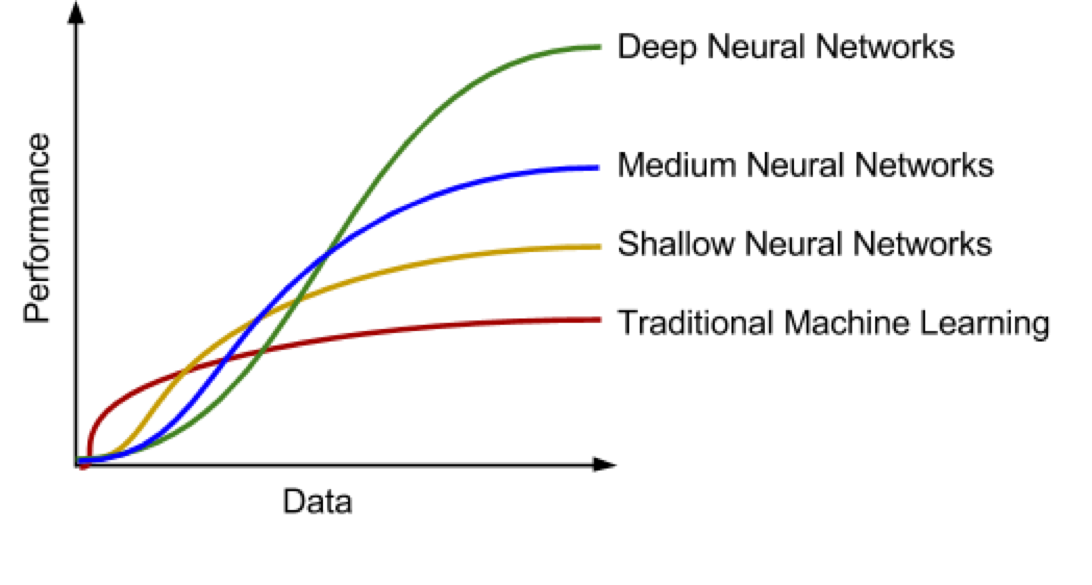
\includegraphics[scale=0.5]{images/traditionalVsDeepLearning}
\captionsetup{justification=centering}
\caption{Performance Comparision of Deep learning-based algorithms Vs Traditional Algorithms.}
\label{fig:performanceCompare}
\end{figure}


%%Applications of deep learning based anomaly detection
\begin{figure}[h]
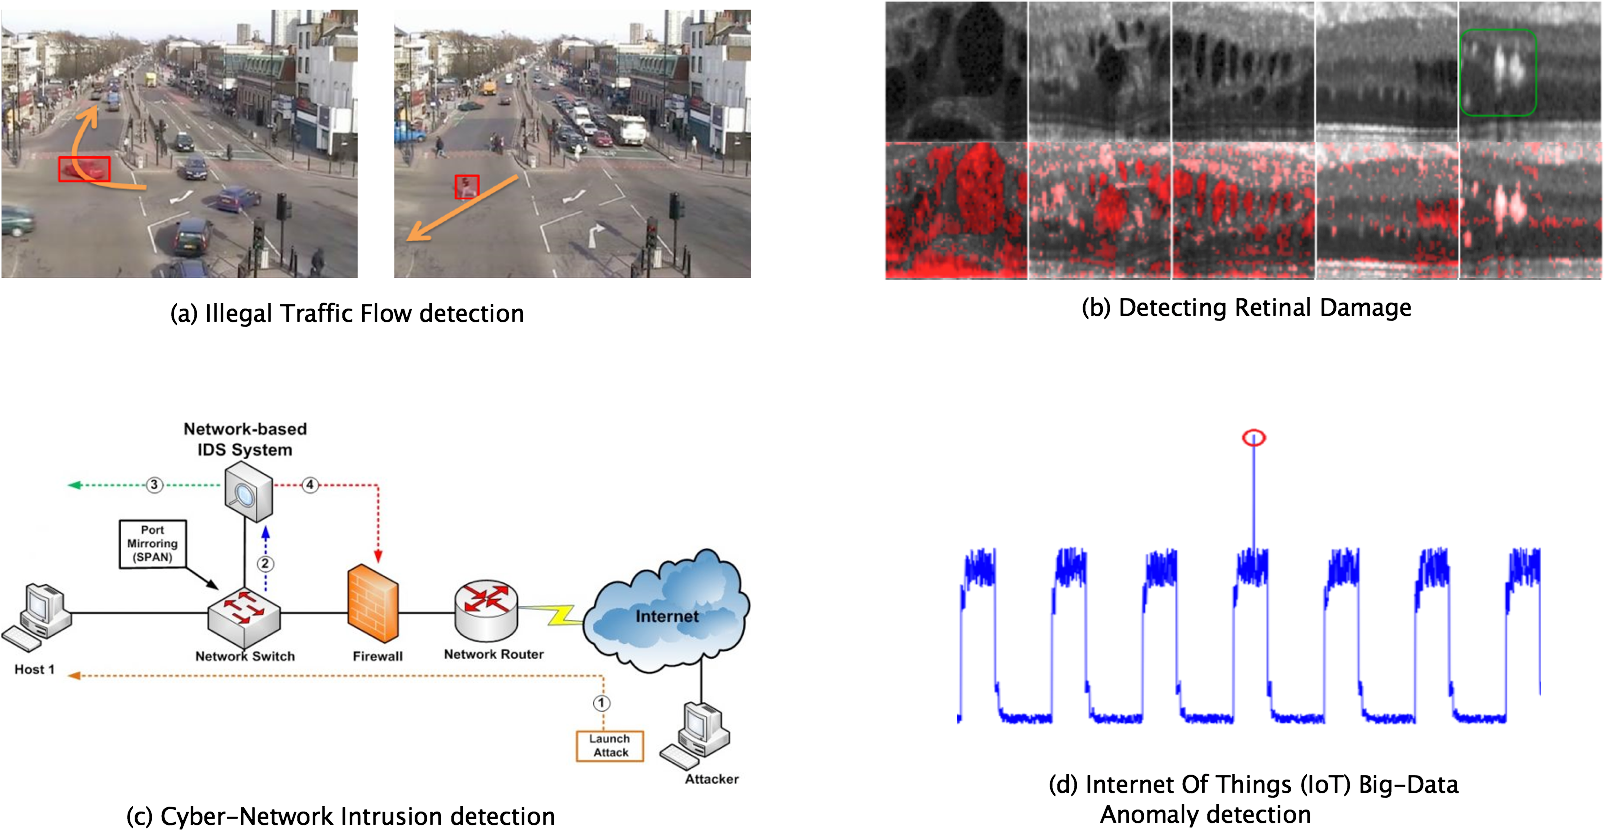
\includegraphics[scale=0.5]{images/applications}
\captionsetup{justification=centering}
\caption{Deep learning-based anomaly detection algorithms successfull applications.\\
(a) Video Survelliance, Image Analysis: Illegal Traffic detection~\cite{xie2017real}  ,  (b) Healthcare: Detecting Retinal Damage~\cite{schlegl2017unsupervised}\\
(c) Networks: Cyber-intrusion detection~\cite{javaid2016deep}  (d) Sensor Networks: Internet of Things (IoT) big-data anomaly detection~\cite{mohammadi2017deep} }
\label{fig:applications}
\end{figure}

The aim of this survey is two fold, firstly we present a structured and comprehensive overview of research methods in deep learning-based anomaly detection. Furthermore, we review the adoption of these deep-learning based methods for anomaly across various application domains and asess their effectiveness.

%anomalies
\section{ What are anomalies ?}
Anomalies  are also referred to as abnormalities, discordants, deviants, or outliers in the data mining and statistics literature~\cite{aggarwal2013introduction}.
% Anomaly Detection Definition
% \begin{figure}[h]
% 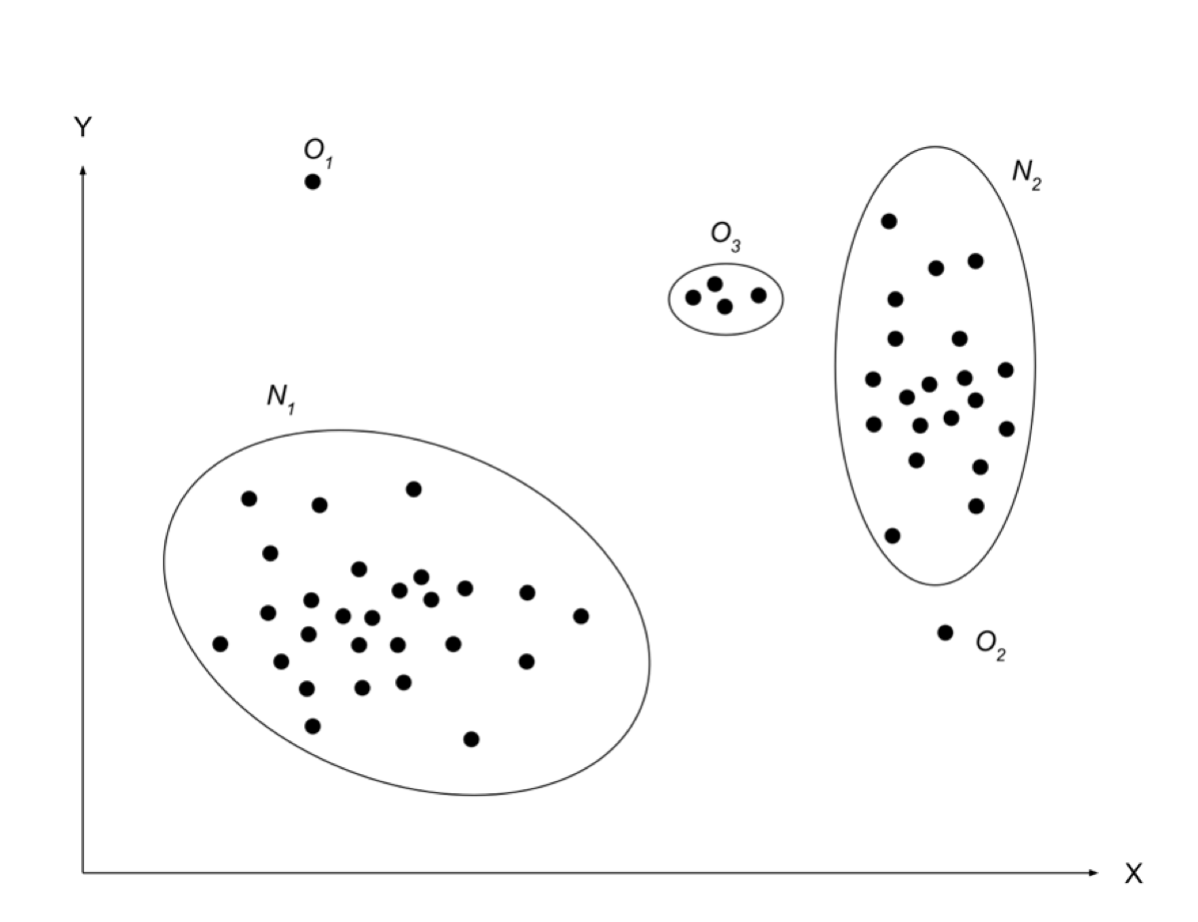
\includegraphics[scale=0.3]{images/anomalies.png}
% \caption{An illustration of anomalies in two-dimensional data set.}
% \label{fig:anomalies}
% \end{figure}

As illustrated in Figure ~\ref{fig:anomalies}, $N_{1}$ and $N_{2}$ are regions consisting of majority of observations and hence considered as normal data instance regions, whereas the region $O_{3}$, and data points  $O_{1}$ and $O_{2}$  are few data points which are located further away from the bulk of data points and hence are considered anomalies. Anomalies may arise due to several reasons, such as malicious actions, system failures, intentional fraud, etc. These anomalies reveal interesting insights about the data and are often convey valuable information about data. Therefore, anomaly detection considered an essential step in various decision-making systems.
% Novelty Detection Definition
% \begin{figure}[h]
% 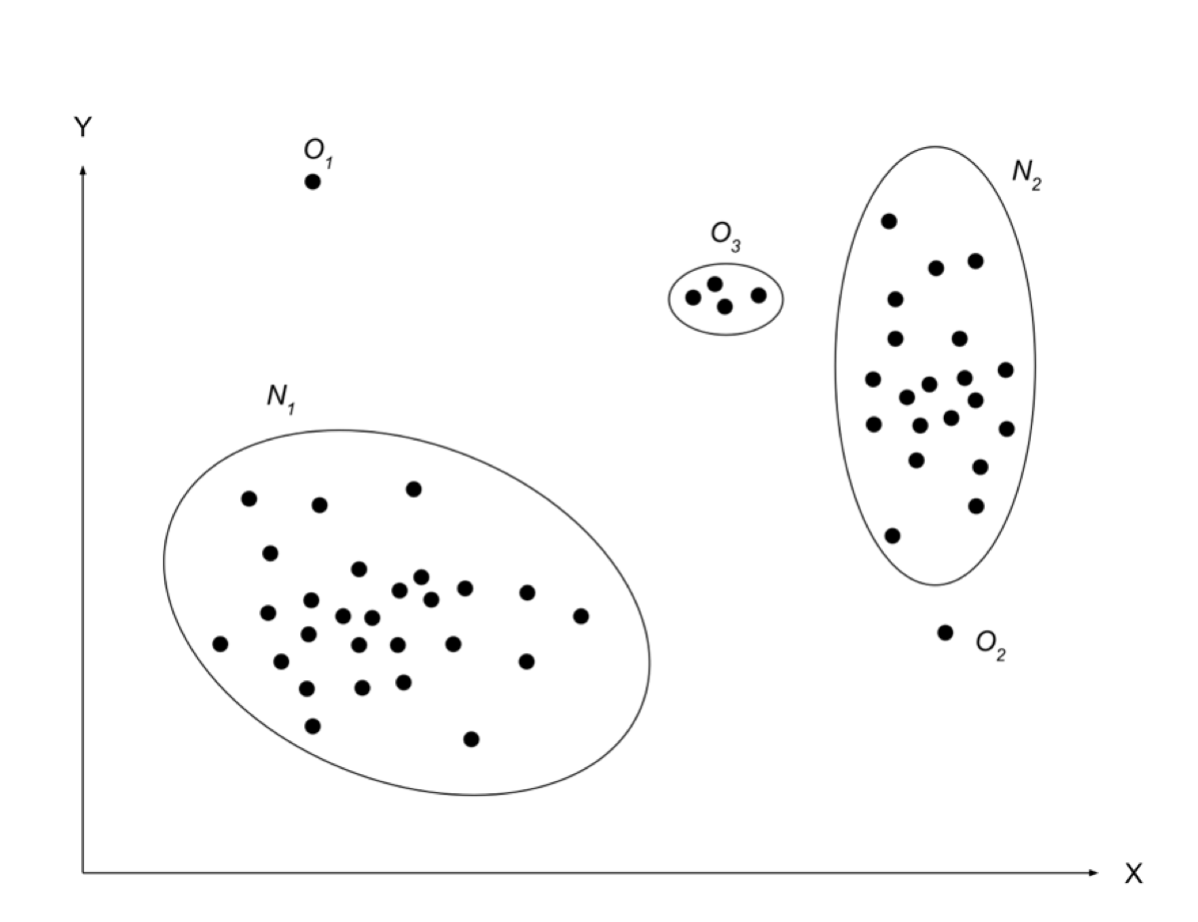
\includegraphics[scale=0.3]{images/anomalies.png}
% \caption{An illustration of anomalies in two-dimensional data set.}
% \label{fig:novelties}
% \end{figure}

% Begin of figure
\begin{figure}
  \centering
  \begin{minipage}{.48\linewidth}
    \centering
    % \subcaptionbox{}
      {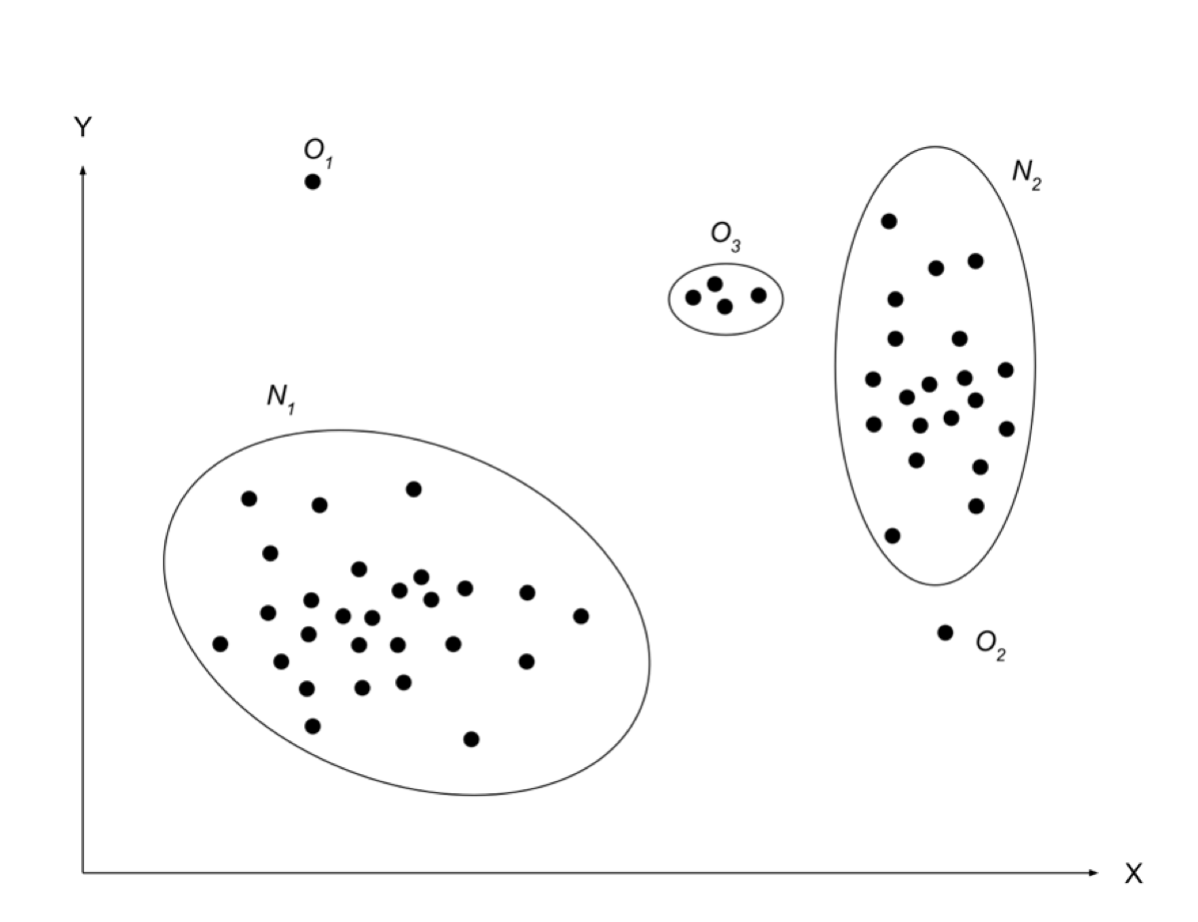
\includegraphics[scale=0.35]{images/anomalies.png}}
    \caption{Illustration of anomalies in two-dimensional data set.}
    \label{fig:anomalies}
  \end{minipage}\quad
  \begin{minipage}{.48\linewidth}
    \centering
    % \subcaptionbox{t}
      {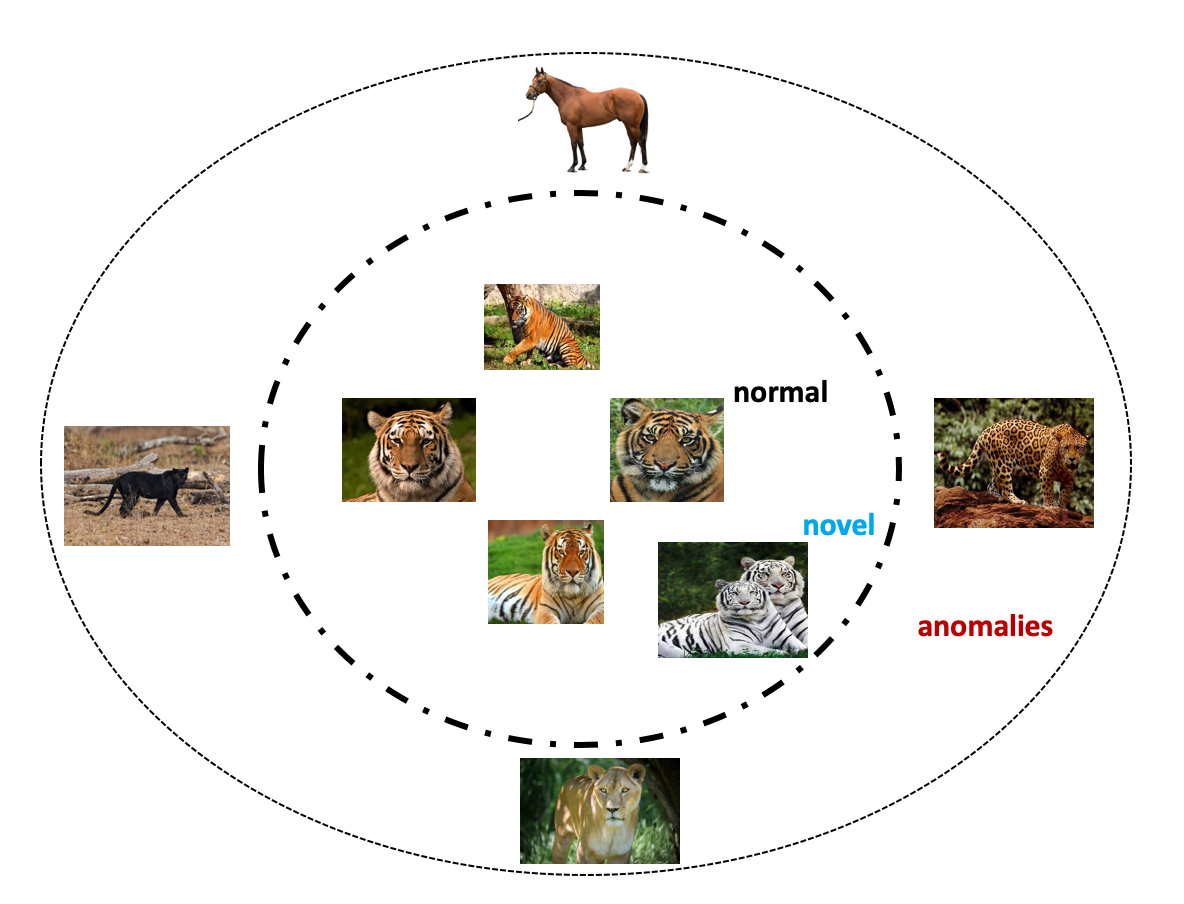
\includegraphics[scale=0.35]{images/novel.png}}
    \caption{Illustration of novelty in image data set.}
    \label{fig:novelties}
  \end{minipage}
  \bigskip

\end{figure}
% end of figure


% novelties
\section{What are novelties ?}
Novelty detection is the identification of novel (new) or unobserved patterns in the data.~\cite{miljkovic2010review}. The novelties detected are not considered as anomalous data points; instead they are incorporated into the normal data model. A novelty score may be assigned for these previously unseen data points, using a decision threshold score. ~\cite{pimentel2014review}.  The points which significanlty deviate from this decision threshold may be deemed as anomalies or outliers. For instance in Figure ~\ref{fig:novelties}  the images of \textit{(white tigers)} among normal tigers may be considered as novelty, while image of \textit{(horse, panther,lion and cheetah)} are considered as anomalies.
The techniques used for anomaly detection are often used for novelty detection and vice versa.



% Challenges : Motivation and challenges Why deep learning-based anomaly detection.
\section{Motivation and Challenges: Deep anomaly detection (DAD) techniques}
\begin{itemize}
\item Performance of traditional algorithms in detecting outliers is sub-optimal on complex image (e.g. medical images) and sequence data sets.
\item  Need for Large-scale anomaly detection : As the volume of data increases let's say to gigabytes then, it becomes nearly impossible for the traditional methods to scale to such large scale data to find outliers.
\item  Deep anomaly detection (DAD) techniques learn hierarchical discriminative features from data. This automatic feature learning capability eliminates the need of developing manual features by domain experts, therefore advocates to solve the problem end-to-end taking raw input data in domains such as text and speech recognition.
\item The boundary between normal and anomalous (erroneous) behavior is often not precisely defined  in several data domains and is constantly evolving. This lack of well defined representative normal boundary poses challenges for both conventional and deep learning-based algorithms.
\end{itemize}
% end itemize

% Begin Table
\begin{table} [ht!]
\centering
\captionsetup{justification=centering}
\caption{Comparison of our Survey to Other Related Survey Articles. \\1 \textemdash Our Survey,
2 \textemdash Kwon and Donghwoon ~\cite{kwon2017survey}, 5 \textemdash John and Derek ~\cite{ball2017comprehensive}\\
3 \textemdash Kiran  and Thomas ~\cite{kiran2018overview},            6 \textemdash Mohammadi and Al-Fuqaha ~\cite{mohammadi2017deep}\\
4 \textemdash Adewumi and Andronicus ~\cite{adewumi2017survey}       7 \textemdash Geert and  Kooi et.al ~\cite{litjens2017survey}.
}
\scalebox{0.8}{
\begin{tabular}{ |c|c|c|c|c|c|c|c|c|c| }
\hline
 & & 1&2&3&4&5&6&7 \\
\hline
\multirow{4}{6em}{Methods  }
&Supervised &\checkmark  & & & & & & \\
&Unsupervised &\checkmark & & & & & &  \\
&Hybrid Models & \checkmark& & & & & &  \\
&one-Class Neural Networks &\checkmark & & & & & &  \\
\hline
\multirow{8}{8em}{Applications  }
&Fraud Detection&\checkmark  & & &\checkmark & & & \\
&Cyber-Intrusion Detection&\checkmark  &\checkmark & & & & & \\
&Medical Anomaly Detection&\checkmark  & & & & & &\checkmark \\
&Sensor Networks Anomaly Detection&\checkmark  & & & &\checkmark & & \\
&Internet Of Things (IoT)
 Big-data Anomaly Detection&\checkmark  & & & & & \checkmark& \\
&Log-Anomaly Detection&\checkmark  & & & & & & \\
&Video Surveillance&\checkmark & &\checkmark  & & & & \\
&Industrial Damage Detection&\checkmark & & & & & & \\
\hline
\end{tabular}}
\end{table}
% End of Table


% Related Work
\section{Related Work}
Despite the substantial advances made by deep learning methods in many machine learning problems, there
is a relative scarcity of deep learning approaches for anomaly detection. Adewumi et.al~\cite{adewumi2017survey} provide a comprehensive survey of deep learning-based methods for fraud detection. A broad review of deep anomaly detection (DAD) techniques for cyber-intrusion detection is presented by Kwon et.al~\cite{kwon2017survey}. An extensive review of using DAD techniques in medical domain has been presented by Litjens et.al ~\cite{litjens2017survey}. An  overview of DAD techniques for Internet of Things (IoT) and  big-data anomaly detection is introduced by  Mohammadi et.al~\cite{mohammadi2017deep}. Sensor networks anomaly detection has been reviewed  by  Ball et.al~\cite{ball2017comprehensive}. The state-of-the-art deep learning based methods for video anomaly detection along with various categories has been presented in~\cite{kiran2018overview}. Although there are a number of reviews in applying DAD technqiues, there is shortage of comparative analysis of deep learning architecture adopted for outlier detection. For instance a substantial amount of research on anomaly detection is conducted using deep autoencoders, but there is lack of comprehensive survey of various deep architecture's best suited for a given data-set and application domain. We hope that this survey bridges this gap and provides a comprehensive reference for researchers and engineers aspiring to leverage deep learning for anomaly detection. Table I shows the set of research methods and application domains covered by our survey.

% The classification taxonomy is also present in this paper $https://www.ncbi.nlm.nih.gov/pmc/articles/PMC4836738/$
% This paper~\cite{erfani2016high} presents a hybrid approach of combining deep learning models in combination with other traditional techniques to identify outliers and obtained promising results.

% Anomaly Detection Taxonomy
\begin{figure}[h]
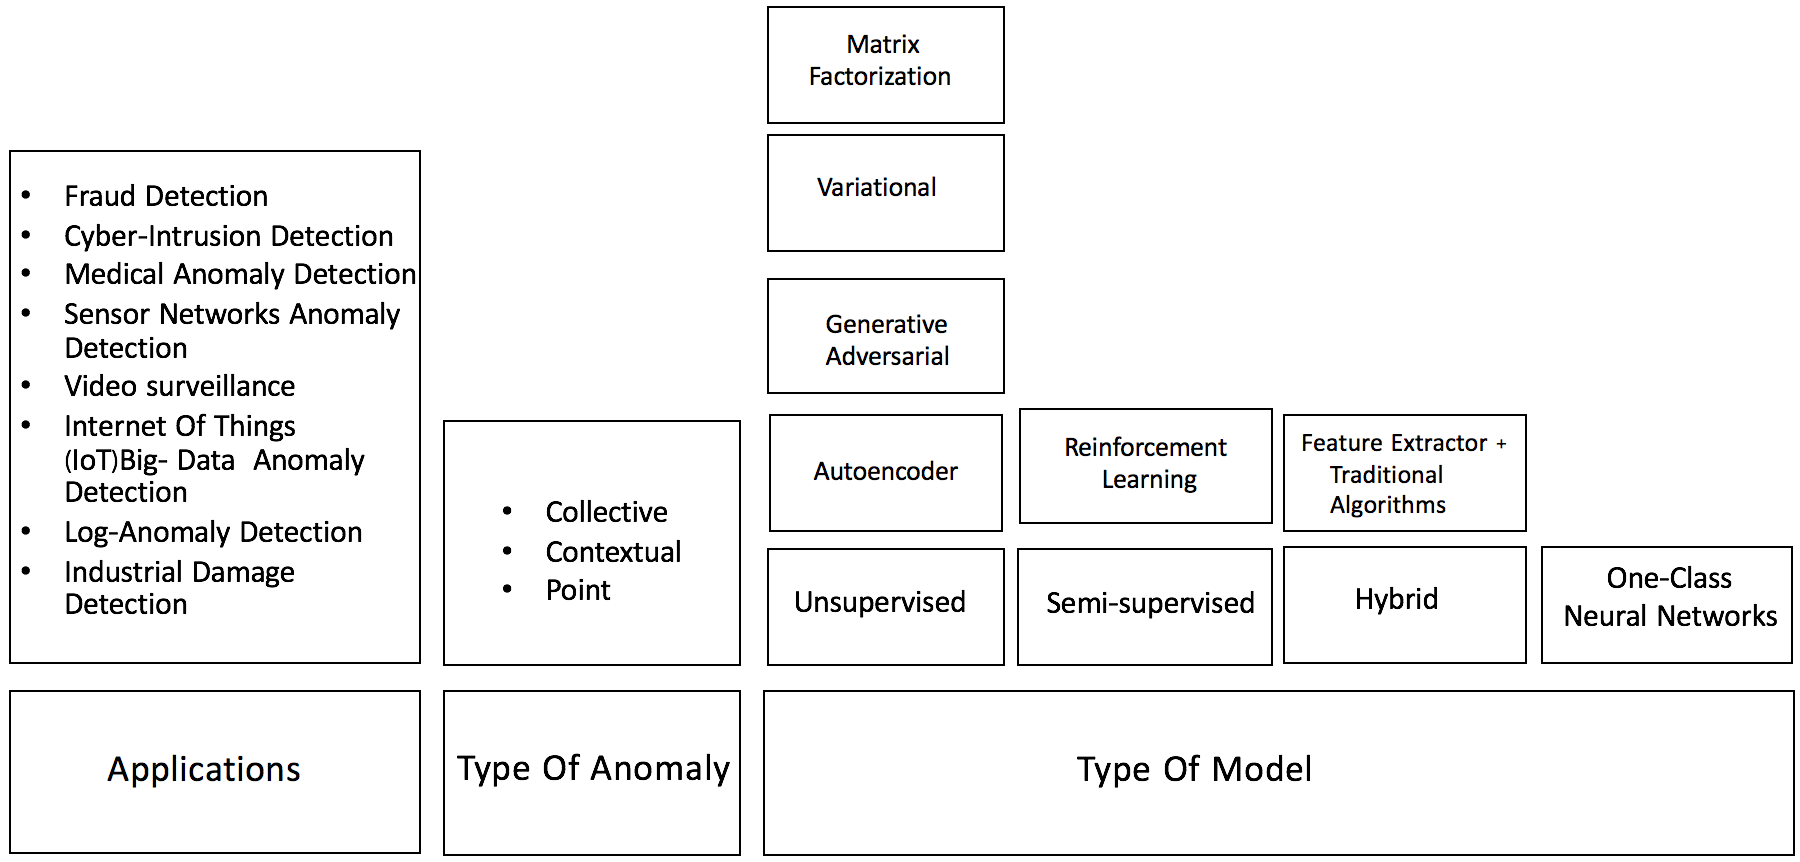
\includegraphics[scale=0.5]{images/AnomalyDetectionTaxonomy}
\caption{Key components associated with deep learning-based anomaly detection technique.}
\label{fig:surveyTaxonomy}
\end{figure}
% end of related work

%% Our Contributions
\section{ Our Contributions}
We follow survey approach of V.Chandola and A.Banerjee et.al~\cite{chandola2007outlier} for deep  anomaly detection (DAD). Our survey presents a detailed and structured overview of research and applications of DAD techniques. We summarize our main contributions as follows:
\begin{itemize}
\item Most of the existing surveys on DAD techniques either focus on a particular
application domain or specific research area of interest~\cite{kiran2018overview,mohammadi2017deep,litjens2017survey,kwon2017survey,adewumi2017survey,ball2017comprehensive}.
This review aims to provide a comprehensive outline of state-of-the art research in DAD techniques as well as several real world applications these techniques are discussed.
\item In recent years a number of new deep learning based anomaly detection techniques  with greatly reduced computational requirements have been developed. The purpose of this paper is to survey these techniques and classify them into organised schema for better understanding. We introduce two more sub-categories Hybrid models ~\cite{erfani2016high} and one-class neural networks techniques~\cite{chalapathy2018anomaly} as illustrated in Figure~\ref{fig:surveyTaxonomy} based on the choice of training objective. For each categories we discuss both the assumptions and techniques adopted for best performance. Furthermore within each category, we also present the challenges, advantages and disadvantages and provide an overview of computational complexity of DAD methods.
\end{itemize}

% Organization of the paper
\section{Organization}
This survey is organized by following structure described in Figure~\ref{fig:surveyTaxonomy}.
In Section~\ref{sec:aspectsOfAnomalyDetection}, we identify the various aspects that determine the formulation of the problem and highlight the richness and complexity associated with anomaly detection.
We introduce and define two types of models: contextual and collective or group anomalies. In Section~\ref{sec:applicationsOfDLAD}, we briefly describe the different application domains to which deep learning-based anomaly detection has been applied. In subsequent sections we provide a categorization of deep learning-based techniques based on the research area to which they belong.  Based on training objectives employed and availability of labels  deep learning-based anomaly detection techniques  can be categorized into supervised (Section~\ref{sec:supervisedDAD}), unsupervised (Section ~\ref{sec:unsupervisedDAD}), hybrid (Section~\ref{sec:hybridModels}), and one-class neural network  (Section~\ref{sec:oneclassNN}). For each category of techniques we also discuss their computational complexity for training and testing phases. In Section~\ref{sec:typeBasedAD} we discuss  point, contextual, and collective (group) deep learning-based anomaly detection techniques. We present some discussion of the limitations and relative performance of various existing techniques in Section~\ref{sec:relativeSOW}. Section~\ref{sec:conclusion} contains
concluding remarks.




% Group deviation detection involves the discovery of group behaviours which significantly deviate from  expected   patterns. With  increased availability of multifaceted information, there is a growing trend towards research involving groups or collections of observations.   Group anomaly detection (GAD) is the process of identifying groups that are not consistent with regular group behaviours while group change detection (GCD) estimates significant deviations in the state of a group over  time. Since both GAD and GCD problems share fundamental ideas, this  Even though GAD usually involves time-independent applications and GCD relates to time-dependent groups, both problems share a common framework  and  fundamental ideas.
% thesis elaborates on group deviation detection techniques in static and dynamic situations.


% % \subsection{Definition of Groups} %
% A group is simply defined as a collection of two or more related data instances.    %F\~{a}rber et al. \cite{ClusterEval} even discusses how known group labels may not correspond to inherently clustered points.
% In GAD, a group anomaly has  significantly different  statistical properties  with respect to other groups whereas GCD involves detecting  a significant change in a group  with respect to past behaviour.   Group structures may be known a priori such as words in a document otherwise when group   memberships between instances are unknown, additional information or clustering algorithms are required.
% %  Thus the initial definition of groups greatly  affects subsequent analysis and results of detecting group deviations.




% More specifically,  Xiong et al.  \cite{MGM} categorise group deviations as either point-based or distribution-based for GAD applications.   Point-based anomalous groups are where all of the members are also pointwise anomalies. Similarly in GCD, a point-based group change signifies that a large proportion of  time series in a group exhibit significant deviations.   On the other hand, a  distribution-based group anomaly is where  individual  instances conform to regular patterns however the collection of points is anomalous. Likewise, a distribution-based change in a group over time occurs when individual time series exhibit regular behaviour however the  collective process is significantly different to historical patterns.



% \begin{figure}[h]
% \centering
% % \begin{subfigure}[b]{0.6\textwidth}
% %                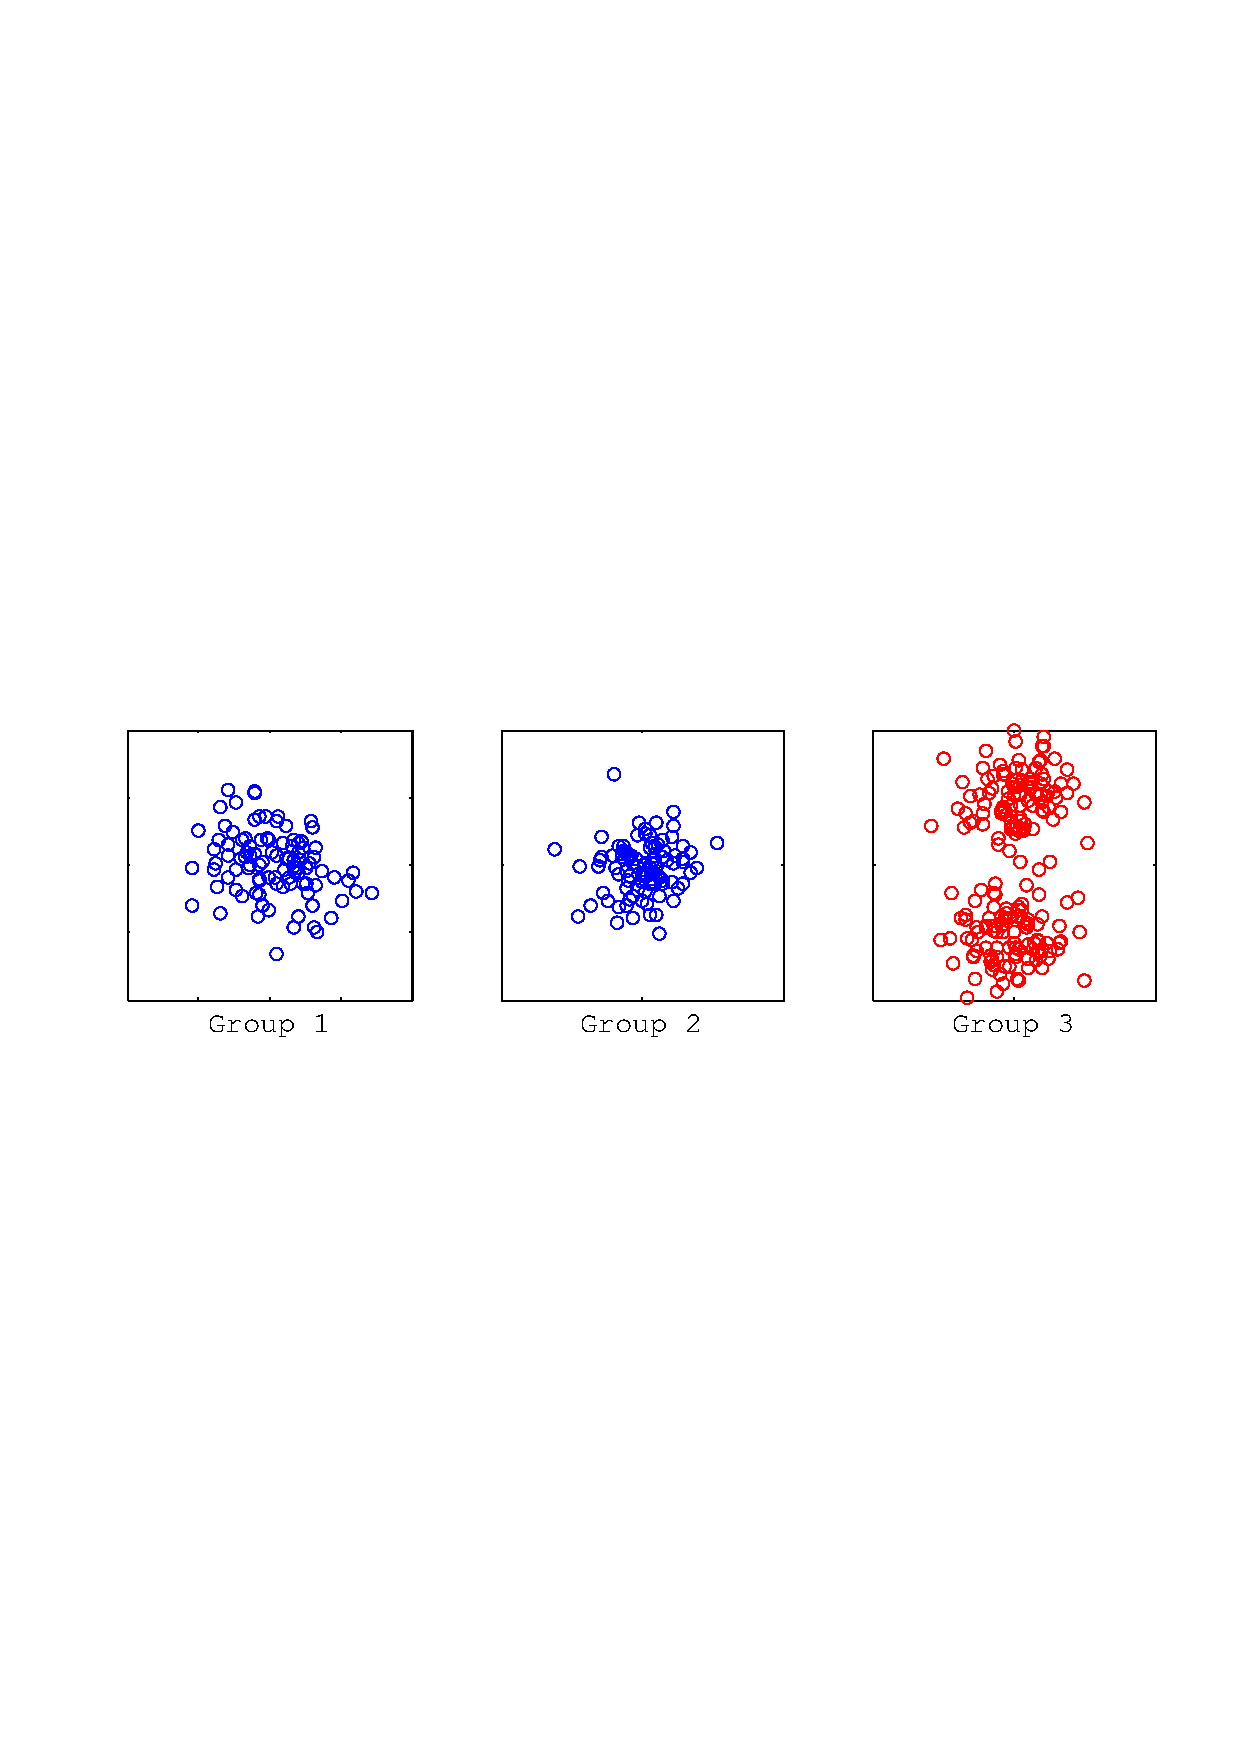
\includegraphics[width=\linewidth,trim=3cm 12cm 3cm 12cm]{FIGURES/Ex1}
% %                \caption{A significant deviation in scale or shape.}
% %        \end{subfigure}%
%  \begin{subfigure}[b]{1\textwidth}
%                 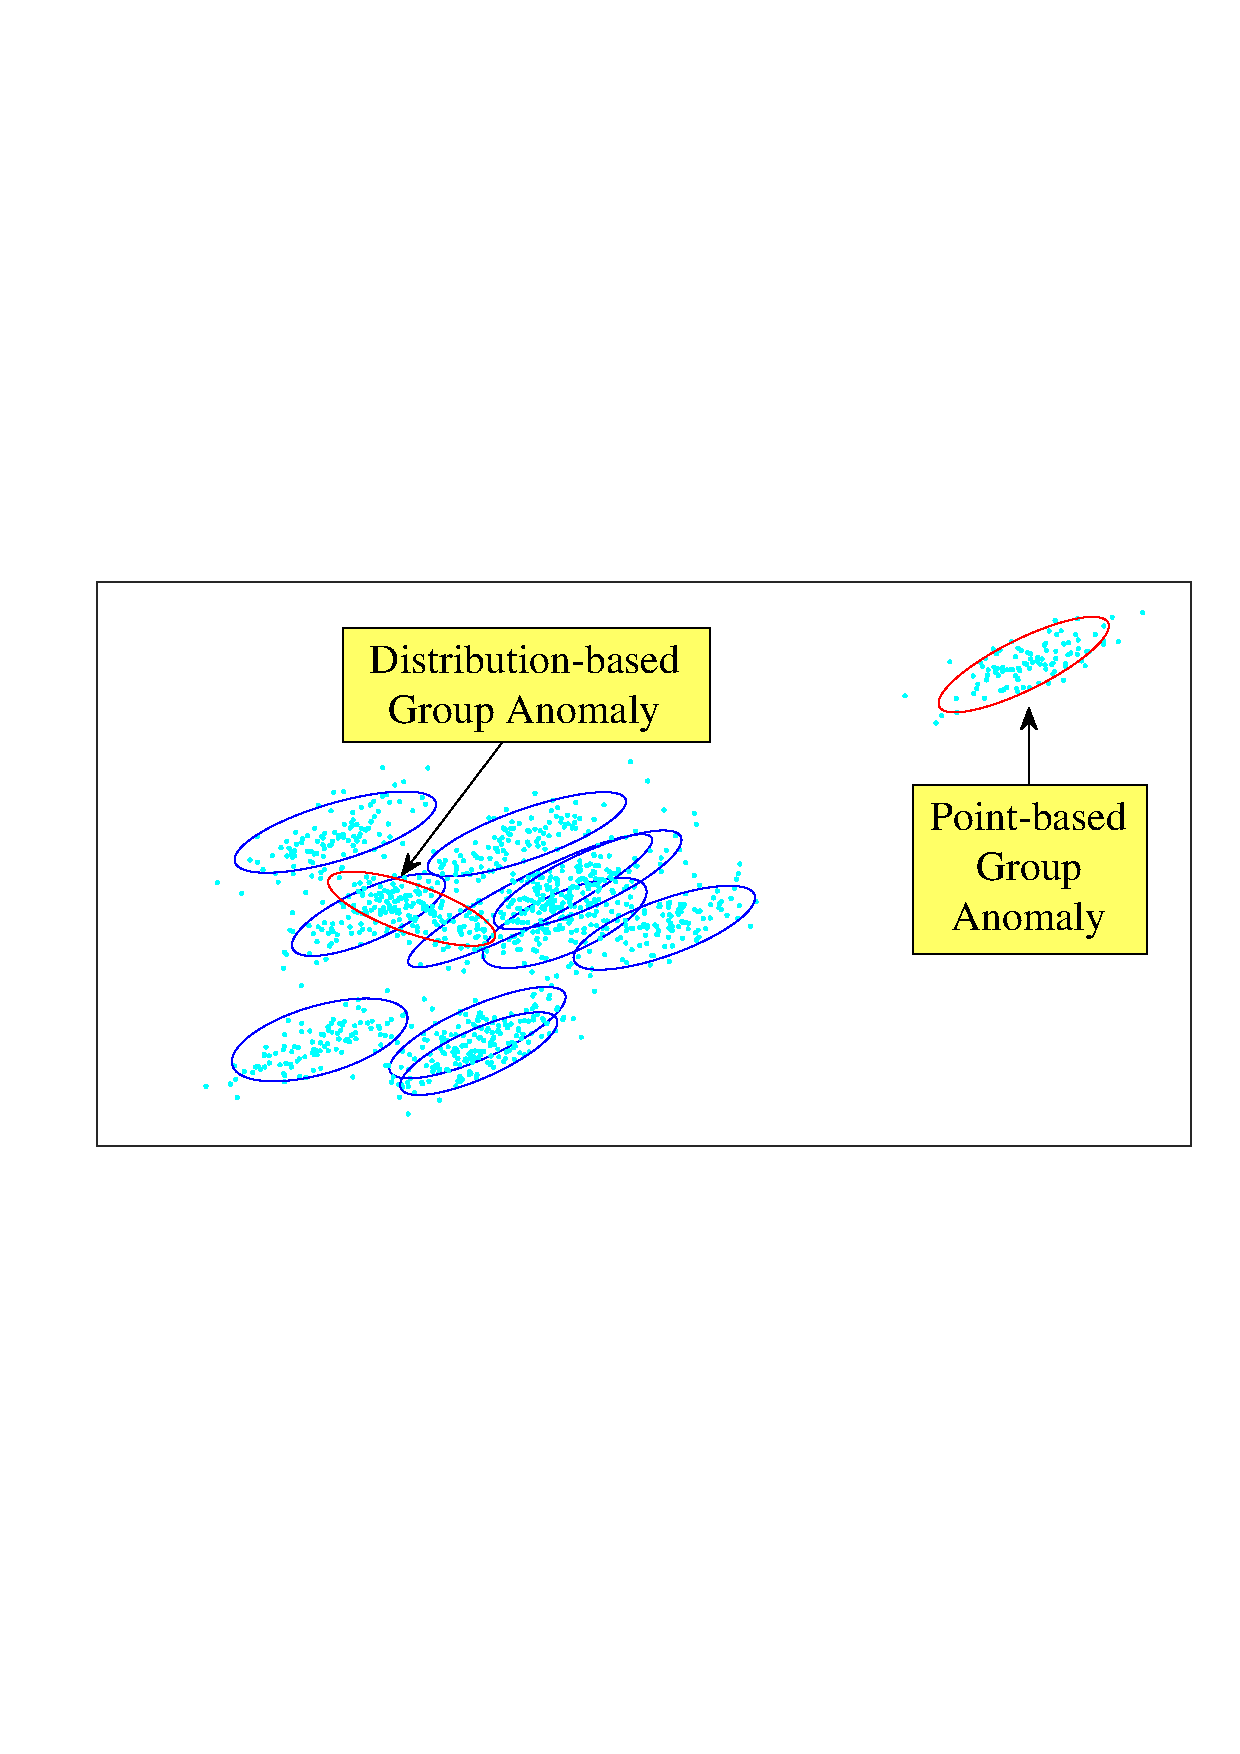
\includegraphics[width=9cm,
%                 height=5cm,trim=0cm 10cm 6cm 10cm]{FIGURES/gad_ex}
%                 \caption{Two types of group anomalies; point-based group anomaly is a collection of anomalous points  %that are anomalous with respect to a central location
%                  whereas in this example, a  distribution-based group anomaly contains non-anomalous observations however as a  collection,  significantly differs with a rotated  correlation structure.                    }
%         \end{subfigure}%
% \hfill
% \vspace{2mm}
% \vfill
%  \begin{subfigure}[b]{1\textwidth}
%  \centering
%                 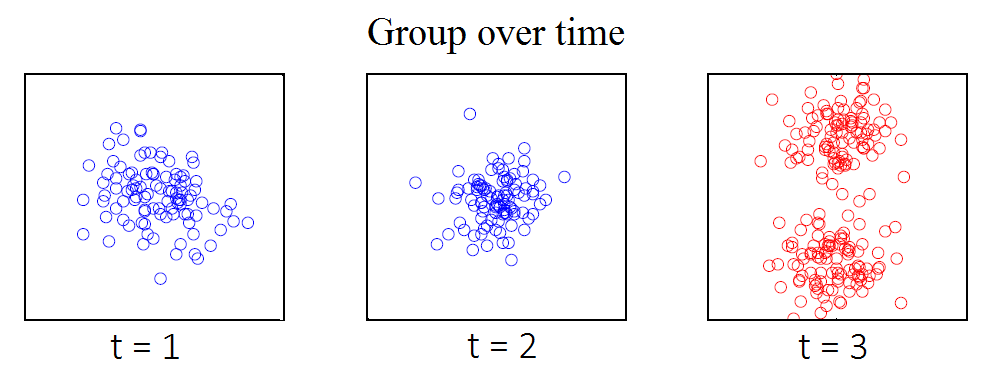
\includegraphics[width=10cm, height=4cm,trim=0cm 0cm 0cm 0cm]{FIGURES/gcd_ex}
%                 \caption{ Distribution-based group change at $t=3$ has significantly different  scale and shape.
% }
%   \end{subfigure}%
% \caption{Examples of group behaviours that clearly deviate in terms of different statistical properties.
% }
% \label{Fig:Intro1}
% \end{figure}

%  Figure \ref{Fig:Intro1}  highlights examples of group deviations that occur in  GAD and  GCD applications. For GAD, a point-based group anomaly  differs by central location whereas the distribution-based group anomaly has a rotated correlation structure. The GCD example illustrates   a group change as a significant deviation in scale and shape over time.  In real-world applications, Xiong et al. \cite{MGM} detect  rotated galaxy clusters whereas Chen et al. \cite{GLETS}  identify deviating scale and shape of a  stock portfolio over time.


% GAD and GCD methods have many advantages over  pointwise methods for detecting group deviations.
% %Pointwise anomaly and change detection focus on the study of individual data instances that do not conform with the expected pattern.
%  Many pointwise anomaly detection methods are also not compatible  in detecting  group deviations so  more specialised techniques are required.
%  For example,  Muandet et al.	\cite{OCSMM} detect Higgs bosons as a group of collision events  in high energy particle physics while a group of multiple sensor networks in Chen and Yu \cite{chen2016collaborative}, allow for a robust  detection of  distributed denial-of-service attacks. Group deviation detection  techniques also result in fewer false positives than pointwise approaches as a greater number of observations occur in real-world group applications. %provide a better characterization of group behaviours.



% Detecting group anomalies has a variety of interesting real-world results. % physical real-world  applications.  %that motivate different avenues of research.
%   Muandet et al.	\cite{OCSMM} investigate GAD in high energy particle physics where Higgs bosons are observed as slight excesses in a collection of collision events rather than individual  instances. In Guevara et al. \cite{SMDD}, an anomalous galaxy cluster is identified by an irregular proportion of color pixels while Xiong et al. \cite{FGM}  analyse unusual vorticity in fluid turbulence data.
% %where a group anomaly represents  in  fluid dynamics.
% Textual data is also studied for GAD where a document is considered a group of words.
% Using word inputs from scientific publications, Yu et al. \cite{GLAD}  %investigate  in order to understand the structure of certain research communities. I
% detect  possible irregular communities of co-authors that reveal unusual research trends.  By analysing documents from news articles, Soleimani and Miller \cite{ATD} discover novel topics in a document corpus.   Using text data from Amazon reviews, Mukherjee et al.  \cite{GroupReviewSpam} examine groups of spammers that collaborate in writing fake reviews.

%  %infer regular topics   such as $`\mathtt{rec.sport.baseball}'$  and $`\mathtt{ talk.politics.misc}'$. An anomalous cluster in this case consists of novel topics that are unobserved in the training corpus such as $`\mathtt{rec.sport.hockey}'$ and \\$`\mathtt{talk.politics.mideast}'$.

% %There are many other applications where GAD and GCD techniques offer interesting results.

%   A group over time for GCD is also studied across a variety of domains.  Wong et al. \cite{wong-rule} %investigate different demographic groups admitted to  emergency departments in hospitals in a major US city.   A
%    detect significant changes in demographic groups that are admitted to  emergency departments where changes represent  potential disease outbreaks.
%   Chen et al. \cite{GLETS} monitor how a group of  stocks
%   may disband with dissimilar behaviors over time while seemingly uncorrelated time series may form a more cohesive collection.   Using multiple sensor data, Xie and Siegmund  \cite{xie2013} explore sequential change detection in a proportion of time series in a group over time.
%   Another example of real-world GCD event occurred when  five of the largest private health insurers in Chile colluded to unfairly reduced  coverage of healthcare plans over time \cite{Chile}.   Thus there are many interesting and meaningful insights that are gained from GAD and GCD applications.
% The  main contributions  of our thesis are  summarised as follows: %\vspace{-1mm}
% \begin{enumerate}
% %\item {\bf Clearer Understanding:}
% %This survey provides an underlying structure for   both group anomaly detection (GAD) and group change detection (GCD) problems.      % Figure \ref{Fig:Framework}  builds upon the anomaly detection from Chandola \cite{Chandola}
% \item {\bf Detailed Overview:}
%  We clearly formulate the problem of group anomaly detection (GAD) and group change detection (GCD) with detailed descriptions of state-of-the-art techniques. %Although deep generative models have been applied in various image applications, they have not been applied to the GAD problem. % of detecting group anomalies.
% \item {\bf Static GAD}: Deep generative models (DGMs) are proposed for solving the GAD problem for complex group distributions with a high detection performance under certain conditions.
% \item {\bf Dynamic GCD:} We propose the GT$\Delta$ algorithm  for sequentially detecting temporal changes in  a group of stochastic processes with advantages such as a robustness to outliers,  better interpretation and effective detection results.
% \end{enumerate}

\section{Different aspects of deep learning-based anomaly detection. }
\label{sec:aspectsOfAnomalyDetection}
This section identifies and discusses the different aspects of deep learning-based anomaly detection.

%%%%%%%%%%%%%%%%%%%%%%%% Begin of  Nature of Input data %%%%%%%%%%%%%%%%%%%%%%%%
\subsection{ Nature of Input Data}
The choice of deep neural network architecture in deep anomaly detection methods primarily depends on the nature of input data. Input data can be broadly classified into sequential (eg, voice, text, music, time series, protein sequences) or non-sequential data (eg, images, other data). Table~\ref{tab:dataTypeModelArchitecture} illustrates the nature of input data and deep model architectures used in anomaly detection. Additionally input data depending on the number of features (or attributes) can be further classified into either low or high-dimensional data. DAD techniques have been to learn complex hierarchical feature relations within high-dimensional raw input data ~\cite{lecun2015deep}. The number of layers used in DAD techniques is driven by the dimensionality of input data, deeper networks are shown to produce better performance on high dimensional data. Later on in the Section ~\ref{sec:deepDADModels}  various models considered for outlier detection are reviewed at depth.

%% Create a table with Type of data and kind of architecture suitable for anomaly detection.
\begin{table}
\centering
\begin{tabular}{ |c|c|c|c| }
\hline
Type of Data & Examples & DAD model architecture  \\ [0.5ex]
\hline
\multirow{3}{3em}{Sequential} & Video,Speech &  \\
&Protein Sequence,Time Series  & CNN, RNN, LSTM  \\
&Text (Natural language)  &  \\
\hline
\multirow{2}{3em}{Non-Sequential} & Image,Sensor &  \\
&Other (data)  & CNN, AE and its variants  \\
\hline
\end{tabular}
\caption{Table illustrating nature of input data and corresponding deep anomaly detection model architectures proposed in literature.
        \\CNN: Convolution Neural Networks, LSTM : Long Short Term Memory Networks \\
         AE: Autoencoders. }
\label{tab:dataTypeModelArchitecture}
\end{table}
% End of table
%%%%%%%%%%%%%%%%%%%%%%%% End of  Nature of Input data %%%%%%%%%%%%%%%%%%%%%%%%


%%%%%%%%%%%%%%%%%%%%%%%% Begin  Type of models %%%%%%%%%%%%%%%%%%%%%%%%
\subsection{Based on Availability of labels}
Labels indicate whether a chosen data instance is normal or outlier. Anomalies are rare entities hence it is very  difficult to obtain their labels. Furthermore anomalous behaviour may change over time, for instance  the nature of anomaly had changed so significantly and that it  remained unnoticed at Maroochy water treatment plant, for a long time which resulted in leakage of 150 million litres of untreated sewerage to local waterways ~\cite{ramotsoela2018survey}.\\
Deep anomaly detection (DAD) models can be categorized into three categories based on extent of availability of labels. (1) Supervised anomaly detection (SAD). (2) Semi-Supervised anomaly detection (SSAD). (3) Unsupervised anomaly detection (USAD).

\subsubsection{Supervised anomaly detection:}
\label{supervised_learning}
Supervised anomaly detection involves training a supervised binary or multi class classifier, using labels of both normal and anomalous data instances. Supervised DAD models, formulated as multiclass classifier in chapter IV of thesis, aids in identifying a legitimate drug name mention ~\cite{chalapathy2016investigation}.A supervised classifier trained on sequential text data used to identify a valid clinical concept~\cite{chalapathy2016bidirectional} is shown to produce state-of-the-art results.
Despite supervised methods are shown to perform well, supervised DAD methods are not as popular as semi-supervised or unsupervised methods owing to lack of availability of labeled training samples. Moreover the performance of supervised classifier used as anomaly detector is suboptimal due to class imbalance (the total number of positive class instances are far more than the total number of (negative) class of data). Therefore we do not consider the review of supervised DAD methods in this survey.


\subsubsection{Semi-supervised anomaly detection:}
\label{semi_supervised_learning}
The labels of normal instances are far more easy to obtain than anomalies, as a result semi-supervised DAD techniques are more widely adopted, these techniques leverage existing labels of single (normally positive class) to separate outliers. One common way of using deep autoencoders  in anomaly detection is to train them in a semi-supervised way on data samples with no anomalies. With sufficient training samples, of normal class autoencoders would produce low reconstruction errors for normal instances, over anomalous events.
~\cite{wulsin2010semi,nadeem2016semi,song2017hybrid}. We consider detailed review of these methods in  Section~\ref{sec:semi_supervised_DAD}.

%% Taxonomy of Models
%performance comparision
\begin{figure}[h]
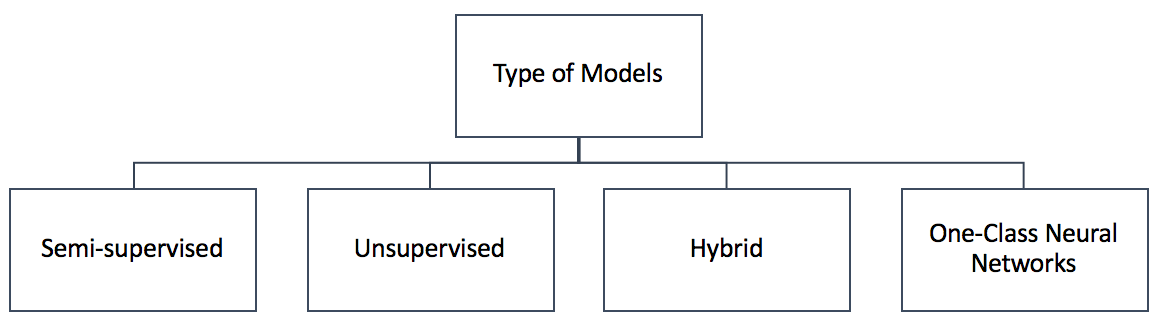
\includegraphics[scale=0.5]{images/TypeOfModels}
\captionsetup{justification=centering}
\caption{Taxonomy based on type of deep learning models for anomaly detection.}
\label{fig:typeOfModels}
\end{figure}

\subsubsection{Unsupervised anomaly detection (USAD):}
\label{sec:USAD}

Unsupervised anomaly detection techniques detect outliers solely based on intrinsic properties of the data instances. USAD techniques are used in automatic labelling of unlabelled data samplessince labeled data is very hard to obtain ~\cite{patterson2017deep}. Variants of USAD models~\cite{tuor2017deep} are shown to outperform traditional methods such as principal component analysis (PCA) ~\cite{wold1987principal}, support vector machine (SVM) ~\cite{cortes1995support} and Isolation Forest~\cite{liu2008isolation} techniques in applications domains such as health and cyber security.
Autoencoders are the core of all USAD models. These models assume the high prevalence of normal instances than abnormal data instances failing which would result in high false positive rate. Additionally unsupervised learning algorithms such as restricted Boltzmann machine (RBM)~\cite{sutskever2009recurrent}, deep Boltzmann machine (DBM), deep belief network (DBN)~\cite{salakhutdinov2010efficient}, generalized denoising autoencoders~\cite{vincent2008extracting} , recurrent neural network (RNN)~\cite{rodriguez1999recurrent} Long short term memory networks~\cite{lample2016neural} which are used to detect outliers are discussed in detail in Section ~\ref{sec:rnn_lstm_gru}.

\subsection{Based on training objective}
In this survey we introduce two new categories of deep anomaly detection (DAD) techniques based on training objective employed 1) Deep hybrid models (DHM). 2) One class neural networks (OC-NN).

\subsubsection{Deep Hybrid Models (DHM):}
\label{sec:DHM}

Deep hybrid models for anomaly detection use deep neural networks mainly autoencoders as feature extractors, the features learnt within the hidden representations of autoencoders are input to traditional anomaly detection algorithms such as one-class SVM (OC-SVM) to detect outliers~\cite{andrews2016detecting}. Figure~\ref{fig:HybridDeepModels} illustrates  the deep hybrid model architecture used for anomaly detection. Following the success of transfer learning to obtain rich representative features  from models pre-trained on large datasets,  hybrid models have also employed these pre-trained transfer learning models as feature extractors with great success ~\cite{pan2010survey}. A variant of hybrid model was proposed by  Ergen et.al~\cite{ergen2017unsupervised} which considers joint training of feature extractor alongwith OC-SVM (or SVDD) objective to maximize the detection performance. A notable shortcoming of these hybrid approaches
is the lack of trainable objective customised for anomaly detection, hence these models fail to extract rich differential features to detect outliers.  In order to overcome this limitation customised objective for anomaly detection such Deep one-class classification~\cite{ruff2018deep}and  One class neural networks~\cite{chalapathy2018anomaly} are introduced.

\begin{figure*}
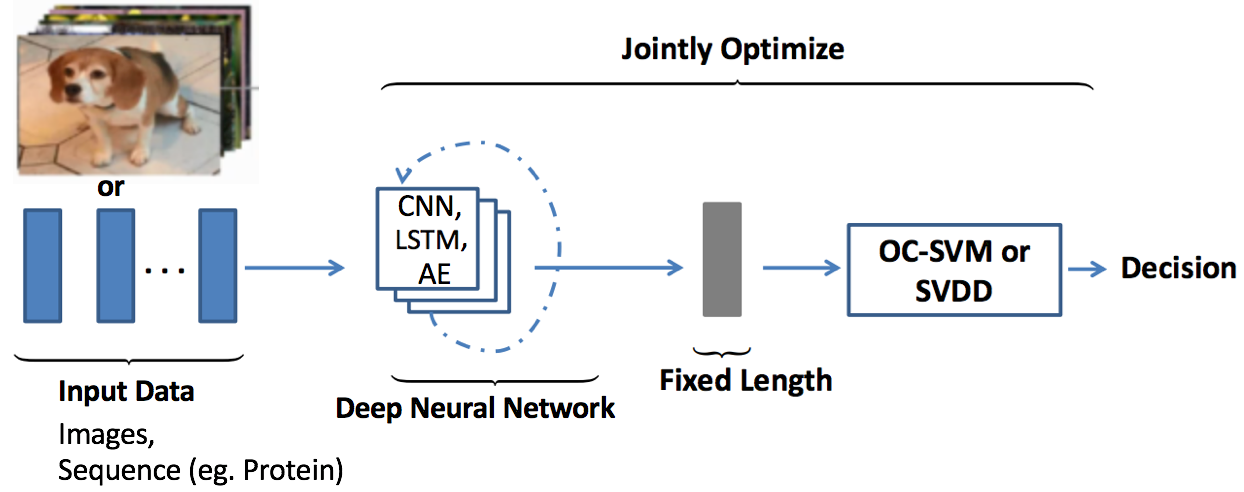
\includegraphics[scale=0.5]{images/HybridDeepModels}
\captionsetup{justification=centering}
\caption{Deep Hybrid Model Architecture.}
\label{fig:HybridDeepModels}
\end{figure*}

\subsubsection{One-Class Neural Networks (OC-NN):}
\label{sec:oc-nn}

One class neural network~\cite{chalapathy2018anomaly} methods are inspired by kernel-based one-class classification which combines the ability of deep networks to extract progressively rich representation of data with the one-class objective of creating a tight envelope around normal data. The OC-NN approach breaks new ground for the following crucial reason: data representation in the hidden layer is driven by the OC-NN objective and is thus customized for anomaly detection. This is a departure from other approaches which use a hybrid approach of learning deep features using an autoencoder and then feeding the features into a separate anomaly detection method like one-class SVM (OC-SVM).  The details of training and evaluation of one class neural networks is discussed in Section [XX] . Another variant of one class neural network architecture Deep Support Vector Data Description (Deep SVDD)~\cite{ruff2018deep} trains deep neural network to extract common factors of variation by closely mapping the normal data instances to the center of sphere, is shown to produce state-of-the-art results on MNIST and CIFAR-10 datasets.


%%%%%%%%%%%%%%%%%%%%%%%% End  Type of Models %%%%%%%%%%%%%%%%%%%%%%%%

\vspace{0.6cm}
\subsection{Type of Anomaly}
\label{sec:typeBasedAD}
Anomalies can be broadly  classified into three types: point anomalies, contextual anomalies and collective anomalies. Deep anomaly detection (DAD) methods have been shown to detect all three types of anomalies with great success.

% classification tree
\begin{figure}[h]
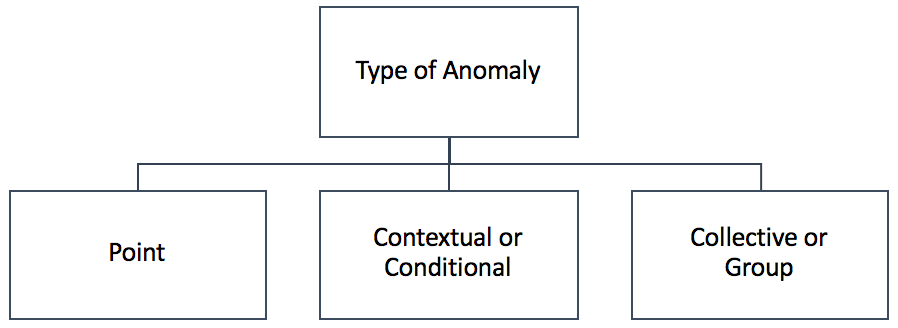
\includegraphics[scale=0.5]{images/TypeOfAnomaly}
\captionsetup{justification=centering}
\caption{Deep learning techniques classification based on type of anomaly.}
\label{fig:typeOfAnomaly}
\end{figure}


% Point Anomaly
\subsubsection{Point Anomalies.}
The majority of work in literature focuses on point anomalies. Point anomalies often represent an irregularity or deviation that happens randomly and may have no particular interpretation. For instance in Figure~\ref{fig:PointAndCollectiveAnomaly} a credit card transaction with high expenditure recorded at
\textit{Monaco} restaurant seems a point anomaly since it significantly deviates from the rest of the transactions. Several real world applications, considering point anomaly detection are reviewed in Section~\ref{sec:applicationsOfDLAD}.

% Contextual Anomaly
\subsubsection{Contextual Anomaly Detection.}
\label{sec:contextualanomalies}
Contextual anomaly also referred as conditional anomaly is a data instance that could be considered as anomalous in some specific context~\cite{song2007conditional}. The contextual anomaly is identified by considering both contextual and behavioural features.
The contextual features, normally used are time and space. While the behavioral features may be pattern of spending money, occurence of system log events, or any feature used to describe the normal behaviour.
Figure ~\ref{fig:temperatureContextual} illustrates the example of contextual anomaly considering temperature data indicated by a drastic drop just before June, this value is not indicative of a normal value found during this time. Figure ~\ref{fig:deeplogContextual} illustrates using deep Long Short-Term Memory (LSTM)~\cite{hochreiter1997long}  based model to identify anomalous system log events ~\cite{du2017deeplog} in a given context.

% Begin of figure
\begin{figure}
  \centering
  \begin{minipage}{.48\linewidth}
    \centering
    % \subcaptionbox{}
      {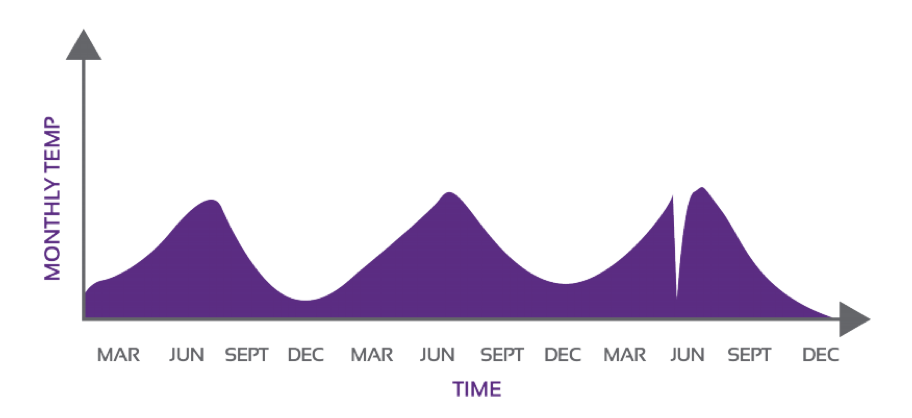
\includegraphics[scale=0.35]{images/temperature.png}}
    \caption{Illustration of contextual anomaly detection in two-dimensional temperature data set.}
    \label{fig:temperatureContextual}
  \end{minipage}\quad
  \begin{minipage}{.48\linewidth}
    \centering
    % \subcaptionbox{t}
      {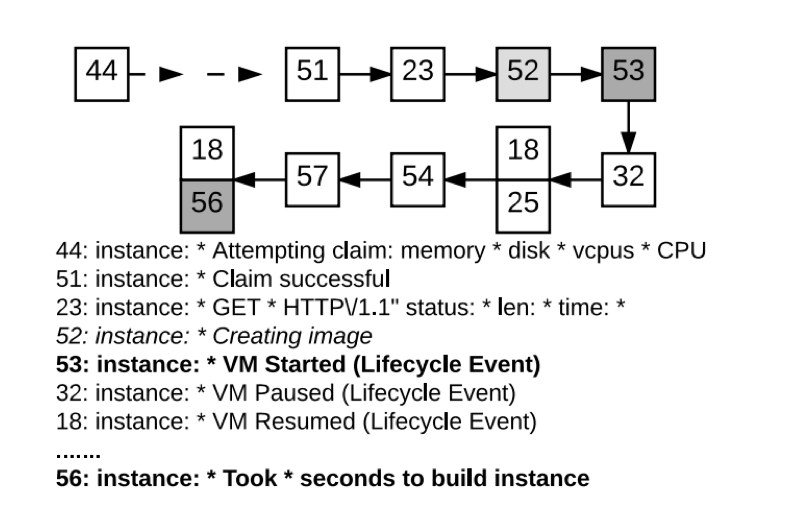
\includegraphics[scale=0.35]{images/deeplog.png}}
    \caption{Illustration of contextual anomaly detection in system logs.}
    \label{fig:deeplogContextual}
  \end{minipage}
  \bigskip

\end{figure}
% end of figure


% classification tree
% \begin{figure}[h]
% 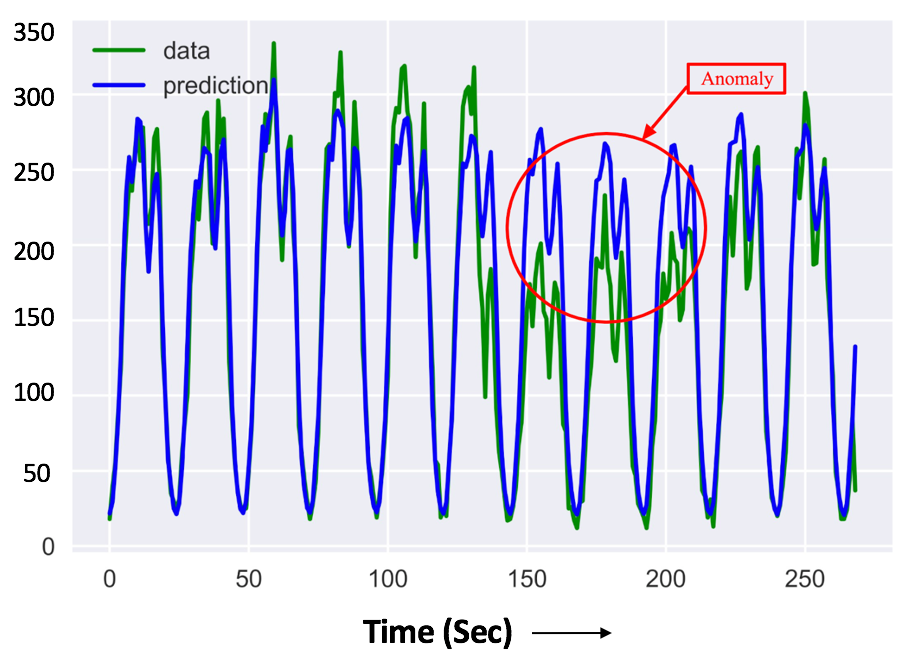
\includegraphics[scale=0.5]{images/ContextualAnomaly}
% \captionsetup{justification=centering}
% \caption{Predicted Vs Actual Data : Illustrating Contextual Anomaly.}
% \label{fig:ContextualAnomaly}
% \end{figure}


% Collective or Group Anomaly detection
\subsubsection{Collective or Group Anomaly Detection.}
Anomalous collections of individual data points are known as collective or group anomalies, wherein each of the individual points in isolation appear as normal data instances while observed in a group exhibit unusual characteristics. For example, consider an illustration of fraudulent credit card transaction, in the log data shown in Figure~\ref{fig:PointAndCollectiveAnomaly}, if a single transaction of "MISC" would have occured, it might probably not seem as anomalous. The consecutive group of transactions of valued at $\$75$ certainly seems to be a candidate for collective or group anomaly.
Group anomaly detection (GAD) with an emphasis on irregular group distributions (e.g. irregular mixtures of image pixels are detected using a variant of autoencoder model~\cite{chalapathy2018group,bontemps2016collective,araya2016collective,zhuang2017group}
% classification tree
\begin{figure}[h]
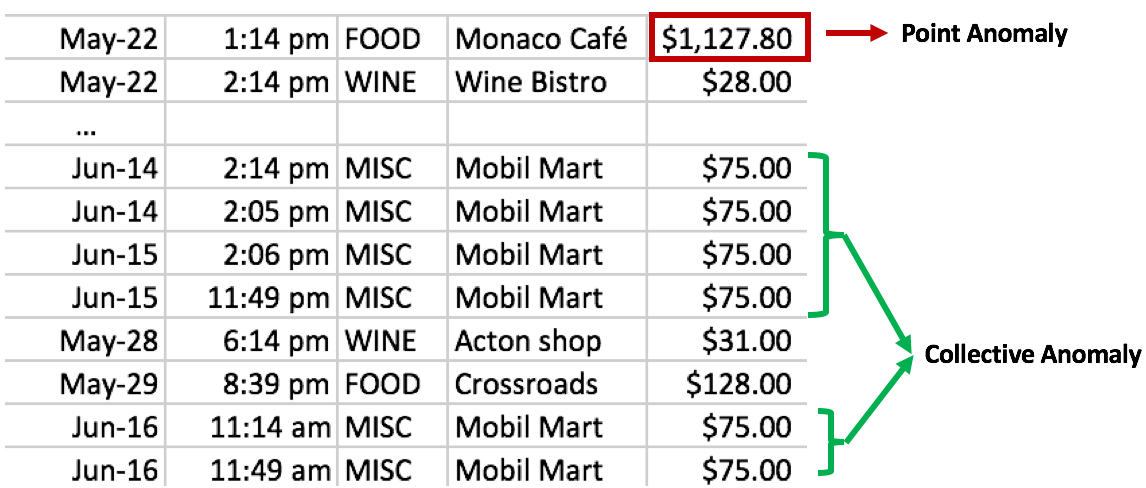
\includegraphics[scale=0.5]{images/PointAndCollectiveAnomaly}
\captionsetup{justification=centering}
\caption{Credit Card Fraud Detection: Illustrating Point and Collective anomaly.}
\label{fig:PointAndCollectiveAnomaly}
\end{figure}
%%%%%%%%%%%%%%%%%%%%%%%% End  Type of Anomalies %%%%%%%%%%%%%%%%%%%%%%%%


% Collective anomaly is also known as  group anomaly. While each individual data instances of this group may not be an anomaly, but their occurrence together as a collection is anomalous.

% Output of deep learning based anomaly detection methods
\subsection {Output of DAD Techniques}
\label{output_of_dad_methods}
An critical aspect for anomaly detection methods is the way in which the anomalies are identified. Generally, the outputs produced by anomaly detection methods are either anomaly score or binary labels.

\subsubsection{Anomaly Score:}
 Anomaly score describes the level of \textit{outlierness} for  each datapoint. The data instances may be ranked according to  anomalous score, and a domain specific threshold (commonly known as decision score) will be selected by subject matter expert to identify the anomalies.  In general, decision scores reveal more information than binary labels. In Deep SVDD approach the decision score is the measure of distance of data point from center of the sphere, the data points which are farther away from center are considered anomalous.

\subsubsection{Labels:} Instead of assigning scores, some techniques may assign a category label as normal or anomalous to each data instance. Unsupervised anomaly detection techniques using autoencoders measure  the magnitude of residual vector (i,e reconstruction error) for obtaining anomaly scores, later on the reconstruction errors are either ranked or thresholded by domain experts to label data instances.
%%%%%%%%%%%%%%%%%%%%%%%% End  Output of deep learning based AD %%%%%%%%%%%%%%%%%%%%%%%%


%!TEX root = ../main.tex
\section{Applications of Deep Anomaly Detection}
\label{sec:applicationsOfDLAD}

In this section we discuss several applications of deep anomaly detection. For each application
domain we discuss the following four aspects:\\
\textemdash the notion of anomaly;\\
\textemdash nature of the data;\\
\textemdash challenges associated with detecting anomalies;\\
\textemdash existing deep anomaly detection techniques.\\

%!TEX root = ../../main.tex
\subsection{Intrusion Detection}
\label{sec:intrusion_detection}

Intrusion detection  system (IDS) refers to identifying malicious activity in a computer related system~\cite{phoha2002internet}. IDS may be deployed at single computers known as Host Intrusion Detection (HIDS) to large networks Network Intrusion Detection (NIDS). The classification of deep anomaly detection techniques for intrusion detection is in Figure ~\ref{sec:intrusionDetect}. IDS depending on detection method are classified into signature based or anomaly based. Using signature based IDS is not efficient to detect new attacks, for which no specific signature pattern is available, hence anomaly based detection methods are more popular. In this survey we focus on deep anomaly detection (DAD) methods and architectures eemployed in intrusion detection.

\subsubsection{Host-Based Intrusion Detection Systems (HIDS):}
 Such systems are installed software programs which monitors a single host or computer for malicious  activity or policy violations by listening to system calls or events occurring within that host ~\cite{vigna2005host}. The system call logs could be generated by programs or by user interaction resulting in logs as shown in Figure~\ref{fig:deeplogContextual}. Malicious interactions lead to execution of these system calls in different sequences. HIDS may also monitor the state of a system, its stored information, whether in Random Access Memory (RAM), in the file system, log files or elsewhere for a valid sequence, hence the length of the sequence for each program may be different.
 Deep anomaly detection (DAD) techniques applied for HIDS are required to handle the sequential nature of data. The DAD techniques have to either model the sequence data or compute similarity between sequences. Some of the successfull DAD techniques for HIDS is illustrated in Table~\ref{tab:HIDS}.

\subsubsection{Network Intrusion Detection Systems (NIDS):} NIDS systems deal with monitoring the entire network for suspicious traffic by examining each and every network packet. Owing to real-time streaming behaviour, the nature of data is synomynous to big data with high volume, velocity, variety. The network data also has a temporal aspect associated with it. Some of the successfull DAD techniques for NIDS is illustrated in Table~\ref{tab:NIDS}. This survey also lists the datasets used for evaluating the DAD intrusion detection methods proposed in Table~\ref{tab:IDSDataset}. A challenge faced by deep anomaly detection techniques in intrusion detection is that the nature of anomalies keeps changing over time as the intruders adapt their network attacks to evade the existing intrusion detection solutions.

% Begin Figure
\begin{figure*}
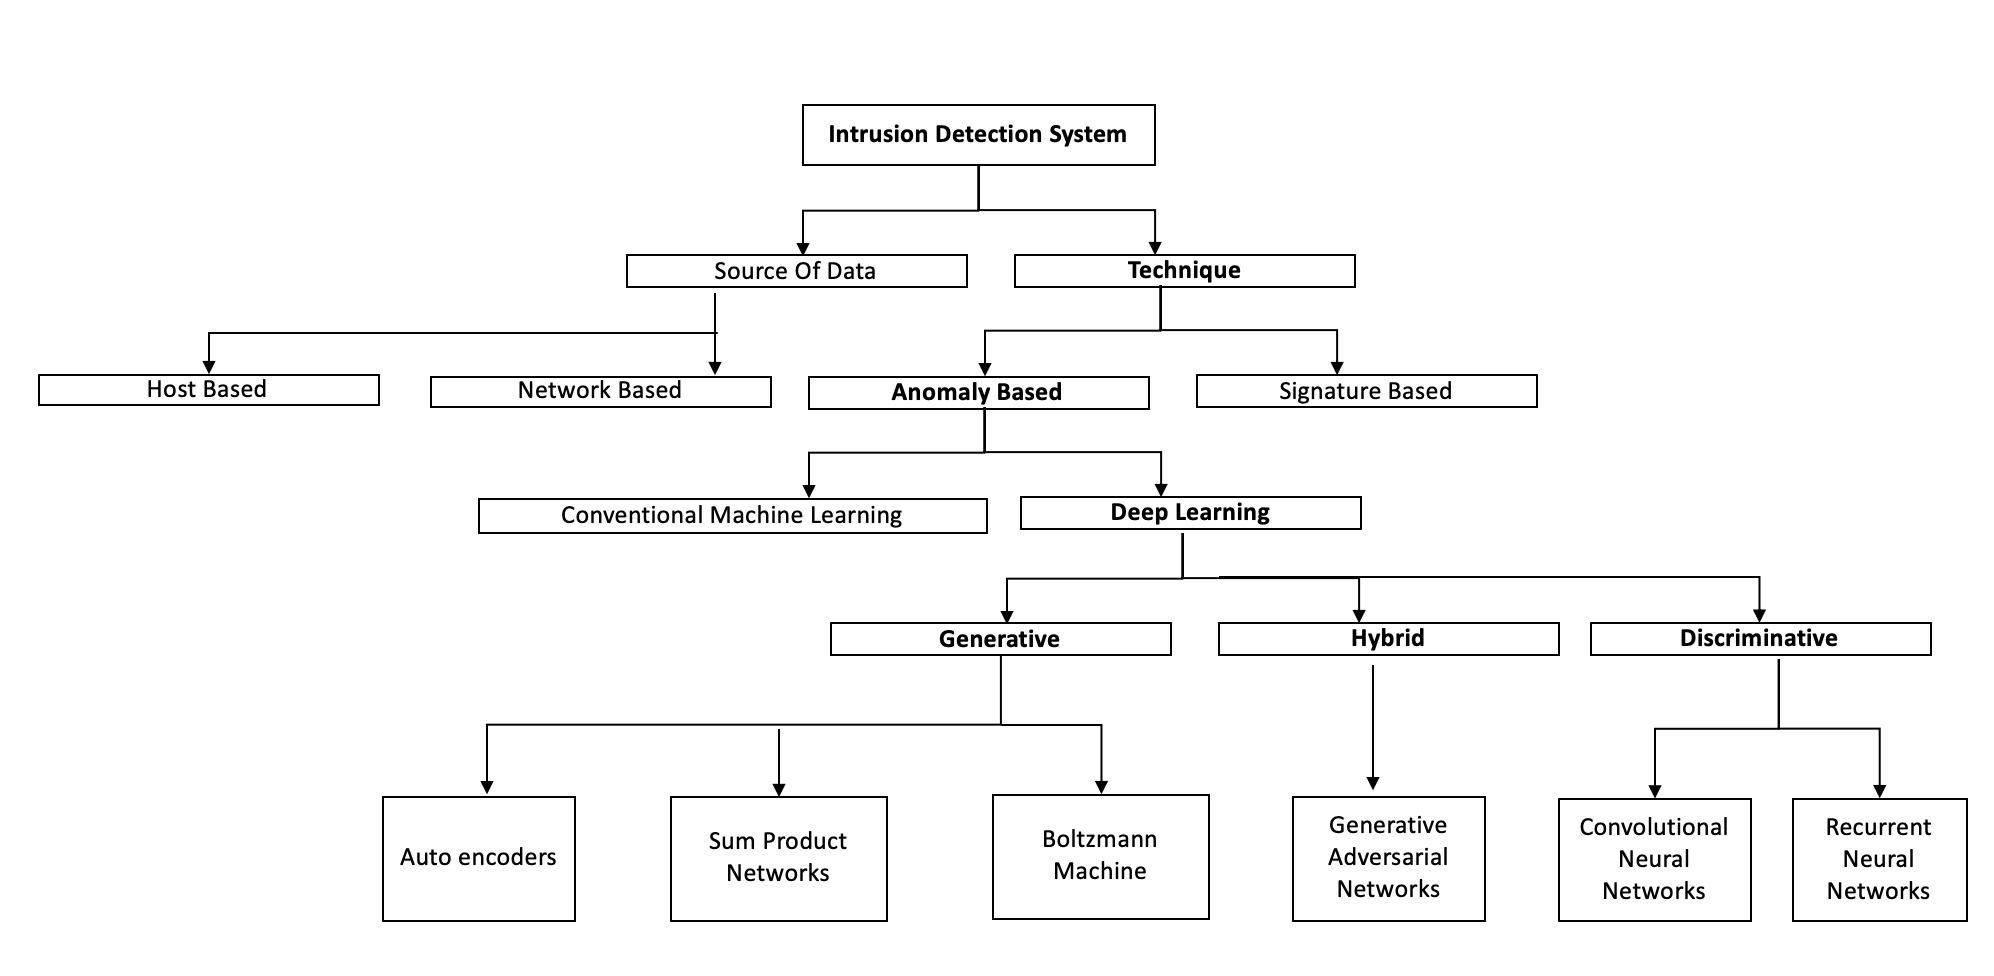
\includegraphics[scale=0.5]{images/IDS}
\captionsetup{justification=centering}
\caption{Classification of deep learning methods for Intrusion Detection.}
\label{fig:deepADforIDS}
\end{figure*}
% End of Figure


%%%%%%% HIDS Network intrusion detection%%%%%%%
%%% Table  Describing the model architectures and techniques used  of HIDS
\begin{table*}
\begin{center}
\caption{Examples of Deep learning anomaly detection Techniques Used in HIDS
          \\CNN: Convolution Neural Networks, LSTM : Long Short Term Memory Networks
          \\GRU: Gated Recurrent Unit, DNN : Deep Neural Networks
          \\SPN: Sum Product Networks}
  \label{tab:HIDS}
    \begin{tabular}{ | l | p{4cm} | l | p{5cm} |}
    \hline
    Techniques & Model Architecture & Section & References \\ \hline
    Discriminative &  LSTM , CNN-LSTM-GRU, DNN & Section ~\ref{sec:rnn_lstm_gru},~\ref{sec:cnn},~\ref{sec:dnn} &  ~\cite{kim2016lstm},~\cite{chawla2018host},~\cite{chen2018henet},~\cite{sohi2018recurrent},~\cite{vinayakumar2017applying} \\\hline
    Hybrid &  GAN & Section ~\ref{sec:hybridModels} & ~\cite{aghakhani2018detecting}, ~\cite{li2018anomaly} \\\hline
    Generative &  AE, SPN,  & Section ~\ref{sec:ae},~\ref{sec:spn} & ~\cite{gao2014intrusion},~\cite{peharz2018probabilistic},~\cite{umer2018two} \\
    \hline
    \end{tabular}
\end{center}
\end{table*}
%%%% End of Table NIDS




%%% Host based Intrusion detection system table%%%%%%
%%% Table  Describing the model architectures and techniques used  of NIDS
\begin{table*}
\begin{center}
  \caption{Examples of Deep learning anomaly detection Techniques Used in NIDS.
          \\CNN: Convolution Neural Networks, LSTM : Long Short Term Memory Networks
          \\RNN: Recurrent Neural Networks, RBM : Restricted Boltzmann Machines
          \\DCA: Dilated Convolution Autoencoders, CVAE : Convolutional Variational Autoencoder
          \\AE: Autoencoders, SAE: Stacked Autoencoders , DBN : Deep Belief Network
          \\GAN: Generative Adversarial Networks. }
  \label{tab:NIDS}
    \begin{tabular}{ | l | p{4cm} | l | p{5cm} |}
    \hline
    Techniques & Model Architecture & Section & References \\ \hline
   Generative  & DCA, SAE, RBM, DBN, CVAE & Section ~\ref{sec:cnn},~\ref{sec:ae},~\ref{sec:dnn},~\ref{sec:gan_adversarial} & ~\cite{yu2017network},~\cite{thing2017ieee}, ~\cite{zolotukhin2016increasing},~\cite{cordero2016analyzing},~\cite{alrawashdeh2016toward},~\cite{tang2016deep},~\cite{lopez2017conditional},~\cite{al2018deep},~\cite{mirsky2018kitsune},~\cite{aygun2017network} \\ \hline
  Hybrid  & GAN   & Section ~\ref{sec:hybridModels} & ~\cite{lin2018idsgan},~\cite{yin2018enhancing}, ~\cite{ring2018flow}, ~\cite{latah2018deep},~\cite{intrator2018mdgan},~\cite{matsubara2018anomaly},~\cite{nicolau2016hybrid} ,~\cite{rigaki2017adversarial}. \\ \hline
  Discriminative &  RNN , LSTM ,CNN & Section ~\ref{sec:rnn_lstm_gru},Section ~\ref{sec:cnn} & ~\cite{yu2017network}, ~\cite{malaiya2018empirical} ~\cite{kwon2018empirical},~\cite{gao2014intrusion},~\cite{staudemeyer2015applying},~\cite{naseer2018enhanced}\\
  \hline
  \end{tabular}
\end{center}
\end{table*}
%%%% End of Table NIDS


% Datasets Used Table
%%% Host based Intrusion detection system table%%%%%%
%%% Table  Describing the model architectures and techniques used  of NIDS
\begin{table*}
\begin{center}
  \caption{Datasets Used in Intrusion Detection }
   \label{tab:IDSDataset}
    \begin{tabular}{ | p{3cm} | l | p{5cm} | l | p{5cm} |}
    \hline
    DataSet &IDS & Description & Type & References \\ \hline
    CTU-UNB & NIDS & CTU-UNB~\cite{ucsdAnomalyDetect2017} dataset consists of various botnet traffics from CTU-13 dataset [20] and normal traffics from the UNB ISCX IDS 2012 dataset ~\cite{shiravi2012toward}  & Hexadecimal & ~\cite{yu2017network} \\ \hline
    Contagio-CTU-UNB & NIDS  & Contagio-CTU-UNB dataset consists of six types of network traffic data. ~\cite{adam2008robust}  & Text & ~\cite{yu2017network}. \\ \hline
    NSL-KDD~\footnote{http://nsl.cs.unb.ca/NSL-KDD/}& NIDS &The NSL-KDD data set is a refined version of its predecessor KDD‟99 data set.  ~\cite{ucsdAnomalyDetect2017} & Text &  ~\cite{yin2017deep},~\cite{javaid2016deep},  ~\cite{tang2016deep},~\cite{yousefi2017autoencoder},~\cite{mohammadi2017new}, ~\cite{lopez2017conditional}\\\hline
    DARPA KDD- CUP 99 & NIDS & DARPA KDD~\cite{stolfo2000cost} The competition task was to build a network intrusion detector, a predictive model capable of distinguishing between ``bad'' connections, called intrusions or attacks, and ``good'' normal connections.  & Text   & ~\cite{alrawashdeh2016toward} ,~\cite{van2017anomaly},~\cite{mohammadi2017new}\\\hline
    MAWI& NIDS  & The  MAWI~\cite{fontugne2010mawilab}  dataset  consists  of  network  traffic  capturedfrom  backbone  links  between  Japan  and  USA.  Every  daysince  2007  & Text   & ~\cite{cordero2016analyzing} \\\hline
    Realistic Global Cyber Environment (RGCE) & NIDS & RGCE~\cite{jamkRGCE}  contains
    realistic Internet Service Providers (ISPs) and numerous different web services as
    in the real Internet.  &  Text   & ~\cite{zolotukhin2016increasing} \\\hline
    ADFA-LD& HIDS & The ADFA Linux Dataset (ADFA-LD). This dataset provides a contemporary Linux dataset for evaluation by traditional HIDS~\cite{creech2014semantic} & Text   & ~\cite{kim2016lstm},~\cite{chawla2018host} \\\hline
    UNM-LPR& HIDS & Consists of system calls to evalute HIDS system~\cite{ImmuneDatasets} & Text   & ~\cite{kim2016lstm} \\\hline
    Infected PDF samples& HIDS & Consists of set of Infected PDF samples, which are used to monitor the malicious traffic  & Text   &~\cite{chen2018henet}\\\hline
    \end{tabular}
\end{center}
\end{table*}
%%%% End of Table NIDS













\label{sec:intrusionDetect}

%!TEX root = ../../main.tex
\subsection{Fraud Detection}
Fraud is a deliberate act of deception to access valuable resources~\cite{abdallah2016fraud}. The PwC global economic crime survey of 2018~\cite{Lavion2018,zhao2013fraud} found that half of the 7,200 companies they surveyed had experienced fraud of some nature. Fraud detection refers to detection of unlawfull activities across various industries, illustrated in Figure ~\ref{fig:AerasOfFraud}.

%%%%% Figure
\begin{figure}[h]
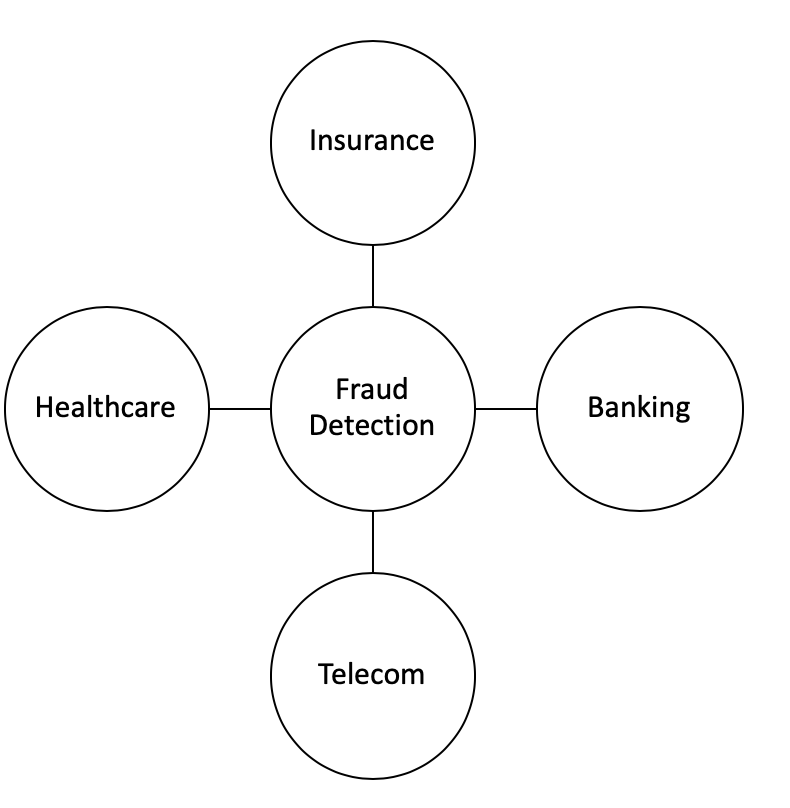
\includegraphics[scale=0.5]{images/AreasOfFraud}
\captionsetup{justification=centering}
\caption{Fraud detection across various application domains.}
\label{fig:AerasOfFraud}
\end{figure}
%%%%%%

Fraud in Telecom, insurance \textit{( health, automobile, etc)} claims, banking \textit{( tax return claims, credit card transactions etc)} represent significant problems in both governments and private businesses. Detecting and preventing fraud is not a simple task since fraud is an adaptive crime. Many traditional machine learning algorithms have been applied successfully in fraud detection~\cite{sorournejad2016survey}.  The challenge associated with detecting fraud is that it requires real time detection and prevention. This section focuses on deep anomaly detection (DAD) techniques for fraud detection.
%-----------------------------------------------------------------------------------------------------------

\subsubsection{Banking fraud:}
In the past decade, credit card was introduced in the banking sector. Now, credit card has become a popular
payment method in online shopping for goods and services. Credit card fraud involves theft of a payment card details, and use it as a fraudulent source of funds in a transaction. Many techniques for credit card fraud detection have been presented in the last few years~\cite{zhou2018state},~\cite{suganya2015survey}. Owing to the popularity of deep learning in various fields many techniques using deep learning models are proposed.
The challenge in credit card fraud detection is that frauds have no constant patterns. The typical approach in credit card fraud detection is to maintain a usage profile for each user and monitor the user profiles to detect any deviations. Since there are billions of credit card users this technique of user profile approach is not very scalabale. We will briefly review some of DAD techniques as shown Table~\ref{tab:creditfraudDetect}.
%%%%%%% Begin table fraud detection
\begin{table*}
\begin{center}
  \caption{Examples of Deep learning anomaly detection Techniques Used for credit card fraud detection.
          \\AE: Autoencoders, LSTM : Long Short Term Memory Networks
          \\RBM: Restricted Botlzmann Machines, DNN : Deep Neural Networks
          \\GRU: Gated Recurrent Unit, RNN: Recurrent Neural Networks
          \\CNN: Convolutional Neural Networks,VAE: Variational Autoencoders
          \\GAN: Generative Adversarial Networks}
  \label{tab:creditfraudDetect}
    \begin{tabular}{ | l | p{2cm} | p{7cm} |}
    \hline
    Technique Used & Section & References \\ \hline
     AE  & Section ~\ref{sec:ae}  & ~\cite{schreyer2017detection},~\cite{wedge2017solving} ,~\cite{paula2016deep},~\cite{renstrom2018fraud},~\cite{kazemi2017using},~\cite{zheng2018one},~\cite{pumsirirat2018credit} \\\hline
     RBM  & Section ~\ref{sec:dnn}  & ~\cite{pumsirirat2018credit} \\\hline
     DBN & Section ~\ref{sec:dnn} & ~\cite{seeja2014fraudminer} \\\hline
     VAE & Section ~\ref{sec:gan_adversarial} & ~\cite{sweers2018autoencoding} \\\hline
     GAN & Section ~\ref{sec:gan_adversarial} & ~\cite{fiore2017using},~\cite{choi2018generative} \\\hline
     DNN  & Section ~\ref{sec:dnn} & ~\cite{dorronsoro1997neural}, ~\cite{gomez2018end} \\\hline
     LSTM,RNN,GRU  & Section ~\ref{sec:rnn_lstm_gru} & ~\cite{wiese2009credit}, ~\cite{jurgovsky2018sequence} ,~\cite{heryadi2017learning},~\cite{ando2016detecting},~\cite{wang2017session},~\cite{alowais2012credit},~\cite{amarasinghe2018critical},~\cite{abroyan2017neural},~\cite{lp2018transaction}\\\hline
     CNN  & Section ~\ref{sec:cnn} & ~\cite{shen2007application},~\cite{chouiekh2018convnets},~\cite{abroyan2017convolutional},~\cite{fu2016credit},~\cite{lu2017deep},~\cite{wang2018credit},~\cite{abroyan2017neural} ,~\cite{zhang2018model}\\\hline
    \end{tabular}
\end{center}
\end{table*}
%%%%%%%%% End of table Banking detection




%-----------------------------------------------------------------------------------------------------------
\subsubsection{Mobile cellular network fraud:}
In recent times, mobile cellular networks  have witnessed  rapid deployment and evolution
supporting billions of users and a vast diverse array of mobile devices.
Due to this wide adoption and low mobile cellular service rates mobile
cellular networks is now faced with frauds such as voice scams targeted to steal customer private information, and messaging related scams to extort money from customers. Detecting such fraud is of paramount interest and not an easy task due to volume and velocity of mobile cellular network.
Traditional machine learning methods with static feature engineering  techniques fail to adapt to the nature of evolving fraud.
Table ~\ref{tab:mobilefraudDetect} lists DAD techniques for mobile cellular network fraud detection.

%%%%%%% Begin table fraud detection
\begin{table*}
\begin{center}
  \caption{Examples of Deep learning anomaly detection Techniques Used for mobile cellular network fraud detection.
          \\CNN:  convolution neural networks,DBN: Deep Belief Networks
          \\SAE: Stacked Autoencoders, DNN : Deep neural networks
          \\GAN: Generative Adversarial Networks }
  \label{tab:mobilefraudDetect}
    \begin{tabular}{ | l | p{2cm} | l | p{5cm} |}
    \hline
    Technique Used & Section & References \\ \hline
     CNN    & Section ~\ref{sec:cnn}  & ~\cite{chouiekh2018convnets} \\\hline
     SAE, DBN    & Section \ref{sec:ae}, Section ~\ref{sec:dnn}   &  ~\cite{alsheikh2016mobile},~\cite{badhe2017click} \\\hline
     DNN & Section ~\ref{sec:dnn}  &  ~\cite{akhter2012detecting},~\cite{jain2017perspective} \\\hline
     GAN & Section ~\ref{sec:gan_adversarial} &  ~\cite{zheng2018generative} \\\hline
    \end{tabular}
\end{center}
\end{table*}
%%%%%%%%% End of table fraud detection
%-----------------------------------------------------------------------------------------------------------
\subsubsection{Insurance fraud:}
Several traditional machine learning methods have been applied successfully to detect fraud in insurance claims ~\cite{joudaki2015using,roy2017detecting}. The traditional approach for fraud detection is based on features which are fraud indicators. The challenge with the traditional approaches is that the need of manual expertise. Another challenge is insurance fraud detection is the that the incidence of frauds is far less than the total number of claims, and also each fraud is unique in its own way. In order to overcome these limitations several deep anomaly detection techniques are proposed which are illustrated in Table ~\ref{tab:insurancefraudDetect}

%%%%%%% Begin table fraud detection
\begin{table*}
\begin{center}
  \caption{Examples of Deep learning anomaly detection Techniques Used for insurance fraud detection.
          \\DBN: Deep Belief Networks, DNN : Deep Neural Networks
          \\CNN: Convolutional Neural Networks,VAE: Variational Autoencoders
          \\GAN: Generative Adversarial Networks}
  \label{tab:insurancefraudDetect}
    \begin{tabular}{ | l | p{2cm} | l | p{5cm} |}
    \hline
     DBN & Section ~\ref{sec:dnn} & ~\cite{viaene2005auto} \\\hline
     VAE & Section ~\ref{sec:gan_adversarial} & ~\cite{fajardo2018vos} \\\hline
     GAN & Section ~\ref{sec:gan_adversarial} & ~\cite{fiore2017using},~\cite{choi2018generative} \\\hline
     DNN & Section ~\ref{sec:dnn} &~\cite{keung2009neural}\\\hline
     CNN  & Section ~\ref{sec:cnn} & ~\cite{shen2007application},~\cite{zhang2018model}\\\hline
    \end{tabular}
\end{center}
\end{table*}
%%%%%%%%% End of Insurance fraud
% \ref{sec:dnn}
% \ref{sec:stn}
% \ref{sec:spn}
% \ref{sec:word2vec}
% \ref{sec:gan_adversarial}
% \ref{sec:cnn}
% \ref{sec:rnn_lstm_gru}
% \ref{sec:ae}
%-----------------------------------------------------------------------------------------------------------
\subsubsection{Health insurance fraud:}

Healthcare is an integral component in people's lives, waste, abuse and fraud drive up costs in healthcare by tens of billions of dollars each year. Healthcare insurance claims fraud is a major contributor to increased healthcare costs, but its impact can be mitigated through fraud detection. Several machine learning models have been used effectively in health care insurance fraud~\cite{bauder2017medicare}.
This section presents the overview of deep learning based anomaly detection methods for healthcare fraud identification.
%%%%%%% Begin table fraud detection
\begin{table*}
\begin{center}
  \caption{Examples of Deep learning anomaly detection Techniques Used for health care fraud detection.
          \\RBM: Restricted Botlzmann Machines, GAN: Generative Adversarial Networks}
  \label{tab:healthcarefraudDetect}
    \begin{tabular}{ | l | p{2cm} | l | p{5cm} |}
    \hline
    Technique Used & Section & References \\ \hline
     RBM & Section ~\ref{sec:dnn} & ~\cite{lasaga2018deep} \\\hline
     GAN & Section ~\ref{sec:gan_adversarial} & ~\cite{ghasedi2018semi},~\cite{finlayson2018adversarial}\\\hline
     CNN  & Section ~\ref{sec:cnn} & ~\cite{esteva2017dermatologist}\\\hline
    \end{tabular}
\end{center}
\end{table*}
%%%%%%%%% End of table health care fraud

%-----------------------------------------------------------------------------------------------------------

\label{sec:fraudDetection}

%!TEX root = ../../main.tex
\subsection{Malware Detection}

Malware, short for Malicious Software. In  order to protect legitimate users from malware, machine learning based efficient malware detection  methods are proposed ~\cite{ye2017survey}. In these classical machine learning methods, the process of detection is usually divided into two stages: feature extraction and classification/clustering. The performance of traditional malware detection approaches critically depend on the extracted features and the methods for classification/clustering. The challenge associated in malware detection problems is the seer scale of data, for instance considering data as bytes a certain  sequence classification problem could be  of the order of two million time steps. The  malware is very adpative in nature, the attackers use advanced techniques to hide the malicious behaviour. Some anomaly detection techniques for malware detection is shown in Table ~\ref{tab:malwareDetect}.

\begin{table*}
  \begin{center}
   \caption{Examples of Deep learning anomaly detection Techniques Used for malware detection.
             \\AE: Autoencoders, LSTM : Long Short Term Memory Networks
             \\RBM: Restricted Botlzmann Machines, DNN : Deep Neural Networks
             \\GRU: Gated Recurrent Unit, RNN: Recurrent Neural Networks
             \\CNN: Convolutional Neural Networks,VAE: Variational Autoencoders
             \\GAN: Generative Adversarial Networks,CNN-BiLSTM: CNN- Bidirectional LSTM}
    \label{tab:malwareDetect}
    \begin{tabular}{l|c|p{7cm}}
      \textbf{Technique Used} & \textbf{Section} & \textbf{References}\\
      \hline
      AE &  Section ~\ref{sec:ae}  & ~\cite{yousefi2017autoencoder},~\cite{hardy2016dl4md},~\cite{yousefi2017autoencoder},~\cite{de2018malware},~\cite{sewak2018investigation},~\cite{kebede2017classification},~\cite{de2018malware},~\cite{david2015deepsign}\\\hline
      word2vec & Section ~\ref{sec:word2vec} &  ~\cite{cakir2018malware},~\cite{silva2018improving}\\\hline
      CNN & Section ~\ref{sec:cnn} &  ~\cite{kolosnjaji2018adversarial},~\cite{suciu2018exploring},~\cite{srisakaokul2018muldef},~\cite{srisakaokul2018muldef},~\cite{king2018artificial},~\cite{huang2017r2},~\cite{guo2017malware},~\cite{abdelsalam2018malware},~\cite{raff2017malware},~\cite{karbab2018maldozer},~\cite{martinelli2017evaluating},~\cite{mclaughlin2017deep},~\cite{gibert2018using},~\cite{kolosnjaji2017empowering}\\\hline
      DNN & Section ~\ref{sec:dnn} &  ~\cite{rosenberg2018end},~\cite{wang2017adversary}\\\hline
      DBN & Section ~\ref{sec:dnn} &  ~\cite{david2015deepsign},~\cite{yang2016application},~\cite{ding2016application},~\cite{yuxin2017malware},~\cite{selvaganapathy2018deep},~\cite{yuxin2017malware},~\cite{hou2017deep}\\\hline
      LSTM & Section ~\ref{sec:rnn_lstm_gru} &  ~\cite{tobiyama2016malware}, ~\cite{hu2017black},~\cite{tobiyama2018method} ,~\cite{passalislong} \\\hline
      CNN-BiLSTM& Section ~\ref{sec:cnn},~\ref{sec:rnn_lstm_gru} &  ~\cite{le2018deep},~\cite{wang2017adversary} \\\hline
      GAN& Section ~\ref{sec:gan_adversarial} &  ~\cite{kim2018zero} \\\hline
      Hybrid model(AE + CNN), (AE + DBN) & Section ~\ref{sec:hybridModels} &  ~\cite{wang2018effective},~\cite{li2015hybrid} \\\hline
      RNN & Section ~\ref{sec:rnn_lstm_gru} &  ~\cite{haddadpajouh2018deep} \\\hline

    \end{tabular}
  \end{center}
\end{table*}



% OCSVM~\cite{scholkopf2002support}, SVDD~\cite{scholkopf2002support}
% SVM~\cite{cortes1995support}
% KNN~\cite{altman1992introduction}
% Random Forest~\cite{ho1995random}
% Relief~\cite{kira1992feature}
% CSI~\cite{ruchansky2017csi}
% \ref{sec:dnn}
% \ref{sec:stn}
% \ref{sec:spn}
% \ref{sec:word2vec}
% \ref{sec:gan_adversarial}
% \ref{sec:cnn}
% \ref{sec:rnn_lstm_gru}
% \ref{sec:ae}





\label{sec:malwareDetection}

%!TEX root = ../../main.tex
\subsection{Medical Anomaly Detection:}
\label{sec:medical_anomaly_detection}

 A survey of theoretical and practical aspects of deep learning in medical and bioinformatics is described by ~\cite{min2017deep,cao2018deep,zhao2016deep,khan2018review}. Finding rare objects and events (anomalies) in areas such as medical image analysis, Clinical electroencephalography (EEG) records which consists of vast amounts of complex data enables to diagnose and provide preventive treatments for a variety of medical conditions. Deep learning based architectures are employed with great success as illustrated in Table ~\ref{tab:medicalanomalyDetect}. The vast amount of imbalanced data in medical domain presents significant challenges anomaly detection. Additionally deep learning techniques for long have been considered as black-box techniques, i,e even though deep learning models produce outstanding performance, these models lack interpretability. In recent times these works by ~\cite{gugulothusparse,amarasinghe2018toward,choi2018doctor} demonstrate models with good interpretability and performance.
%%%%%%% Begin table fraud detection
\begin{table*}
\begin{center}
  \caption{Examples of Deep learning anomaly detection Techniques Used for medical anomaly detection.
          \\AE: Autoencoders, LSTM : Long Short Term Memory Networks
          \\GRU: Gated Recurrent Unit, RNN: Recurrent Neural Networks
          \\CNN: Convolutional Neural Networks,VAE: Variational Autoencoders
          \\GAN: Generative Adversarial Networks, KNN: K-nearest neighbours
          \\RBM: Restricted Boltzmann Machines.}
  \label{tab:medicalanomalyDetect}
    \begin{tabular}{ | l | p{4cm} | p{7cm} |}
    \hline
    Technique Used & Section & References \\ \hline
     AE  & Section~\ref{sec:ae} & ~\cite{wang2016research,cowton2018combined},~\cite{sato2018primitive}\\\hline
     DBN & Section~\ref{sec:dnn} & ~\cite{turner2014deep},~\cite{sharma2016abnormality},~\cite{wulsin2010semi},~\cite{ma2018unsupervised},~\cite{zhang2016automatic},~\cite{wulsin2011modeling} ,~\cite{wu2015adaptive}\\\hline
     RBM & Section~\ref{sec:dnn}  & ~\cite{liao2016enhanced}\\\hline
     VAE & Section~\ref{sec:gan_adversarial} & ~\cite{xu2018unsupervised},~\cite{lu2018anomaly} \\\hline
     GAN & Section~\ref{sec:gan_adversarial}&~\cite{ghasedi2018semi},~\cite{chen2018unsupervised} \\\hline
     LSTM ,RNN,GRU & Section~\ref{sec:rnn_lstm_gru} & ~\cite{yang2018toward},~\cite{jagannatha2016bidirectional},~\cite{cowton2018combined},~\cite{o2016recurrent},~\cite{latif2018phonocardiographic},~\cite{zhang2018time},~\cite{chauhan2015anomaly},~\cite{gugulothusparse,amarasinghe2018toward}\\\hline
     CNN  & Section~\ref{sec:cnn} & ~\cite{schmidt2018artificial},~\cite{esteva2017dermatologist},~\cite{wang2016research},~\cite{iakovidis2018detecting}\\\hline
     Hybrid( AE+ KNN) & Section~\ref{sec:cnn} & ~\cite{song2017hybrid} \\\hline
    \end{tabular}
\end{center}
\end{table*}
%%%%%%%%% End of table Medical anomaly detection








\label{sec:medicalAnomalyDetect}


%!TEX root = ../../main.tex
\subsection{Deep learning for Anomaly detection in Social Networks}
In recent times, online social networks has become part and parcel of daily life. Anomalies in social network
are irregular often unlawfull behaviour pattern of individuals within a social network, such  individuals may be identified as  spammers, sexual predators, online fraudsters, fake users or rumour-mongers. Detecting these irregular patterns is of prime importance since if not detected, the act of such indivuals can have serious social impact. A survey of classical anomaly detection techniques in social networks is presented by ~\cite{savage2014anomaly,anand2017anomaly,yu2016survey,cao2018automatic,yu2016survey}.
Besides the challenges of classical anomaly detection ~\cite{liu2017social} tasks, social network anomaly detection lead to new challenges due to  heterogeneous and dynamic nature of data. In this section we review the deep anomaly models used for anomaly detection in social networks as illustrated in Table ~\ref{tab:socialNetworkAnomalyDetect}.

% Table
\begin{table*}
  \begin{center}
   \caption{Examples of Deep learning anomaly detection techniques used to detect anomalies in social network.
            \\CNN: Convolution Neural Networks, LSTM : Long Short Term Memory Networks
            \\AE: Autoencoders, DAE: Denoising Autoencoders
            \\SVM : Support Vector Machines., DNN : Deep Neural Network  }
    \label{tab:socialNetworkAnomalyDetect}
    \begin{tabular}{l|p{4cm}|p{5cm}}
      \textbf{Technique Used} & \textbf{Section} & \textbf{References}\\
      \hline
      AE,DAE &  Section ~\ref{sec:ae}  & ~\cite{zhang2017detecting},~\cite{castellini2017fake}\\\hline
      CNN-LSTM & Section ~\ref{sec:cnn}, ~\ref{sec:rnn_lstm_gru} & ~\cite{sun2018detecting},~\cite{shu2017doc},~\cite{yang2018anomaly}\\\hline
      DNN & Section ~\ref{sec:dnn}  & ~\cite{li2017detecting}\\\hline
      Hybrid Models (CNN-LSTM-SVM) & Section ~\ref{sec:hybridModels}  & ~\cite{wei2017new}\\\hline
    \end{tabular}
  \end{center}
\end{table*}





% Science is a belief in the ingnorance of experts
% Measure of ignorance; Data Artist
% Find Worst Case: Piano
%New Ideas in Business and Intelligence and customer analytics
%Learn the rules like a professional but break like an artist

\label{sec:socialNetworks}


%!TEX root = ../../main.tex
\subsection{Log Anomaly Detection:}
Anomaly detection in log file aims to find text which can indicate the reasons and the nature of failure of a system. Most commonly, a domain  specific regular-expression  is contructed from past experience which finds new faults by pattern matching, the limitation of such approach is that newer messages of failures are easily are not detected~\cite{memon2008log}. The unstructured and diversity in both format and semantics of log data pose significant challenges to anomaly detection. Futhermore log data is produced in real time with large volume and speed, hence anomaly detection techniques should adapt to this concurrent setting and detect outliers in real time  in order to be useful so that users can take appropriate actions. Following the success of deep neural networks in text analysis in real time, several deep anomaly detection (DAD) techniques are proposed to detect outliers in log data as illustrated in Table~\ref{tab:logAnomalyDetect}. DAD methods model system log as a natural language sequence.


%%%%%%% Begin table fraud detection
\begin{table*}
\begin{center}
\caption{Examples of Deep learning anomaly detection Techniques Used in system logs.
        \\CNN: Convolution Neural Networks, LSTM : Long Short Term Memory Networks
        \\GRU: Gated Recurrent Unit, DNN : Deep Neural Networks
        \\AE: Autoencoders, DAE: Denoising Autoencoders}
  \label{tab:logAnomalyDetect}
    \begin{tabular}{ | l | p{2cm} | p{6cm} |}
    \hline
     \textbf{Techniques}  & \textbf{Section} & \textbf{References} \\ \hline
     LSTM & Section ~\ref{sec:rnn_lstm_gru} & ~\cite{hochreiter1997long},~\cite{brown2018recurrent},~\cite{tuor2017deep},~\cite{das2018desh},~\cite{malhotra2015long} \\\hline
     AE & Section ~\ref{sec:ae} & ~\cite{du2017deeplog},~\cite{andrews2016detecting} ,~\cite{sakurada2014anomaly},~\cite{nolle2018analyzing},~\cite{nolle2016unsupervised}\\\hline
     LSTM-AE & Section ~\ref{sec:rnn_lstm_gru}, ~\ref{sec:ae} & ~\cite{grover2018anomaly},~\cite{wolpher2018anomaly} \\\hline
     RNN & Section ~\ref{sec:rnn_lstm_gru} & ~\cite{brown2018recurrent},~\cite{zhang2018role},~\cite{nanduri2016anomaly},~\cite{fengming2017anomaly}\\\hline
     DAE & Section ~\ref{sec:ae} & ~\cite{marchi2015non},~\cite{nolle2016unsupervised}\\\hline
     CNN & Section ~\ref{sec:cnn} & ~\cite{lu2018detecting},~\cite{yuan2018insider},~\cite{racki2018compact},~\cite{zhou2016spatial},~\cite{gorokhov2017convolutional},~\cite{liao2017deep},~\cite{cheng2017deep},~\cite{zhang2018alphamex}\\\hline
    \end{tabular}
\end{center}
\end{table*}
%%%%%%%%% End of Log anomaly detection











\label{sec:logAnomaly}


%!TEX root = ../../main.tex
\subsection{Internet of things (IoT) Big Data Anomaly Detection}

IoT is identified as a network of  devices that is interconnected with softwares, servers, sensors and etc. In the field of Internet of things (IoT), data generated by weather stations, RFID tags, IT infrastructure
components, and some other sensors are mostly time series sequential data. Anomaly detection in these IoT networks identifies fraudulent, faulty behaviour of these massive scale of interconnected devices. The challenges associated  in outlier detection is that heterogeneous devices are interconnected which renders the system more complex. A thorough overview on using  deep learning (DL), to facilitate the analytics and learning in the IoT domain is presented by ~\cite{mohammadi2018deep}. In this section we present some of the deep anomaly detection techniques used in this domain in Table ~\ref{tab:iotBigDataAnomalyDetect}.

%%%%%%% Begin table iot BigData Anomaly Detect
\begin{table*}
\begin{center}
\caption{Examples of Deep learning anomaly detection Techniques Used in Internet of things (IoT) Big Data Anomaly Detection.
        \\ AE: Autoencoders, LSTM : Long Short Term Memory Networks
        \\ DBN : Deep Belief Networks.}
  \label{tab:iotBigDataAnomalyDetect}
    \begin{tabular}{ | l | p{2cm} | p{6cm} |}
    \hline
     \textbf{Techniques}  & \textbf{Section} & \textbf{References} \\ \hline
     AE & Section ~\ref{sec:ae} & ~\cite{luo2018distributed},~\cite{mohammadi2018neural} \\\hline
     DBN & Section ~\ref{sec:dnn} & ~\cite{kakanakova2017outlier} \\ \hline
     LSTM & Section ~\ref{sec:rnn_lstm_gru} & ~\cite{zhang2018lstm},~\cite{mudassar2018unsupervised}\\ \hline
    \end{tabular}
\end{center}
\end{table*}
%%%%%%%%% End of iot BigData Anomaly Detect






\label{sec:iotBigDataAnomaly}

%!TEX root = ../../main.tex
\subsection{Industrial Anomalies Detection}

Industrial systems consisting of wind turbines, power plants, high-temperature energy systems, storage devices and  with rotating mechanical parts are exposed to enormous stress on a day-to-day basis. Damage to these type of systems not only causes economic loss but also a loss of reputation, therefore detecting and repairing them early is of utmost importance. Several machine learning techniques have been used to detect such damage in industrial systems ~\cite{ramotsoela2018survey,marti2015anomaly}, following the recent success of deep learning several papers published utilizing deep learning models show great promise~\cite{atha2018evaluation,de2018automatic,wang2018residential}. Damages caused to equipments are rare events, thus  detecting such events can be formulated as outlier detection problem. The challenges associated with outlier detection in this domain is both volume as well as dynamic nature of data, since failure can be caused due to variety of factors. Some deep anomaly detection techniques employed across various industries are shown in Table ~\ref{tab:industrialDamageDetect}.



%%%%%%% Begin table industrial damage detection
\begin{table*}
\begin{center}
\caption{Examples of Deep learning anomaly detection Techniques Used in industrial operations.
        \\CNN: Convolution Neural Networks, LSTM : Long Short Term Memory Networks
        \\GRU: Gated Recurrent Unit, DNN : Deep Neural Networks
        \\AE: Autoencoders, DAE: Denoising Autoencoders, SVM: Support Vector Machines
        \\SDAE: Stacked Denoising Autoencoders, RNN : Recurrent Neural Networks.}
    \label{tab:industrialDamageDetect}
    \begin{tabular}{ | l | p{2cm} | p{6cm} |}
    \hline
     \textbf{Techniques}  & \textbf{Section} & \textbf{References} \\ \hline
     LSTM & Section ~\ref{sec:rnn_lstm_gru} &  ~\cite{inoue2017anomaly},~\cite{thi2017one},~\cite{kravchik2018detecting},~\cite{huang2018deep},~\cite{park2018lired},~\cite{chang2018review}\\\hline
     AE & Section ~\ref{sec:ae} & ~\cite{yuan2015distributed},~\cite{araya2017ensemble},~\cite{qu2017detection},~\cite{sakurada2014anomaly},~\cite{bhattad2018detecting}\\\hline
     DNN & Section ~\ref{sec:dnn} & ~\cite{lodhi2017power}\\\hline
     CNN & Section ~\ref{sec:cnn} & ~\cite{faghih2016deep},~\cite{christiansen2016deepanomaly},~\cite{lee2016convolutional},~\cite{faghih2016deep}, ~\cite{dong2016camera},~\cite{nanduri2016anomaly},~\cite{fuentes2017robust},~\cite{huang2018deep},~\cite{chang2018review}\\\hline
     SDAE,DAE & Section ~\ref{sec:ae} & ~\cite{yan2015accurate},~\cite{luo2017gas},~\cite{dai2017cleaning} \\\hline
     RNN & Section ~\ref{sec:rnn_lstm_gru} & ~\cite{banjanovic2017neural},~\cite{thi2017one} \\\hline
     Hybrid Models (DNN-SVM) & Section ~\ref{sec:hybridModels} & ~\cite{inoue2017anomaly} \\\hline
    \end{tabular}
\end{center}
\end{table*}
%%%%%%%%% End of industrial damage detection












\label{sec:industrialDamageDetect}

%!TEX root = ../../main.tex
\subsection{Anomaly Detection in Time Series }
\label{sec:timeseriesAD}
Data recorded continuously over a duration is known the time series. A review of Deep learning methods to classify , detect anomalies is presented by ~\cite{fawaz2018deep,langkvist2014review,gamboa2017deep,lu2017unsupervised}. Time series data are the best examples of collective outliers. Furthermore DeepAD, an anomaly detection framework to detect anomalies precisely, even in complex data patterns is proposed by~\cite{buda2018deepad}. With the increase of time series data (sensor data) availability, many deep models are explored and are shown to produce good results in outlier detection. Some of the challenges to detect anomalies in time series using deep learning models data are:
\begin{itemize}
    \item Lack of defined pattern in which an anomaly occuring may be defined.
    \item Noise present seriously effects the performance of algorithms.
    \item As the Length of the time series data increases the computational complexity also increases.
    \item Deep learning models should be able to detect anomalies in real time.
    \item  Time series data is usually non-stationary, non-linear and dynamically evolving.
\end{itemize}
Recent advancements in the deep learning domain offer
opportunities to extract rich hierarchical features which can greatly improve outlier detection as illustrated by various techniques shown in Table ~\ref{tab:sensorAnomalyDetect}.

%%%%%%% Begin table sensor networks time series anomaly detection
\begin{table*}
\begin{center}
\caption{Examples of Deep learning anomaly detection Techniques Used in time series data.
        \\CNN: Convolution Neural Networks, GAN: Generative Adversarial networks,LSTM : Long Short Term Memory Networks
        \\GRU: Gated Recurrent Unit, DNN : Deep Neural Networks,
        \\AE: Autoencoders, DAE: Denoising Autoencoders, VAE: Variational Autoencoder
        \\ SDAE: Stacked Denoising Autoencoders}
  \label{tab:sensorAnomalyDetect}
    \begin{tabular}{ | l | p{2cm} | p{6cm} |}
    \hline
    \textbf{Techniques}  & \textbf{Section} & \textbf{References} \\ \hline
     LSTM & Section ~\ref{sec:rnn_lstm_gru} &  ~\cite{shipmon2017time},~\cite{hundman2018detecting},~\cite{zhu2017deep},~\cite{hundman2018detecting},~\cite{malhotra2015long},~\cite{chauhan2015anomaly},~\cite{assendorp2017deep},~\cite{buda2018deepad},~\cite{ahmad2017unsupervised},~\cite{malhotra2016lstm},~\cite{bontemps2016collective},~\cite{taylor2016anomaly},~\cite{cheng2016ms},~\cite{loganathan2018sequence},~\cite{chauhan2015anomaly},\cite{malhotra2015long},~\cite{gorokhov2017convolutional}\\\hline
     AE,LSTM-AE,CNN-AE,GRU-AE & Section ~\ref{sec:ae} & ~\cite{Dominique},~\cite{kieu2018outlier},~\cite{cowton2018combined},~\cite{malhotra2016multi},~\cite{malhotra2016lstm},~\cite{filonov2016multivariate},~\cite{sugimoto2018deep},~\cite{oh2018residual},~\cite{ebrahimzadehmulti}\\\hline
     RNN & Section ~\ref{sec:rnn_lstm_gru} & ~\cite{wielgosz2017recurrent},~\cite{saurav2018online},~\cite{wielgosz2018model},~\cite{guo2016robust}\\\hline
     CNN, CNN-LSTM & Section ~\ref{sec:cnn},~\ref{sec:rnn_lstm_gru} & ~\cite{kanarachos2017detecting},~\cite{dumodeling},~\cite{gorokhov2017convolutional},~\cite{napoletano2018anomaly},~\cite{shanmugam2018jiffy},\cite{medel2016anomaly}\\\hline
     LSTM-VAE & Section ~\ref{sec:rnn_lstm_gru},~\ref{sec:gan_adversarial} & ~\cite{park2018multimodal},~\cite{solch2016variational}\\\hline
     DNN &Section ~\ref{sec:dnn} & ~\cite{amarasinghe2018toward}\\\hline
     GAN &Section ~\ref{sec:gan_adversarial} & ~\cite{li2018anomaly},~\cite{zenati2018efficient},~\cite{lim2018doping},~\cite{laptevanogen}\\\hline
    \end{tabular}
\end{center}
\end{table*}
%%%%%%%%% End of time series anomaly detection




\label{sec:sensorNetworkAnomaly}


%!TEX root = ../../main.tex
\subsection{Video Surveillance}
Video Surveillance also popularly known as Closed-circuit television (CCTV) involves monitoring a designated areas of interest in order to ensure security. In Videos surveillance applications unlabelled data is available in large amounts, this is a significant challenge for supervised machine learning and deep learning methods. Also in literature videos surveillance applications have been modelled as anomaly detection problems owing to lack of availability of labelled data. ~\cite{kiran2018overview,chong2015modeling} reviews the state-of-the-art deep learning based methods for video anomaly detection and categorizes them based on the type of model and criteria of detection. The challenges of robust 24/7 video surveillance systems is discussed in detail by ~\cite{boghossian2005challenges}. In addition to those challenges lack of  explicit definition of anomaly in real-life video surveillance is a significant issue that hampers the performance of deep anomaly detection methods as well. A few deep anomaly detection (DAD) techniques used in  video surveillance  are illustrated  in Table ~\ref{tab:sensorAnomalyDetect}.

%%%%%%% Begin table for video survellienace anomaly detection
\begin{table*}
\begin{center}
\caption{Examples of Deep learning anomaly detection Techniques Used in video surveillance.
        \\CNN: Convolution Neural Networks, LSTM : Long Short Term Memory Networks
        \\RBM: Restricted Boltzmann Machine, DNN : Deep Neural Networks, CAE: Convolutional Autoencoders
        \\AE: Autoencoders, DAE: Denoising Autoencoders, OCSVM: One class Support vector machines
        \\SDAE: Stacked Denoising Autoencoders, STN : Spatial Transformer Networks }
  \label{tab:videoSurvellianceAnomalyDetect}
    \begin{tabular}{ | l | p{4cm} | p{6cm} |}
      \hline
      \textbf{Technique Used} & \textbf{Section} & \textbf{References}\\
      \hline
      CNN & Section ~\ref{sec:cnn}   & ~\cite{dong2016camera}, ~\cite{andrewsaanomaly}, ~\cite{sabokrou2016fully}~\cite{sabokrou2017deep},~\cite{munawar2017spatio},~\cite{li2017transferred},~\cite{qiao2017abnormal},~\cite{tripathi2018convolutional},~\cite{nogas2018deepfall},~\cite{christiansen2016deepanomaly},~\cite{li2017transferred}\\\hline
      SAE (AE + CNN-LSTM)  &  Section ~\ref{sec:ae},~\ref{sec:cnn},~\ref{sec:rnn_lstm_gru}  & ~\cite{chong2017abnormal},~\cite{qiao2017abnormal},~\cite{khaleghi2018improved}\\\hline
      AE &  Section ~\ref{sec:ae}  & ~\cite{qiao2017abnormal},~\cite{yang2015unsupervised},~\cite{chen2015detecting},~\cite{gutoskidetection},~\cite{d2017autoencoder},~\cite{dotti2017unsupervised},~\cite{yang2015unsupervised},~\cite{chen2015detecting},~\cite{sabokrou2016video},~\cite{tran2017anomaly},~\cite{chen2015detecting} ,~\cite{d2017autoencoder},~\cite{hasan2016learning},~\cite{yang2015unsupervised},~\cite{cinelli2017anomaly}\\\hline
      Hybrid Model (CAE-OCSVM) & Section ~\ref{sec:hybridModels}  & ~\cite{gutoskidetection}, ~\cite{dotti2017unsupervised}\\\hline
      LSTM-AE &  Section ~\ref{sec:rnn_lstm_gru}, ~\ref{sec:ae}  & ~\cite{d2017autoencoder}\\\hline
      STN &Section~\ref{sec:stn}   & ~\cite{chianucci2016unsupervised}\\\hline
      RBM &Section ~\ref{sec:dnn}   & ~\cite{munawar2017spatio}\\\hline
      LSTM &Section ~\ref{sec:rnn_lstm_gru}  &~\cite{medel2016anomaly},~\cite{luo2017remembering},~\cite{ben2018attentioned},~\cite{singh2017anomaly}\\\hline
      RNN & Section ~\ref{sec:rnn_lstm_gru} &~\cite{luo2017revisit},~\cite{zhou2015abnormal} ,~\cite{hu2016video},~\cite{chong2015modeling}\\\hline
      AAE & Section ~\ref{sec:gan_adversarial} & ~\cite{ravanbakhsh2017training}\\\hline
    \end{tabular}
  \end{center}
\end{table*}
%%%%%%%%% End of video survellienace anomaly detection





% % Datasets Used Table
% \begin{table*}
%   \begin{center}
%     \caption{Datasets Used For Video surveillance}
%     \label{tab:videoSurvelliance}
%     \begin{tabular}{|p{3cm}|p{4cm}|p{6cm}|}
%       \hline
%       \textbf{DataSet} & \textbf{Type} & \textbf{References}\\
%       \hline
%       UCSD Ped2~\cite{ucsdAnomalyDetect2017},Subway~\cite{adam2008robust} &  Video   & Sabokrou et al~\cite{sabokrou2016fully,sabokrou2017deep}, Gutoski et al~\cite{gutoskidetection} \\ \hline
%       LOST ~\cite{Abrams et al. 2012} &  Video   & Dotti et al~\cite{dotti2017unsupervised}\\ \hline
%       YouTube &  Video   & Yang et al~\cite{yang2015unsupervised}\\ \hline
%       UMN~\footnote{$http://mha.cs.umn.edu$} &  Video   & Sabokrou et al~\cite{yang2015unsupervised}\\ \hline
%       CIFAR-10 &Images& Munawar et al~\cite{munawar2017spatio} \\ \hline
%     \end{tabular}
%   \end{center}
% \end{table*}
% %%%%%%%%% End of Datasets used in video survellienace anomaly detection



































\label{sec:videoSurvelliance}












%!TEX root = ../main.tex
\section{Deep Anomaly Detection (DAD) Models}
\label{sec:deepDADModels}

In this section we discuss various deep anomaly detection based on training objective. For each model types domain we discuss the following four aspects:\\
\textemdash assumptions;\\
\textemdash type of model architectures;\\
\textemdash computational complexity;\\
\textemdash advantages and disadvantages;\\

%!TEX root = ../../main.tex
\subsection{Supervised Deep Anomaly Detection}
\label{sec:supervisedDAD}
~\cite{gornitz2013toward} argue that supervised anomaly detection techniques are superior in performance compared to  unsupervised learning techniques since these techniques leverage labeled samples and depend on discriminating data classes. Supervised anomaly detection illustrated in Section~\ref{supervised_learning} is used to learn a model (classifier) from a set of labeled data instances (training) and then, classify a test instance into one of the classes using the learnt model (testing).\\
\textbf{Assumptions :} \\
Supervised learning methods depend on separating data classes whereas unsupervised
techniques focus on explaining and understanding the characteristics of data. A supervised classifier based on the labels available for training phase, can be grouped into two broad categories: multi-class and semi-supervised discussed in Section ~\ref{semi_supervised_DAD}. Multi-class classification based anomaly detection techniques assume that the training data contains labeled instances of  multiple normal classes ~\cite{shilton2013combined,jumutc2014multi,kim2015deep,erfani2017shared}. Multi-class anomaly detection techniques learn a classifier to distinguish between each normal class against the rest of the classes. In general, supervised deep learning-based classification schemes for anomaly detection have two subnetworks, a feature extraction network followed by a classifier network. Deep models  requires the availability of multiple classes for training and extremely large number of training samples (in the order of thousands or millions) to effectively learn feature representations to discriminate various class instances. Due to, lack of availability of clean data labels supervised deep anomaly detection techniques are not so popular as semi-supervised and unsupervised methods.

\textbf{Computational Complexity :} \\
The computational complexity of supervised deep anomaly detection methods based techniques depends on the dimensionality of the input data. High dimensional data tend to have more hidden layers to ensure meaningfull hierarchical learning of input features. As the number of hidden layers of deep learning networks increases, the computational complexity also increases accordingly, which increases the model training and update time.


\textbf{Advantages and Disadvantages of Classification Based Techniques :}\\
The advantages of supervised deep anomaly detection techniques are as follows:
\begin{itemize}
\item Supervised deep anomaly detection techniques, especially the multi-class techniques, can make
use of powerful algorithms that can distinguish between instances belonging to
different classes.\\
\item The testing phase of classification based techniques is fast since each test instance
needs to be compared against the pre-computed model.
\end{itemize}
The disadvantages of classification based techniques are as follows:
\begin{itemize}
\item  Multi-class supervised techniques require accurate labels for various normal classes, which is often not available.
\item Supervised techniques fail to separate normal from anomalous data , if the feature space is highly complex and non-linear.
\end{itemize}













\label{sec:supervised}

%!TEX root = ../../main.tex
\subsection{Semi-supervised Deep Anomaly Detection (DAD)}
\label{sec:semi_supervised_DAD}
Semi-supervised or (one-class classification) deep anomaly detection techniques assume that all training instances have only one class label.  A review of deep learning based semi-supervised techniques is presented by ~\cite{kiran2018overview,min2018ids}. Such techniques learn a discriminative boundary around the normal instances using a one-class classification algorithm,
.The test instance that does not belong within the learnt boundary is flagged as anomalous
~\cite{perera2018learning,blanchard2010semi}.
Benefiting from the ability of nonlinear feature learning abililty of deep models, the DAE is trained to learn features of a high-dimensional dataset, these features are then input to nonparametric KNN-based anomaly detectors~\cite{song2017hybrid}. These hybrid  architectures are a promising technique for learning robust features using deep learning model and input to traditional classifier algorithms. Various deep semi-supervised model architectures employed for anomaly detection are illustrated in Table~\ref{tab:semisupervisedModels}.

%%%%%%% Begin table Semi-supervised deep anomaly detection models
\begin{table*}
\begin{center}
\caption{Semi-supervised deep anomaly detection models overview
        \\AE: Autoencoders, DAE: Denoising Autoencoders, KNN : K- Nearest Neighbours
        \\CorGAN: Corrupted Generative Adversarial Networks, DBN: Deep Belief Networks
        \\ AAE: Adversarial Autoencoders, CNN: Convolution neural networks
        \\ SVM:  Support vector machines.}
    \label{tab:semisupervisedModels}
    \begin{tabular}{ | p{4cm} | p{2cm} | p{4cm} |}
    \hline
     \textbf{Techniques}  & \textbf{Section} & \textbf{References} \\ \hline
     AE & Section ~\ref{sec:ae} & ~\cite{edmunds2017deep} ,~\cite{estiri2018semi}\\\hline
     RBM & Section ~\ref{sec:dnn} & ~\cite{jia2014novel} \\\hline
     DBN & Section ~\ref{sec:dnn} & ~\cite{wulsin2010semi},~\cite{wulsin2011modeling} \\\hline
     CorGAN,GAN & Section~\ref{sec:gan_adversarial} & ~\cite{gu2018semi} ~\cite{akcay2018ganomaly},~\cite{sabokrou2018adversarially}\\\hline
     AAE &Section~\ref{sec:gan_adversarial} & ~\cite{dimokranitou2017adversarial}\\\hline
     Hybrid Models (DAE-KNN~\cite{altman1992introduction}), (DBN-Random Forest~\cite{ho1995random}),CNN-Relief~\cite{kira1992feature},CNN-SVM~\cite{cortes1995support} & Section~\ref{sec:gan_hybridModels} & ~\cite{song2017hybrid},~\cite{shi2017semi},~\cite{zhu2018hybrid} \\\hline
     CNN & Section~\ref{sec:cnn} & ~\cite{racah2017extremeweather},~\cite{perera2018learning} \\ \hline
     RNN & Section~\ref{sec:rnn_lstm_gru} & ~\cite{wu2018semi} \\ \hline
     GAN & Section~\ref{sec:gan_adversarial} & ~\cite{kliger2018novelty},~\cite{gu2018semi} \\ \hline
    \end{tabular}
\end{center}
\end{table*}
%%%%%%%%% End of industrial damage detection

% OCSVM~\cite{scholkopf2002support}, SVDD~\cite{scholkopf2002support}
% SVM~\cite{cortes1995support}
% KNN~\cite{altman1992introduction}
% Random Forest~\cite{ho1995random}
% Relief~\cite{kira1992feature}
% CSI~\cite{ruchansky2017csi}
% Section ~\ref{sec:ae}
% Section ~\ref{sec:rnn_lstm_gru}
% Section ~\ref{sec:gan_adversarial}
% Section ~\ref{sec:dnn}
% Section ~\ref{sec:cnn}
% Section ~\ref{sec:hybridModels}


\textbf{Assumptions : } \\
In semi-supervised learning settings most of the algorithms proposed rely on one the following assumptions to score a data instance as an anomaly.
\begin{itemize}
 \item  Proximity and Continuity: Points which are close to each other both in input space  and learnt feature space are more likely to share a same label.
  \item Robust features are extracted within deep neural network layers, which aid in separating normal from outlier data points.
\end{itemize}

\textbf{Computational Complexity :} \\
The computational complexity of semi-supervised deep anomaly detection methods based techniques is same as supervised deep anomaly detection techniques, which primarily depends on the dimensionality of the input data and the number of hidden layers used for representative feature learning.

\textbf{Advantages and Disadvantages of Classification Based Techniques :}\\
The advantages of semi-supervised deep anomaly detection techniques are as follows:
\begin{itemize}
\item Semi-supervised deep anomaly detection techniques, are widely deployed since cost associated with obtaining labelled data is very high and infeasible sometimes. Generative Adversarial Networks (GANs) trained in semi-supervised learning mode have shown great promise, even with very few labeled data.
\item  It has been shown that the use of labeled data ( usually of one class), can produce considerable improvement in performance  accuracy over unsupervised techniques.
\end{itemize}
The fundamental disadvantages of semi-supervised techniques discussed in ~\cite{lu2009fundamental} holds good even in deep learning context. Additionally the points to consider are as follows.
\begin{itemize}
\item  Deep semi-supervised models are also prone to overfitting, due to lack of labeled instances of other class.
\item The hierarchical features extracted within hidden layers may not be representative of fewer anomalous instances since, these deep learning based models require large amount of data instances  to learn good discriminative features.
\end{itemize}










\label{sec:semiSupervised}

%!TEX root = ../../main.tex
\subsection{Hybrid Deep Anomaly Detection (DAD) Models}
\label{sec:hybridModels}
The hidden layer representation of deep learning models  has been utilized  for choosing features, to best support outlier detection~\cite{andrews2016detecting}. Feeding these hidden representations into traditional algorithms like one-class Radial Basis Function (RBF) , Support Vector Machine (SVM) classifiers forms a new class Hybrid models ~\cite{erfani2016high,erfani2016robust,wu2015harvesting} that are shown to produce good results. The Table ~\cite{tab:hybridModels} illustrates the list of Hybrid models utilized for anomaly detection.

%%%%%%% Begin table industrial damage detection
\begin{table*}
\begin{center}
\caption{Examples of  Hybrid Deep learning anomaly detection Techniques.
        \\CNN: Convolution Neural Networks, LSTM : Long Short Term Memory Networks
        \\DBN: Deep Belief Networks, DNN : Deep Neural Networks.
        \\AE: Autoencoders, DAE: Denoising Autoencoders, SVM: Support Vector Machines
        \\SVDD: Support Vector Data Description, RNN : Recurrent Neural Networks
        \\Relief: Feature selection Algorithm, KNN: K- Nearest Neighbours
        \\CSI: Capture, Score, and Integrate. }
    \label{tab:hybridModels}
    \begin{tabular}{ | p{3cm} | p{2cm} | p{6cm} |}
    \hline
     \textbf{Techniques}  & \textbf{Section} & \textbf{References} \\ \hline
     AE-OCSVM, AE-SVM & 21D & ~\cite{andrews2016detecting} \\\hline
     DBN-SVDD, AE-SVDD & 21D & ~\cite{erfani2016high},~\cite{kim2015deep} \\\hline
     DNN-SVM & 21D & ~\cite{inoue2017anomaly} \\\hline
     DAE-KNN, DBN-Random Forest,CNN-Relief,CNN-SVM & 21D & ~\cite{song2017hybrid},~\cite{shi2017semi},~\cite{zhu2018hybrid,urbanowicz2018relief} \\\hline
     AE-CNN, AE-DBN & Section 7.1.2 &  ~\cite{wang2018effective},~\cite{li2015hybrid} \\\hline
     AE+ KNN & 21B & ~\cite{song2017hybrid} \\\hline
     CNN-LSTM-SVM & Section 7.2.1  & ~\cite{wei2017new}\\
     RNN-CSI & Section 7.2.1  & ~\cite{ruchansky2017csi}\\
     CAE-OCSVM &  Section 7.2.X  & ~\cite{gutoskidetection}, ~\cite{dotti2017unsupervised}\\\hline
    \end{tabular}
\end{center}
\end{table*}
%%%%%%%%% End of Hybrid Models

\textbf{Assumptions : } \\
The deep hybrid models proposed for anomaly detection rely on one the following assumptions to detect outliers:
\begin{itemize}
 \item  Hybrid models tend to perform better on on complex, highdimensional datasets since traditional non-parametric learning models such as SVMs,complexity grows quadratically with the number of records.
  \item Robust features are extracted within hidden layers of deep neural network, which aid in separating out the irrelevant features which can conceal the presence of anomalies.
  \item Building a robust anomaly detection model in complex, high-dimensional spaces needs both an unsupervised feature extractor and an anomaly detector. Various anomaly detectors used alongwith are illustrated in Table ~\cite{tab:hybridModels}
\end{itemize}

\textbf{Computational Complexity :} \\
Computational complexity of an hybrid model includes complexity of both deep architectures as well as traditional algorithms used within. The deeper models tend to perform better,if the individual layers are pre-trained ~\cite{saxe2011random} which introduces computational expenditure. Additionally  an inherent issue of non-trivial choice of deep network architecture and parameters which involves searching optimized parameters in a considerably larger space introduces the computational complexity of using deep layers within hybrid models. Furthermore considering the classical algorithms such as  linear SVM which has prediction complexity  of $O(d)$ with d the number of input dimensions. For most kernels, including polynomial and RBF, the complexity is $O(nd)$ where $n$ is the number of support vectors although an approximation $O(d^2)$ is considered for SVMs with an RBF kernel.

\textbf{Advantages and Disadvantages of Classification Based Techniques :}\\
The advantages of semi-supervised deep anomaly detection techniques are as follows:
\begin{itemize}
\item  A promising technique for learning robust features, and can greatly reduce the ‘curse of dimensionality’ especially in high dimensional domain.
\item  Linear or nonlinear kernel models may be used to utilize the rich features extracted rending the model more scalable and computationally efficient.
\end{itemize}
The significant disadvantages of hybrid techniques for anomaly detection are:
\begin{itemize}
\item  The hybrid approach of learning deep features using an deep neural network and then feeding the features into a separate anomaly detection method like one-class SVM (OC-SVM) is suboptimal because it is unable to influence representational learning in the hidden layers.
\item  Although using generic pre-trained networks for transfer learning representations is efficient, learning representations from scratch, on a moderately sized dataset, for a specific task of anomaly detection is shown to perform better~\cite{andrews2016transfer}.
\end{itemize}













\label{sec:hybrid}

%!TEX root = ../../main.tex
\subsection{One class Neural Networks (OC-NN) for Anomaly Detection}
\label{sec:oneclassNN}
The One class Neural Networks  (OC-NN) combines the ability of deep networks to extract progressively rich representation of data alongwith the one-class objective, such as an hyperplane~\cite{chalapathy2018anomaly} or hypersphere ~\cite{ruff2018deep} to separate all the normal data points from the origin. The OC-NN approach is novel for the following crucial reason: data representation in the hidden layer as illustrated in
The experimental results in ~\cite{chalapathy2018anomaly,ruff2018deep} demonstrate that OC-NN can achieve comparable or better performance than existing state-of-the art methods for complex datasets, while having reasonable training and testing time compared to the existing methods.

\textbf{Assumptions : } \\
The OC-NN models proposed for anomaly detection rely on one the following assumptions to detect outliers:
\begin{itemize}
 \item  OC-NN models extracts the common factors of variation within the data distribution within the hidden layers of deep neural network to fit the model outputs into a hypersphere of minimum volume or construct a separating hyperplane.
  \item Performs combined representation learning and produces a outlier score for test data instance.
  \item Anomalous samples do not contain common factors of variation and hence hidden layers fails to capture the representations of outliers.
\end{itemize}

\textbf{Computational Complexity :} \\
The Computational complexity of an OC-NN model as against the  hybrid model includes only the complexity of deep network of choice ~\cite{saxe2011random}. OC-NN models do not require  data to be
stored for prediction, thus have very low memory complexity.However  it is evident that the OC-NN takes the longest time to train and is proportional to the dimension of the input space.

\textbf{Advantages and Disadvantages of OC-NN Techniques :}\\
The advantages of OC-NN deep anomaly detection techniques are as follows:
\begin{itemize}
\item  OC-NN  models jointly trains a deep neural network while optimizing a data-enclosing hypersphere or hyperplane in output space.
\item OC-NN~\cite{chalapathy2018anomaly} propose an alternating minimization algorithm for learning
the parameters of the OC-NN model. We observe that the subproblem of the OC-NN objective is equivalent to a solving a quantile selection problem which is well defined.
\end{itemize}
The significant disadvantages of OC-NN for anomaly detection are:
\begin{itemize}
\item Training times may be longer for high dimensional input data.
\item Model updates would also take longer time, given the change in input space.
\end{itemize}



\label{sec:oneClassNeuralNetworks}

%!TEX root = ../../main.tex
\subsection{Un-supervised Deep Anomaly Detection (UDAD)}
\label{sec:unsupervisedDAD}
Unsupervised anomaly detection is an important area of research  in both fundamental machine learning research and industrial applications. Several deep learning frameworks that addresses  challenges in unsupervised anomaly detection are proposed and shown to produce state-of-the-art performance as illustrated in Table ~\ref{tab:unsupervisedAnomalyDetection}. Autoencoders are the fundamental  unsupervised deep architectures used in anomaly detection~\cite{baldi2012autoencoders}.

%%%%%%% Begin Un-supervised Deep Anomaly Detection (UDAD)
\begin{table*}
\begin{center}
\caption{Examples of  Un-supervised Deep Anomaly Detection (UDAD).
        \\CNN: Convolution Neural Networks, LSTM : Long Short Term Memory Networks
        \\DNN : Deep Neural Networks., GAN: Generative Adversarial Network
        \\AE: Autoencoders, DAE: Denoising Autoencoders, SVM: Support Vector Machines
        \\STN: Spatial Transformer Networks, RNN : Recurrent Neural Networks
        \\AAE: Adversarial Autoencoders, VAE : Variational Autoencoders.}
    \label{tab:unsupervisedAnomalyDetection}
    \begin{tabular}{ | l | p{2cm} | p{6cm} |}
    \hline
     \textbf{Techniques}  & \textbf{Section} & \textbf{References} \\ \hline
     LSTM & Section ~\ref{sec:rnn_lstm_gru} &  ~\cite{singh2017anomaly},~\cite{chandola2008comparative},~\cite{dasigi2014modeling},\cite{malhotra2015long}\\\hline
     AE & Section ~\ref{sec:ae} & ~\cite{abati2018and},~\cite{zong2018deep},~\cite{tagawa2015structured},~\cite{dau2014anomaly},~\cite{sakurada2014anomaly},~\cite{wu2015adaptive},~\cite{xu2015learning},~\cite{hawkins2002outlier},~\cite{zhao2015robust},~\cite{qi2014robust},~\cite{chalapathy2017robust},~\cite{yang2015unsupervised},~\cite{zhai2016deep},~\cite{lyudchik2016outlier},~\cite{lu2017unsupervised},~\cite{mehrotra2017deep},~\cite{meng2018relational},\cite{parchami2017using}\\\hline
     STN & Section ~\ref{sec:stn} & ~\cite{chianucci2016unsupervised}\\\hline
     GAN & Section ~\ref{sec:gan_adversarial} & ~\cite{lawson2017finding} \\\hline
     RNN & Section ~\ref{sec:rnn_lstm_gru} & ~\cite{dasigi2014modeling},\cite{filonov2017rnn} \\\hline
     AAE & Section ~\ref{sec:gan_adversarial} & ~\cite{dimokranitou2017adversarial},~\cite{leveau2017adversarial} \\\hline
     VAE & Section ~\ref{sec:gan_adversarial} &  ~\cite{an2015variational},~\cite{suh2016echo},~\cite{solch2016variational},~\cite{xu2018unsupervised},~\cite{mishra2017generative}\\\hline
    \end{tabular}
\end{center}
\end{table*}
%%%%%%%%% End of Un-supervised Deep Anomaly Detection (UDAD)

% OCSVM~\cite{scholkopf2002support}, SVDD~\cite{scholkopf2002support}
% SVM~\cite{cortes1995support}
% KNN~\cite{altman1992introduction}
% Random Forest~\cite{ho1995random}
% Relief~\cite{kira1992feature}
% CSI~\cite{ruchansky2017csi}
% Section ~\ref{sec:ae}
% Section ~\ref{sec:rnn_lstm_gru}
% Section ~\ref{sec:gan_adversarial}
% Section ~\ref{sec:dnn}
% Section ~\ref{sec:cnn}
% Section ~\ref{sec:stn}
% Section ~\ref{sec:hybridModels}

\textbf{Assumptions : } \\
The deep unsupervised  models proposed for anomaly detection rely on one the following assumptions to detect outliers:
\begin{itemize}
 \item The “normal” regions in the original or some latent feature space can be distinguished from "anomalous" regions in the original or some latent feature space.
  \item The majority of the data instances are normal compared to the remainder of the data set.
  \item Unsupervised anomaly detection algorithm produces an outlier score of the data instances based on  intrinsic properties of the dataset such as distances or densities. The hidden layers of deep neural network aim to capture these intrinsic properties within the dataset~\cite{goldstein2016comparative}.
\end{itemize}

\textbf{Computational Complexity :} \\
The autoencoders is the most common architecture employed in outlier detection with quadratic cost, the optimization problem is non-convex in nature similar to any other neural network architecture.
The model computational complexity depends on the number of operations, network parameters and layers. However, the computational complexity of training an autoencoder is much higher than traditional methods such as Principal Component Analysis (PCA) since PCA is
based on matrix decomposition ~\cite{meng2018relational,parchami2017using}.\\
\textbf{Advantages and Disadvantages of unsupervised deep anomaly detection techniques :}
The advantages of unsupervised deep anomaly detection techniques are as follows:
\begin{itemize}
\item  Learns the inherent data characteristics to separate normal from anomalous data point. These technique  identifies commonalities within the data therefore facilitates outlier detection.
\item  Cost effective technique to find the anomalies since it does not require annotated data for training the algorithms.
\end{itemize}
The significant disadvantages of unsupervised deep anomaly detection techniques are:
\begin{itemize}
\item  Often it is difficult to learn commonalities within data in a complex and high dimensional space.
\item While using autoencoders the choice of right degree of compression, i.e. dimensionality reduction is often an hyper-parameter that requires tuning for optimal results.
\item Unsupervised techniques techniques are very sensitive to noise, and data corruptions and
       are often less accurate than supervised or semi-supervised techniques.
\end{itemize}









\label{sec:unsupervised}

%!TEX root = ../../main.tex
\subsection{Miscellaneous Techniques}
This section explores, different deep anomaly detection techniques which are shown to be effective and promising,  we discuss the key idea behind those techniques, and their area of applicability.

\subsubsection{Transfer Learning based anomaly detection : }
Deep learning for long has been critized for the need to have enough data to produce good results.
Transfer learning relaxes this data dependence which motivates one to use transfer learning
to solve the problem of insufficient training data. ~\cite{litjens2017survey,pan2010survey} present the review on deep transfer learning approaches. Transfer learning is an important tool in machine learning to solve the basic problem of insufficient training data. It aims to transfer the knowledge from the source domain to the target domain by relaxing the assumption that the training and future data must be in the same feature space and have the same distribution. Deep transfer representation-learning has been explored by ~\cite{andrews2016transfer,vercruyssen2017transfer,li2012detecting,almajai2012anomaly,kumar2017transfer,liang2018transfer} and shown to produce very promising results. The open research questions using transfer learning for anomaly detection is , the degree of  transferability, that is to define how well features at that layer transfer from one task to another. Obtaining greater understanding of these open questions could be a valuble resource for improving deep anomaly detection performance.

\subsubsection{Zero Shot learning based anomaly detection:}
Zero shot learning (ZSL)  aims recognize objects never seen before within training set~\cite{romera2015embarrassingly}.
ZSL achieves this  in two phases: Firstly the  knowledge about the objects in natural language descriptions or attributes (commonly known as meta-data) is captured Secondly this knowledge is then used to classify instances among a new set of classes. This setting is important in the real world since one may not be able to obtain images of all the possible classes at training. The main challenge associated with this approach is the obtaining the meta-data about the data instances. However several approaches of using ZSl in anomaly and novelty detection are shown to produce state-of-the-art results ~\cite{mishra2017generative,,socher2013zero,xian2017zero,liu2017generalized,rivero2017grassmannian}.

\subsubsection{Ensemble based anomaly detection:}
 A notable issue with deep neural networks is that they are sensitive to noise and often
require large training data to perform robustly. In order to achieve robustness even in noisy data an idea to randomly vary on the connectivity architecture of the autoencoder to obtain
signicantly better performance. An autoencoder ensembles consisting of  various randomly connected autoencoders are experimented by  ~\cite{chen2017outlier} to achieve promising results on several bench-mark datasets. Similarly ~\cite{kim2016lstm} employ a novel ensemble method that combines  multiple thresholding classifiers into a single one unit , enabling it possible to recognize ‘highly normal’ sequences. The ensemble approaches are still an active area of research which has been shown to produce improved diversity, thus avoiding overfitting and reducing the training time.

\subsubsection{Clustering based anomaly detection:}
Several anomaly detection  algorithms based on clustering have been proposed in literature ~\cite{ester1996density}. Clustering involves grouping together similar patterns based on features extracted  detect new anomalies.  Deep learning enabled clustering approach anomaly detection utilizes word2vec ~\cite{mikolov2013efficient}  models to get the semantical presentations of normal data and anomalies. Finally, the features extracted are grouped to form clusters and detect outliers ~\cite{yuan2017deep}. Many works rely on variants of hybrid models with auto-encoders and use the encoder outputs as representations for clustering ~\cite{aytekin2018clustering,xie2016unsupervised,guo2017improved,xie2016unsupervised,guo2017deep,wang2016learning,mani2018scalable}. The time and space complexity grows linearly with number of classes to be clustered ~\cite{sreekanth2010generalized}, which renders the clustering based anomaly detection prohibitive for real-time practical applications. The dimensionality of the data is reduced by using the extracted features within the hidden layers of deep neural network which ensures scalability for complex and high dimensional datasets.


\subsubsection{Deep Reinforcement Learning (DRL) based anomaly detection:}
\label{reinforcementlearning},
Deep reinforcement learning (DRL) methods have attracted significant interest due to its ability to learn complex behaviors in high-dimensional data space. Efforts to detect anomalies using deep reinforcement learning have been proposed by ~\cite{de2017learning,rlanomaly}.
The DRL based anomaly detector  does not consider any assumption about the concept of the anomaly,  the detector identifies new anomalies by consistently enhancing its knowledge  through reward signals accumulated. DRL based anomaly detection is a very novel concept which  requires identification of research gap and its applications.

\subsubsection{Statistical Techniques based anomaly detection: }
Hilbert transform is statistical signal processing technique which derives the analytic representation of a real-valued signal. This property is leveraged by ~\cite{kanarachos2015anomaly} for real time detection of anomalies health related time series dataset and is shown to be a very promising technique. The algorithm is expressed as a combination of wavelet analysis, neural networks and Hilbert transform in a sequential manner.  Although the authors claim the real time detection of anomalies In the fourth comming years these statistical signal processing techniques have been rarely experimented due to the fact that the training phase can be computationally demanding and exprensive.


\label{sec:others}

%!TEX root = ../main.tex
\section{Deep Neural Network Architectures for Locating Anomalies}
\label{sec:locatingAnomalieswithNNArchitecture}


\subsection{Deep Neural Networks}
\label{sec:dnn}
The "deep" in "deep neural networks" refers to the number of layers through which the features of data are extracted~\cite{schmidhuber2015deep,bengio2009learning}. Deep architectures overcome the limitations of traditional machine learning approaches of scalability, and generalization to new variations within data~\cite{lecun2015deep}. Deep Belief Networks (DBNs) are class of deep neural network which comprises of multiple layer of graphical models known as Restricted Boltzmann Machine (RBMs).
The hypothesis in using DBNs for anomaly detection is that RBMs are used as  directed encoder-decoder network that can be trained with backpropogation algorithm~\cite{werbos1990backpropagation}. DBNs fail to learn good representations of anomalous samples, resulting in high reconstruction error. DBNs  are shown to scale efficiently to a large training set and improve interpretability~\cite{wulsin2010semi}.


\subsection{Spatio Temporal Networks (STN)}
\label{sec:stn}
Researchers for long have explored  techniques to learn both both spatial and temporal relation features , since modeling local spatial temporal correlation has wide applications~\cite{zhang2018detecting}. Deep learning architectures have been shown perform well at learning spatial aspects ( using CNNs) and temporal features ( using LSTMs) individually. Spatio Temporal Networks (STNs) comprise of deep neural architectures combining both CNNs and LSTMs to extract spatio-temporal features. The temporal
features (modeling correlations between near time points via LSTM), spatial features (modeling
local spatial correlation via local CNNs) are shown to be effective in detecting outliers~\cite{lee2018stan,szeker2014spatio,nie2018spatio,dereszynski2011spatiotemporal}.

\subsection{ Sum-Product Networks (SPN)}
\label{sec:spn}
Sum-Product Networks (SPNs) are directed acyclic graphs with variables as leaves, while the internal nodes, and weighted edges constitute the sums and products. SPNs are considered as a combination of mixture models ~\cite{poon2011sum,peharz2018probabilistic} which have fast exact probabilistic inference over many layers. The main advantage of SPNs is that, unlike graphical models, SPNs are more traceable over high treewidth models without requiring approximate inference. Furthermore, SPNs are shown to capture uncertainty over their inputs in a convincing manner, yielding robust anomaly detection~\cite{peharz2018probabilistic}. SPNs are shown to be  impressive results on numerous datasets, while much remains to be explored in its application to outlier detection.

\subsection{Word2vec Models}
\label{sec:word2vec}
Word2vec is a group of deep neural network models used to produce word embeddings~\cite{mikolov2013efficient}. These models are capable of capturing sequential relationships within sequential data instance such as sentences, time sequence data. Obtaining word embedding features as inputs is shown to improve the performance in several deep learning architectures~\cite{rezaeinia2017improving,naili2017comparative,altszyler2016comparative}. Word2vec embeddings obtained are also shown to be effective in outlier detection by~\cite{schnabel2015evaluation,bertero2017experience,bakarov2018anomaly,bamler2017dynamic}.


\subsection{Generative Models }
\label{sec:gan_adversarial}

Generative models aim to learn true data distribution in order to generate new data points with some variations. The two most common and efficient generative approaches are Variational Autoencoders (VAE)~\cite{kingma2013auto} and Generative Adversarial Networks (GAN)~\cite{NIPS2014_5423,goodfellow2014generative}. A variant of GAN architecture known as Adversarial autoencoders (AAE) ~\cite{makhzani2015adversarial} that use adversarial training to impose an arbitrary prior on the latent code learnt within hidden layers of autoencoder are also shown to effectively learn the input distribution. Leveraging this ability to learning input distributions several Generative Adversarial Networks-based Anomaly Detection (GAN-AD) techniques ~\cite{li2018anomaly,deecke2018anomaly,schlegl2017unsupervised,ravanbakhsh2017abnormal,eide2018applying}
 proposed are shown to be effective in identifying anomalies in high dimensional and complex datasets  with high detection rate and low false positive rate as compared to state-of-the-art methods. However traditional methods such as K-nearest neighbours (KNN) are shown to perform better in scenarios which have lesser number of anomalies when compared to deep generative models~\cite{vskvara2018generative}.

\subsection{Convolutional Neural Networks }
\label{sec:cnn}
Convolutional Neural Networks (CNNs), are the popular choice of neural networks for analyzing visual imagery~\cite{krizhevsky2012imagenet}. CNNs proved recently to be useful for defining effective data analysis techniques for various applications. CNN’s ability to extract complicated hidden features from high dimensional data with complex structure has enabled its use as feature extractors in outlier detection for both sequential and image dataset~\cite{gorokhov2017convolutional,kim2014convolutional}. Evaluation of CNNs based frameworks for anomaly detection is still an active area of research being explored currently~\cite{kwon2018empirical}.

\subsection{Sequence Models}
\label{sec:rnn_lstm_gru}

Recurrent Neural Networks (RNNs)~\cite{williams1989complexity} are known to capture features of time sequence data. The limitations with RNNs is that they fail to capture the context as time steps increases, in order to resolve this problem,  Long Short-Term Memory~\cite{hochreiter1997long} networks was introduced, they  are a special type of RNNs comprising of memory cell that can store information about previous time steps. Gated Recurrent Unit~\cite{cho2014learning} (GRUs) are similar to LSTMs, but use a set of gates to control the flow of information, instead of separate memory cells. ~\cite{ergen2017unsupervised}
investigate Long Short Term Memory (LSTM) neural network based algorithms for anomaly detection and report significant performance gains achieved over conventional methods. Anomaly detection in sequential data  has attracted significant interest in literature due its applications in a wide range of engineering problems illustrated in Section ~\ref{sec:timeseriesAD}.

\subsection{Autoencoders}
\label{sec:ae}
Autoencoders with single layer alongwith a linear activation function is nearly equivalent to Principal Component Analysis (PCA)~\cite{pearson1901liii}. While PCA is restricted to a linear dimensionality reduction, auto encoders enable both linear or nonlinear tranformations~\cite{liou2008modeling,liou2014autoencoder}. One of the popular applications of Autoencoders is anomaly detection. Autoencoders represent data within multiple hidden layers by reconstructing the input data, effectively learning an identity function. The autoencoders when trained solely on normal data instances ( which are the majority in anomaly detection tasks) fail to reconstruct the anomalous data samples therefore producing a large reconstruction error. The data samples which produce high residual errors are considered outliers. Several variants of autoencoder architectures are proposed as illustrated in Figure ~\ref{fig:aevariants} produce promising results in anomaly detection. The choice of autoencoder architecture depends on the nature of data, convolution networks are preferred for image datasets while Long short-term memory (LSTM) based models tend to produce good results for sequential data. Efforts to combine both convolution and LSTM layers where encoder is a convolutional neural network (CNN) and decoder is a multilayer LSTM network to reconstruct  input images are shown to be effective in both noisy images and sequential data anomaly detection.  The use of combined models  such as Gated Recurrent Unit (GRU-AE), Convolutional Neural Networks Autoencoders (CNN-AE), Long short-term memory (LSTM) autoencoder (LSTM-AE) eliminate the need for preparing hand-crafted features,  and facilitates the use of raw data with minimal preprocessing in anomaly detection tasks.


%%%%% Autoencoder architectures used in anomaly detection %%%%%
\tikzset{edge from parent/.style=
{draw, edge from parent path={(\tikzparentnode.south)
-- +(0,-8pt)
-| (\tikzchildnode)}},
blank/.style={draw=none}}

\begin{figure}
\centering
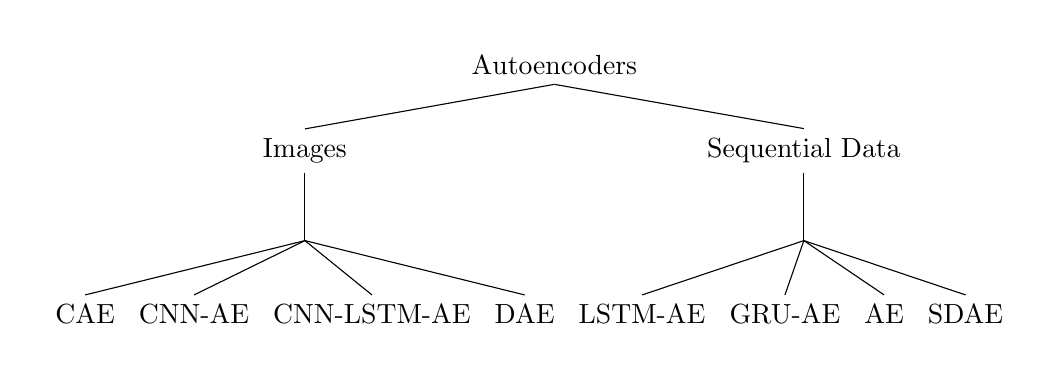
\begin{tikzpicture}
\matrix
{
% \node{\Tree
%     [A.  \edge[blank];
%     [B.  \edge[blank];
%     [C. \edge[blank];
%     [D. ]]]]};
&
\node{\Tree
 [.Autoencoders
    [.Images
        [{CAE} {CNN-AE}  {CNN-LSTM-AE} {DAE} ] ]
    [.{Sequential Data}
            [ {LSTM-AE} GRU-AE AE SDAE ]]]};\\
};
\end{tikzpicture}
\caption{\textbf{Autoencoder architectures for anomaly detection}.
        \\AE: Autoencoders~\cite{liou2014autoencoder}, LSTM : Long Short Term Memory Networks~\cite{hochreiter1997long}
        \\SDAE: Stacked Denoising Autoencoder~\cite{vincent2010stacked}, DAE : Denoising Autoencoders~\cite{vincent2010stacked}
        \\GRU: Gated Recurrent Unit~\cite{cho2014learning}, CNN: Convolutional Neural Networks~\cite{krizhevsky2012imagenet}
        \\CNN-LSTM-AE: Convolution Long Short Term Memory Autoencoders~\cite{haque2018image}
        \\CAE: Convolutional Autoencoders~\cite{masci2011stacked}
        }

 \label{fig:aevariants}
\end{figure}
Autoencoders are simple and effective architectures for outlier detection. However, the performance gets degraded  due to noisy training data with a large fraction of corruptions~\cite{zhou2017anomaly}.


%!TEX root = ../main.tex
\section{ Relative Strengths and Weakness : Deep Anomaly Detection Methods}
\label{sec:relativeSOW}
Each of the deep anomaly detection (DAD) techniques discussed in previous
sections have their unique strengths and weaknesses. It is critical to understand which
anomaly detection technique is best suited for a given anomaly detection problem.
Given the fact that DAD is an active research area, it is not feasible to provide such an
understanding for every anomaly detection problem. In this section we analyze the
relative strengths and weakenesses of different categories of techniques for a few
simple problem settings.\\
Classification based supervised  or semi-supervised techniques illustrated in Sections ~\ref{sec:supervisedDAD, sec:semi_supervised_DAD} are  better choices in scenario consisting of equal amount of labels for both normal and anomalous instances. The computational complexity of an DAD technique is a key aspect, especially when the technique is applied to a real domain. While classification
based, supervised or semi-supervised techniques have expensive training times, testing is usually fast. Unsupervised DAD techniques presented in Section~\ref{sec:unsupervisedDAD} are being frequently applied since
label acquisition is very expensive and time consuming process. Most of the unsupervised deep anomaly detection requires priors to be assumed on the anomaly distribution and models are less robust in handling noisy data. Hybrid models illustrated in Section~\ref{sec:hybridModels} extract robust features within hidden layers of deep neural network, and feed to best performing classical anomaly detection algorithms. The hybrid model approach is suboptimal because it is unable to influence representational learning in the hidden layers.  The One class Neural Networks  (OC-NN) described in Section~\ref{sec:oneclassNN} combines the ability of deep networks to extract progressively rich representation of data alongwith the one-class objective, such as an hyperplane~\cite{chalapathy2018anomaly} or hypersphere ~\cite{ruff2018deep} to separate all the normal data points from the origin.





%!TEX root = ../main.tex
\section{Conclusion}
\label{sec:conclusion}
In this survey we have discussed various research methods in deep learning-based anomaly detection
alongwith its application across various domains. This article discusses the challenges in deep anomaly detection and presents  several existing solutions to these challenges. For each category of deep anomaly detection techniques, we present the assumption regarding the notion of normal and anomalous data.  The goal of this survey was to investigate and identify the various deep learning models utilized and its suitability for a given dataset. When choosing a deep learning model to a particular domain or data, these assumptions can be used as guidelines to assess the effectiveness of the technique in that domain. Deep learning based anomaly detection is still an active research, a possible future work would be to extend and update as more mature techniques are proposed.




% \section{ General Framework for Group Deviation Detection
}
 \label{Sec:Framework}
In the last section, we clearly defined the problem of detecting group deviations in static and dynamic situations.   
  This section elaborates  upon the general framework and underlying structure for GAD and GCD techniques. Discovering significant group deviations is related to three sub-problems. 
\begin{enumerate}[1.]
\item {\it Group Structures}:  The definition of groups and the relationship between data instances is important to understand. %  clustering algorithm aggregate data instances into group structures.
\item {\it Statistical Properties}:  
A variety of statistical properties may characterise group deviations. % For example, a user is able to examine statistical properties of interest such as proportions, location or dependence.
 If statistical properties  are  not adequately quantified then relevant group deviations cannot be identified.
\item  {\it Model Design}: 
 The design of GAD and GCD techniques include data inputs,   model assumptions, learning approaches and output information. 
\end{enumerate}


\subsection{Group Structures}
We now highlight examples of different problems associated with group structures.   A group is a collection of two or more related data instances where Tan et al.  \cite{Tan} state that a data instance is synonymous with terms such as  vector, sample, entity, observation, etc. %Many GAD techniques assume that features from members in a group are independent and identically distributed (iid) where
Members in a group can be related by  external information of known group labels such as in topic modelling where Xiong et al. \cite{FGM} consider a document as a group of  words or a corpus as a group of documents. When group structures are not previously known, clustering algorithm aggregate data instances based on similarity criterion. 
 For example, Xiong et al. \cite{MGM} infer a spatial cluster of galaxies with distances closer than 1 megaparsecs while Wong et al. \cite{wong-rule} examine a demographic group of patients  based on certain categorical features.  
%   The interpretation of results relies on initial definition and construction of group structures. 
  
When group structures are unknown a priori,  clustering algorithms are applied. Common procedures minimise the cumulative  distance  between  members in a group to a central reference point. %These algorithms such as $k$-means or  nearest neighbors
 Clustering algorithm  for numerical values  are discussed in Jain \cite{jain2010} where a group of data instances contains members with similar features based on minimising distance metrics.   
Steinbach \cite{steinbach2004} discusses issues with distance-based clustering algorithms as data points become difficult to differentiate in higher dimensions.   More sophisticated techniques have been specifically developed for group  
%In particular,
 group deviation detection   %techniques infer clusters based on different criterion 
 such as:
\begin{enumerate}[-]
\item Chen et al.  \cite{GLETS}  apply density-based spatial clustering based on Pearson's correlation and Euclidean distance between values of times series. 
%\item Chen et al.  \cite{Chen2014} examine Pearson's correlation and Euclidean distance between values of times series.  
\item    Yu et al. \cite{GLAD} examine individual features as well as pairwise connection data.  %infer groups containing a mixture of social roles for social media applications. 
\item Soleimani and   Miller \cite{ATD} infer anomalous clusters of documents based on likelihood probabilities.
\item Dai et al. \cite{ERACD} cluster based on the ranking of feature values. 
\end{enumerate}
Therefore there are many procedures for clustering data instances when group structures are previously unknown.


\begin{figure}[h]
\centering
   \begin{subfigure}{1\linewidth} \centering
     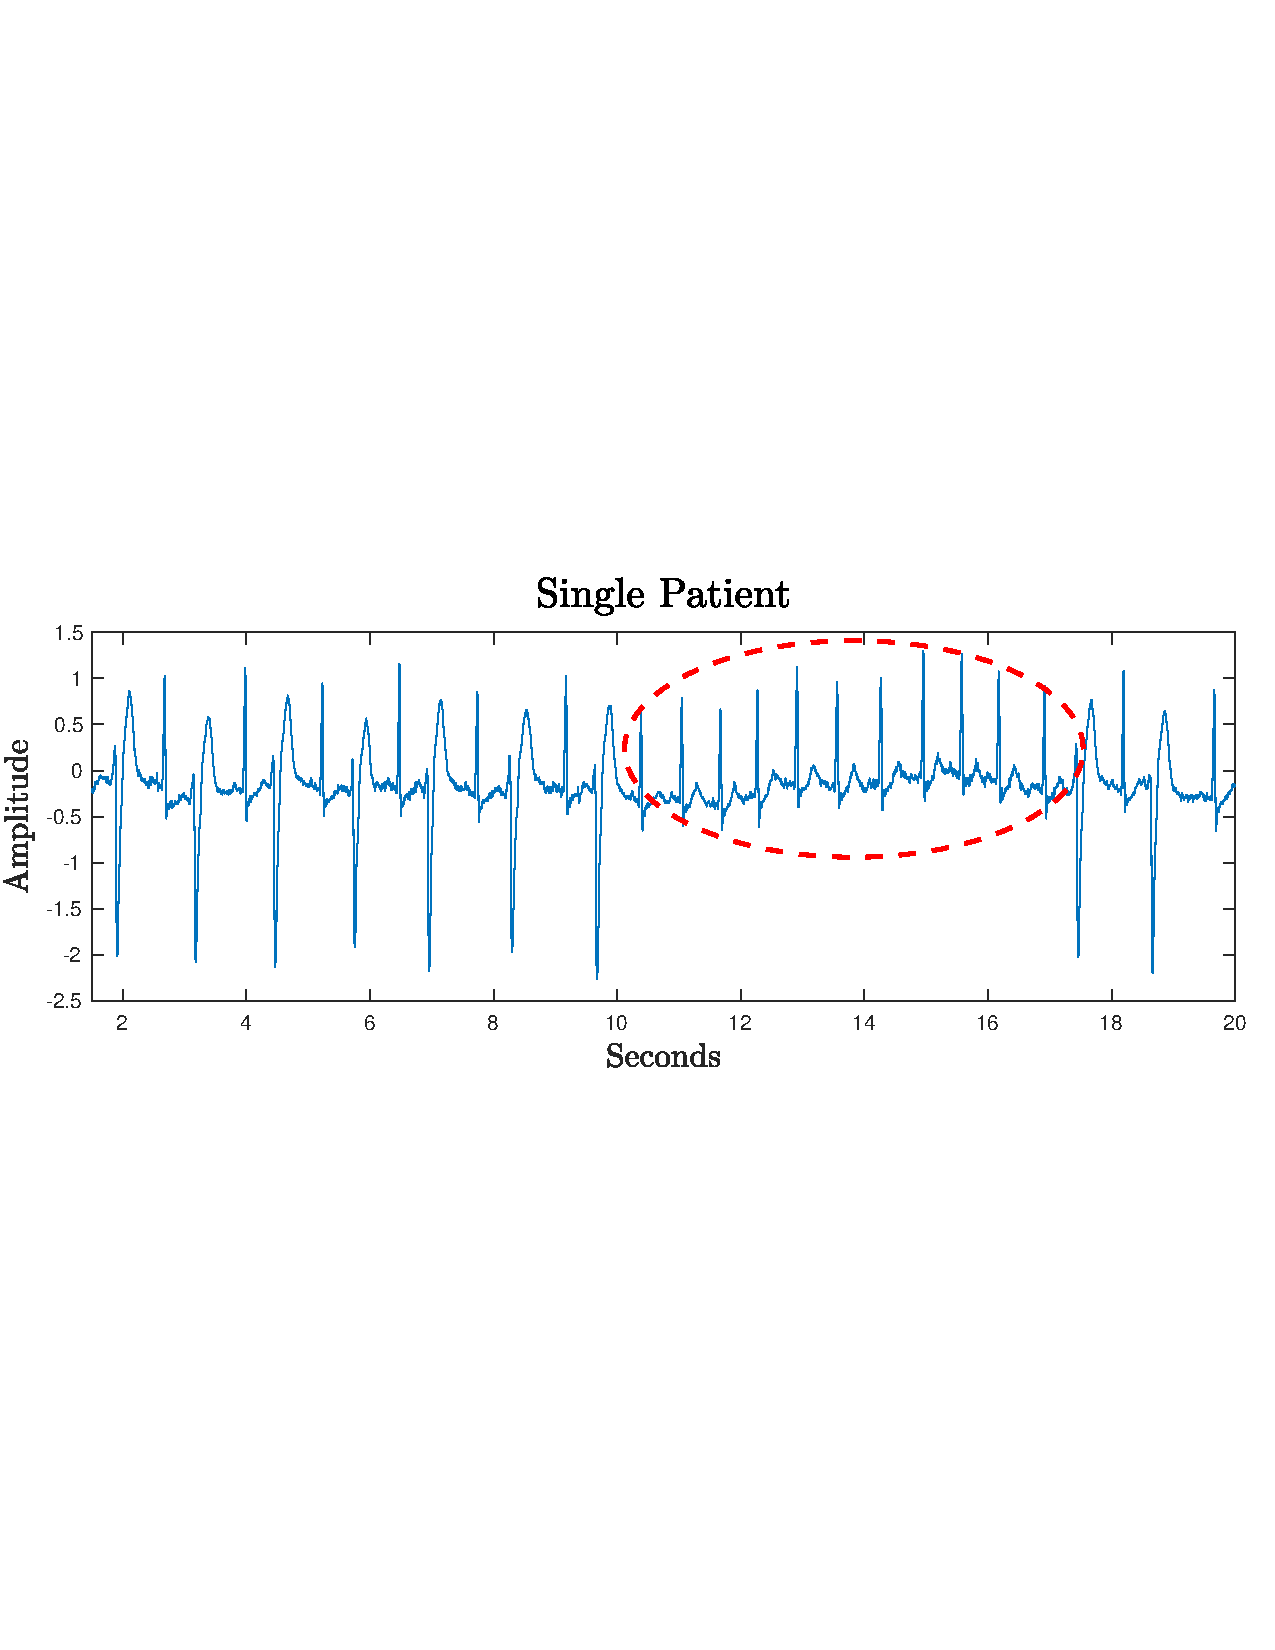
\includegraphics[width=6cm, height=4cm,trim=5cm 9.5cm 4.5cm 9cm]{FIGURES/ECGa}
     \caption{A collective anomaly (red dotted circle) in the ECG reading of a single patient.}
   \end{subfigure}
   \begin{subfigure}{1\linewidth} \centering
     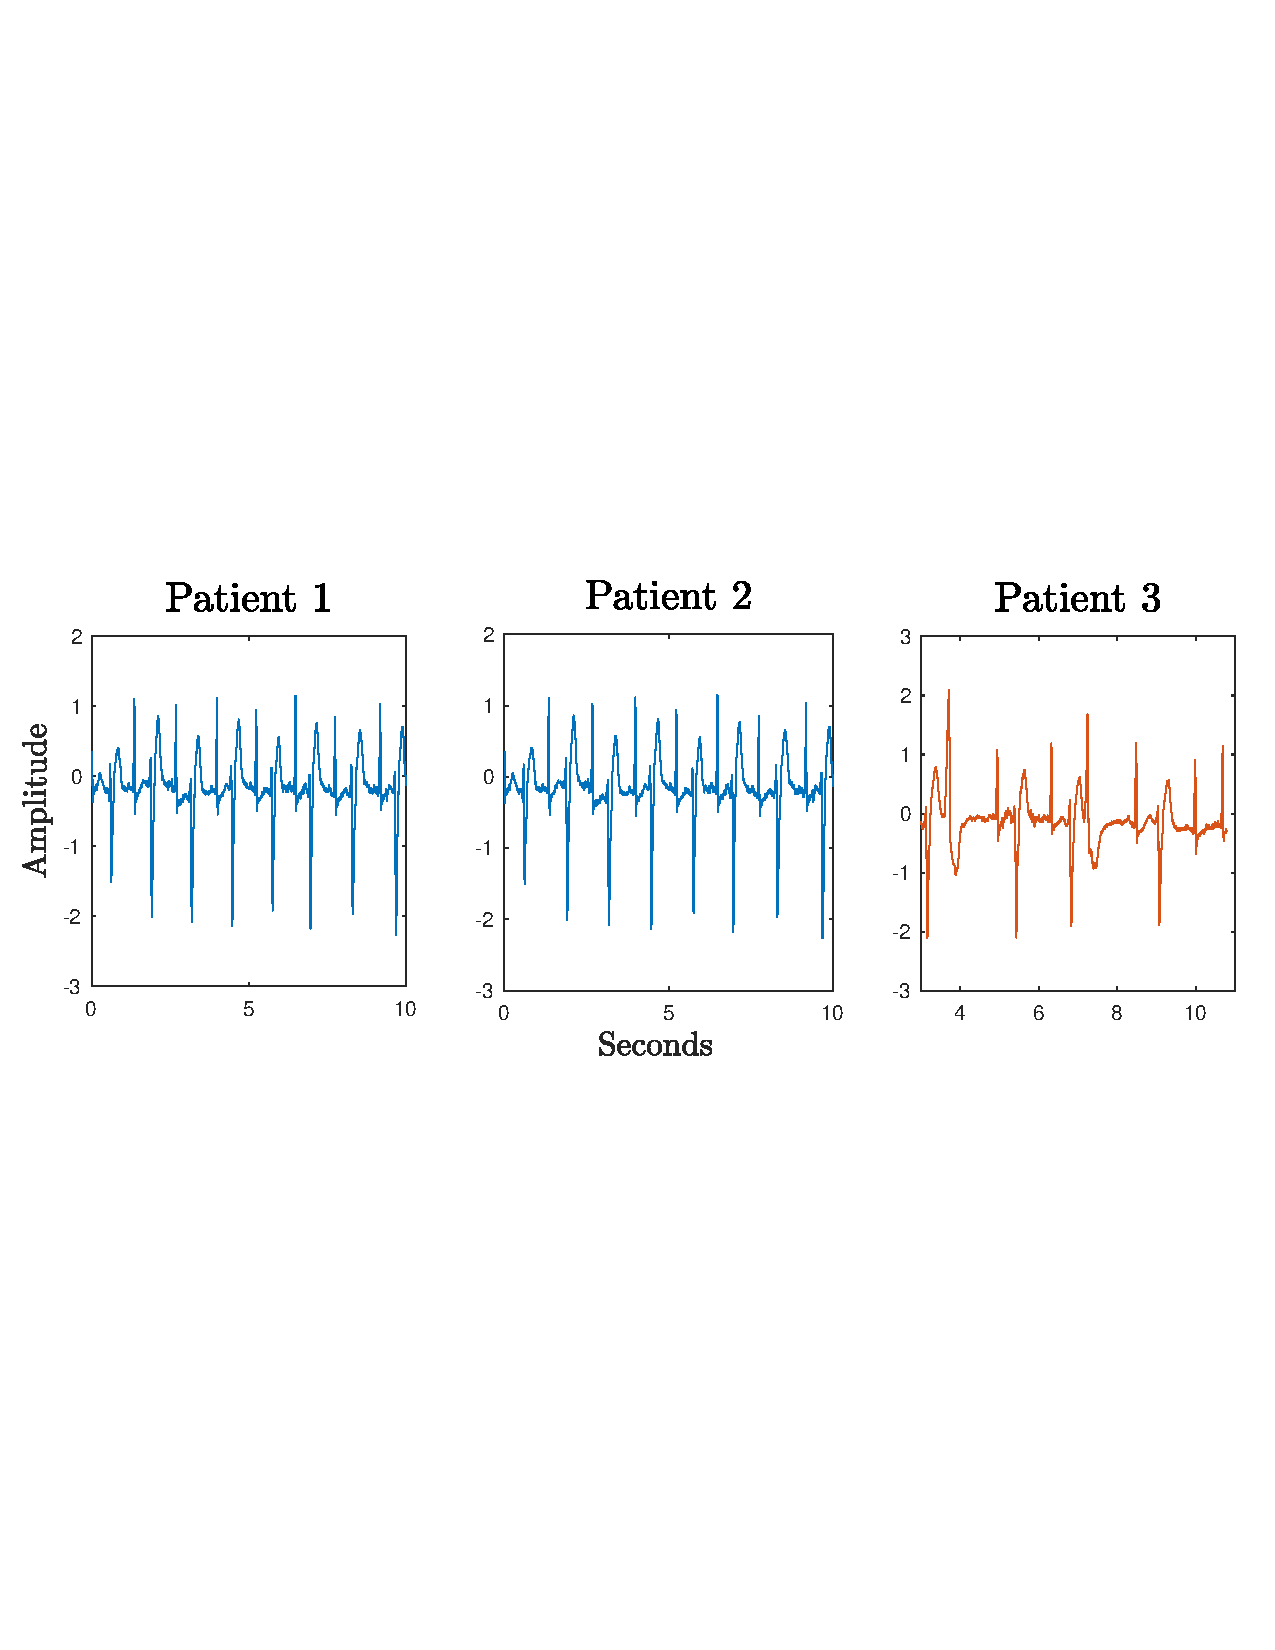
\includegraphics[width=6cm,  height=4cm,trim=5cm 9.5cm 4.5cm 8.5cm]{FIGURES/ECG}
     \caption{A group anomaly (Patient 3) is observed when comparing several patients.} 
   \end{subfigure}
  % \vspace{-1cm}
\caption{ In (a), a collective anomaly is a collection of related data instances that is anomalous with respect to time-dependent observations from  a single patient.   
In (b), a group anomaly is a specific example of a collective anomaly where  the entire dataset involves a group of observations from multiple patients. 
 } \label{Fig:ECG}
\end{figure}
%\vspace{1cm}


 
 
In our thesis, we do not use group anomaly and  collective anomaly interchangeably.  Chandola \cite{Chandola} defines a collective anomaly  as "a collection of related data instances that is anomalous with respect to the entire dataset." 
A group anomaly is specific example of a collective anomaly where  
the entire dataset involves multiple groups. % in the dataset. 
To differentiate these terms, consider the electrocardiogram (ECG) example from Goldberger et al. \cite{Goldberger}.  Figure \ref{Fig:ECG} (a) highlights a collective anomaly (in the dotted red circle) that exhibits an irregular pattern as compared to the  entire dataset (time series of a single patient). For a GAD application,  Figure \ref{Fig:ECG} (b) illustrates ECG readings from several patients  where  Patient 3 represents a group anomaly as the statistical properties are significantly different.  %however this is also a collective anomaly as the entire dataset can be considered as information from all of the patients.
 A realistic GCD case  would involve a group of patients with ECG readings similar to Figure \ref{Fig:ECG} (a) where a large-scale phenomena affects all patients around $\tau=10$. 
 


\subsection{Statistical Properties}
% SP - known vs unknown
 In some cases, a domain expert is interested in particular  statistical properties of groups. Statistical properties are measured and compared for group deviation detection. In terms of point-based and distributed-based group behaviours, point-based group deviations are characterised by a central location while distributed-based group deviations are characterised by statistical properties other than location such as scale, shape or dependence. In practice, group deviations are difficult to detect as a combination of statistical properties may  significantly differ. If a user is able to specify statistical properties of interest, group deviations are more easily detected and interpreted. 

 Since there are also many ways to quantify statistical properties of groups, we describe common parametric and non-parametric measures for statistical properties in Table \ref{Tab:Des} where non-parametric measurements are more robust to individual outliers. %Statistical properties in Table \ref{Tab:Des}, capture group  behaviours  for continuous variables however other metrics are more suitable for discrete or categorical datasets. 
   Given prior knowledge of statistical properties that characterise group deviations for GAD or GCD applications, a suitable method for discriminating groups is easily constructed. However when the nature of significant group deviations in terms of statistical properties is unknown, more   specialised techniques are required.  
 
 
		\begin{table}[h]
%\renewcommand{\arraystretch}{1}
	\tabcolsep=0.1cm
	\begin{center}
   \scalebox{0.88}{
	\begin{tabular}{lccc  }
	\hline\\[-2mm]
		%\multirow{ 2}{*}{} & & & \\[2mm]
 Statistical & %Function &
	 Parametric Measures% in $\boldsymbol \alpha$ 
	 &  Non-parametric Measures %  in  $\boldsymbol \gamma$ 
	 \\[-1mm]  Property & & &
	 \\[2mm] \hline\\[-2mm]
		\multirow{ 2}{*}{Location } & %	\multirow{ 2}{*}{$h_1$ }&
	  $ \displaystyle\bar{ {X}}_v=\frac{1}{N} \sum_{n=1}^N X_{nv}$ & $  \displaystyle \hat{q}_v({0.5})$  \\
	 & \hspace{5mm}(mean) & (median)  \\%[2mm]
	  %
	\multirow{ 2}{*}{Scale} & %\multirow{ 2}{*}{$h_2$} &
	 $ \hat\sigma^2_v = \displaystyle	\frac{1}{N-1}\sum_{n=1}^{N} \big(X_{nv}-\bar {X}_v \big)^2$  &  % \displaystyle s^2 =	\(\stackunder[1pt]{$ \mbox{mediai}$}{	\scalebox{0.8}{$ 1\le i\le N$}} \) $\big (| X_n - q_{0.5}| \big)$ 
	$\displaystyle \hat{q}_v({0.75}) - \hat{q}_v({0.25})$ \\ %[-1mm]
	 & (variance) &(interquartile range)   \\[1mm]
	 Skewness & % $h_3$ &
	$\displaystyle\frac{1}{N} \sum_{n=1}^N \frac{( X_{nv}-\bar{X}_v)^3}{ \hat\sigma_v^3}  $  & 
	$ \displaystyle \frac{\hat{q}_v({0.9}) + \hat{q}_v({0.1}) -2 \hat{q}_v({0.5}) }{  \hat{q}_v({0.9}) - \hat{q}_v({0.1})  }$\\[4mm] %\displaystyle  \hat{\mathcal{S}}=
	 Kurtosis &  %$h_4$ &
	 $\displaystyle\frac{1}{N} \sum_{n=1}^N \frac{( X_{nv}-\bar{X}_v)^4}{ \hat\sigma_v^4}  $ &
	$ \displaystyle\frac{\hat{q}_v({0.975}) -\hat{q}_v({0.025}) }{\hat{q}_v({0.75}) -\hat{q}_v({0.25}) }  $ \\[4mm] %\displaystyle \hat{\kappa} =
	 	\multirow{ 2}{*}{Dependence} &  	%\multirow{ 2}{*}{$H$} &
	  $ \; %\hat \rho =
	   \displaystyle\frac{ \sum_{n} \big(X_{n1}- \bar X_{1} \big) \big(X_{n2} - \bar X_{2}\big) } {\sqrt{ \sum_n \big(X_{n1}- \bar X_{1} \big) ^2 \sum_n \big(X_{n2} - \bar X_{2}\big)^2 }   } $ & 
	\;\; $\displaystyle   \frac{ \sum_{n} \big(R_{n1} - \bar R_{1} \big) \big(R_{n2} - \bar R_{2}\big) } { \sqrt{ \sum_n \big(R_{n1} - \bar R_{1} \big) ^2 \sum_n \big(R_{n2} - \bar R_{2}\big)^2  }} $ \\
	 & (Pearson's correlation ) & (Spearman's rank correlation \cite{Spearman})\\[1mm] % \hat{\rho} = 
	 \hline\\[-2mm]
	 \end{tabular}
	 }
	\end{center}
	\caption{ Given a group ${\bf G} =(X_{nv})  \in \mathbb{R}^{ N \times V}$,  the $\beta$-quantile  $\hat{q}_v(\beta)$ is estimated from  the empirical distribution of the $v$th column of random variables. Also
$R_{\cdot v}  \in \mathbb{R}^{ N }$  denotes ranked values  of $X_{\cdot v}$ with average column rank $\bar R_v$.  % Note Pearson's correlation captures a linear relationship between variables whereas Spearman's rank correlation \cite{Spearman}  measures a monotonic (possibly non-linear) dependence.
Non-parametric measures of skewness and kurtosis are respectively described in 
Hinkley   \cite{hinkley1975} 
and Moors \cite{RobustK}.
}
 \label{Tab:Des}
\end{table}  
 
% SP - characterise, measure 
In most applications, statistical properties that characterises group deviations are usually known. Without prior information, it is difficult to differentiate a group deviation  as there may be a significant difference in a combination of statistical properties. %Also if an incorrect selection of statistical properties are analysed then significant group deviations cannot be identified. 
  Guevara et al. \cite{SMDD} explore the GAD application and find that more complicated group behaviours are not adequately characterised by single quantities such as location estimates of group distributions. %Their study investigates examples of Gaussian mixtures where a group anomaly is generated from a different proportion of distributions.
 % Another issue occurs for high dimensional datasets as common measures of statistical properties in Table \ref{Tab:Des} may not properly characterise the behaviour of groups.
   Topic models are applied for GAD problems  where  statistical properties of  groups represent  proportions of inferred topic  variables.  % high number of dimensions where  models extract . 
  We  discuss topic models in more detail for  GAD applications in Chapter \ref{sec:staticGAD}.   



\subsection{Model Design} 
After understanding problems associated with group structures and statistical properties of interest, a domain expert can construct suitable solutions for GAD and GCD problems. Firstly models are designed to be compatible for specific types of input data such as continuous or categorical variables. To appropriately identify group deviations, discriminative methods do not impose data assumptions  while generative models assume how data is generated.  Given availability of labeled group behaviours, models either apply  supervised or unsupervised learning. Another important aspect of model design is  interpreting outputs with scores or labels.  The model design of group deviation detection techniques requires a clear understanding. 

\subsubsection{Input Data }
Certain models are compatible for specific types of input data.   As specified by Equation (\ref{Eqn:Domain}) in the problem definition, data types that are explored in GAD and GCD applications include  discrete, continuous or categorical features.
Data types also influence the appropriateness of statistical properties for characterising  groups behaviours. In particular, generative models are flexible in assuming a Gaussian distribution for continuous real-valued data whereas categorical features are modelled by categorical distributions.   
 Pairwise network connections are also a possible type of input data and are usually  incorporated for clustering when group structures are previously unknown.  Similarly, certain clustering algorithms are only compatible for specific data types. 


 
\subsubsection{Assumptions}
 The assumptions of GAD and GCD techniques  are  discussed in terms of discriminative and generative models.  %where supervised or   unsupervised learning is applied depending on the availability of labeled data.  
Discriminative approaches are useful for directly classifying groups into regular and anomalous behaviours without knowledge of how data is generated.  %Due to the lack of regular and anomalous group labels, discriminative GAD techniques classify regular behaviour based on the predominant group pattern.  
 On the other hand, generative models assume specific probability density functions over   variables.  Hypothesis tests are a special type of generative model that further classify group deviations. %GAD and GCD  techniques  are classified as either  discriminative or generative models however hypothesis tests are also elaborated on.  
% Common advantages and disadvantages of 
Table \ref{Tab:DG} lists common advantages of  discriminative methods, generative models as well as hypothesis tests. % for  GAD and GCD  applications. 

\begin{table}[H]
	\tabcolsep=0.3cm
	\renewcommand{\arraystretch}{1.2}
	\begin{center}\scalebox{1}{
	\begin{tabular}{lcccccccccccccccc  }
	\hline\\[-6mm]
 Procedure & $\mathcal{A}1$ & $\mathcal{A}2$ & $\mathcal{A}3$ & $\mathcal{A}4$ & $\mathcal{A}5$  \\[-1mm] \hline \\[-8mm] \hline\\[-6mm]
  Discriminative Methods   & \yeah & \nope & \yeah  & \nope & \nope \\
  Generative Models   & \nope & \yeah & \nope  & \yeah & \nope \\
 Hypothesis Tests  & \yeah & \yeah & \nope  & \yeah & \yeah\\[3mm]
\hline 
	 \end{tabular}
	}
	\end{center}
	\medskip
		\caption{  Summary of advantages of   group deviation detection techniques in terms of 	 discriminative methods, generative models and hypothesis tests. If a procedure has a particular advantage, a tick label is present whereas if a procedure lacks an advantage, a cross is displayed.  }
	%\vspace{-5mm}
 \label{Tab:DG}
\end{table}  

	
	
\begin{enumerate}[{$\mathcal{A}$}1] \setlength\itemsep{5pt}
\item   {\it Direct classification}:  discriminative models and hypothesis tests provide explicit boundaries between regular   behaviours and significant group deviations. 
 \item  {\it Rich Interpretation}: Results from discriminative methods  are difficult to interpret due to the complex representation between group   variables. For explanatory purposes, 
  generative models offer a rich interpretation of  groups and inferred statistical properties.    The flexible structure of generative models is also useful for incorporating prior information.
  \item  {\it  Minimal  Assumptions}: 
  Discriminative approaches assume that group behaviours can be differentiated based on certain optimisation criteria.   Generative models further impose distributional assumptions which are not  appropriate for all datasets. 
  \item  {\it Prevents Overfitting}: Discriminative methods are prone to overfitting model parameters especially on  training data with smaller sample sizes. 
 Generally, generative models experience less overfitting  when the model assumptions are appropriate for given datasets.  
   \item  {\it Statistical Significance}: In addition,  hypothesis tests determine whether the statistical properties of a group is significantly different. In many cases, generative models arbitrarily classify    significant group deviations based on highest anomalous scores. 
\end{enumerate}	




\subsubsection{Learning}
Supervised learning requires previously labelled group behaviours while  
unsupervised approaches learn the dominant pattern in the dataset. 
When surveying current state-of-the-art group deviation detection 
 techniques, most discriminative  and generative models employ unsupervised learning.  
 Unsupervised learning is preferred as  ground truth labels of regular or irregular behaviours are not usually available. In a  comparison study conducted by Laskov et al. \cite{laskov2005learning},  unsupervised methods achieve a higher accuracy than  supervised algorithms when learned behaviours from a training data do not account for unknown patterns in a test set.  Unsupervised methods are beneficial for  discovering novel group patterns. 

\subsubsection{Output}
The output from group deviation detection techniques  is given by classification labels or  scores indicating significant group deviations.  
 Discriminative methods produce binary labels for regular or anomalous classes in GAD while GCD methods estimate times of significant change in a dynamic group over time.   Generative models  tend to compute scores that quantifies the degree that a  group is significantly different as compared to other groups in a dataset. Scores from generative models are often converted to a classification by a threshold chosen by a user however  this selection is subjective and equivocal.  Hypothesis tests are advantageous for obtaining classification labels based on the statistical significance of group deviations.  
  

  




\section{Challenges}
We now discuss challenges associated with group deviation detection. There are many issues that arise from inadequate group definitions in a dataset. Datasets involving group structures are more difficult to understand and analyse than many pointwise data problems with potential absence of group labels. Benchmark datasets are currently unavailable and thus comparison studies are difficult to conduct. Even though detecting group deviations may seem like a straightforward task, results require validation and careful interpretation. The challenges in  GAD and GCD applications  include:

\begin{enumerate}[\textbullet]
\item {\it  Defining Groups}:
 F\~{a}rber et al. \cite{ClusterEval}   highlight that known group labels may not represent natural clustering patterns in a dataset. 
 However when group memberships are unknown a priori,   clustering method possibly lead to inadequate group representations. Group structures  may be improved by incorporating additional information such as known regular group behaviour or pairwise relationships between data instances. 
 \item {\it Defining Group Deviations}: Group deviations can be defined based on the number of groups or the number of  data instances within groups. Usually when groups possess similar sizes, group deviations occur as a minority of group observations.    
  % Consider  a single group that contains more observations than the total number of other groups. 
\item {\it Capturing Statistical Properties}: Group deviations may occur in a variety of statistical properties such as location, scale, shape, etc.    Borgatti et al. \cite{GroupSocialMedia} explain that more complicated patterns exist when each member contributes to behaviour of a group. Thus an effective detection method has to adequately capture properties of groups in order to identify significant deviations.
% \item {\it Evolving Patterns}: In many domains, the notion and definition of group deviations also changes over a period of time. Algorithms that can adapt to identifying evolving unknown group patterns  are preferable in many applications. 
\item {\it Not statistically significant}: Many methods classify or score group behaviours however they do not quantify statistical significance. In many cases, it is difficult to distinguish noisy group observations from a significant group deviation. 
\item {\it Absence of Group Labels}: When group memberships are unknown a priori, clustering  induces additional uncertainty in analysis and subsequent results. Halkidi et al. \cite{ClusterValidity} explain that it is also difficult to evaluate the effectiveness of inferred clusters without sufficient ground truth labels. 
\item {\it Absence of Ground Truth Labels}: Like other anomaly detection applications, ground truth labels are usually unavailable. To investigate group deviations rather than a single  instance, requires more time and effort for obtaining  ground truth labels.  
\item {\it Absence of Benchmark Datasets}: Since there is a lack of benchmark group datasets, many methods resort to anomaly injection. Anomaly injection involves contaminating a real-world dataset with significant deviations and subsequently comparing detected instances with  ground truth labels. This does not account for  anomalies that are naturally present in a dataset such that injected anomalies should possess higher deviations than naturally occurring anomalies. 
\item {\it Absence of Robust Comparison Studies}: Evaluative metrics that assess  group deviation detection datasets would be useful for a robust comparison study. For pointwise anomaly detection methods, Campos et al. \cite{Campos2016} propose two measures for a dataset; difficulty of detecting different types of anomalies and diversity or agreement between scores computed from methods.  A similar evaluative process is recommended for group deviation datasets to provide a more robust comparison of state-of-the-art techniques. 
\end{enumerate}
There is no single solution that overcomes all of these challenges in GAD and GCD research.  We further elaborate on related work for group deviation detection techniques in static and dynamic scenarios. 


\section{Related Work}
Due to continual research involving  anomaly detection and change detection,  there are additional problems and  techniques that are proposed after the publication of many papers. Extensive reviews on pointwise anomaly detection techniques are conducted by Hodge and  Austin \cite{Hodge}  as well as Chandola et al. \cite{Chandola}.   Since change detection is a general topic, many techniques are domain specific where  
Singh \cite{singh1989review} examines the application to remote sensor data while Reeves et al. \cite{reeves2007review} explore change detection techniques for climate data. An overview of temporal outlier detection is provided by Gupta et al. \cite{Gupta2013}. Many of these papers  briefly discuss  group applications however GAD and GCD are emerging areas of research where most state-of-the-art techniques have been more recently developed.  Yu et al. \cite{SurveySocialMedia} and  Xiong \cite{Collective}  provide descriptions of current state-of-the-art GAD methods.  % 

{  
GAD is closely related to zero-shot learning (ZSL) where data instances are classified however their behaviour may not be seen in training. % different classes even when unseen instances in a test set   that are not present in the training set.
%There is an overlap between GAD and zero-shot learning (ZSL) techniques however there are fundamental difference. 
Surveys on ZSL have been conducted by Xian et al. \cite{ZSLsurvey} where ZSL assumes a subset of classes (groups) are known during training whereas GAD techniques are more general as none of regular  group behaviours (classes) may be available.
%GAD is more general than ZSL as classes (groups) may not be available while ZSL assume classes are known during training.     
 %ZSL accounts for the simple case where training and test set are disjoint while classes in  training and test set may overlap for generalised ZSL. 
  Without known classes,  Kodirov et al. \cite{unsupervisedZSL} propose an unsupervised ZSL technique that incorporates auxiliary textual information.   ZSL techniques are specfically formulated for certain domains such as image classification \cite{ZSLanomaly} and network intrusion  \cite{perez2016} however we focus on GAD techniques that are applicable for more general domains. 



%Group change detection  
Similarly the GCD problem has been  specifically formulated for many real-world applications. In video change detection, a video can be modelled as a group of color pixels or visual features where  significant deviations in video frames are detected over time. Lienhart 
\cite{VideoSurvey} provides a survey of video transition (gradual change) detection techniques while a comparison study of performance for video-shot-change (abrupt  change) detection algorithms is conducted in Gargi et al. \cite{gargi2000}. %Other methods such as  Yuan et al. \cite{yuan2017anomaly} identify subtle changes in  traffic scenes while  %Yuan et  al.   \cite{yuan2016hyperspectral} examine  reflectance spectrum data.
%Rout et al. \cite{rout2018}  detect changing  positions of dynamic objects in an underwater video.
  In other applications, Sakaki et al. \cite{sakaki2010} detect an earthquake event by monitoring a group of keywords on Twitter and  Xie et al. \cite{xie2013} explore  sequential change-point detection in multiple sensor readings over time. % the average value of  sensor readings over time. % and also estimate the affected proportion  of sensors at a specific time step.  
Many of these GCD techniques are only applicable in  specific domains and are not flexible for detecting changes in a variety of statistical properties.   
}


% \section{Conclusion
 } \label{Sec:Conclusion}
 This paper has used the contemporary bidirectional LSTM-CRF, for clinical concept extraction. The most appealing feature of this sytem   is their ability to provide end-to-end recognition initialized with general purpose off-the-shelf word embeddings sparing effort from laborious feature construction. To the best of our knowledge, ours is the first paper to adopt bidirectional LSTM-CRF for concept extraction from clinical records. The experimental results over the  2010 i2b2/VA reference standard corpora look promising, with the bidirectional LSTM-CRF ranking closely to the state of the art. A potential way to further improve its performance would be to initialize its training with unsupervised word embeddings such as Word2Vec~\cite{Mikolov:13} and GloVe~\cite{Pennington:14} trained with domain specific resources such as Monitoring in Intensive Care (MIMIC) II copora. This approach has proved effective in many other domains and still dispenses with expert annotation effort; we plan this exploration for the near future.








% % GAD Survey
% \chapter{Group Anomaly Detection (GAD) }  
 \label{sec:staticGAD}
%\section{ Group Anomaly Detection (GAD) Techniques} \label{Sec:GAD}
% Brief paragraph 
After setting up the group deviation detection  problem and describing the general framework for methods in previous sections, we now  explain specific GAD techniques in further detail. 
 GAD involves comparing multiple groups and identifying groups with significantly different statistical properties.  Following the problem definition in Section   \ref{Sec:Problem}, 
${\bf G}_m= \Big ( {X}_{mnv}\Big) \in \mathbb{A}^{N_m \times V}    $ 
where domain $\mathbb{A}$ depends on the   input data type such as  categories, discrete value or continuous variables.
 GAD methods are explained by descriptive key components from Section   \ref{Sec:Problem} in  categories of discriminative methods,  generative models and hypothesis tests. 

% A description of GAD techniques is provided 


\section{ Discriminative Methods } 
 In GAD, a discriminative method classifies input groups into regular and anomalous behaviours.     
We  elaborately discuss two state-of-the-art discriminative models for detecting group anomalies.  Firstly One-Class Support Measure Machine (OCSMM)   proposed by Muandet and Sch\"olkopf \cite{OCSMM} %supports unsupervised learning for classifying group behaviours,  OCSMM 
is an unsupervised method that maximises the margins between two classes using a separating hyperplane.  
 Another discriminative model Support Measure Data Description (SMDD)   proposed by Guevara et al. \cite{SMDD} is similar to OCSMM however uses a supervised approach  based on a minimising the  volume sets that contains the majority of groups in a training set.  % are contained in boundaries (soft or hard) of a volume set. 
  Both methods can handle continuous and discrete input data where it is assumed that the statistical properties of group deviations can be differentiated based on certain  optimisation criteria. 
  
 In this analysis, each  group   is associated with a probability measure where observations  are assumed to be  independent and identically distributed (iid). 
Formally, %on the  space $(\Omega,\mathcal{F})$
given an  outcome space $\Omega$ and $\sigma$-algebra $\mathcal{F}$, we define a set of probability measures $\mathcal{P}=\{\mathbb{P}_1,\dots,\mathbb{P}_M\}$  
where each function is given by $\mathbb{P}_m: \, \Omega \to [0,1]
$ for $m=1,\dots, M$. 
  % The set of all probability measures  $\mathcal{P}_\Omega$  is defined on the probability space $(\Omega,\mathcal{F},\mathbb{P})$. 
If groups  ${\bf G}_1,{\bf G}_2,\dots,{\bf G}_M$ exhibit regular behaviour then they have iid probability distributions specified by $\mathbb{P}_1,\dots,\mathbb{P}_M$.   
 In both OCSMM and SMDD, mean embedding functions are applied to transform groups into points in a reproducing kernel Hilbert space (RKHS). 
   Let $\mathcal{H}$ denote the RKHS of probability measures with   kernel $k:\Omega \times \Omega  \to\mathbb{R}$.  Group behaviours are characterised using mean kernel embedding functions as defined by 
 \begin{align}
\mu :  \mathcal{P}\to \mathcal{H}, \quad\mathbb{P}_m \mapsto \mu_{\mathbb{P}_m}=E_{\mathbb{P}_m} [ k({\bf G}_m,\cdot) ] =\int_{\Omega} k(u,\cdot)\, d\mathbb{P}_m(u).  \label{KMF}
 \end{align}
 for $m=1,\dots,M$. 
 

  

\subsection{ One-Class Support Measure Machine (OCSMM) }
 Muandet et al. \cite{OCSMM} propose OCSMM for  discriminating between regular and anomalous  group behaviours using a parametrised hyperplane. OCSMM maximises
 the margin between two classes as separated based on the hyperplane.  
{  Since OCSMM is  analogous to one class support vector machines  \cite{OCSVM}, we describe a linear hyperplane for vector ${\bf x}$ as } 
\[ %f_{\bf w}(x) = 
\big\langle {\bf w}, {\bf x} \big \rangle = \rho \]
where parameters $({\bf w}, \rho)$ are the weights and bias term for parametrising a separating hyperplane respectively.  Regular behaviours are further away from  the origin than anomalous instances. 

OCSMM allows the user to select the expected proportion of group anomalies in the training data as denoted by  $\nu \in (0,1)$.  Since group anomalies are assumed to occur much less frequently that regular groups,  OCSMM learns patterns from one-class that exhibits  the dominant behaviour in a dataset.  
For more flexible margins in a separating hyperplane, 
slack variables $\xi_1,\dots,\xi_M$ are  introduced such that the parameters  of a separating hyperplane are estimated by optimising the following problem %results in the optimisation problem 
%\vspace{-1cm}
 \begin{align}
&\min_{(  \rho, {\bf w},\boldsymbol \xi)} 
\frac{1}{2} \langle {\bf w},{\bf w} \rangle_{\small \mathcal{H}} - \rho +  \frac{1}{\nu M} \sum_{m=1}^M
\xi_m  \label{minW} \\
\mbox{with con}\mbox{straints: } &  \langle {\bf w} ,  \mu_{\mathbb{P}_m } \rangle_\mathcal{H} \ge \rho - \xi_m \mbox{ and } \xi_m \ge 0 \mbox{ for } m=1,\dots,M   \nonumber
\end{align}
%and the parameters ${\bf w},\,\rho$ and  $\boldsymbol\xi$ are
 The first term in Equation (\ref{minW}) represents  minimising the error or distance of separating data points from the origin. The slack variables offer a more flexible description of a separating hyperplane where penalty term $1/{\nu M}$ represents the trade-off between the distance of a hyperplane from the origin and the upper bound on expected number of group anomalies in a training set.  
Equation (\ref{minW}) can be solved by introducing Lagrange multipliers $\boldsymbol \alpha$ where the estimated hyperplane is %estimated by %with weights % $\bf w$ %simplified as 
\begin{align*}
 f_{\bf w}(\mu_{\mathbb{P}_m } ) = \big\langle {\bf w},\mu_{\mathbb{P}_m } \big \rangle_\mathcal{H} \quad %= \sum_{l} \alpha_l \, \langle \mu_{\mathbb{P}_m}, \mu_{\mathbb{P}_l}\rangle_\mathcal{H} \\
\mbox{ where }{\bf w}= \sum_{m=1}^M \alpha_m  \mu_{\mathbb{P}_m} \mbox{ and } \sum_{m=1}^M \alpha_m=1
%0 \le \alpha_m \le \lambda
\end{align*} 
 
The following schema describes OCSMM in four key components:   
 \begin{enumerate}[1.]
\item Characterisation function $f_1({\bf G}_{train})={\bf w}$: \\ The training set of group behaviours contains information about  $\mu_{\mathbb{P}_1},\dots, \mu_{\mathbb{P}_M}$.  In particular, the weight function of a separating hyperplane characterises a group training set by
\[{\bf w}= \sum_{m=1}^M \alpha_m  \mu_{\mathbb{P}_m}\] 
 \end{enumerate}
 %
 \begin{enumerate}[2.]
 \item Characterisation function $f_2({\bf G}_{test})=\mu_{\mathbb{P}_m}$: \\ 
The $m$th group is characterised by the mean embedding function $\mu_{\mathbb{P}_m}$.  Intuitively group observations are mapped onto the RKHS as group feature  representations. 
\end{enumerate}
 %
\begin{enumerate}[3.]
\item Measure $ \mathcal{D}\big( f_1({\bf G}_{train}), f_2({\bf G}_{test})\big )$ using a separating hyperplane: \\
The separating hyperplane compares characterisation functions ${\bf w}$ and $\mu_{\mathbb{P}_m }  $ with
$ \big\langle {\bf w},\mu_{\mathbb{P}_m } \big \rangle_\mathcal{H}%\sum_{l} \alpha_l \, \langle \mu_{\mathbb{P}_m}, \mu_{\mathbb{P}_l}\rangle_\mathcal{H}
$.   
 For a deeper understanding of this measure, consider  
\begin{align*}
 \big\langle {\bf w},\mu_{\mathbb{P}_m } \big \rangle_\mathcal{H}= \sum_{l} \alpha_l \, \langle \mu_{\mathbb{P}_m}, \mu_{\mathbb{P}_l}\rangle_\mathcal{H} 
\end{align*} 
where the kernel similarity on probability measures based on empirical samples is 
%To ensure the kernel similarity estimated on empirical samples   %K(\hat{\mathbb{P}}_m,\hat{\mathbb{P}}_l)=
\begin{align}
\langle \hat{\mu}_{\mathbb{P}_m},\hat{\mu}_{\mathbb{P}_l} \rangle_\mathcal{H}  
=
\frac{1}{N_m   N_l } \sum_{i=1}^{N_m}
 \sum_{i'=1}^{N_l} k\Big( X_{mi} , 
 X_{li'}  \Big)  \label{kernelest}
 \end{align}
%and $X_{mi}$ is the $i$th observation in the $m$th vector. 
%The following assumptions are imposed 
A reasonable approximation using empirical estimates for probability measures, requires   $||  \mu_{\mathbb{P}_m}  - \hat{\mu}_{ \mathbb{P}_m}  || $ is bounded   for $m=1,\dots,M$.   

  The selection of kernel similarity function $k$ is important in the detection of group anomalies.
When $k$ is chosen as a characteristic kernel such as a  Gaussian   kernel, the representative function $\mu$ is injective, that is there is a distinct mapping of groups onto the RKHS. The anomalous measure and classification threshold in  OCSMM are also dependent on the selection of kernel function. Table \ref{Tab:Kernel} provides examples where given a particular choice of reproducing kernel  $k$ in Equation (\ref{kernelest}), OCSMM characterises different statistical properties of  groups. 

 % of kernel functions that captures different statistical properties of groups. %For instance, a linear kernel only captures the behaviour of the first moment of a distribution while the  Gaussian RBF describes infinite moments.\\[2mm]

\end{enumerate}

 \begin{table}[H]
 
\begin{center}
\tabcolsep=0.25cm
 \scalebox{0.9}{
\begin{tabular}{p{15mm}ccp{20mm} } 
 \hline\\[-2mm]
Type & Reproducing Kernel $k(u,v)$  & Kernel Similarity $K(\mathbb{P}_m,\mathbb{P}_{l}  )$ & Moments  \\[1mm]
\hline \\[-4mm]
 \hline\\[-2mm]
Linear & $\langle  u,v \rangle $  & $0\, [Av \mbox{ if } \mathbb{P}=N(A,1)] $ & First\\[2mm]
Quadratic & $\langle  u,v \rangle ^2$   &  $v^2$ & Second \\[2mm]
Quadratic &  $(\langle  u,v \rangle +1)^2$ & $v^2+1$ & First \& Second \\[2mm]
Gaussian RBF & $\displaystyle \exp \bigg( {-\frac{||u-v||^2}{2\sigma^2} } \bigg)$ & $ \displaystyle \frac{1}{\sqrt{2}}\exp \bigg({-\frac{||v||^2}{4} } \bigg)  $ & Infinite
\\[-2mm]
& & $(\sigma^2=1)$ & 
 \\[1mm] \hline
\end{tabular}
}
\end{center}
%\vspace{-1cm}
 \caption{ Examples of different kernels for probability distribution $\mathbb{P}=N(0,1)$. % and the Gaussian RBF has a bandwidth or tuning parameter  $\sigma>0$.  
 }
 \label{Tab:Kernel}
\end{table}

 \begin{enumerate}[4.]
\item  Threshold $\epsilon= \rho$: \\  The  threshold term for OCSMM represents a bias parameter for the separating  hyperplane. This threshold is calculated from   groups with probability measures that are mapped closest to the separating hyperplane. In fact,   support measures provide a description for the separating hyperplane such that the $m'$th group with $ 0 <\alpha_{m'} < \displaystyle \frac{1}{\nu M}$ is a support measure  that satisfies 
\[ \rho  %=f_{\bf w}(\mu_{\mathbb{P}_m } )
 = \big\langle {\bf w},\mu_{\mathbb{P}_{m'} } \big \rangle_\mathcal{H}= \sum_{l} \alpha_l \, \langle \mu_{\mathbb{P}_{m'} }, \mu_{\mathbb{P}_l}\rangle_\mathcal{H}  \]
Then a threshold for anomalous groups is     \[\hat{\rho}=  \sum_{l} \hat{\alpha}_l \, \langle \hat{\mu}_{\mathbb{P}_{m'}}, \hat{\mu}_{\mathbb{P}_l}\rangle_\mathcal{H} \] 
A group anomaly is classified by a parametrised hyperplane if
$   \big\langle \hat{\bf w},\hat{\mu}_{\mathbb{P}_m } \big \rangle_\mathcal{H}  < \hat{\rho}$. Thus group deviations are closer to the origin than regular group behaviours. 
 \end{enumerate}
 
  
\subsection{ Support Measure Data Description (SMDD) } 
 Guevara et al. \cite{SMDD} propose SMDD for  distinguishing between regular and anomalous  group behaviours by learning the dominant behaviour (one-class)   using minimum volume (MV) sets. {  Since SMDD is  analogous to support  vector data description \cite{SVDD}, we introduce a common MV-set for a vector ${\bf x}$ where an enclosing hypersphere with center $\bf c$ and radius $R$ is described by } 
 %The discriminative functions for SMDD is based on fitting on minimum volume set on  training data.      \[|| \hat{\mu}_{\mathbb{P}_m} -  \hat{\bf c} ||^2 \]
%describes an minimum volume sphere
\[ ||{\bf x}  -{\bf c}||^2 \le R^2 \]
 Since anomalous groups may be present in a training set, a penalty term is introduced. The penalty parameter $\lambda >0$ represents the trade-off between the volume of a  hypersphere and 
 the expected proportion of anomalous groups in a training set. 
 For a more flexible radius boundary, slack variables $\big\{\xi_m \big\}_{m=1}^M \ge 0$ are also introduced where SMDD %a MV-set %$\bf c$ and $R$
 involves minimising the objective function 
 \begin{align}
 &\min_{(R,{\bf c}, \boldsymbol\xi) }   R^2+\lambda \sum_{m=1}^M \xi_m \label{SMM1}  \\
\mbox{with constraints: } &||\mu_{\mathbb{P}_m}  -{\bf c}||^2 _\mathcal{H}\le R^2  +\xi_m  \mbox{ and } \xi_m  \ge 0 \mbox{ for } m=1,\dots,M  \nonumber
\end{align}
 The first term in Equation (\ref{SMM1}) accounts for radius of a volume set while the second term accounts for less strict radius boundary for a MV set. 
 
 Similar to OCSMM, we describe the key components of SMDD as follows.
 \begin{enumerate}[1.]
\item Characterisation function $f_1({\bf G}_{train})= {\bf c}$: \\
 By combining kernel embedding functions  $\mu_{\mathbb{P}_1},\dots, \mu_{\mathbb{P}_M}$, the center of an enclosing hypersphere is estimated by  
\[{\bf c}= \sum_{m=1}^M \alpha_m  \mu_{\mathbb{P}_m}\] 
The value $\bf c$ characterises  group information on the training set with weights that are optimised in a different way to OCSMM. A special case occurs when a spherical normalisation of mean embedding functions is applied with   
\[  \langle \mu_{\mathbb{P}_m}, \mu_{\mathbb{P}_l}\rangle_\mathcal{H} \mapsto  \frac{ \langle \mu_{\mathbb{P}_m}, \mu_{\mathbb{P}_l}\rangle_\mathcal{H}} { \sqrt{\langle \mu_{\mathbb{P}_m}, \mu_{\mathbb{P}_m}\rangle_\mathcal{H}  \langle \mu_{\mathbb{P}_l}, \mu_{\mathbb{P}_l}\rangle_\mathcal{H}}} \]
From Guevara et al. \cite{SMDD},  SMDD and OCSMM are equivalent under a spherical transformation  that preserves the injectivity  of the Hilbert space mapping.
 \end{enumerate}
%
 \begin{enumerate}[2.]
\item Characterisation function $f_2({\bf G}_{test})=\mu_{\mathbb{P}_m}$: \\ 
Similar to OCSMM, the $m$th group is characterised by  mean embedding function $\mu_{\mathbb{P}_m}$. However even though the group characterisation in SMDD is identical to OSCMM, the weights are optimised based on different criteria. \end{enumerate}
 %
\begin{enumerate}[3.]
\item Measure $ \mathcal{D}\big( f_1({\bf G}_{train}), f_2({\bf G}_{test})\big )$: \\
The anomalous score for the $m$th group is calculated by \[ || \hat{\mu}_{\mathbb{P}_m} -  \hat{\bf c} ||^2_\mathcal{H}  \]
where it is assumed that  $||  \mu_{\mathbb{P}_m}  - \hat{\mu}_{ {\mathbb{P}}_m } || $ is bounded  for   groups $m=1,\dots,M$. 
\end{enumerate}
%
\begin{enumerate}[4.]
\item Threshold $\epsilon={R}^2$: \\ In SMDD, the estimated radius 
$\hat{R}^2$   of an enclosing sphere provides a threshold for group deviations.  Suppose that the $m'$th group has a support measure with $ 0 <\alpha_{m'} < \displaystyle \lambda$ then the radius threshold is estimated as
\[ \hat{R}^2  =  || \hat{\mu}_{\mathbb{P}_ {m'} } -  \hat{\bf c} ||_\mathcal{H}^2  \]
\end{enumerate}
A group anomaly is detected if it is not enclosed by a MV set, that is 
$ || \hat{\mu}_{\mathbb{P}_{m} } -  \hat{\bf c} ||^2_\mathcal{H} > \hat{R}^2$. Thus  group deviations occur  outside of the boundaries of an estimated minimum volume set. 

\section{Generative Models for Known Groups Memberships} \label{Sec:G}
Generative models for group anomaly detection   assume that data is generated from an underlying statistical process involving observed data variables $\bf X$,  latent variables $\mathcal{H}$ and model parameters $\Theta$.   Hidden or latent variables are introduced to capture the unseen interaction between observed  data variables. Generative methods in topic modelling applications infer  latent statistical properties representing topics in documents.  Usually structural values (such as the number of latent variables) are selected prior to model inference. % whereas model parameters  control the distribution for a data generating process.
A group anomaly is characterised by irregular proportions of inferred topic variables. %We will explain generative models for detecting anomalous groups in the application of topic modelling. 
For reference, Table \ref{Notation} introduces the topic modelling  terminology and notation that will be discussed  in this section. %for  generative models for detecting group anomalies. 

 \begin{table}[h]
\begin{center}
 	\renewcommand{\arraystretch}{0.98}
 	\tabcolsep=0.2cm 
 \scalebox{1}{
\begin{tabular}{ ccl%lp{45mm}p{45mm}p{45mm}
} 
 \hline\\[-2mm]%[-4mm]
%  \multicolumn{3}{l}{ {\bf Algorithm 1 } \, Generative Process of GMM}\\%[-3mm]%[-2mm]%& Assumptions & Strengths & Weakness   \\%[1mm]
Quantities & Symbol & Description \\[1mm]
 \hline \\[-3mm]
 Fixed&$M$ & Number of groups \\
  Values & $N_m$ & Number of words/documents in   $m$th group \\
%$\mathcal{S}$ 
  & $N$& Total number of words/documents   \\[2mm]
\hline \\[-3mm]
 Structural & $K$ & Number of topics \\
Values  &$J$& Types of regular group behaviours\\[2mm]
\hline \\[-3mm]
Observed  & $ X_{mn} $ & The $n$th word/documents in $m$th group \\
Variables  & $ X_{\cdot,n} $ & The $n$th word in entire corpus$^*$  \\
${\bf X}$& $ Y_{nn'} $ & The connection of the $n$th word with the $n'$th word  \\[2mm]
 %& $ {\bf G}_{m} $ & The $m$th group is a collection of random variables \\[1mm]
% & $\mathcal{C}_{n}$ &  The group indicator of the $n$th  word \\[1mm]
 \hline \\[-3mm]
 &$\theta$ & Parameter of topic distributions\\
     &$\phi$ &  Parameter of word distributions \\%  &$\chi$ 
  Model   &$\gamma$ & Parameter of genre distributions\\
%  \hline \\[-3mm]Variational  Parameters $\Delta$
Parameters   & $\alpha$ & Prior parameter on topic distributions\\
$\Theta$ &$\beta$ &  Prior parameter  on word distributions\\
 & $\eta $ & Prior on group membership distributions \\
 & $\bf B$ & Blockmodel matrix for  connection probabilities    \\[2mm]
 \hline\\[-3mm]
 &$ Z_{mn} $ & Topic  indicator for $n$th word in $m$th group \\
%&$ Z_{\cdot,n} $ & The topic associated with $n$th word in  entire corpus  \\
 Latent   & $ \chi_{m} $ & Genre  indicator for  $m$th group  \\
Variables & $ \theta_{m} $ & Topic probabilities for $m$th group (when priors are introduced)  \\
$\mathcal{H}$  & $ \phi_{m} $ & Word probabilities for $m$th group (when priors are introduced)  \\
& $\tilde{G}_n $ & Group indicator for the $n$th data instance \\
& $\pi_n $ & Group membership probability for the $n$th data instance \\[2mm]
\hline \\[-3mm]
%& $ C_{pq}$ & The link associated with $p$th and $q$th  word \\\hline \\[-3mm]
 \multicolumn{3}{l}{*Model inference is applied to  entire corpus without incorporating group information.} \\ 
\end{tabular}
}
\end{center}
 \caption{Notation for generative models  in the context of topic modelling. }
 \label{Notation}
\end{table} 

Generative models are explained in terms of four key components as follows: %introduced in   \ref{Sec:Problem}. 
\begin{enumerate}[1.]

\item Characterisation function $f_1({\bf G}_{train})= \boldsymbol\Theta$: \\   Generative models  infer a set of model parameters $\boldsymbol\Theta$   to characterise a group training set ${\bf G}_{train}=\{{\bf G}_{1},\dots,{\bf G}_{M}\}$. Structural values such as expected number of topics are selected based on the lowest value of Alkaike Information Criteria (AIC) \cite{AIC} 
 or Bayesian Information Criteria (BIC) \cite{BIC}. 
For observed data variables ${\bf X}$ and model parameters $\boldsymbol\Theta$, the
AIC and BIC scores are respectively calculated  by
\begin{align}%\centering
& \hspace{8mm} AIC({\bf X}, \boldsymbol\Theta)=-\ln L({\bf X}| \boldsymbol\Theta)+|
\boldsymbol\Theta | \label{AIC} \\[1mm]
& \hspace{25mm}\mbox{ and} \nonumber \\ 
& BIC({\bf X}, \boldsymbol\Theta)=-\ln L({\bf X}| \boldsymbol\Theta)+\frac{1}{2}|
\boldsymbol\Theta|\, \ln (|{\bf X}|)\label{BIC}
\end{align}
where $L({\bf X}|\boldsymbol\Theta)$ is the likelihood of observed data variables given the model parameters and $|\cdot|$ is the number of elements in a  vector or matrix. 
Gershman and  Blei \cite{NPB} further describe how automated parameter selection for generative models is achieved through Bayesian non-parametrics however this has a relatively greater computational  time and complexity. 
\end{enumerate}



 
 
\begin{enumerate}[2.]
\item Characterisation function $f_2({\bf G}_{test})=Z_m$: \\ 
For unsupervised approaches, a test set coincides with a training set. We consider the $m$th group as the test set with  ${\bf G}_{test}={\bf G}_{m}$.  Many topic models have been applied to GAD applications. Topic models assume a generative process of data and  infer latent statistical properties such as topic proportions in documents. A topic variable indicates that a word is associated with a particular topic.  The characterisation function of the $m$th group is the inferred topic variable $ Z_m$.  
To obtain topic variables, generative models firstly estimate the posterior distribution of observed data and latent variables under given model parameters with %$\mathcal{H}$,  %is estimated by 
\begin{align}
p({\bf X},\mathcal{H}| \boldsymbol\Theta) \label{pos}
\end{align}
There are many ways to infer latent variables in  generative models. %involving Dirchlet processes.  
Monte Carlo Markov Chain (MCMC) methods iteratively  sample from a probability distribution that theoretically converges to the posterior distribution in Equation (\ref{pos}) %. The equilibrium of a sampled distribution is difficult to assess and 
however has a slow computation especially for larger datasets. Gilks et al. \cite{MCMC} describe different MCMC algorithms for estimating distributions in practice. If applicable, collapsed Gibbs sampling offers a faster computational time for generative models as implemented by Porteous et al. \cite{fastCGS}.


 Another approach to infer model parameters   is by   computing an Expectation-Maximisation (EM) algorithm  
  using variational inference. In variational inference, $q(\mathcal{H}|\Delta)$ is a  distribution of latent variables  $\mathcal{H}$ with variational parameters $\Delta$. A variational distribution approximates the  posterior distribution in Equation (\ref{pos}). By  minimising Kullback-Leibler (KL) divergence between distributions, the optimal variational parameters are computed by 
\[ 
\Delta^* =  \underset {\Delta }{\mbox{argmin}} \;
D_{KL} \Big( p({\bf X},\mathcal{H}|   \boldsymbol\Theta) \,\Big|\Big|\,  q(\mathcal{H}|\Delta) \Big)
\]
where $D_{KL}$ is the KL divergence. For a faster and scalable procedure when dealing with large datasets, stochastic variational inference is proposed by Hoffman et al.    \cite{stochasticVI}    where the posterior distribution in  Equation (\ref{pos}) is approximated by iteratively  updating noisy gradient estimates of the objective function. 
\end{enumerate}
 %For $K$ topics and $T$ themes, this requires a search to minimise the AIC or BIC over $K$ and $T$. 
 
\begin{enumerate}[3.] 
\item Measure $ \mathcal{D}\big(f_1({\bf G}_{train}), f_2({\bf G}_{test})\big )$: \\
Generative models usually compute likelihood scores  from model parameters to determine which groups exhibit a higher degree of anomalous activity.  
 The anomalous behaviour of a test group ${\bf G}_{m}$ is  quantified by the negative log-likelihood score
 \begin{align}
 \mathcal{S} ({\bf G}_{m}) = - \ln P({\bf G}_{m} | \Theta) \label{GroupL}
 \end{align}
 The likelihood score in Equation (\ref{GroupL}) is heavily influenced by individual outliers and more effectively characterises point-based group anomalies. On the other hand, distribution-based group anomalies are more appropriately quantified by a likelihood score involving topic variables  
\begin{align}
 \mathcal{S} ({\bf G}_{m}|Z_{m}) = - E_{Z_{m}} [\ln P({Z}_{m} | \Theta) ] 
  \label{TopicL}
\end{align}
Since topic variables are latent,  group scores in Equation  (\ref{TopicL}) are estimated through Monte Carlo integration using Gibbs sampling.  
\end{enumerate}

 

\begin{enumerate}[4.]
\item Threshold $\epsilon $ is  selected by domain experts: \\  
Since generative methods only calculate likelihood scores that are relative to a particular dataset, it is difficult to obtain a universal threshold value.  Higher  scores are interpreted as groups with a greater degree of anomalous activities. A threshold is arbitrarily selected based on a proportion of  groups with the highest scores.  In most  generative models, group deviations are associated with  scores that are greater than a subjectively chosen  threshold. Alternatively, it is possible that additional analysis such as a  bootstrapping procedures  provide generative models with a  threshold estimate.  
\end{enumerate} 
 
We now discuss the details of GAD generative models when group memberships are known a priori. Groups of related instances are naturally defined in many applications. For example,  a document is a group of words whereas a corpus is a collection of documents.    
 In topic modelling applications, statistical properties of groups are described in terms of topic proportions. We now highlight similarities and differences between state-of-the-art generative models for detecting group anomalies.  

 { \it Gaussian Mixture Model (GMM)}: \\ 
The Gaussian Mixture Model (GMM) is a commonly used probabilistic generative model in applications from high energy particle physics \cite{GMM} to speaker verification \cite{speakerV}.   
Figure \ref{Fig:GMMvsLDA} (a) illustrates the generative process of GMM in plate representation. $N$ words in the corpus are assumed to be generated  from $K$ different topic-word distributions. 
Given $K$ topics, a topic variable for the $n$th word is generated from a Multinomial probability with parameter $\theta $ such that $Z_{\cdot,n} \sim \mbox{Multi}(\theta )$.    
The posterior distribution in Equation (\ref{pos}) is based on data variables ${\bf X}= \{ X_{{\cdot},n} \}_{n=1}^N $, latent variables $\mathcal{H}=\{Z_{\cdot,n}\}_{n=1}^N$ and model parameters $\Theta=\{\theta,\phi\}$.  Since GMMs do not incorporate  group information (document context),  model parameters are inferred  over the entire dataset so that GMM detects point-based group anomalies rather than distributed-based group deviations.  

\subsection{ Latent Dirichlet Allocation (LDA) }
 Latent Dirichlet Allocation (LDA) proposed by Blei et al. \cite{LDA} is a  popular and widely used generative model  for topic modelling. Figure \ref{Fig:GMMvsLDA} (b) depicts the generative process of LDA in plate representation. 
Given a particular document (group), a word is generated from one of $K$ topic-word distributions with $Z_{m} \sim \mbox{Multi}(\theta_m )$.  LDA  introduces 
  Dirichlet priors on Multinomial distributions with $\theta_m \sim \mbox{Dir}(\alpha)$  to account for  uncertainty of unknown topic quantities and also prevent  overfitting a large number of topics  to high-dimensional text data.

%The posterior distribution in Equation (\ref{pos}) is based on data variables ${\bf X}= \{ X_{mn} : n=1,\dots,N \mbox{ and } m=1,\dots,M \} $ and model parameters $\Theta=\{\alpha,\phi\}$. 
 The  posterior distribution in Equation (\ref{pos}) is estimated for observed documents   with 
 \begin{align*}
& \mbox{Observed Data:  \;\; \quad}  {\bf X}= \{{\bf G}_{1},{\bf G}_{2},\dots,{\bf G}_{M} \}\\
 & \mbox{Latent Variables: \quad}    \mathcal{H}=\{\theta_{m},Z_{m} \}_{m=1}^M  \\
 & \mbox{Model Parameters: \;\,}  \Theta=\{\alpha,\phi\} 
 \end{align*} 
   where ${\bf G}_{m} = \{ X_{mn} \}_{n=1}^{N_{m}}$ represents a group as a document of words.    
 
 
% Algorithm 1 and 2 respectively describe the  generative processes of GMM and LDA.
  A key difference in LDA compared to GMM is  the ability to incorporate a hierarchical structure due to document (group) information. This is illustrated in Figure \ref{Fig:GMMvsLDA} where observed variables are given by $X_{mn}$ in LDA which takes accounts for document context rather than fitting over all of the observed words $X_{\cdot,n}$ in GMM.  %The number of words within a document in LDA  can also be modelled by a Poisson distribution however we do not include this in our analysis.  
As there are many extensions of LDA, we focus on generative models that  specifically relate to  GAD. % \cite{ }discovers anomalous documents
The Dirichlet distribution in LDA reduces potential overfitting however since a Dirichlet prior is a uni-modal distribution,  a single optimal topic mixture is fitted for all documents. LDA detects point-based and  distributed-based group anomalies however  it cannot capture multiple types of regular group behaviours.



\begin{figure*}[!t]
    \centering
      \begin{subfigure}[H]{0.8\textwidth}
        \centering
        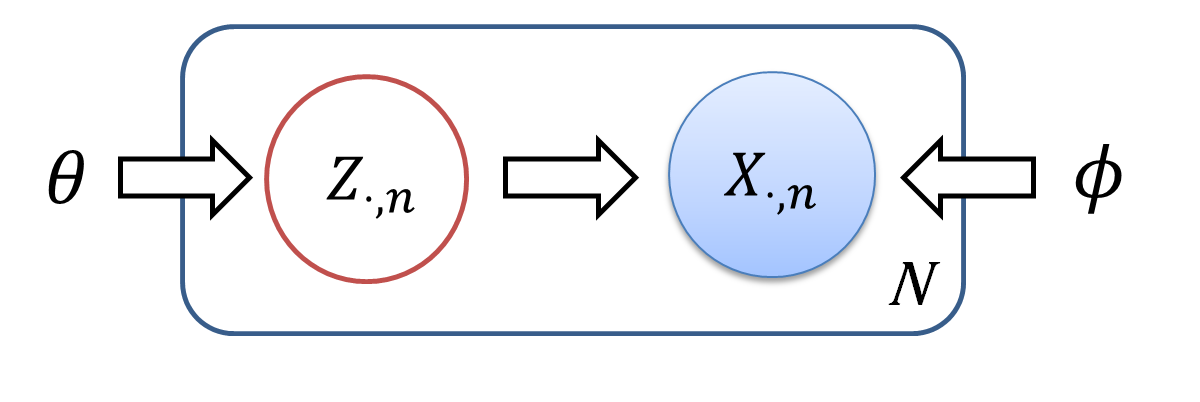
\includegraphics[width=0.75\linewidth, height=2.8cm,
        trim=0cm 0.2cm 1cm 0cm]{FIGURES/GMM}
        \caption{Plate representation for GMM }
    %\vspace{-8mm}
    \end{subfigure}
    \begin{subfigure}[H]{0.8\textwidth}
        \centering
        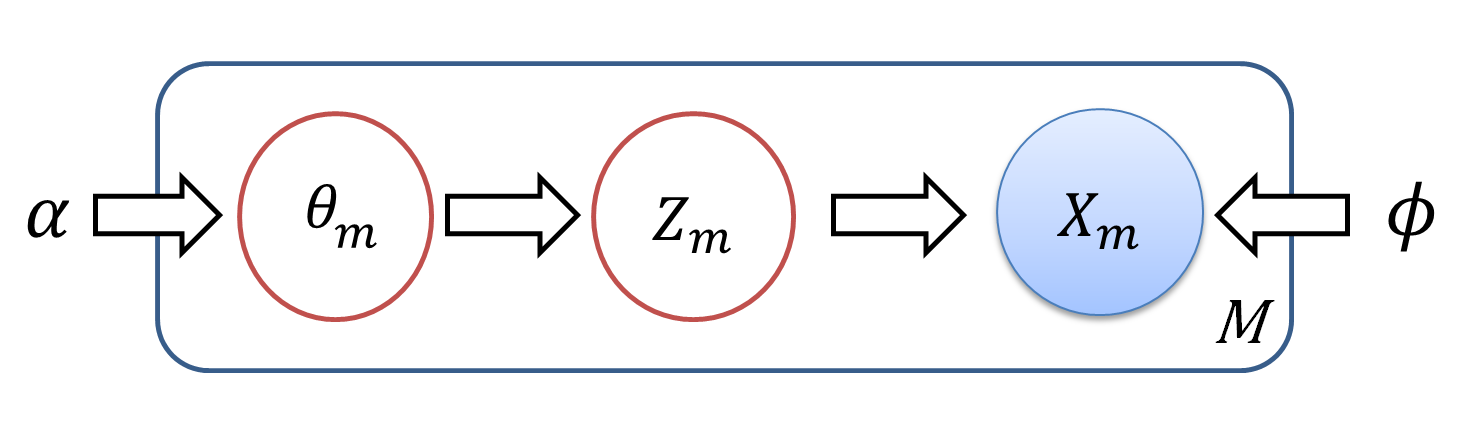
\includegraphics[width=0.9\linewidth, height=3.2cm,
        trim=0cm 0.5cm 1.2cm 0cm% height=1.2in0.75\textwidth% height=1.2in
        ]{FIGURES/LDA}
        \caption{Plate representation for LDA }
       % \vspace{-1.2cm}
    \end{subfigure}% ~   
    \caption{ Plate representation for  Gaussian Mixture Model (GMM) and Latent Dirichlet Allocation (LDA).
Shaded blue circles are observations, circles with red outlines are latent variables and symbols without circles are model parameters. %The blue rectangular plate represents  model is inferred at   particular structural level.
     }
     \label{Fig:GMMvsLDA} 
\end{figure*}

 

\subsection{ Mixture of Gaussian Mixtures (MGM)} 
 To overcome shortcomings of LDA, MGM is proposed by   Xiong et al. \cite{MGM} for distinguishing multiple types of group behaviours. % where MGM refers to Mixture of Gaussian Mixtures whilst for discrete features MGM is the Multinomial Genre Model.
  MGM is an adaptation of  Theme Topic Mixture Model  %proposed by  Keller  and Bengio 
  \cite{TTMM}  where instead of discrete datasets, MGM is constructed for continuous real-valued input data.  The MGM model introduces genres (themes) as mixtures of topics where each document is associated with certain genres.   %assumes% a group is a collection of documents where 
%  group memberships (collection of documents) are known a priori. 
  For example, books are naturally classified in terms of genres such as sci-fiction, romance, thriller and so on. Given a particular genre (type of regular behaviour), an anomalous group is characterised by an irregular mixture of topics.  %For $M$ groups, the $m$th group is specified by random vectors $ {\bf G}_{m}=\big\{ X_{mn}  \big\}_{n=1}^{N_m} $. 


In MGM, a document is  categorised by one of $J$ genres and a word in a document is generated from one of $K$ topics.   More specifically, the $m$th document is associated with latent variables such as genres $\chi_{m}$, genre mixtures $\theta_{m}$ and topics $Z_m$. 
The distributional parameters for topics, words and genres are respectively denoted with $\alpha,\phi,\gamma$.  
 The  posterior distribution in Equation  (\ref{pos})   for MGM is expressed as %   ${\bf X}= \{{\bf G}_{m},\dots,{\bf G}_{M} \} $ and model parameters are $\Theta=\{\alpha,\phi,\gamma\}$. 
 \begin{align*}
& \mbox{Observed Data:  \;\; \quad}  {\bf X}= \{{\bf G}_{1},{\bf G}_{2},\dots,{\bf G}_{M} \}\\
 & \mbox{Latent Variables: \quad}    \mathcal{H}=\{\chi_{m},\theta_m, Z_{m} \}_{m=1}^M  \\
 & \mbox{Model Parameters: \;\,}  \Theta=\{\alpha,\phi,\gamma\}
 \end{align*} 
  where ${\bf G}_{m} = \{ X_{mn} \}_{n=1}^{N_{m}}$ represents a group as a collection documents.  
  

We emphasise that in MGM, $  X_{mn} $ represents the $n$th document in the $m$th group rather than the LDA definition of the $n$th word in the $m$th document.   MGM is useful for modelling multiple groups of documents whereas a single document is a group of words for LDA.  
The MGM model also effectively learns multiple types of regular group behaviours however it may  fail to detect   point-based group anomalies  as it does not capture uncertainty of topic-word distributions. Without   Dirichlet prior distributions on topic-word probabilities in MGM, individual anomalies (specific anomalous documents) are poorly detected. 
 
 
 

\subsection{ Flexible Genre Model (FGM) }
 Xiong et al. \cite{FGM} extend MGM in a method called Flexible Genre Model (FGM).  Similar to MGM, multiple regular group behaviours are considered where a group or collection of documents is characterised by its topic  mixtures given a specific genre.  In addition, FGM  incorporates the uncertainties  of topic-word probabilities.   Dirichlet prior distributions in FGM account for  local document  structures as well as global group information  when estimating the topic-word probabilities.   This results in a better detection of point-based group anomalies as compared to MGM. 
 The topic-group weights are generated from a Dirichlet prior when data is discrete and Gaussian-Inverse-Wishart distributions for continuous real-valued datasets.
 
 Figure (\ref{Fig:FGM}) illustrates the graphical structure of FGM. MGM has a similar representation however it does not include Dirichlet priors on topic-word probabilities with $\phi_m \sim Dir(\beta)$. %With  additional Dirichlet priors,
  The posterior distribution for FGM is similar to MGM  except for additional latent variables  $\{ \phi_m\}_{m=1}^M$ and model parameters in FGM with $\Theta=\{\alpha,\beta,\gamma\}$ rather $\Theta=\{\alpha,\phi,\gamma\}$ in MGM. %For an appropriate comparison with MGM, FGM is also formulated for continuous real-valued data however it can also be adapted for discrete or categorical data.
     Overall, FGM is more effective than LDA and MGM for modelling multiple types of regular group behaviour as well as detecting point-based and distribution-based group anomalies. 

 
\begin{figure}[H]
\centering
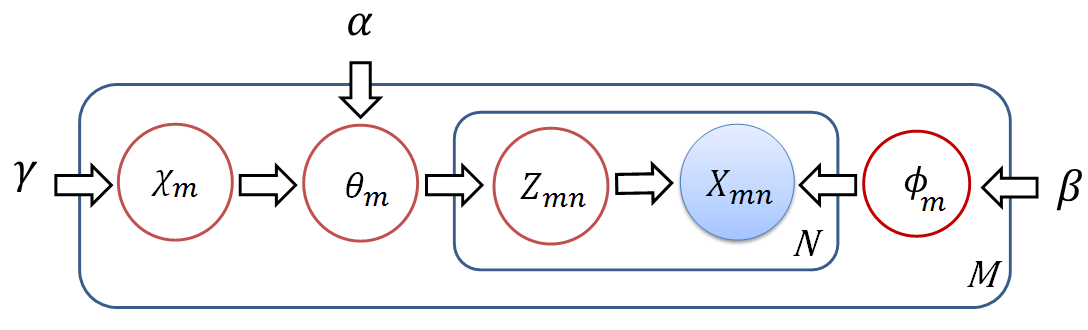
\includegraphics[width=14cm, height=4cm,trim=0cm 0cm 0cm 0.4cm]
{FIGURES/FGM} 
\caption{Graphical Representation of FGM where shaded blue circles contain observed data, unfilled  circles with red outlines are latent variables and symbols without circles are model parameters.}
%\vspace{-2cm}
\label{Fig:FGM}
\end{figure}
  

\section{Generative Models for Unknown Group Memberships}
We now elaborate on details of generative models where group memberships are unknown.   Clustering data instances into groups introduces an additional layer of  uncertainty and may not represent true group structures. Halkidi et al. \cite{ClusterValidity} discuss issues with the validity of clustering techniques %and F\~{a}rber et al. \cite{ClusterEval}  highlight that group labels may not even correspond to natural clustering structures.  
so a careful evaluation and interpretation of inferred clusters is required. % when true group memberships are unknown.
 To reduce the uncertainty of clustering data instances, Group Latent Anomaly Detection (GLAD) model \cite{GLAD} incorporates additional information from pairwise connections between data instances. %Yu et al. \cite{GLAD} find that the GLAD model has a relatively higher accuracy for inferring clusters given pointwise and pairwise data.
  Yu et al. \cite{GLAD} demonstrate the effectiveness of  GLAD in grouping data points compared to a number of graph-based clustering algorithms.



\subsection{ Group Latent Anomaly Detection (GLAD)} \label{subs:GLAD}
Detecting group anomalies becomes more challenging when memberships of groups are not previously known.  The  hierarchical structure  of GLAD utilises a combination of LDA as previously discussed and Mixed Membership Stochastic Blockmodel (MMSB) from Airoldi et al.  \cite{MMSB} to account for pairwise relationships between data points.  Similar to previous generative models, the $m$th group  is characterised by  topic proportions $\theta_{m}$ and an anomalous group is characterised by irregular topic proportions. % Yu et al. \cite{GLAD} demonstrate the effectiveness of  GLAD in clustering and  discovering group anomalies compared to a number of graph-based clustering algorithms.
A general drawback of the GLAD model is its input requirements of pairwise connection information that may not be readily available. 

The  graphical structure for the GLAD model illustrated in Figure \ref{Fig:GLAD} is noticeably different to FGM in Figure \ref{Fig:FGM}. Firstly without  prior distributions on topic-word probabilities $\phi_m$, GLAD may not be suitable for detecting point-based group anomalies. Also topic mixtures $\theta$ do not have prior distributions such that overfitting may occur if a large number of topics are examined. Compared to FGM and MGM, GLAD   does not account for multiple types of group behaviour. % Algorithm 3 further describes the  generative process of GLAD where
In Figure \ref{Fig:GLAD}, 
  ${\tilde G}_{n}$ represents a group membership indicator for the $n$th document with group membership  probability $\pi_n$. Topic variables $Z_n$ are inferred for each data point given their group membership.    The blockmodel parameter $\bf B$ contains  probabilities that documents in different groups share a connection. % one group has a connection with a document from another group. 
GLAD assumes discrete feature data  $ X_{n}$ and pairwise connections $Y_{n n'} \in \{0,1\}$  are respectively generated by  multinomial and Bernoulli distributions. Bernoulli probabilities represent the probability that there is a connection between the $n$th and $n'$th document. 

 The  posterior distribution %in Equation  (\ref{pos})   
$p({\bf X},\mathcal{H}| \boldsymbol\Theta) $ 
 for GLAD has %is summarised as %   ${\bf X}= \{{\bf G}_{m},\dots,{\bf G}_{M} \} $ and model parameters are $\Theta=\{\alpha,\phi,\gamma\}$. 
 \begin{align*}
& \mbox{Observed Data:  \;\; \quad}  {\bf X}= \{{\bf X}_{n} \}_{n=1}^N \mbox{ and } {\bf Y} =\{Y_{nn'}: 1 \le n,n' \le N \} \\
 & \mbox{Latent Variables: \quad}    \mathcal{H}=\{\pi_{n},\tilde{G}_n, Z_{n} \}_{n=1}^N  \\
 & \mbox{Model Parameters: \;\,}  \Theta=\{\eta,{\bf B},\theta, \phi\}
 \end{align*} 
  where the $n$th document is associated with one of $M$ groups with $\tilde{  G}_{n}  \in \{1,2,\dots,M\}$. 
  


 
\begin{figure}[H]
\centering
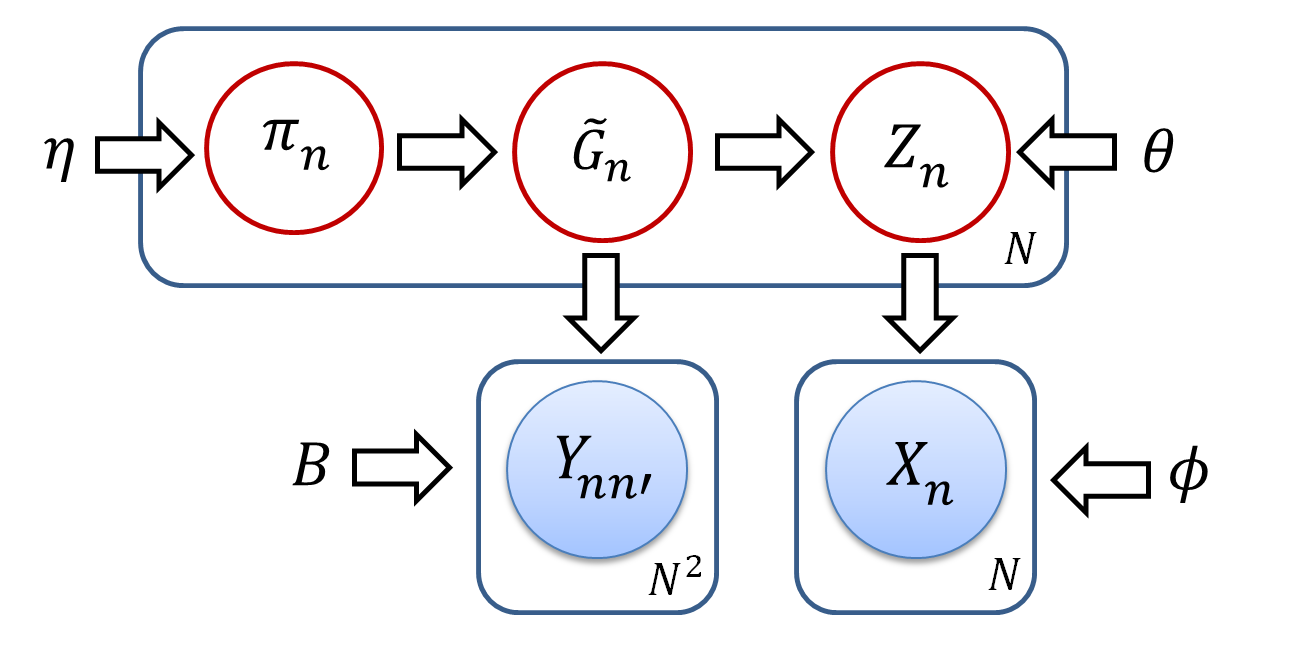
\includegraphics[width=12cm, height= 6cm,trim=0cm 0.6cm 2.5cm 0cm]
{FIGURES/GLAD} 
\caption{Graphical representation of GLAD where shaded blue circles represent observed data, circles with red outlines are latent variables and symbols without circles are model parameters.}
%\vspace{-2cm}
\label{Fig:GLAD}
\end{figure}


%\begin{landscape}
 \begin{table*}[H]
\begin{center}
 \scalebox{0.95}{
\begin{tabular}{ ccp{45mm}p{45mm}p{45mm}p{45mm}} 
 \hline\\%[-4mm]
Method & Data Variables $\bf X$ & Model Parameters $\Theta$ & Strengths & Weakness   \\%[1mm]
 \hline\\%[-4mm]
 LDA & $X_{m,n}$ &  $\alpha, \phi$ & Topic representation & Single topic mixture \\
 MGM & ${\bf G}_{m} $ %=\{X_{m,n} \}_{n} $
    & $\alpha, \phi,\chi$ & Multiple types of group behaviour & Cannot detect pointwise anomalies \\
  FGM & ${\bf G}_{m} $  & $\alpha, \beta,\chi$ & detect pointwise anomalies & Complex model \\
  ATD &  ${\bf X}_{m}  $   & $ beta, \phi$ & Incorporates sparse topic variables &  Requires labeled data \\
 %\multirow{2}{*}{GLAD} 
 GLAD & ${\bf X}_{m},{\bf Y}_{m} $   & $\alpha, beta, \psi, B$ & Simultaneously infers groups and detects anomalous groups &  Requires connection data \\
 %  OCSMM &  Group observations are IID  & Flexible representation of group behaviours. Does not require domain knowledge. & Choice of the kernel $k$. Sensitive to the parameter $\nu$ for the expected number of anomalous groups.\\
% KNNG-$\mathcal{D}$ &  Static & KNNG is nonparametric & No interpretation of anomalous group behaviour & \\ 
% MQCC & Dyanmic & Group observations are IID.
% Groups are independent over time. &  Requires training data\\
 %LRT & Dynamic & Group observations are IID.
% Groups are independent over time.  & & 
 \\ \hline
\end{tabular}
}
\end{center}
 \caption{Summary of Different Methods}
 \label{Tab:MH}
\end{table*}

%\end{landscape}


\section{Hypothesis Tests} 
\label{Sec:H}
 A hypothesis test is a specific type of generative model based on a null hypothesis or an assumption about how the data is generated. Instead of only computing a score such as in generative models, hypothesis tests also classify group deviations.  Hypothesis tests evaluate the statistical significance of an observed group with  a test statistic that captures the deviation of group observations from expected values. A statistical threshold is selected from the quantiles of a null distribution (assumed distribution following the null hypothesis).   The degree of anomalous behaviour in a group is quantified by a $p$-value or the likelihood that a group  observation is consistent with the null hypothesis. When multiple hypotheses are evaluated,  $p$-values require additional adjustment. 

 Many previous hypothesis tests have involved evaluating the equality of two groups in terms of different statistical properties. The equality of two groups has been evaluated using univariate means  in Student t-test,  multivariate mean vectors for Hotelling's $T^2$ test and univariate variances in  Barttlet's test.  There are also hypothesis tests involving more general properties such as empirical distributions in Kolmogorov-Smirnov test \cite{KStest}, multiple quantiles of two independent groups in Wilcox \cite{Wilcox1995} and quantiles of group difference distribution in Wilcox and Erceg-Hurn \cite{Wilcox2012}. The equality of multiple groups (greater than two groups) has also been studied for statistical properties such as multivariate mean vectors in MANOVA \cite{borgen1978uses},  count proportions in Chi-square test \cite{kass1980exploratory}  and covariance matrices in Box's test \cite{box1954some}. The above hypothesis tests are more effective for testing the equality of groups  however  do not explicitly classify anomalous  group behaviours. % but rather determine if there is a difference in group behaviours. 
 
 
%\begin{center}
%{\bf Advantages and disadvantages of  hypothesis testing}\\ 
%Advantages:
%\begin{enumerate}[(1)]   \setlength\itemsep{5pt}
%\item Flexible formulation  of how data is generated 
%\item Offers clear interpretation of results 
%%\item  Directly classifies group behaviours as regular or anomalous
%\item Quantifies the statistical significance of a group   
%%\item    Can be applied in a supervised or unsupervised manner % group anomaly detection
%\end{enumerate} 
%Disadvantages:
%\begin{enumerate}[(1)]   \setlength\itemsep{5pt}
%\item    Assume data follows a particular distribution under the null hypothesis 
%%\item  Results are sensitive to initial parameter  selection  
%\item Prone to overfitting for multiple hypotheses
%\end{enumerate} 
%\end{center}

 
\subsection{Anomalous Topic Detection (ATD)} \label{Sec:ATD}
In the context of topic modelling,  Soleimani \& Miller \cite{ATD} introduce  Anomalous Topic Discovery (ATD), a supervised learning approach that clusters anomalous
documents when memberships are previously unknown. The regular behaviours of documents are extracted from an appropriate training set with discrete data inputs. ATD implements a non-parametric bootstrap sampling procedure to  evaluate the statistical significance of a detected anomalous behaviour for a single document as well as a cluster of documents.     
Like in previous analysis, groups are  characterised by topic variables however an anomalous group is not characterised by irregular topic proportions. Instead  a group anomaly in ATD  is defined as a cluster with an additional topic that is not explained by  regular topics inferred from a training set.   


ATD learns topics using  Parsimonious Topic Model (PTM) proposed by Soleimani \& Miller  \cite{PTM}. % as PTM has many advantages over the simpler LDA model. 
%From Soleimani \& Miller  \cite{PTM}, 
PTM is more effective than the simpler LDA model for handling sparse topic representations in high-dimensional datasets by  incorporating  globally shared topics as well as topic-specific variables.   
  Rather than estimating  parameters through  Monte Carlo simulations or variational inference,  PTM  reduces computational burden by selecting models based on comparing information criteria.     
After clustering documents based on  topics  inferred from PTM, the ATD method evaluates the statistical significance of an anomalous cluster using a non-parametric bootstrap approach.  Figure \ref{Fig:ATD} summarises the clustering process and significance testing of anomalous documents in ATD.  %It is possible to apply other generative models such as LDA or MGM in the ATD method in order to classify groups with statistical significance rather than calculate group deviation scores. 
 
If we assume $K$ regular topics are inferred from a training set then ATD evaluates a cluster $\mathcal{C}$ based on the following hypothesis :
\begin{align}
&\mbox{ $H_0:$ Cluster $\mathcal{C}$ has $K$  regular topics } %\nonumber \\
 \mbox{ \, versus \, $H_1:$ Cluster $\mathcal{C}$ contains  $K+1$ topics }
\label{Hyp:ATD} 
\end{align}
where an additional topic is seen as anomalous. 

We explain details of ATD using the four key components from Section \ref{Sec:Problem}. 
\begin{enumerate}[1.]
\item Characterisation function $f_1({\bf G}_{train})=l_0(\mathcal{C})$: \\ 
ATD estimates $K$ regular topics and other  parameters  of a null model under $H_0$  from  training set ${\bf G}_{train}$.  
 %A hypothesis test in ATD evaluates whether  is appropriate for a test cluster. 
%This null model characterises the training set by  $K$ regular topics. 
The probability that a cluster $\mathcal{C}$ is generated under null hypothesis $H_0$  is denoted by 
$l_0(\mathcal{C}) = \sum_{n  \in \mathcal{C} } \ln p( n| H_0 ) $. 
\end{enumerate}
%
\begin{enumerate}[2.]
\item Characterisation function $f_2({\bf G}_{test})=l_1(\mathcal{C})$: \\
%We do not fully elaborate on the details of PTM, but rather focus on the ATD method. 
  Figure \ref{Fig:ATD} illustrates the process of inferring a significantly anomalous cluster with the maximum deviance  from the null hypothesis $H_0$.  
%   the ATD method for aggregating data instances into a test cluster and evaluating the presence of additional anomalous topics. % ATD is a supervised method where  regular  topics is inferred from a training set. 
 Anomalous documents from a test set  are  iteratively added to a test cluster $\mathcal{C}$ until  no  statistically significant anomalous topics are detected.   %A test cluster is then evaluated for $|\mathcal{C}|>4$.
  A test set ${\bf G}_{test}=\mathcal{D}'$ is updated by omitting the anomalous cluster where $\mathcal{C}$ is characterised by $K+1$ possible topics under hypothesis $H_1$. The likelihood  that a test cluster contains an additional topic is $l_1(\mathcal{C}) = \sum_{n \in \mathcal{C} } \ln p(n | H_1 )$. 
 %Documents with significantly anomalous behaviours are added to a test cluster in an iterative process.  
%   A test cluster  $\mathcal{C}$ requires at least 4 documents () before evaluating its anomalous behaviour.  %Similar to previous generative models, a test cluster  is a collection of documents where each document is characterised by topics. %  Since an anomalous cluster is previous unknown, naive search would take $2^{|\mathcal{D}^t|}$ subsets of a test set. 

% ATD finds a cluster $\mathcal{C}$ with  maximum deviance from the null hypothesis by the iterative process portrayed in Figure \ref{Fig:ATD}. 
%This likelihood is treated as an anomalous score. 
\begin{figure}[h]
\centering
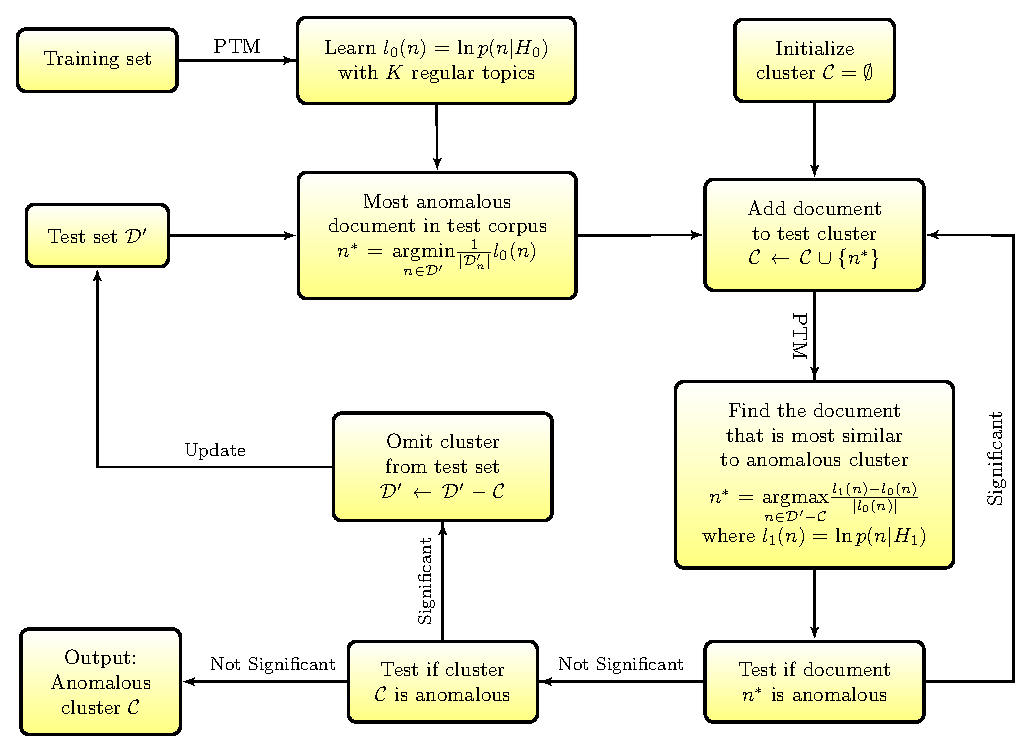
\includegraphics[width=14cm, height=10cm, trim=0cm 0cm 0cm 0cm]
{FIGURES/ATDfigure} 
\caption{ Illustration of the clustering procedure using Anomalous Topic Discovery (ATD)  }
%\vspace{-2cm}
\label{Fig:ATD}
\end{figure}

\end{enumerate}
%
\begin{enumerate}[3.] 
\item Measure $ \mathcal{D}\big(f_1 ({\bf G}_{train}) , f_2({\bf G}_{test} )\big )= l_1(\mathcal{C})  -l_0(\mathcal{C})$: \\
An anomalous score for a test cluster $\mathcal{C}$ is computed by the log-likelihood ratio  
\[\mathcal{S}(\mathcal{C})= l_1(\mathcal{C})  -l_0(\mathcal{C}) =   \sum_{n  \in \mathcal{C} } \ln \frac{p( n| H_1 )} {p( n| H_0 )} \]
which quantifies the probability that a cluster contains a significantly different topic from $K$ regular topics inferred from  training data. Other generative models only calculate group deviation scores however ATD also evaluates the statistical significance of a test cluster. 
% An anomalous measure  is calculated by a $p$-value or likelihood that a test cluster is consistent with the null hypothesis. A parametric distribution for group deviation scores is not assumed as clusters may have small sample sizes. % as $|\mathcal{C}|>4$. 
  A non-parametric bootstrap procedure is  applied  where the null distribution is estimated by sampling documents from the  training set.  Scores for $B$ bootstrap clusters are respectively denoted by    $\mathcal{S}(\mathcal{C}_1),\mathcal{S}(\mathcal{C}_2),\dots,\mathcal{S}(\mathcal{C}_B)$ and an empirical $p$-value for test cluster scores is calculated by    
\[ \frac{1} {B+1} \sum_{b=1}^B \Big[I \Big(b : \mathcal{S}(\mathcal{C}_b) > \mathcal{S}(\mathcal{C}) \Big)+1 \Big] \]
where $B$ is the number of bootstrap simulations. 
  Further details of bootstrapping procedures for ATD are described in Soleimani \& Miller \cite{ATD}. 
\end{enumerate}
\begin{enumerate}[4.]
\item Threshold $\epsilon=\alpha$: \\ 
Once a $p$-value is calculated, a statistical threshold is selected from the quantiles of the null distribution generated from bootstrap simulations. 
Soleimani \& Miller \cite{ATD} do not describe multiple hypothesis testing issues for iteratively evaluating   anomalous documents or test clusters. Thus a  test cluster is considered anomalous if the empirical $p$-value is less than a pre-selected  significance level $\alpha$. 
\end{enumerate}
 
 
\subsection{Extreme Rank Anomalous Collection Detection (ERACD)}
Dai et al. \cite{ERACD} introduce Extreme Rank Anomalous Collection Detection (ERACD), an unsupervised approach that evaluates the statistical significance of  inferred clusters % collections of data instances 
 where group memberships are previously unknown. ERACD aggregates data instances into anomalous clusters based on extreme rankings. Group anomalies are characterised by a variety of extreme features such that multiple hypotheses evaluate the significance of group deviations. % and evaluated using a Bonferroni correction method \cite{Bonferroni}. 
The ERACD  algorithm detects both a point-based group anomaly as a large number of entities with a single extremely ranked feature or a distribution-based group deviation where entities have extreme ranks across multiple features.

ERACD has many advantages over other state-of-the-art methods. 
The ERACD  algorithm focuses on a relatively small number of members in clusters whereas many other methods require larger group sizes. Dai et al. \cite{ERACD} find that ERACD infers clusters with more anomalous behaviours compared to other clustering techniques.  Hypothesis tests in ERACD also provide an explanation for the deviating statistical properties of a group anomaly. % based different assumptions of independent and dependent feature sets.  
ERACD requires model parameters such as the number of expected anomalous clusters and the maximum allowable size for clusters.  % Model selection in ERACD is difficult  to automate and evaluate without sufficient labeled data. 
  The effectiveness and interpretation of results is sensitive to initial parameter selection.   
 %Due to the flexible framework of ERACD, it can be applied to networks data where feature data for a particular node is obtained by the path distance to different entities in a cluster. 

  Since the detection of distribution-based anomalous clusters across multiple features requires more elaborate details, we describe key components of ERACD for detecting point-based group anomalies as follows.  
A general hypothesis involving the $v$th feature of a test cluster $\mathcal{C}$ can be stated as 
\begin{align}
&  \mbox{ $H_0:$  $v$th feature of cluster $\mathcal{C}$ is regular}  \mbox{ \, versus \, $H_1:$  $v$th feature of cluster $\mathcal{C}$ is anomalous   }
\label{Hyp:ERACD} 
\end{align}
where multiple hypotheses are evaluated over different  statistical properties with features $v=1,\dots, V$.  

\begin{enumerate}[1.]
\item Characterisation function $f_1({\bf G}_{train})=|{\bf X}_{v} (r)|$: \\ 
%The entities that contains extreme features is  an extremity index $r$ 
Consider $N$ data instances each with $V$ features where the rank of feature $v$ for the $n$th data instance is denoted by $rank_v(n)$ for $n=1,2,\dots,N$. 
Based on the $v$th feature, data instances in the training set
 $\bf X$ with  top $r$ rank positions (highest values) are examined according to  
\begin{align}
{\bf X}_{v} (r) = \{n |n \in  {\bf X}, \, rank_v(n) \le r \} \label{Eqn:Rank}
\end{align} 
ERACD characterises the training set by the number of elements  with $|{\bf X}_{v} (r)|$. 
%Since ties may occur in a dataset, it is possible that the $n$th and $n'$th instance have $rank_v(n)=rank_v(n')$. Generally
with  the $r$th rank  of feature $v$ satisfying   $ | {\bf X }_{v} (r) | \le r$. 
 %Rather than examining regular behaviours in training data,
 The function $f_1$ characterises regular behaviour of a training data for  extreme ranks of features.   

\end{enumerate}

\begin{enumerate}[2.]
\item Characterisation function $f_2({\bf G}_{test}) = |{C}_{v} (r)|$: \\ 
ERACD  algorithm infers group structures using an iterative pruning technique based on anomaly scores.  The  top $r$ rank positions of the $v$th feature for cluster $\mathcal{C}$  is given by 
\begin{align}
{C}_{v} (r) = \{n |n \in \mathcal{C}, \, rank_v(n) \le r \} \label{Eqn:Rank}
\end{align} 
Similarly, ERACD characterises a test set by the number of elements in a test cluster   with $|\mathcal{C}_{v} (r)|$. 
%By only examining a single feature, point-based group anomalies are detected however distribution-based anomalous clusters are discovered based on extreme ranks across multiple features.  
\end{enumerate}


\begin{enumerate}[3.] 
\item Measure $ \mathcal{D}\big(f_1 ({\bf G}_{train}) , f_2({\bf G}_{test} )\big ) = {p}_v(\mathcal{C},r^*)$: \\
Cluster ${C}_{v} (r)$ is compared with $ { \bf X}_{v} (r) $ to  identify point-based anomalous clusters for the $v$th feature. 
%To test if an inferred cluster is anomalous with respect to its $v$th feature,
 The null hypotheses in ERACD assumes that  randomly selecting  entities (with top ranked features)  in a collection $\mathcal{C}$ as compared to the whole dataset $\bf X$ follows a  hypergeometric distribution. 
A hypergeometric probability with parameters $a,b,c,d $ is given by
\begin{align}
 P(a,b,c,d) = \displaystyle \frac{ {a+b \choose{a} } { c+d \choose{c} } } { {N' \choose{a+c} } } \label{Eqn:hyperG}
\end{align} 
where the total count is $N' = a+b+c+d$. 
  If a group is characterised by top $r$ ranks of feature $v$, a $p$-value is calculated from the upper tail with  
 \[           p_v( \mathcal{C} ,r ) =  
 \displaystyle \sum_{n = |\mathcal{C}_v (r) | |} ^ {\min(| {\bf X}_v (r) |,| \mathcal{C}| )}  P (n, N,|{\bf X}_{v}  (r)|,|\mathcal{C}| ) \]
where probabilities are given by the hypergeometric distribution  in Equation (\ref{Eqn:hyperG}). In practice, the selection of parameter $r$ is difficult and Dai et al. \cite{ERACD}  define a representative value with   
%\begin{align}
$r^* = \underset { 0 < r < N/2 } { \mbox{argmin}} \,  p_v( \mathcal{C} ,r )$ % \label{Eqn:RepInd}
%\end{align}
For a particular feature,  a representative $p$-value $p_v( \mathcal{C} ,r^* )$  is a more appropriate measure for  extremely ranked behaviour of a cluster, compared to using $p$-values with a different value of $r$. %entities with extreme ranks from training data.  
   
\end{enumerate}
\begin{enumerate}[4.]
\item Threshold $\epsilon=\alpha/V$: \\ If a single hypothesis is evaluated for an inferred cluster  then a $p$-value is significant if it is less than  a pre-defined significance level  $\alpha$. Since ERACD evaluates $V$ hypothesis to search for features that characterise anomalous clusters,  a Bonferroni adjustment \cite{Bonferroni}  is applied where a test cluster  is anomalous if % it has a $p$-value less than the following threshold
\[  {p}_v(\mathcal{C},r^*) < \alpha/V \]   
\end{enumerate}




%% Chapter-2 Supervised DAD
% Supervised DAD-1
\chapter{Supervised Deep Anomaly Detection Methods}
\label{chpt:supervisedDAD}
\section{Introduction}
Pharmacovigilance (PV) is defined by the World Health Organization as the science and activities concerned with the detection, assessment, understanding and prevention of adverse effects of drugs or any other drug-related problems. Drug name recognition (DNR) is a fundamental step in the PV pipeline, similarly to  the well-studied Named Entity Recognition (NER) task for general natural language processing (NLP). DNR aims to find drug mentions in unstructured biomedical texts and classify them into predefined categories in order to link drug names with their effects and explore drug-drug interactions (DDIs). Conventional  approaches to DNR sub-divide as rule-based, dictionary-based and machine learning-based. Intrinsically, rule-based systems are hard to scale, time-consuming to assemble and ineffective in the presence of informal sentences and abbreviated phrases. Dictionary-based systems identify drug names by matching text chunks against drug dictionaries. These systems typically achieve high precision, but suffer from low recall (i.e., they miss a significant number of mentions) due to spelling errors or drug name variants not present in the dictionaries~\cite{liu2015drug}. Conversely, machine-learning approaches have the potential to overcome all these limitations since their foundations are intrinsically robust to variants. The current state-of-the-art machine learning approaches follow a two-step process of feature engineering and classification~\cite{segura2015exploring,abacha2015text,huber2013wbi}. Feature engineering refers to the task of representing text by dedicated numeric vectors using domain knowledge. Similarly to the design of rule-based systems, this task requires much expert knowledge, is typically challenging and time-consuming, and has a major impact on the final accuracy. For this reason, this paper explores the performance of contemporary recurrent neural networks (RNNs) at providing end-to-end DNR straight from text, without any manual feature engineering stage. The tested RNNs include the popular Elman and Jordan networks and the bidirectional long short-term memory (LSTM) with decoding provided by a conditional random field (CRF)~\cite{elman1990finding,jordan1986serial,lample2016neural,collobert2011natural}. The experimental results over the SemEval-2013 Task 9.1 benchmarks show an interesting accuracy from the LSTM-CRF that exceeds that of various manually-engineered systems and approximates the best result in the literature.

% !TEX root=../main.tex
\section{Related Work}
\label{supervisedDAD:RelatedWork}
Most of the research on drug name recognition to date has focussed on domain-dependent aspects and specialized text features. The benefit of leveraging such tailored features was made evident by the results from the SemEval-2013 Task 9.1 (Recognition and classification of pharmacological substances, known as DNR task) challenge. The system that ranked first, WBI-NER~\cite{huber2013wbi}, adopted very specialized features derived from an improved version of the ChemSpot tool~\cite{rocktaschel2012chemspot}, a collection of drug dictionaries and ontologies. Similarly, many other recent approaches~\cite{abacha2015text,liu2015feature,segura2015exploring} have been based on various combinations of general and domain-specific features. In the broader field of machine learning, the recent years have witnessed a rapid proliferation of deep neural networks, with unprecedented results in tasks as diverse as visual, speech and named-entity recognition \cite{hinton2012deep,krizhevsky2012imagenet,lample2016neural}. One of the main advantages of neural networks is that they can learn the feature representations automatically from the data, thus avoiding the laborious feature engineering stage~\cite{mesnil2015using,lample2016neural}. Given these promising results, the main goal of this paper is to provide the first performance investigation of popular RNNs such as the Elman and Jordan networks and the bidirectional LSTM-CRF over DNR tasks.

% !TEX root=../main.tex
\section{The Proposed Approach}
\label{sec:method}
\begin{table*}[ht]
    \small
    \centering
    \scalebox{0.9}{
        \begin{tabular}{|c|c|c|c|c|c|c|c|c|c|}
            \hline \bf Sentence & \textit{Cimetidine}& \textit{reduces} & \textit{clearance}& \textit{of} & \textit{ALFENTA} &\textit{and} &\textit{volatile} &\textit{inhalation} &\textit{anesthetics}  \\
            \hline \textbf{Entity class}& \textit{B-drug}& \textit{O}& \textit{O} & \textit{O}& \textit{B-brand} & \textit{O} & \textit{B-group } & \textit{I-group} & \textit{I-group}  \\
            \hline
        \end{tabular}}
        \caption{Example sentence in a DNR task with entity classes represented in IOB format.}
        \label{table1}
\end{table*}

\begin{table*}[ht]
    \centering
    \scalebox{0.9}{
    \begin{tabular}{|c|c|c|c|c|}
        \hline
        \multirow{3}{*}{} &
        \multicolumn{2}{c|}{\bf {\small DDI-DrugBank}} &
        \multicolumn{2}{c|}{\bf {\small DDI-MedLine}} \\
        \cline{2-5}
        \cline{2-5}
        & Training+Test for DDI task & Test for DNR & Training+Test for DDI task & Test for DNR\\
        \hline
        documents &$730$ &$54$ & $175$ & $58$ \\
        sentences &$6577$&$145$ &$1627$  & $520$\\
        \hline
        drug\_n  & $124$   & $6$ &  $520$ & $115$ \\
        group&  $3832$ & $65$&  $234$ & $90$\\
        brand& $1770$ & $53$ &  $36$ & $6$\\
        drug&  $9715$ & $180$& $1574$ & $171$\\  \hline
    \end{tabular}}
    \caption{Statistics of training and test datasets used for SemEval-2013 Task 9.1.}
    \label{table2}
\end{table*}

DNR can be formulated as a joint segmentation and classification task over a predefined set of classes. As an example, consider the input sentence provided in Table~\ref{table1}. The notation follows the widely adopted in/out/begin (IOB) entity representation with, in this instance, \textit{Cimetidine} as the drug, \textit{ALFENTA} as the brand, and words \textit{volatile inhalation anesthetics} together as the group. In this paper, we approach the DNR task by recurrent neural networks and we therefore provide a brief description hereafter. In an RNN, each word in the input sentence is first mapped to a random real-valued  vector of arbitrary dimension, $d$. Then, a measurement for the word, noted as $x(t)$, is formed by concatenating the word's own vector with a window of preceding and following vectors (the "context''). An example of input vector with a context window of size $s = 3$ is:

\vspace{-0.7 cm}

\begin{equation}
\begin{split}
w_{3}(t) = [Cimetidine, \textbf{reduces}, effect], \\
`reduces' \rightarrow x_{reduces} \in \mathbb{R}^{d}, \\
`Cimetidine' \rightarrow x_{Cimetidine} \in \mathbb{R}^{d}, \\
`effect' \rightarrow x_{effect} \in \mathbb{R}^{d}, \\
x(t) = [x_{Cimetidine}, x_{\textbf{reduces}}, x_{effect}] \in \mathbb{R}^{3d}
\end{split}
\end{equation}

\noindent where $w_{3}(t)$ is the context window centered around the $t$-th word, $'reduces'$, and $x_{word}$ represents the numerical vector for $word$.

For the Elman network, both $x(t)$ and the output from the hidden layer at time $t-1$, $h(t -1)$, are input into the hidden layer for frame $t$. The recurrent connection from the past time frame enables a short-term memory, while hidden-to-hidden neuron connections make the network Turing-complete. This architecture, common in RNNs, is suitable for prediction of sequences. Formally, the hidden layer is described as:

\vspace{-0.4 cm}
\begin{equation}
 h(t) = f(U \bullet x(t) + V \bullet h(t-1) )
\end{equation}

\noindent where $U$ and $V$ are randomly-initialized weight matrices between the input and the hidden layer, and between the past and current hidden layers, respectively. Function $f(\cdot)$ is the sigmoid function:

\begin{equation}
f(x)=\frac{1}{1+e^{-x}}
\end{equation}

\noindent that adds non-linearity to the layer. Eventually, $h(t)$ is input in the output layer:

\vspace{-0.6 cm}

\begin{equation}
\label{eq4}
y(t) = g(W \bullet h(t)), \hspace{0.03in} \text{with} \hspace{0.03in}  g(z_{m}) = \frac{e^{z_{m}}} {\Sigma _{k=1}^Ke^{z_{k}} }
\end{equation}

\noindent and convolved with the output weight matrix, $W$. The output is normalized by a multi-class logistic function, $g(\cdot)$, to become a proper probability over the class set. The output dimensionality is therefore determined by the number of entity classes (i.e., $4$ for the DNR task).

The Jordan network is very similar to the Elman network, except that the feedback is sourced from the output layer rather than the previous hidden layer:


\begin{equation}
h(t) = f( U \bullet x(t) + V \bullet y(t-1) ).
\end{equation}


Although the Elman and Jordan networks can learn long-term dependencies, their exponential decay biases them toward their most recent inputs~\cite{bengio1994learning}. The LSTM was designed to overcome this limitation by incorporating a gated memory-cell to capture long-range dependencies within the data~\cite{hochreiter1997long}. In the bidirectional LSTM, for any given sentence, the network computes both a left, $\overrightarrow{h}(t)$, and a right, $\overleftarrow{ h}(t)$, representations of the sentence context at every input, $x(t)$. The final representation is created by concatenating them as $h(t) = [\overrightarrow{h}(t)$;$\overleftarrow{ h}(t)]$. All these networks utilize the $h(t)$ layer as an implicit feature for entity class prediction: although this model has proved effective in many cases, it is not able to provide joint decoding of the outputs in a Viterbi-style manner (e.g., an I-group cannot follow a B-brand; etc). Thus, another modification to the bidirectional LSTM is the addition of a conditional random field (CRF)~\cite{lafferty2001conditional} as the output layer to provide optimal sequential decoding. The resulting network is commonly referred to as the bidirectional LSTM-CRF \cite{lample2016neural}.

\section{Experimental Setup}  \label{sec:experiment-setup}
% !TEX root=../main.tex
\subsection{Datasets}
The DDIExtraction 2013 shared task challenge from SemEval-2013 Task 9.1~\cite{segura2013semeval} has provided a benchmark corpus for DNR and DDI extraction. The corpus contains manually-annotated pharmacological substances and drug-drug interactions (DDIs) for a total of $18,502$ pharmacological substances and $5,028$ DDIs. It collates two distinct datasets: DDI-DrugBank and DDI-MedLine~\cite{herrero2013ddi}. Table~\ref{table2} summarizes the basic statistics of the training and test datasets used in our experiments. For proper comparison, we follow the same settings as \cite{segura2015exploring}, using the training data of the DNR task along with the test data for the DDI task for training and validation of DNR. We split this joint dataset into a training and validation sets with approximately $70\%$ of sentences for training and the remaining for validation.

\subsection{Evaluation Methodology}
Our models have been blindly evaluated on unseen DNR test data using the \textit{strict} evaluation metrics. With this evaluation, the predicted entities have to match the ground-truth entities exactly, both in boundary and class. To facilitate the replication of our experimental results, we have used a publicly-available library for the implementation\footnote{\tt https://github.com/raghavchalapathy/dnr} (i.e., the Theano neural network toolkit \cite{bergstra2010theano}). The experiments have been run over a range of values for the hyper-parameters, using the validation set for selection~\cite{bergstra2012random}. The hyper-parameters include the number of hidden-layer nodes, $H \in \{25, 50, 100\}$, the context window size, $s \in \{1, 3, 5\}$, and the embedding dimension, $d \in \{50, 100, 300, 500, 1000\}$. Two additional parameters, the learning and drop-out rates, were sampled from a uniform distribution in the range $[0.05, 0.1]$. The embedding and initial weight matrices were all sampled from the uniform distribution within range $[-1, 1]$. Early training stopping was set to $100$ epochs to mollify over-fitting, and the model that gave the best performance on the validation set was retained. The accuracy is reported in terms of micro-average F$_1$ score computed using the CoNLL score function~\cite{Nadeau:07}.


\section{Experimental Results}
\label{sec:experiment-results}

Table \ref{table3} shows the performance comparison between the explored RNNs and state-of-the-art DNR systems. As an overall note, the RNNs have not reached the same accuracy as the top system, WBI-NER \cite{huber2013wbi}. However, the bidirectional LSTM-CRF has achieved the second-best score on DDI-DrugBank and the third-best on DDI-MedLine. These results seem interesting on the ground that the RNNs provide DNR straight from text rather than from manually-engineered features. Given that the RNNs learn entirely from the data, the better performance over the DDI-DrugBank dataset is very likely due to its larger size. Accordingly, it is reasonable to expect higher relative performance should larger corpora become available in the future. Table \ref{table4} also breaks down the results by entity class for the bidirectional LSTM-CRF. The low score on the $brand$ class for DDI-MedLine and on the $drug\_n$ class (i.e., active substances not approved for human use) for DDI-DrugBank  are likely attributable to the very small sample size (Table \ref{table2}). This issue is also shared by the state-of-the-art DNR systems.

% !TEX root=../main.tex
%By modeling images as group anomalies
\section{Conclusion}
\label{sec:conclusion}
This paper has investigated the effectiveness of recurrent neural architectures, namely the Elman and Jordan networks and the bidirectional LSTM-CRF, for drug name recognition. The most appealing feature of these architectures is their ability to provide end-to-end recognition straight from text, sparing effort from laborious feature construction. To the best of our knowledge, ours is the first paper to explore RNNs for entity recognition from pharmacological text. The experimental results over the SemEval-2013 Task 9.1 benchmarks look promising, with the bidirectional LSTM-CRF ranking closely to the state of the art. A potential way to  further improve its performance would be to initialize its training with unsupervised word embeddings such as Word2Vec~\cite{Mikolov:13} and GloVe~\cite{Pennington:14}. This approach has proved effective in many other domains and still dispenses with expert annotation effort; we plan this exploration for the near future.





% Supervised DAD-2
\section{Problem Introduction}
\label{sec:conceptExtraction}
Patient clinical records contain  longitudinal record of patient health, disease, test's conducted  and response to treatment, often useful for epidemiologic and clinical research. Thus extracting these information  has been of immense value for both clinical practise and to improve  quality of patient care provided  while reducing healthcare costs. Concept extraction (CE) aims to identify medical concept mentions such as problems, test, treatments in  clinical  records (Eg: discharge summaries, progress reports) and classify them into pre-defined categories. The concepts in  clinical records are often expressed with unstructured free text, rendering their extraction a daunting task for  clinical Natural Language Processing (NLP) systems. The CE  problem is analogous to well-studied Named Entity Recognition (NER) task in general NLP domain. Traditional approaches to extracting concepts relied on  rule based systems or dictionaries (lexicon's) using string comparision to recognise concepts of interest. The concepts  represent drug names, anatomical nomenclature, other specialised names and phrases which are not part of mundane English vocabulary. For instance "resp status" should be interpreted as "response status". Furthermore the use of abbreviated phrases are very common among medical fraternity and many of these abbreviations have alternative meanings in other genres of English. Intrinsically, rule based systems are hard to scale, and ineffective in the presence of informal sentences and abbreviated phrases~\cite{liu2015drug}. Dictionary based systems perform a  fast look-up  from medical ontologies such as Unified Medical Language System (UMLS)  to extract concepts~\cite{kipper2008system}. Although these systems achieve high precison but suffer from low recall ( i,e they may not identify significant number of concepts) due to missplelled words or medical jargons not present in dictionaries. To overcome these limitations various supervised and semi-supervised machine learning (ML) approaches and its variants  have been proposed utilizing conditional random fields (CRF), maximum entropy and support vector machines~(SVM) models which utilize both textual and contextual information while reducing the dependency on lexicon lookup~\cite{lafferty2001conditional,berger1996maximum,joachims1998text}. However these state-of-the-art ML approaches follow two step process of domain specific feature engineering and classification, which are highly dedicated hand-crafted systems and require labour intensive expert knowledge. For this reason, this paper employs bidirectional LSTM-CRF intialized with  general purpose off-the-shelf neural word embeddings derived from Glove~\cite{Pennington:14} and Word2Vec~\cite{Mikolov:13}  for automatic feature learning thus avoiding time-consuming feature engineering,  which deliver system performance comparable to the best submissions from the 2010 i2b2/VA challenge.

\section{Related Work}
\label{Sec:Related}

 Most of the research to date have formulated CE as a sequence labelling NER problem employing various supervised and semi-supervised ML algorithms employing focussed domain-dependent attributes and specialized text features~\cite{uzuner20112010}. Similarly hybrid models obtained by cascading CRF and SVM algorithms along with several pattern matching rules are shown to produce effective results~\cite{boagcliner}. The efficacy of including pre-processing technique (such as truecasing and annotation combination) along with CRF based NER system to improve concept extraction performace was exemplified by \cite{fu2014improving}. The best performing system for 2010 i2b2/VA concept extract task adopted unsupervised feature representations  derived from unlabeled corpora using Brown clustering technique along with semi-supervised Markov HMM models~\cite{de2011machine}. However, the unsupervised one-hot word feature representations derived from Brown clustering fails to capture multiple aspect relation between words. Subsequently~\cite{jonnalagadda2012enhancing} demonstrated that random indexing model with distributional word representations  improve clinical concept extraction. With recent success of incorporating word embeddings derived from the entire English wikipedia in various NER task \cite{collobert2011natural}, binarized word embeddings derived from domain specific copora (Eg: Monitoring in Intensive Care (MIMIC) II corpus)  has improved performance of CRF based concept extraction system~\cite{wu2015study}. In the broader field of machine learning, the recent years have witnessed proliferation of  deep neural networks, with unprecedented results in tasks such as visual, speech and NER. One of the main advantages of neural networks is that they learn features automatically thus avoiding laborious feature engineerin. Given these promising results obtained the main goal of this paper is to employ bidirectional LSTM CRF intialized with general off-the-shelf unsupervised word embeddings derived from Glove and Word2Vec models and evaluate its performance. The experimental results obtained on 2010 i2b2/VA reference standard corpora without use of any extensive feature engineering  and domain specific resources is very encouraging.



 %
 % The following footnote without marker is needed for the camera-ready
 % version of the paper.
 % Comment out the instructions (first text) and uncomment the 8 lines
 % under "final paper" for your variant of English.
 %
 % \blfootnote{
 %     %
 %     % for review submission
 %     %
 %     \hspace{-0.65cm}  % space normally used by the marker

 %     %
 %      % final paper: en-uk version (to license, a licence)


 % }

 \begin{table*}[ht]
    \small
    \centering

    \begin{tabular}{|c|c|c|c|c|c|c|c|c|c|c|c|}
        \hline \bf Sentence & \textit{His}& \textit{HCT} & \textit{had}& \textit{dropped} & \textit{from} &\textit{36.7} &\textit{despite} &\textit{2U} &\textit{PRBC} &\textit{and} &\textit{3U-FFP} \\
        \hline \textbf{Concept class}& \textit{B-test}& \textit{I-test}& \textit{O} & \textit{O}& \textit{O} & \textit{O} & \textit{ O} & \textit{B-treatment} & \textit{I-treatment} & \textit{O} & \textit{O}\\
        \hline
    \end{tabular}
    \caption{Example sentence in a CE task with concept classes represented in IOB format.}
    \label{table1}
 \end{table*}



 \begin{table*}[ht]
    \centering

        \begin{tabular}{|c|c|c|}
            \hline
            \multirow{3}{*}{} &
            \multicolumn{2}{c|}{\bf {\small 2010 i2b2/VA}} \\
            \cline{2-3}

            & Training for CE task & Test for CE \\
            \hline
            notes &$170$ &$256$  \\
            sentences &$16315$&$27626$\\
            \hline
            problem  & $7073$   & $12592$  \\
            test&  $4608$ & $9225$\\
            treatment& $4844$ & $9344$\\
             \hline
        \end{tabular}
        \caption{Statistics of training and test datasets used for 2010-i2b2 concept extraction.}
        \label{table2}
    \end{table*}


\section{Method}
\label{sec:method}
CE can be formulated as a joint segmentation and classification task over a predefined set of classes. As an example, consider the input sentence provided in Table~\ref{table1}. The notation follows the widely adopted in/out/begin (IOB) entity representation with, in this instance, \textit{HCT} as the test, \textit{2U PRBC} as the treatment. In this paper, we approach the CE task by bidirectional LSTM CRF and we therefore provide a brief description hereafter. In a bidirectional LSTM CRF, each word in the input sentence is first mapped to a random real-valued  vector of arbitrary dimension, $d$. Then, a measurement for the word, noted as $x(t)$, is formed by concatenating the word's own vector with a window of preceding and following vectors (the ``context''). An example of input vector with a context window of size $s = 3$ is:
\begin{equation}
  \begin{split}
    w_{3}(t) = [His, \textbf{HCT}, dropped], \\
    `His' \rightarrow x_{HCT} \in \mathbb{R}^{d}, \\
    `HCT' \rightarrow x_{His} \in \mathbb{R}^{d}, \\
    `dropped' \rightarrow x_{dropped} \in \mathbb{R}^{d}, \\
    x(t) = [x_{His}, x_{\textbf{HCT}}, x_{dropped}] \in \mathbb{R}^{3d}
  \end{split}
\end{equation}

\noindent where $w_{3}(t)$ is the context window centered around the $t$-th word, $'HCT'$, and $x_{word}$ represents the numerical vector for $word$.


\subsection{Word Embeddings}
Word embeddings are  dense vector  representations of natural language words that preserves the semantic and syntactic similarities between them. The vector representations could be generated by either count based such as Hellinger-PCA ~\cite{lebret2013word}, direct prediction models such as Word2Vec comprising of Skip-gram or Common Bag of Words (CBOW) or Glove word embeddings. Glove vector representations captures complex patterns beyond word similarity through by combining  efficient use of word co-occurance statistics and generate a global vector representation for any given word.

%This is achieved  through representing words as high-dimensional vectors: the spatial relationship between these vector representations subsequently  capture  the semantic relationships among words.



\subsection{Bidirectional LSTM-CRF Networks}

The LSTM was designed to overcome this limitation by incorporating a gated memory-cell to capture long-range dependencies within the data~\cite{hochreiter1997long}. In the bidirectional LSTM, for any given sentence, the network computes both a left, $\overrightarrow{h}(t)$, and a right, $\overleftarrow{ h}(t)$, representations of the sentence context at every input, $x(t)$. The final representation is created by concatenating them as $h(t) = [\overrightarrow{h}(t)$;$\overleftarrow{ h}(t)]$. All these networks utilize the $h(t)$ layer as an implicit feature for entity class prediction: although this model has proved effective in many cases, it is not able to provide joint decoding of the outputs in a Viterbi-style manner (e.g., an I-group cannot follow a B-brand; etc). Thus, another modification to the bidirectional LSTM is the addition of a conditional random field (CRF)~\cite{lafferty2001conditional} as the output layer to provide optimal sequential decoding. The resulting network is commonly referred to as the bidirectional LSTM-CRF \cite{lample2016neural}.



\begin{table*}[ht]
  \centering

    \begin{tabular}{|c|c|c|c|}
      \hline
      \multirow{3}{*}{Methods} &
      \multicolumn{3}{c|}{\bf {\small 2010 i2b2/VA}} \\
      \cline{2-4}
      & Precision & Recall & F$_1$ Score \\
      \hline
      semi-supervised Markov HMM \cite{de2011machine} &$86.88$ &$83.64$ & $85.23$ \\
      % \hline
      distributonal semantics-CRF \cite{jonnalagadda2012enhancing} &$85.60$&$82.00$ &$83.70$  \\
      binarized neural embedding CRF\cite{wu2015study}&$85.10$&$80.60$ & $82.80$ \\
      CliNER \cite{boagcliner}&$79.50$&$81.20$ & $80.00$ \\
      truecasing CRFSuite \cite{fu2014improving}&$80.83$&$7 1.47$ & $75.86$ \\
      \hline
      \bf(Our Approach) & & &  \\
      random-bidirectional LSTM-CRF &$00.00$ &$00.00$ & $78.13$ \\
      Word2Vec-bidirectional LSTM-CRF &$00.00$ &$00.00$ & $81.30$ \\
      Glove-bidirectional LSTM-CRF &$00.00$ &$00.00$ & $83.81$ \\
      \hline
    \end{tabular}
    \caption{Performance comparison between the bidirectional LSTM CRF (bottom three lines) and state-of-the-art systems (top five lines) over the 2010 i2b2/VA concept extraction task.}
    \label{table3}
  \end{table*}



\section{ Experiment Setup}
\label{Sec:experimentsetup}
\subsection{Datasets}
\label{sec:length}
The 2010 i2b2/VA Workshop on Natural Language Processing Challenges for Clinical Records presented three tasks, one among them is  concept extraction task focused on the extraction of medical concepts from patient  reports. A total of 394 training reports, 477 test reports, and 877 unannotated reports were de-identified and released to challenge participants with data use agreements~\cite{uzuner20112010}. However part of that data set is no longer being distributed due to Institutional Review Board (IRB) restrictions. Table~\ref{table2} summarizes the basic statistics of the training and test datasets used in our experiments. We split training dataset into a training and validation sets with approximately $70\%$ of sentences for training and the remaining for validation.

\subsection{Evaluation Methodology}
\label{sec:length}
Our models have been blindly evaluated on unseen 2010 i2b2/VA  CE test data using the \textit{strict} evaluation metrics. With this evaluation, the predicted entities have to match the ground-truth entities exactly, both in boundary and class. To facilitate the replication of our experimental results, we have used a publicly-available library for the implementation (i.e., the Theano neural network toolkit \cite{bergstra2010theano}) and we publicly release our code\footnote{\hspace{-0.65cm}https://github.com/raghavchalapathy/Bidirectional-LSTM-CRF-for-Clinical-Concept-Extraction}. The experiments have been run over a range of values for the hyper-parameters, using the validation set for selection~\cite{bergstra2012random}. The hyper-parameters include the number of hidden-layer nodes, $H \in \{25, 50, 100\}$, the context window size, $s \in \{1, 3, 5\}$, and the embedding dimension, $d \in \{50, 100, 300, 500, 1000\}$. Two additional parameters, the learning and drop-out rates, were sampled from a uniform distribution in the range $[0.05, 0.1]$. To begin with, the embedding and initial weight matrices were all randomly initialized from the uniform distribution within range $[-1, 1]$ subsequently word embeddings with $d= 300$ derived from Word2Vec and Glove was utilized in the experiments. Early training stopping was set to $100$ epochs to mollify over-fitting, and the model that gave the best performance on the validation set was retained. The accuracy is reported in terms of micro-average F$_1$ score computed using the CoNLL score function~\cite{Nadeau:07}.

\subsection{Results and Analysis}
\label{sec:result_analysis}
 Table \ref{table3} shows the performance comparison between the employed bidirectional LSTM-CRF and state-of-the-art CE systems. As an overall note, the bidirectional LSTM-CRF have not reached the same accuracy as the top system, semi-supervised Markov HMM  \cite{de2011machine}. However, our approach has achieved the second-best score on 2010 i2b2/VA. These results seem interesting on the ground that the bidirectional LSTM-CRF provide CE without utilizing any manually-engineered features. Given that our system learn entirely from the data, it is also robust to any new concept or unseen words additions. In our current experimental setting about $20\%$ of tokens were either alpha-numeric or abbreviated strings whose Word2Vec or  Glove pretrained vector embeddings were not available. These special strings in text were randomly initialized with $d=300$ vector embeddings and input to bidirectional LSTM-CRF system. Subsequently the system was able to learn  meaningfull representations with remaining $80\%$ of pre-trained vector embeddings and produce comparable results to the state-of-the-art CE systems.



\section{Conclusion
 } \label{Sec:Conclusion}
 This paper has used the contemporary bidirectional LSTM-CRF, for clinical concept extraction. The most appealing feature of this sytem   is their ability to provide end-to-end recognition initialized with general purpose off-the-shelf word embeddings sparing effort from laborious feature construction. To the best of our knowledge, ours is the first paper to adopt bidirectional LSTM-CRF for concept extraction from clinical records. The experimental results over the  2010 i2b2/VA reference standard corpora look promising, with the bidirectional LSTM-CRF ranking closely to the state of the art. A potential way to further improve its performance would be to initialize its training with unsupervised word embeddings such as Word2Vec~\cite{Mikolov:13} and GloVe~\cite{Pennington:14} trained with domain specific resources such as Monitoring in Intensive Care (MIMIC) II copora. This approach has proved effective in many other domains and still dispenses with expert annotation effort; we plan this exploration for the near future.









%Chapter-3 OneClass Neural Networks for  DAD
% !TEX root=../main.tex
\chapter{One-Class Neural Networks for Anomaly Detection}
\label{chpt:ocnn}
\section{Introduction}

A common need when analysing real-world datasets is determining which instances stand out as being dissimilar to all others. Such instances are known as \emph{anomalies}, and the goal of \emph{anomaly detection} (also known as \emph{outlier detection}) is to determine all such instances in a data-driven fashion~\cite{chandola2007outlier}. Anomalies can be caused by errors in the data but sometimes are indicative of a new, previously unknown, underlying process; in fact Hawkins~\cite{hawkins1980identification} defines an outlier as an observation that {\it deviates so significantly from other observations as to arouse suspicion that it was generated by a different mechanism.}

Unsupervised anomaly detection techniques uncover anomalies in an unlabeled test data, which plays a pivotal role in a variety of applications, such as, fraud detection, network intrusion detection and fault diagnosis. One-class Support Vector Machines (OC-SVM)~\cite{scholkopf2002support,tax2004support} are widely used, effective unsupervised techniques to identify anomalies. However, performance of OC-SVM is sub-optimal on complex, high dimensional datasets~\cite{vapnik1998statistical,vishwanathan2003simplesvm,bengio2007scaling}.
From recent literature, unsupervised anomaly detection using deep learning is proven to be very effective~\cite{zhou2017anomaly,chalapathy2017robust}. Deep learning methods for anomaly detection can be broadly classified into model architecture using autoencoders~\cite{andrews2016detecting} and hybrid models~\cite{erfani2016high}. Models involving autoencoders utilize magnitude of residual vector (i,e reconstruction error) for making anomaly assessments. While hybrid models mainly use autoencoder as feature extractor, wherein the hidden layer representations are used as input to traditional anomaly detection algorithms such as one-class SVM (OC-SVM). Following the success of transfer learning~\cite{pan2010survey} to obtain rich representative features, hybrid models have adopted pre-trained transfer learning models to obtain features as inputs to anomaly detection methods. Although using generic pre-trained networks for transfer learning representations is efficient, learning representations from scratch, on a moderately sized dataset, for a specific task of anomaly detection is shown to perform better~\cite{andrews2016transfer}. Since the hybrid models extract deep features using an autoencoder and then feed it to a separate anomaly detection method like OC-SVM, they fail to influence representational learning in the hidden layers. In this paper, we build on the theory to integrate a OC-SVM equivalent objective into the neural network architecture. The OC-NN combines the ability of deep networks to extract progressively rich representation of data alongwith the one-class objective, which obtains the hyperplane to separate all the normal data points from the origin. The OC-NN approach is novel for the following crucial reason:  data representation ,is driven by the OC-NN objective and is thus customized for anomaly detection. We show that OC-NN can achieve comparable or better performance in some scenarios than existing shallow state-of-the art methods for complex datasets, while having reasonable training and testing time compared to the existing methods.
%R Hidden layer activations
% in the hidden layer as illustrated in Figure~\ref{fig:h_activations}
% \begin{figure}[t]
%     \centering
%     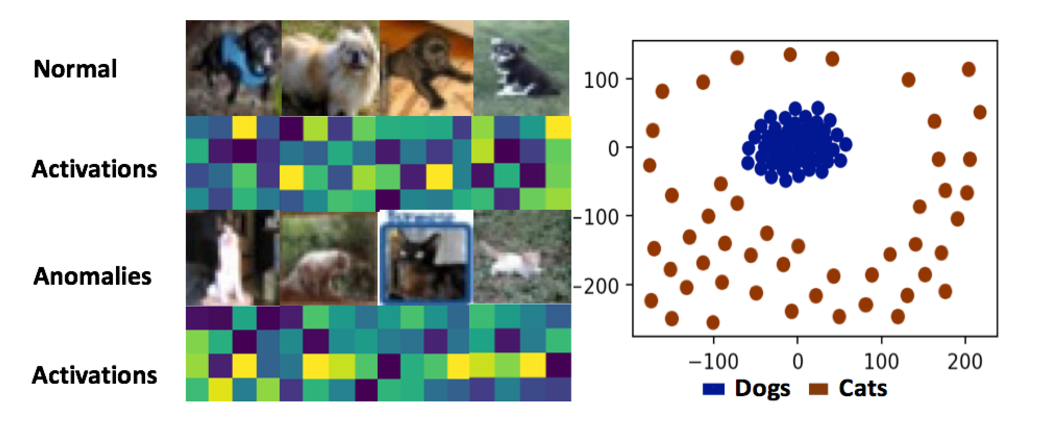
\includegraphics[width=0.8\textwidth]{images/activations}
%     \caption{Hidden layer (sigmoid) activations and its t-sne~\cite{tSNEVisualize2008} embeddings of OC-NN model for CIFAR-10 dataset.}
%     \label{fig:h_activations}
%     \vspace{-0.530cm}
% \end{figure}

We summarize our main contributions as follows:
\begin{itemize}
\item We derive a new one class neural network (OC-NN) model for anomaly detection. OC-NN uses a one class SVM like loss function to drive the training
of the neural network.
\item We propose an alternating minimization algorithm for learning the parameters of the OC-NN model. We observe that the subproblem of
the OC-NN objective is equivalent to a solving a quantile selection problem.
\item We carry out extensive experiments which convincingly demonstrate  that OC-NN  outperforms other state-of-the-art deep learning approaches
for anomaly detection on complex image and sequence data sets.
\end{itemize}

The rest of the paper is structured as follows. In Section~\ref{sec:background} we provide a detailed survey of related and relevant
work on anomaly detection. The main OC-NN model is developed in Section~\ref{sec:method}. The experiment setup, evaluation metrics and
model configurations are described in Section~\ref{sec:experiment-setup}. The results and analysis of the experiments are the focus of
Section~\ref{sec:experiment-results}. We conclude in Section~\ref{sec:conclusion} with a summary and directions for future work.


% !TEX root=../main.tex
\section{Related Work}
\label{ocnn:RelatedWork}
\begin{comment}
Consider a feature matrix $\X \in \Real^{N \times D}$,
where $N$ denotes the number of data points and $D$ the number of features for each point.
For example, $N$ could be the number of images in some photo collection, and $D$ the number of pixels used to represent each image.
The goal of anomaly detection is to determine which rows of $\X$ are anomalous, in the sense of being dissimilar to all other rows. We will use $\X_{n :}$ to denote the $n$th row of $\X$.
\end{comment}

%\subsection{A tour of anomaly detection methods}

Anomaly detection is a well-studied topic in Data Science~\cite{chandola2007outlier,charubook}. Unsupervised anomaly detection aims at discovering
rules to separate normal and anomalous data in the absence of labels. One-Class SVM (OC-SVM) is a popular unsupervised approach to detect anomalies, which constructs
a smooth boundary around the majority of probability mass of data~\cite{Scholkopf:2001}. OC-SVM will be  described in detail in Section~\ref{sec:ocsvm}.
In recent times, several approaches of feature selection and feature extraction methods have been proposed for complex, high-dimensional
data for use with OC-SVM ~\cite{cao2003comparison,neumann2005combined}.
Following the unprecedented success of using deep autoencoder networks, as feature extractors, in tasks as diverse as visual, speech anomaly detection~\cite{chong2017abnormal,marchi2017deep}, several hybrid models that combine feature extraction using deep learning and OC-SVM
have appeared~\cite{sohaib2017hybrid,erfani2016high}. The benefits of leveraging pre-trained transfer learning  representations for anomaly detection in hybrid models was made evident by the results obtained, using two publicly available~\footnote{Pretrained-models:http://www.vlfeat.org/matconvnet/pretrained/.} pre-trained CNN models: ImageNet-MatConvNet-VGG-F (VGG-F) and  ImageNet-MatConvNet-VGG-M (VGG-M)~\cite{andrews2016transfer}. However, these hybrid OC-SVM approaches are decoupled in the sense that the feature learning is task agnostic and not customized for anomaly detecion. Recently a deep model which trains a neural network by minimizing the volume of a hypersphere that encloses the network representations of the data is proposed ~\cite{pmlrv80ruff18a}, our approach differs from this approach by combining the ability of deep networks to extract progressively rich representation of data alongwith the one-class objective, which obtains the hyperplane to separate all the normal data points from the origin.
 %In this paper, we formulate and evaluate a new architecture for anomaly detection in complex, high-dimensional domains by integrating the one-class objective into neural network arhitecture. The proposed one-class neural network (OC-NN) model is trained using standard back-propogation algorithm to learn, rich differentiable features customized for anomaly detection. To the best of our knowledge, this is the first method proposed which
%combines the ability of deep networks to extract progressively rich representation of data
%with the one-class objective of creating a tight envelope around normal data to improve the performance
%for anomaly detection.

\begin{comment}
\subsection{Deep hybrid OC-SVM Models.}
A popular hybrid approach followed in unsupervised anomaly detection is to couple feature reduction and extraction methods alongwith SVMs~\cite{cao2003comparison,neumann2005combined,shen2008feature,widodo2007combination}. Several hybrid models have been proposed to leverage the representational power of deep learning to address scalability issues of SVMs~\cite{song2017hybrid,you2017hybrid,sohaib2017hybrid}. Deep learning architectures such as sparse stacked autoencoder (SAE)-based deep neural networks (DNNs)~\cite{sohaib2017hybrid}, deep belief networks (DBNs)~\cite{erfani2016high} are adopted for extracting robust features. DBNs are generative models consisting of multiple layers of latent variables ("hidden units"). The advantages of using DBNs are two-fold: (a) their ability to perform non-linear dimensionality reduction (b) learn high dimensional data representations. A DBN can be trained efficiently in a greedy layer-wise fashion by using a Restricted Boltzmann Machine (RBM)~\cite{hinton2010practical}. A Restricted Boltzmann machine model can be defined by joint energy function on the hidden variable $h_k$ with $K$ dimension and visible input variable $x_d$ with $D$ dimension as seen in Equation~\ref{energy}. The model parameters $W^P_{dk}$ encode the pairwise compatibility between $x_d$ and $h_k$ while the  parameters $W^B_k$ and $W^C_d$ are biases which, selectively activates either $h_k$ or $x_d$.

\begin{align}
\label{energy}
    E_W(\mbf{x},\mbf{h})&=
-\sum_{d=1}^D\sum_{k=1}^K W^P_{dk}x_dh_k - \sum_{k=1}^KW^B_k h_k - \sum_{d=1}^D W^C_d x_d
\end{align}

In the context of anomaly detection for images, the $\mbf{x}$ variables may represent (e.g  pixels of the image). The hidden units are binary vector of length $K$ less than original dimension of image $D$. Training an RBM implies finding the values of the parameters such that the energy is minimised. One possible approach is to maximise the log-likelihood of $x$ that is estimated by its gradient with respect to the model parameters using Contrastive Divergence (CD). The DBN consisting of stack of RBMs model encodes rich feature representations of the input within hidden units. While a hybrid model consisting of DBN, trained to extract generic underlying features, as inputs to one-class SVM trained are shown to be effective~\cite{erfani2016high}. The experiments in the aforementioned work were performed on real-datasets comprising 1D inputs, synthetic data or texture images, which have lower dimensionality and different data distribution compared to colour images or long protein sequences.
\end{comment}

%%%%%
\subsection{Robust Deep Autoencoders for anomaly detection}
Besides the hybrid approaches which use OC-SVM with deep learning features another approach for anomaly detection is to use deep autoencoders.
Inspired by RPCA~\cite{xu2010robust}, unsupervised anomaly detection techniques such as robust deep autoencoders can be used to separate
normal from anomalous data~\cite{zhou2017anomaly,chalapathy2017robust}.
Robust Deep Autoencoder (RDA) or Robust Deep Convolutional Autoencoder (RCAE) decompose input data $X$ into two parts $X = L_D + S$, where $L_D$ represents the latent representation the hidden layer of the autoencoder. The matrix  $S$ captures noise and outliers which are hard to reconstruct as shown in Equation~\ref{eqn:robust-ae}. The decomposition is carried out by optimizing the objective function shown in Equation~\ref{eqn:robust-ae}.

\begin{equation}
	\label{eqn:robust-ae}
	\min_{\theta, S} + ||L_D - D_{\theta}(E_{\theta}(L_D)) ||_{2}+ \lambda \cdot \| S^T \|_{2,1}
\end{equation}
 \hspace{1.8cm}   $s.t. \hspace{0.2cm} X - L_D -S = 0 $



The above optimization problem is solved using a combination of backpropagation and Alternating Direction Method of Multipliers (ADMM) approach~\cite{boyd2004convex}. In our experiments  we have carried out a detailed comparision between OC-NN and approaches based on robust autoencoders.

\begin{comment}
Notice that in the constraint of Equation~\ref{eqn:robust-ae} we split the input data X into two
parts, $L_D$ and $S$. $L_D$ is the input to an autoencoder $D_{\theta}(E_{\theta}(L_D))$ and
we train this autoencoder by minimizing the reconstruction error
 $||L_D - D_{\theta}(E_{\theta}(L_D)) ||_{2}$ through back-propagation. $S$, on the other
hand, contains noise and outliers which are learnt applying proximal methods following Alternating Direction Method of Multipliers (ADMM) ~\cite{boyd2004convex}. While $\lambda$ tuning parameter is selected in a semi-supervised fashion through grid-search for optimal $F1$ score.
RDA could be leveraged to detect anomalies similar to OC-SVM setting. The results obtained using our proposed approach of OC-NN are comparable to the results obtained on anomaly detection task on both MNIST and Cifar-10 datasets, as illustrated in Table~\ref{tbl:mnist-usps-anomaly-results-summary} and Table~\ref{tbl:cifar-10-pfam-anomaly-results-summary}.
\end{comment}

\subsection{One-Class SVM for anomaly detection}
\label{sec:ocsvm}

One-Class SVM (OC-SVM) is a widely used approach to discover anomalies in an unsupervised fashion~\cite{scholkopf2002support}. OC-SVMs are a special case of support vector machine, which learns a  hyperplane to separate all the data points from the origin in a reproducing kernel Hilbert space (RKHS) and maximises the distance from this hyperplane to the origin. Intuitively in OC-SVM all the data points are considered as positively labeled instances and the origin
as the only negative labeled instance. More specifically, given a training data $\X$, a set without any class information, and $\Phi(\X)$  a RKHS map function
from the input space to the feature space $F$,  a
hyper-plane or linear decision function $f(\X_{n :})$ in the feature space $F$ is constructed as
$f( \X_{n :} ) = w^T \Phi(\X_{n :}) - \bias$,  to separate as many as possible of the mapped vectors
${ \Phi(\X_{n :}), n: 1,2,...,N}$ from the origin. Here  $w$ is the norm perpendicular to the hyper-plane and $\bias$ is the bias of the hyper-plane. In order to
obtain $w$ and $\bias$, we need to solve the
following optimization problem,

\begin{equation}
\label{eqn:ocsvm-objective}
 \min_{w,\bias} \frac{1}{2} \| w \|_{2}^2+ \frac{1}{\nu} \cdot \frac{1}{N} \sum_{n = 1}^N \max( 0, \bias - \langle w, \Phi(\X_{n :}) \rangle ) - \bias.
\end{equation}

where $\nu \in (0,1)$, is a parameter that
controls a trade off between maximizing the distance of the
hyper-plane from the origin and the number of data points
that are allowed to cross the hyper-plane (the false positives).
%When $\nu$ is small, fewer data fall on the same side of the hyper-plane as the origin in the
%feature space $F$.




% % !TEX root=../main.tex
\section{The Proposed Approach}
\label{sec:ocnn_method}

We now present our one-class Neural Network (OC-NN) model for unsupervised anomaly detection.
The method can be seen as designing a neural architecture using an  OC-SVM equivalent loss function.
Using OC-NN we will be able to exploit and refine features obtained from unsupervised tranfer learning specifically for anomaly
detection. This in turn will it make it possible to discern anomalies in complex data sets where the decision boundary between normal and anomalous
is highly nonlinear.
\vspace{-0.1cm}
\subsection{One-Class Neural Networks (OC-NN)}
\label{sec:oc-nn}
We design a simple feed forward network with one hiden layer having linear or sigmoid activation $g(\cdot )$ and one output node. Generalizations to deeper
architectures is straightforward. The OC-NN objective can be formulated as:
\begin{equation}
	\label{eqn:oc-nn}
	\min_{w, V, \bias} \frac{1}{2} \| w \|_{2}^2 + \frac{1}{2} \| V \|_F^2 + \frac{1}{\nu} \cdot \frac{1}{N} \sum_{n= 1}^N \max( 0, \bias - \langle w, g( V  \X_{n :} ) \rangle ) - \bias
\end{equation}

where $w$ is the scalar output obtained from the hidden to output layer,
$V$ is the weight matrix from input to hidden units.
Thus the \underline{key insight} of the paper is to replace the dot product $\mathbf{\langle w,\Phi(\X_{n :}) \rangle}$ in OC-SVM with the dot product $\mathbf{\langle w,g(V\X_{n :})\rangle}$. This change will make it possible to leverage transfer learning features obtained using an autoencoder and create an additional layer to refine
the features for anomaly detection. However, the price for the change is that the objective becomes non-convex and thus the resulting algorithm
for inferring the parameters of the model will not lead to a global optima.

%which is randomly initialized from the uniform distribution within the range $[-1, 1]$.  $\nu \in (0,1)$, is the parameter that
%equates to the percentage of anomalies within data, found via grid search in the experiments. $\bias$ is the equivalent maximum margin separating plane from the origin.


%%%%
\begin{comment}
\subsection{Connection to OC-SVM}
\label{sec:connection_to_OC-SVM}

Clearly, Equation~\ref{eqn:oc-nn} is the special case of the Equation~\ref{eqn:ocsvm-objective} presented in the Section~\ref{sec:ocsvm}, where the weights $V$  in Equation~\ref{eqn:oc-nn} are randomly initialised, and not optimised, and $g$ is the either a $linear$ and $sigmoid$ activations.
More generally, for a deep network with parameters $w$, we have

\begin{equation}
\label{eqn:gen-oc-nn}
 \min_{w,\bias} \frac{1}{2} \| w \|_{2}^2 +\frac{1}{\nu} \cdot \frac{1}{N} \sum_{i = 1}^N \max( 0, \bias - \langle w, \Phi( \X_{n :} w ) \rangle ) - \bias
\end{equation}
\end{comment}

%%%%
\vspace{-0.1cm}
\subsection{Training the model}
\label{sec:training}
We can optimize Equation~\ref{eqn:oc-nn} using an alternate minimization approach: We first fix $r$ and optimize for $w$ and $V$. We then use
the new values of $w$ and $V$ to optimize $r$. However, as we  will show, the optimal value of $r$ is just the $\upsilon$-quantile of
the array $\langle w,g(Vx_{n})\rangle$. We first define the objective to solve for $w$ and $V$ as
% \vspace{-0.1cm}
\begin{equation}
                \label{eqn:minimize_w_V}
                 \underset{w, V}{\argmin} \frac{1}{2} \| w \|_{2}^2 + \frac{1}{2} \| V \|_F^2 + \frac{1}{\upsilon} \cdot \frac{1}{N} \sum_{n = 1}^N \ell( y_n, \hat{y}_n( w, V ) )
                 \end{equation}
                where
                \begin{align*}
                        \ell( y, \hat{y} ) &= \max( 0, y - \hat{y} ) \\
                        y_n       &= \bias \\
                        \hat{y}_n( w, V ) &= \langle w, g( V x_n ) \rangle
                \end{align*}

Similarly the optimization problem for $\bias$ is
\begin{equation}
\label{eqn:minimize_r}
\underset{\bias}{\argmin} \left( \frac{1}{N\upsilon} \cdot \sum_{n = 1}^N \max( 0, \bias - \hat{y}_n ) \right) - r
\end{equation}
\begin{comment}
%%%
\begin{enumerate}[(1)]
	\item Initialise $w^{(0)}, V^{(0)}, r^{(0)}$ randomly
	\item for $t = 1, 2, \ldots$
	\begin{enumerate}[(a)]
		\item find $(w^{(t+1)}, V^{(t+1)})$ that minimise the objective through Backpropagation (BP) algorithm.
		\begin{equation}
		\label{eqn:minimize_w_V}
		 \underset{w, V}{\argmin} \frac{1}{2} \| w \|_{2}^2 + \frac{1}{2} \| V \|_F^2 + \frac{1}{\upsilon} \cdot \frac{1}{N} \sum_{n = 1}^N \ell( y_n, \hat{y}_n( w, V ) )
		 \end{equation}
		where
		\begin{align*}
			\ell( y, \hat{y} ) &= \max( 0, y - \hat{y} ) \\
			y_n       &= \bias^{(t)} \\
			\hat{y}_n( w, V ) &= \langle w, g( V x_n ) \rangle
		\end{align*}

		\item pick $\bias^{(t)}$ to be the $\upsilon^{\text{th}}$ quantile of $\{ \hat{y}_n \}_{n = 1}^N$, where
		$$ \hat{y}_n^{(t+1)} = \langle w^{(t+1)}, g( V^{(t+1)} x_n ) \rangle. $$
	\end{enumerate}

\end{enumerate}

To justify step 2(b), let us observe that the optimisation with respect to $\bias$ is\\
%
\begin{equation}
\label{eqn:minimize_r}
\underset{\bias}{\argmin} \left( \frac{1}{N\upsilon} \cdot \sum_{n = 1}^N \max( 0, \bias - \hat{y}_n ) \right) - r
\end{equation}
\end{comment}
\begin{theorem}
Given $w$ and $V$ obtained from solving Equation~\ref{eqn:minimize_w_V}, the solution to Equation~\ref{eqn:minimize_r} is given
by the $\upsilon^{\text{th}}$ quantile of $\{ \hat{y}_n \}_{n = 1}^N$, where
                $$ \hat{y}_n = \langle w, g(V x_n ) \rangle. $$
\end{theorem}
\begin{proof}
 We can rewrite Equation~\ref{eqn:minimize_r} as:
\begin{align*}
%\underset{\bias}{\argmin} \left( \frac{1}{N\upsilon} \cdot \sum_{n = 1}^N \max( 0, \bias - \hat{y}_n ) \right) - r \\
\underset{\bias}{\argmin} \left( \frac{1}{N\upsilon} \cdot \sum_{n = 1}^N \max( 0, \bias - \hat{y}_n ) \right) - \left( \bias - \frac{1}{N} \sum_{n = 1}^{N} \hat{y}_n \right) \\
= \underset{\bias}{\argmin} \left( \frac{1}{N\upsilon} \cdot \sum_{n = 1}^N \max( 0, \bias - \hat{y}_n ) \right) - \left( \frac{1}{N} \sum_{n = 1}^{N} \left[ \bias - \hat{y}_n \right] \right) \\
= \underset{\bias}{\argmin} \left( \sum_{n = 1}^N \max( 0, \bias - \hat{y}_n ) \right) - \upsilon \cdot \left( \sum_{n = 1}^{N} \left[ \bias - \hat{y}_n \right] \right) \\
= \underset{\bias}{\argmin} \sum_{n = 1}^N \left[ \max( 0, \bias - \hat{y}_n ) - \upsilon \cdot \left( \bias - \hat{y}_n \right) \right] \\
= \underset{\bias}{\argmin} \sum_{n = 1}^N
\begin{cases} (1 - \upsilon) \cdot \left( \bias - \hat{y}_n \right) & \text{ if } \bias - \hat{y}_n > 0 \\ - \upsilon \cdot \left( \bias - \hat{y}_n \right) & \text{ otherwise}
\end{cases}
\end{align*}
% \vspace{0.4cm}
\vspace{-0.1cm}
We can observe that the derivative with respect to $r$ is
$$ F'( r ) = \sum_{n = 1}^N \begin{cases} (1 - \upsilon) & \text{ if } \bias - \hat{y}_n > 0 \\ -\upsilon & \text{ otherwise. } \end{cases} $$
Thus, by F'( r ) = 0 we obtain
%
\begin{align*}
	(1 - \upsilon) \cdot \sum_{n = 1}^N \indicator{ \bias - \hat{y}_n > 0 } &= \upsilon \cdot \sum_{n = 1}^N \indicator{ \bias - \hat{y}_n \leq 0 } \\
	&= \upsilon \cdot \sum_{n = 1}^N (1 - \indicator{ \bias - \hat{y}_n > 0 }) \\
	&= \upsilon \cdot N - \upsilon \cdot \sum_{n = 1}^N \indicator{ \bias - \hat{y}_n > 0 },
\end{align*}
or
\begin{equation}
 \frac{1}{N} \sum_{n = 1}^N \indicator{ \bias -\hat{y}_n > 0 }= \frac{1}{N} \sum_{n = 1}^N \indicator{ \hat{y}_n < r } = \upsilon
\end{equation}\\
This means we would require the $\nu^{\text{th}}$ quantile of $\{ \hat{y}_n \}_{n = 1}^N$.
\end{proof}
% \vspace{0.3cm}
%Algorithm
\vspace{-0.3cm}
\subsection{OC-NN Algorithm}
\label{sec:algorithm}
We summarize the solution in Algorithm~\ref{alg1}. We initialize $\bias^{(0)}$ in Line 2. We learn the parameters($w,V$) of the neural network
using the standard Backpropogation(BP) algorithm (Line 7). In the experiment section, we will train the model using features extracted from
an autoencoder instead of raw data points. However this has no impact on the OC-NN algorithm. As show  in Theorem 3.1, we solve for $\bias$
using the $\upsilon$-quantile of the scores $\langle y_{n} \rangle$. Once the convergence criterion is satisfied, the data points are
labeled normal or anomalous using the decision function $S_{n} = sgn(\hat{y}_{n} - r)$.

\begin{algorithm}
\caption{one-class neural network (OC-NN) algorithm}\label{alg:oc-nn}
\label{alg1}
\begin{algorithmic}[1]
\State{
\textbf{Input:} Set of points $\X_{n :},\hspace{0.2cm} n: 1,...,N$
}
\State{
\textbf{Output:} A Set of decision scores $S_{n :}=\hat{y}_{n :}$, n: 1,...,N for X
}

\State Initialise $\bias^{(0)}$
\State $t \gets 0$
\While{(no convergence achieved)}
\State Find $(w^{(t+1)}, V^{(t+1)})$ \Comment Optimize Equation~\ref{eqn:minimize_w_V} using BP.
\State $r^{t+1} \gets \nu^{\text{th}}$ quantile of $\{ \hat{y}_n^{t+1} \}_{n = 1}^N$
\State $t \gets t + 1$
\EndWhile \label{endwhile}
\State \textbf{end}
\State Compute decision score $S_{n :}=  \hat{y}_n -r  \mbox{ for each }  \X_{n :}$
\If{($S_{n :}$ $\geq$ 0)}
    \State $\X_{n :}$ is normal point
   \Else
    \State $\X_{n :}$ is anomalous
\EndIf

\State \textbf{return} $\{S_n\}$

\end{algorithmic}
\end{algorithm}
% \vspace{-0.05cm}
%
\noindent
{\bf Example:} We give a small example to illustrate that the minimum of the function
\[f(r) =  \left( \frac{1}{N\upsilon} \cdot \sum_{n = 1}^N \max( 0, \bias - y_n ) \right) - r\] occurs at the
the $\upsilon$-quantile of the set $\{y_{n}\}$. \\

Let $y =\{1,2,3,4,5,6,7,8,9\}$ and  $\upsilon = 0.33$. Then the minimum will occur at $f(3)$ as detailed in
the table below.
\[
\begin{array}{|r|l|r|}  \hline \hline
r & f(r) (\mbox{expr}) & f(r) (\mbox{value}) \\ \hline \hline
1 & \frac{1}{9*.33}[0 + 0 +\ldots 0] - 1 & -1.00 \\ \hline
2 & \frac{1}{9*.33}[1 + 0 +\ldots 0] - 2 & -1.67 \\ \hline
\rowcolor{green!20}
3 & \frac{1}{9*.33}[2 + 1 +\ldots 0] - 3 & -1.99  \\ \hline
4 & \frac{1}{9*.33}[3 + 2 + 1 +\ldots 0] - 4 & -1.98  \\ \hline
5 & \frac{1}{9*.33}[4 + 3 + 2 + 1\ldots 0] - 5 & -1.63  \\ \hline
6 & \frac{1}{9*.33}[5 + 4  + 3 + 2 + 1\ldots 0] - 6 & -0.94  \\ \hline
7 & \frac{1}{9*.33}[6 + 5  + 4 + 3 + 2 + 1\ldots 0] - 7 & 0.07  \\ \hline
8 & \frac{1}{9*.33}[7 + 6  + 5 + 4 + 3 + 2 + 1\ldots 0] - 8 & 1.43  \\ \hline
9 & \frac{1}{9*.33}[8 + 7  + 6 + 4 + \ldots 0] - 9 & 3.12  \\ \hline
\end{array}
\]


\begin{comment}
\subsection{Predicting with the model}

One convenient property of our model is that the anomaly detector will be inductive, i.e.\ it can generalise to unseen data points.
One can interpret the model as learning a non linear projection  of the input;
such a representation should thus be able to accurately model any unseen points that lie on the same manifold as the data used to train the model. Formally, $f( x ) = \langle w, \Phi( \X_{n :} w ) \rangle$  computes decision score of the given data point.
The "negative" or "closer" $\langle w, \Phi( \X_{n :} w ) \rangle$ is, to origin and the more likely the point is deemed to be anomalous.

%
\subsection{Relation to existing models}
Our contribution is breaking-new grounds, to integrate the OC-SVM equivalent objective into the neural
network architecture, utilizing the features extracted through unsupervised tranfer representation learning for anomaly detection.
Some previous works have employed deep networks for anomaly detection~\cite{chalapathy2017robust,zhou2017anomaly}. For example, the recent work of \cite{zhou2017anomaly} employed an autoencoder-inspired objective to train a robust deep autoencoder network, with extensions to capture structured noise within the data; Our method is distinct to robust deep autoencoders (RDA),  wherein we introduce a novel one-class neural network objective function illustrating the analytic derivation of $\nu^{th}$ quantile of the sorted output scores represents, the maximum margin distance,  separating normal data from anomalies. Although, nonlinear projections~\cite{bingham2001random,rathore2017ensemble} have been explored  for anomaly detection. We are unaware of prior usage of transfer learnt autoencoder networks integrated with one-class neural network objective to detect anomalies in unsupervised fashion.
\end{comment}

% !TEX root=../main.tex
\section{Experimental Setup}
\label{sec:ocnn_experiment-setup}

In this section, we show the empirical effectiveness of OC-NN formulation over the state-of-the-art methods on real-world data. Although our method is applicable in any context where autoencoders may be used for feature representation, e.g., speech.  Our primary focus will be on non-trivial high dimensional images.
%\vspace{-0.3 cm}
\subsection{Methods compared}
\label{sec:methods_compared}
We compare our proposed one-class neural networks (OC-NN) with the following state-of-the-art methods for anomaly detection:
\let\labelitemi\labelitemii
\begin{itemize}{}
	\item \textbf{OC-SVM -SVDD} as per formulation in ~\cite{scholkopf2002support}
    \item \textbf{Isolation Forest} as per formulation in ~\cite{liu2008isolation}.
	\item \textbf{Kernel Density Estimation (KDE)} as per formulation in ~\cite{parzen1962estimation}.
    \item \textbf{Deep Convolutional Autoencoder (DCAE)} as per formulation in ~\cite{masci2011stacked}.
    \item \textbf{AnoGAN} as per formulation in ~\cite{radford2015unsupervised}.
    \item \textbf{Soft-Bound and One Class Deep SVDD} as per formulation in ~\cite{pmlrv80ruff18a}.
    \item \textbf{Robust Convolutional Autoencoder (RCAE)} as per formulation in ~\cite{chalapathy2017robust}.
	\item \textbf{One-class neural networks (OC-NN) \footnote{\url{https://github.com/raghavchalapathy/oc-nn}}}, our proposed model as per Equation \ref{eqn:oc-nn}.
\end{itemize}
We used Keras~\cite{chollet2015keras} and  TensorFlow~\cite{abadi2016tensorflow} for the implementation of OC-NN, DCAE, RCAE \footnote{\url{https://github.com/raghavchalapathy/rcae}}
For OC-SVM\footnote{\url{http://scikit-learn.org/stable/auto_examples/svm/plot_oneclass.html}} and Isolation Forest\footnote{\url{http://scikit-learn.org/stable/modules/generated/sklearn.ensemble.IsolationForest.html}}, we used publicly available implementations.

\begin{table}[!t]
    \centering
    \renewcommand{\arraystretch}{1.25}
    \setlength{\tabcolsep}{6pt}
    %\scalebox{0.85}{
    \begin{tabular}{@{}llll@{}}
        \toprule
        \toprule
        Dataset & \# instances & \# anomalies & \# features \\
        \toprule
        {\tt Synthetic}       & 190   & 10                                        & 512 \\
        {\tt MNIST}           & single class   & 1\%  ( from all class)            & 784 \\
        {\tt CIFAR$-$10}      & single class    & 10\% ( from all class)           &3072 \\
        {\tt GTSRB }           & 1050 (stop signs )     & 100 (boundary attack)  &3072 \\
        \bottomrule
    \end{tabular}
    %}
    %\vspace{0.1 cm}
    \caption{Summary of datasets used in experiments.}
    \label{tbl:datasets}
    \vspace{-\baselineskip}
\end{table}

% \vspace{-0.5 cm}
\subsection{Datasets}
%%\vspace{-0.2 cm}
We compare all methods on synthetic and four real-world datasets as summarized below :
\begin{itemize}
	\item {\tt Synthetic Data}, consisting of 190 normal data points 10 anomalous points drawn from normal distribution with dimension $512$.
	\item {\tt MNIST}, consisting of 60000 $28\times28$ grayscale images of handwritten digits  in 10 classes, with 10000  test images~\cite{lecun2010mnist}.
	\item {\tt GTSRB }, are $32\times32$ colour images comprising of  adversarial boundary attack on stop signs boards~\cite{stallkamp2011german}.
	\item {\tt CIFAR$-$10} consisting of 60000 $32\times32$ colour images in 10 classes, with 6000 images per class~\cite{krizhevsky2009learning}.
\end{itemize}

For each dataset, we perform further processing to create a well-posed anomaly detection task, as described in the next section.
\vspace{-0.3 cm}

\subsection{Evaluation of Models}
\label{sec:evaluationOfModels}
% Shallow methods compared
\subsubsection{\textbf{Baseline Model Parameters:}}
\label{sec:baselinemodel_parameters.}
The proposed OC-NN method is compared with several state-of-the-art baseline models as illustrated in Table~\ref{tab:ocnn_results}. The model parameters of shallow baseline methods are used as per implementation in~\cite{pmlrv80ruff18a}. Shallow Baselines (i) Kernel OC-SVM/SVDD with
Gaussian kernel. We select the inverse length scale $\gamma$ from
$\gamma$  $\in$ {$2^{ - 10}$ , $2^{ - 9}$, . . . , $2^{ - 1}$ via grid search using the performance on a small holdout set (10) \% of randomly drawn test samples). We run all experiments for $\nu = 0.1$ and report the better result. (ii) Kernel density estimation (KDE). We select the bandwidth \textit{h} of the Gaussian kernel from \textit{h} $ \in {2^{0.5} , 2 ^1, . . . , 2^5}$ via 5-fold cross-validation using  the log-likelihood score. (iii) For the  Isolation Forest (IF) we set the number of trees to \textit{t} = 100 and the sub-sampling size to $\Psi = 256$, as recommended in the original work~\cite{pmlrv80ruff18a}.
\vspace{-0.4cm}
% Deep Anomaly detection models compared
\subsubsection{ \textbf{Deep Baseline Models:}}
We compare OC$-$NN models to  four deep approaches described Section ~\ref{sec:methods_compared}.
We choose to train DCAE using the Mean sqaure error (MSE) loss since our experiments are on image data. For the DCAE encoder, we employ the same network architectures as we use for Deep SVDD, RCAE, and OC-NN models. The decoder is then constructed symmetrically, where we substitute max-pooling with upsampling. For AnoGAN we follow the implementation as per ~\cite{radford2015unsupervised} and set
the latent space dimensionality to $256$.
For we Deep SVDD, follow the implementation as per ~\cite{pmlrv80ruff18a} and employ a  two phase learning rate schedule (searching + fine tuning) with initial learning rate $\eta$ = $10^{ - 4}$  and subsequently $\eta$ = $10^{ - 5}$. For DCAE we train 250 + 100 epochs, for Deep SVDD 150 + 100. Leaky ReLU activations are used with leakiness $\alpha=0.1$. For RCAE we train the autoencoder using the robust loss and follow the parameter settings as per formulation in ~\cite{chalapathy2017robust}.

%OC-NN Model Architecture proposed
\subsubsection{ \textbf{One-class neural Networks (OC-NN):}}
\label{model_architecture}
In OC-NN technique firstly, a deep autoencoder is trained to obtain the representative features of the input as illustrated in Figure~\ref{fig:model-architecture}(a). Then, the encoder layers of this pre-trained autoencoder is copied and fed as input to the feed-forward network with one hidden layer as shown in Figure~\ref{fig:model-architecture}(b). The summary of feed forward network architecture's used for various datasets is presented in Table~\ref{tbl:feed-forward-OC-NN}. The weights of encoder network are not frozen (but trained) while we learn feed-forward network weights, following the algorithm summarized in Section~\ref{sec:algorithm}. A feed-forward neural network consisting of single hidden layer, with  linear activation functions produced the best results, as per Equation~\ref{eqn:oc-nn}.  The optimal value of parameter $\nu$ $\in$ ${[0, 1]}$ which is equivalent to the percentage of anomalies for each data set, is set according to respective outlier proportions.

% \vspace{-0.2cm}
% Model architectures tested
% \begin{figure*}
% \subfloat[Autoencoder .\label{sfig:autoencoder-for-representation-learning}]{%
%   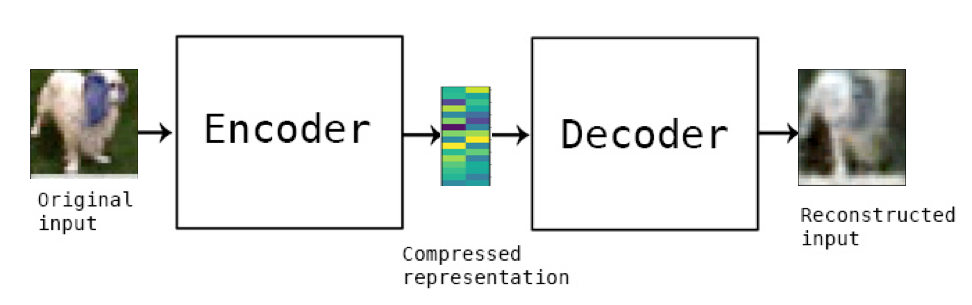
\includegraphics[width=.40\linewidth]{images/transferLearningAE}%
% }\hspace{0.5cm}
% \subfloat[one-class neural networks. \label{sfig:oc-nn-model-architecture}]{%
%   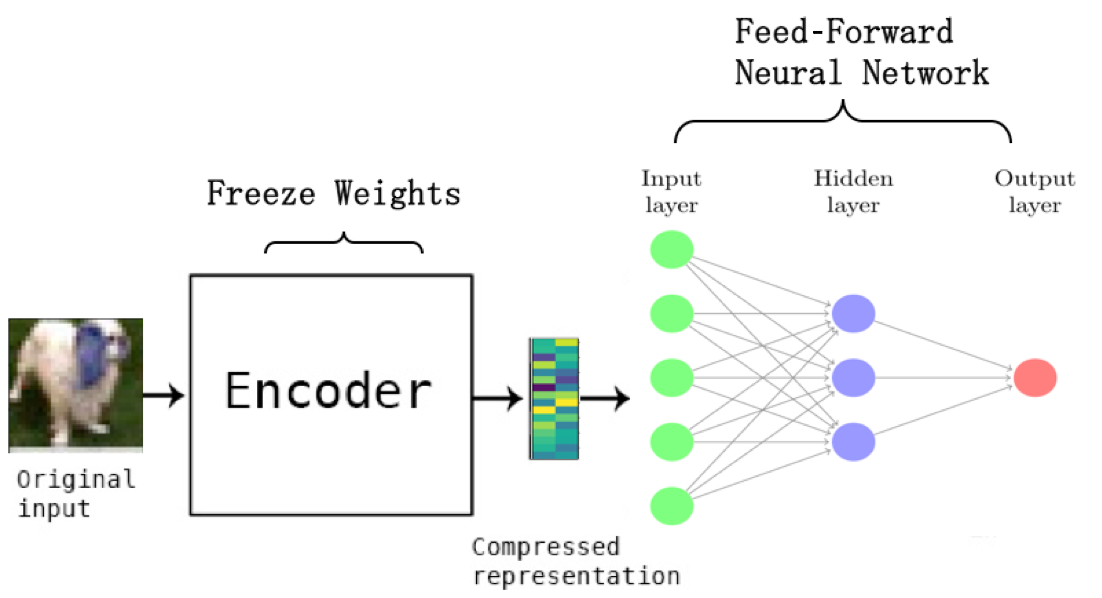
\includegraphics[width=.40\linewidth]{images/oneClassNN_model}%
% }
% \caption{Model architecture of Autoencoder  and the proposed one-class neural networks (OC-NN).}
% \label{fig:model-architecture}
% \end{figure*}
% %  End of the Figure

\begin{figure}[!t]
     \begin{subfigure}[b]{1\textwidth}
   \centering
   {\includegraphics[scale=0.50]%{catswithrotatedcats}}
{images/transferLearningAE}}
\caption{Autoencoder.}
        \end{subfigure}%
        \hfill
        \vspace{2mm}
     \begin{subfigure}[b]{1\textwidth}
\centering
   {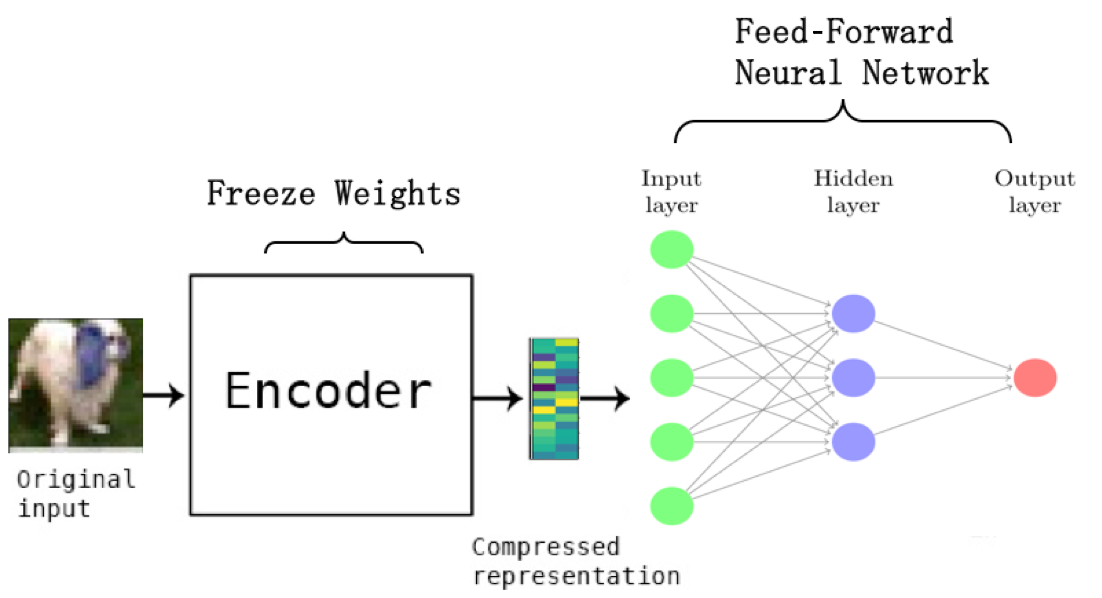
\includegraphics[scale=0.50]{images/oneClassNN_model}}
 \caption{One-class neural networks.}
        \end{subfigure}%
    \caption{
     Model architecture of Autoencoder  and the proposed one-class neural networks (OC-NN).
    }
    \label{fig:model-architecture}
\end{figure}




%Table containing the feed forward network architectures used in experiments
\begin{table}[!t]
    \centering
    \renewcommand{\arraystretch}{1.25}
    \setlength{\tabcolsep}{6pt}
    %\scalebox{0.85}{
    \begin{tabular}{@{}llll@{}}
        \toprule
        \toprule
         Dataset& \#    Input (features) & \# hidden layer( or output) \# optional layer  \\
        \toprule
        {\tt Synthetic }      & 512     & 128   & 1 \\
        {\tt MNIST}           & 32      & 32    & None \\
        {\tt CIFAR$-$10}      & 128     & 32    & None \\
        {\tt GTSRB }          & 128     & 32    & 16 \\
        \bottomrule
    \end{tabular}
    %}
    %\vspace{0.1 cm}
    \caption{Summary of best performing feed-forward network architecture's used in OC-NN model for experiments.}
    \label{tbl:feed-forward-OC-NN}
    \vspace{-\baselineskip}
\end{table}
% end of the table


































\section{Experimental Results}
\label{sec:ocnn_experiment-results}

In this section, we present empirical results produced by OC-NN model on synthetic and real data sets. We perform a comprehensive set of experiments to demonstrate that on complex data sets OC-NN performs on par with state-of-the-art methods and outperformed conventional shallow methods in some scenarios.
%%%%% Synthetic Dataset
\subsection{\tt OC-NN for Synthetic Data}
Single cluster consisting of 190 data points using $\mu=0$ and $\sigma = 2$ are generated as normal points , along with 10 anomalous points drawn from normal distribution with $\mu=0$ and $\sigma = 10$ having  dimension $d=512$. Intuitively, the latter normally distributed points are treated as being anomalous, as the corresponding points have different distribution characteristics to the majority of the training data. Each data point is flattened as a row vector, yielding a 190 $\times$ 512 training matrix and 10 $\times$ 512 testing matrix. We use a simple feed-forward neural network model with one-class neural network  objective as per Equation~\ref{eqn:oc-nn}.\\
%using network parameter settings described in Section~\ref{sec:feed forward oc-nn-model-config}.\\
\textbf{Results}.
From Figure~\ref{fig:synthetic-histogram}, we see that it is a near certainty for all $10$ anomalous points, are accurately identified as outliers with decision scores being negative for anomalies. It is evident that, the OC-NN formulation performs on par with classical OC-SVM in detecting the anomalous data points. In the next sections we apply to image and sequential data and demonstrate its effectiveness.


%% Results for Synthetic dataset
\begin{figure}
    \centering
    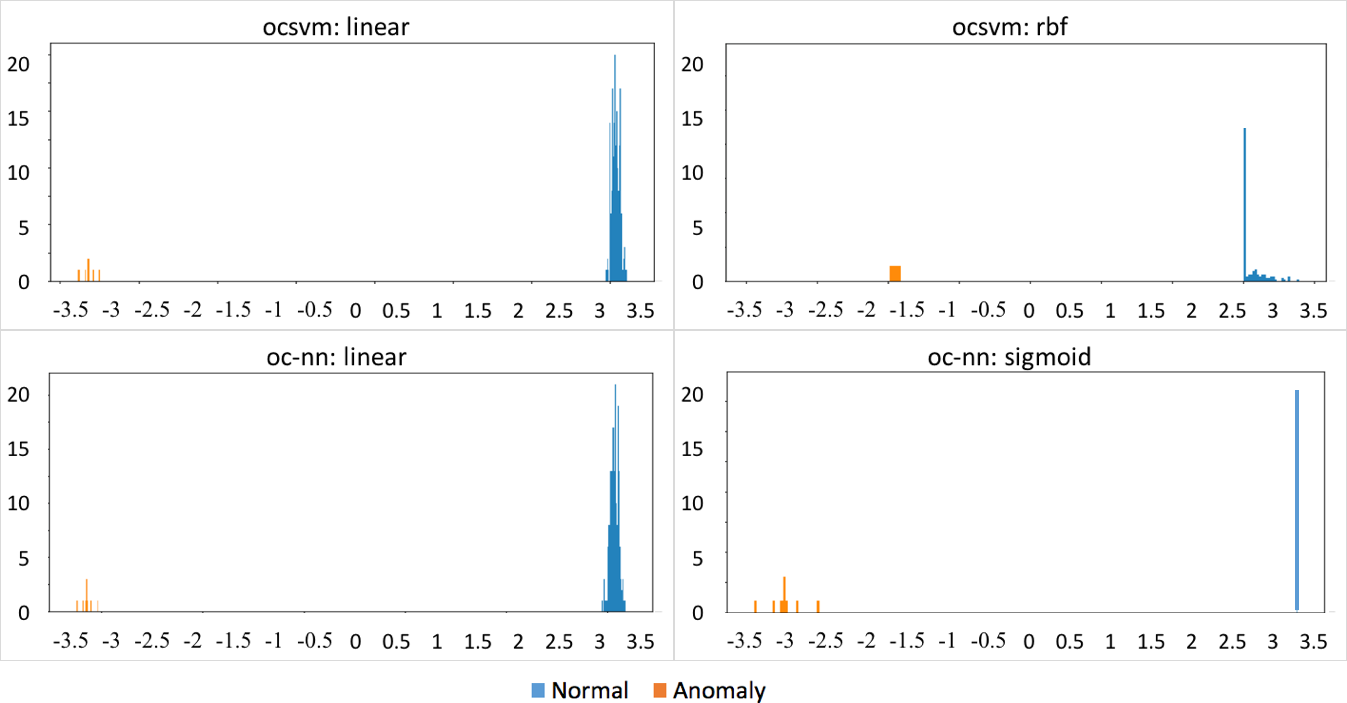
\includegraphics[scale=0.38]{images/s1.png}
    \caption{Decision Score Histogram of anomalous vs normal data points, {\tt synthetic} dataset.}
    \label{fig:synthetic-histogram}
\end{figure}


% Results for Most anomalous and most normal images detected for MNIST dataset
\begin{figure*}
\subfloat[Normal samples detected.  \label{sfig:normalmnistRcae}]{%
  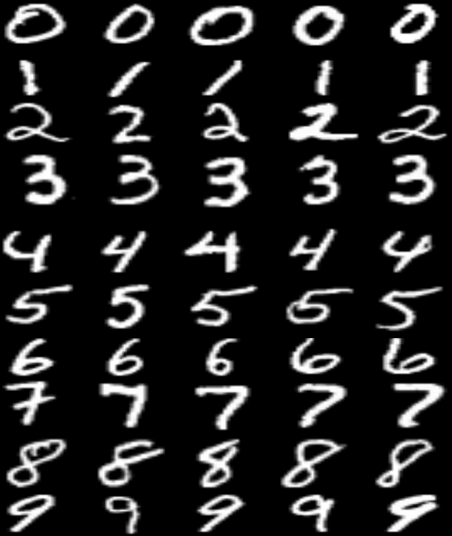
\includegraphics[width=.30\linewidth]{images/mnistNormalRCAE}%
}\hspace{0.5cm}
\subfloat[In-class anomalous samples. \label{sfig:mnistAnomalyRCAE}]{%
  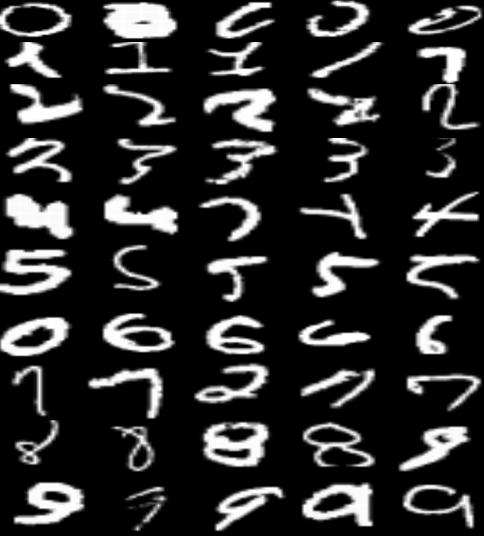
\includegraphics[width=.32\linewidth]{images/mnistAnomalyRCAE}%
}
\caption{MNIST Most normal and in-class anomalous MNIST digits detected by RCAE. }
\label{fig:mnistRCAEresults}
\end{figure*}
%  End of the Figure


% Results for Most anomalous and most normal images detected for MNIST dataset
\begin{figure*}
\subfloat[Normal samples. \label{sfig:mnistnormalOCNN}]{%
  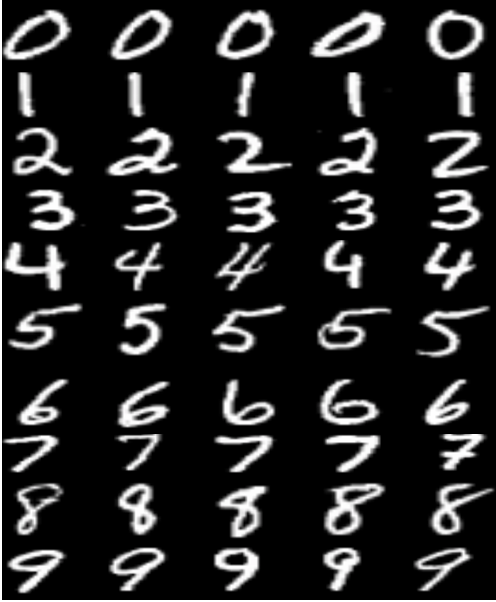
\includegraphics[width=.30\linewidth]{images/mnistnormalOCNN}%
}\hspace{0.5cm}
\subfloat[In-class anomalous samples. \label{sfig:mnistOutlierOCNN}]{%
  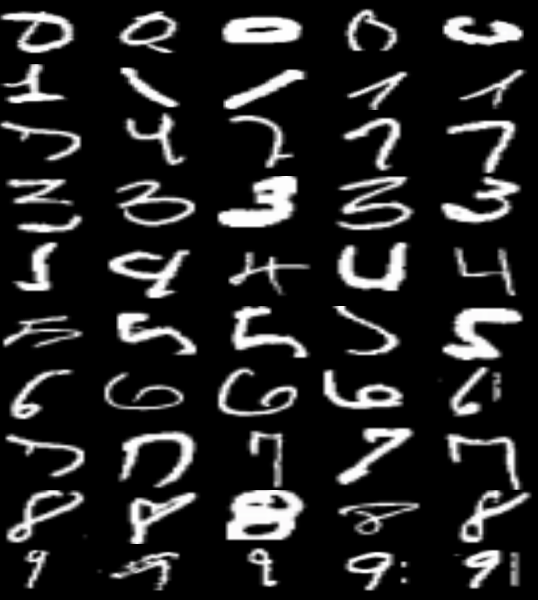
\includegraphics[width=.325\linewidth]{images/mnistOutlierOCNN}%
}
\caption{MNIST Most normal and in-class anomalous MNIST digits detected by OC-NN.}
\label{fig:mnistOCNNresults}
\end{figure*}
%  End of the Figure


%%%%% Mnist Dataset
\subsection{\tt OC-NN on MNIST and CIFAR-10}
\textbf{Setup}
Both MNIST and CIFAR-10  have ten different classes from which we construct one-class classification dataset.  One of the classes is the normal class and
samples from the remaining classes represent anomalies. We use the original training and test splits in our
experiments and only train with training set examples from
the respective normal class. This produces normal instances set of sizes
of n $\approx$ 6000 for MNIST and n $\approx$ 5000 for CIFAR-10 respectively.
Both MNIST and CIFAR-10 test sets have $10000$ samples per class.
The training set comprises of normal instances for each class along with anomalies sampled from
all the other nine classes. The number of anomalies used within training set consists of 1\% normal class for MNIST and  10\% of normal class for CIFAR-10 dataset respectively. We pre-process all images with global contrast normalization using the $L1$
norm and finally rescale to [0, 1] via min-max-scaling.\\
\textbf{Network architectures} For both MNIST and CIFAR-10 datasets, we employ LeNet type
CNNs, wherein each convolutional module consists of a convolutional layer followed by leaky ReLU activations and $2 \times 2$ max-pooling. On MNIST, we use a CNN with two modules, $8\times(5\times5\times1)$-filters followed by $4\times(5\times5\times1)$-filters, and a final dense layer of 32 units. On CIFAR-10,
we use a CNN with three modules, $32 \times (5 \times 5 \times3)$-filters,
$64\times(5\times5\times3)$-filters, and $128\times(5\times5\times3)$-filters, followed
by a final dense layer of $128$ units. We use a batch size of
$200$ and set the weight decay hyperparameter to $ \lambda= 10^{ - 5}$.\\
{\textbf{Results:}}
Results are presented in Table ~\ref{tab:ocnn_results}. RCAE
clearly outperforms both its shallow and deep competitors
on MNIST. On CIFAR-10 the results are convincing but for certain classes the shallow baseline methods outperform the deep models. OC-NN, Soft and One-class Deep SVDD however, shows an overall robust performance. On CIFAR-10 classes such as $AUTOMOBILE$, $BIRD$ and $DEER$ which have less global contrast, as illustrated in Table~\ref{tab:ocnn_results} (indicated in blue color)  OC-NN seems to outperform the shallow methods, Soft and One-class Deep SVDD methods, this is indicative of their future potential on similar data instances.  It is interesting to note that shallow OCSVM/SVDD and KDE perform better than deep methods on two of the ten CIFAR-10 classes. We can see that normal examples of the classes  such as $FROG$ and $TRUCK$ on which OCSVM/SVDD performs best as illustrated in Figure~\ref{fig:ocsvmresults} seem to have strong global structures. For example, TRUCK images are mostly divided horizontally into street and sky, and  $FROG$ have similar colors globally. For these classes,  the performance significantly depends on choice of network architecture. Notably, the One-Class Deep SVDD performs slightly better than its soft-boundary counterpart on both datasets. Figure ~\ref{fig:mnistRCAEresults}, Figure ~\ref{fig:mnistOCNNresults} and Figure ~\ref{fig:cifar10_rcae_results} , Figure ~\ref{fig:cifar10_ocnn_results} show examples of the most normal and most anomalous in-class samples detected by RCAE and OC-NN for MNIST and CIFAR-10 dataset respectively.

% Results for Most anomalous and most normal images detected for CIFAR10 dataset
\begin{figure*}
\subfloat[Normal samples.  \label{sfig:cifar10NormalRCAE}]{%
  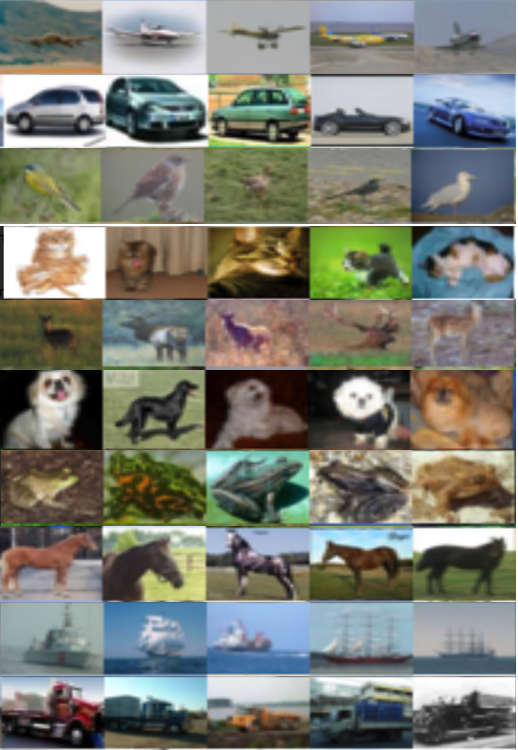
\includegraphics[width=.29\linewidth]{images/cifar10NormalRCAE}%
}\hspace{0.5cm}
\subfloat[In-class anomalous samples. \label{sfig:cifar10AnomalyRCAE}]{%
  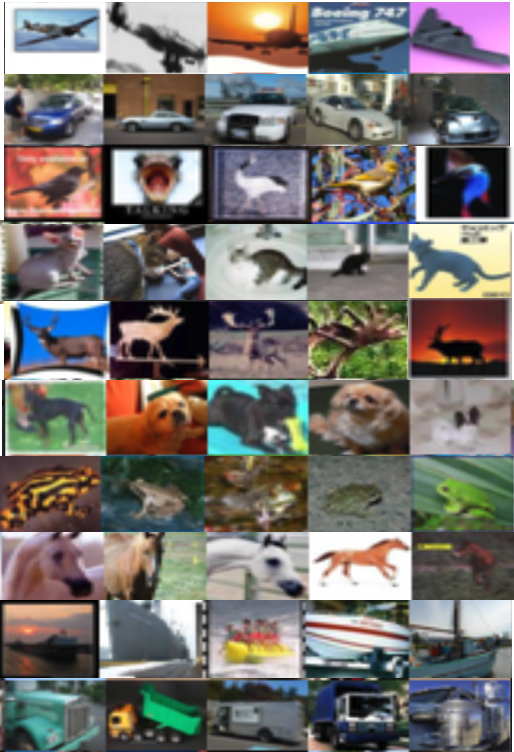
\includegraphics[width=.29\linewidth]{images/cifar10AnomalyRCAE}%
}
\caption{CIFAR-10 Most normal and in-class anomalous CIFAR10 digits detected by RCAE. }
\label{fig:cifar10_rcae_results}
\end{figure*}
%  End of the Figure


% Results for Most anomalous and most normal images detected for CIFAR10 dataset
\begin{figure*}
\subfloat[Normal samples . \label{sfig:cifar10normalOCNN}]{%
  \includegraphics[width=.29\linewidth]{images/cifar10normalOCNN}%
}\hspace{0.5cm}
\subfloat[In-class anomalous samples. \label{sfig:cifar10OutlierOCNN}]{%
  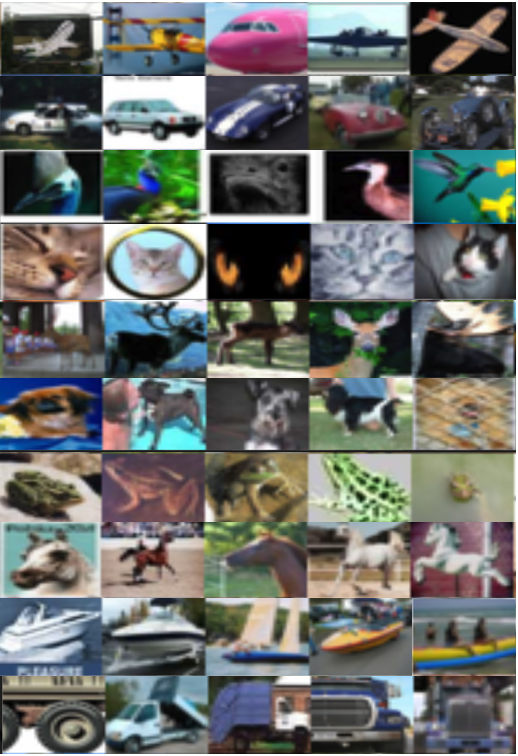
\includegraphics[width=.29\linewidth]{images/cifar10OutlierOCNN}%
}
\caption{CIFAR-10 Most normal and in-class anomalous CIFAR10 digits detected by OC-NN.}
\label{fig:cifar10_ocnn_results}
\end{figure*}
%  End of the Figure

% Results for Most anomalous and most normal images detected for CIFAR10 dataset for
\begin{figure*}
\subfloat[Normal samples . \label{sfig:cifar10normalOCSVM}]{%
  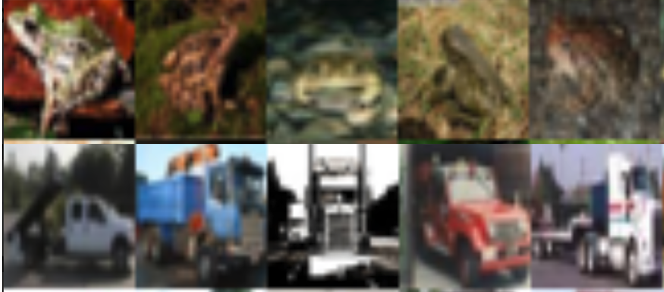
\includegraphics[width=.31\linewidth]{images/cifar10normalOCSVM}%
}\hspace{0.5cm}
\subfloat[In-class anomalous samples. \label{sfig:cifar10OutlierOCSVM}]{%
  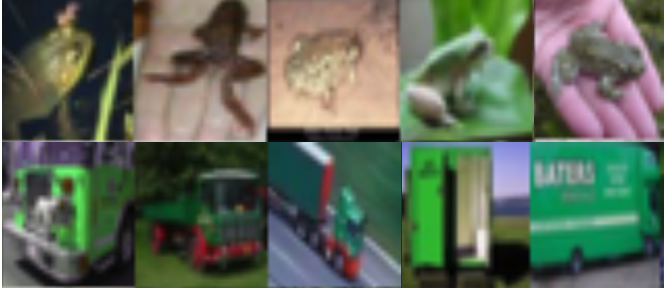
\includegraphics[width=.31\linewidth]{images/cifar10OutlierOCSVM}%
}
\caption{Most normal (left) and most anomalous (right) in-class
examples determined by OCSVM-SVDD for in which OCSVM-SVDD performs best.}
\label{fig:ocsvmresults}
\end{figure*}
%  End of the Figure




\subsection{\tt  Detecting Adversarial attacks on GTSRB stop signs using OC-NN }
\textbf{Setup:}
In many applications (eg. autonomous driving) it is of paramount interest to effectively detect the adversarial samples to ensure safety and security. In this experiment, we
examine  the performance of proposed algorithms on  detecting
adversarial examples. We consider the “stop sign”
class of the German Traffic Sign Recognition Benchmark
(GTSRB) dataset, for which we generate adversarial examples
from randomly drawn stop sign images of the test set
using Boundary Attack~\cite{brendel2017decision}. We create training dataset consists of n = 1150 examples obtained by combining the normal and anomalous samples in both train and test samples. The  number of normal instances n = 1050 stop signs ( 780  from train set +  270 test set ) alongwith  100
adversarial examples are added to obtain training set. We pre-process the
data by removing the 10\% border around each sign, and then resize every image to $32 \times 32$ pixels following the same setup as in ~\cite{pmlrv80ruff18a}. Furthermore, we  apply global contrast normalization using the $L1-norm$ and rescale to the unit interval $[0, 1]$.\\
\textbf{Network architecture} We use a CNN with LeNet architecture having three convolutional modules, $16\times(5\times5\times3)$-filters, $32 \times (5 \times 5 \times 3)$-filters, and $64 \times (5 \times 5 \times 3)$-filters, followed by a final dense layer of 32 units. We train with a smaller batch size of 64, due to the dataset size and set again hyperparamter $\lambda = 10^{ - 6}$.\\
\textbf{Results:}
Results Table ~\ref{tab:gtsrbresults} illustrates the AUC scores obtained. The RCAE outperforms all the other deep models. Figure ~\ref{fig:gtsrbrcaeresults} and Figure ~\ref{fig:gtsrbocnnresults}  shows the most anomalous samples detected by RCAE and OCNN methods respectively, the outliers in this experiment are the images in odd perspectives and the ones that are cropped incorrectly.

\begin{table*}[!t]
   \caption{Average AUCs in \% with StdDevs (over 10 seeds) per method on MNIST and CIFAR-10 dataset.}
   \label{tab:ocnn_results}
   \small % text size of table content
   \centering % center the table
   \begin{tabular}{lccccccccr} % alignment of each column data
   \toprule[\heavyrulewidth]\toprule[\heavyrulewidth]
   \textsc{\pbox{20cm}{Normal \\ Class}} & \textsc{\pbox{20cm}{OCSVM / \\ SVDD}} & \textsc{KDE} &  \textsc{IF} & \textsc{DCAE} & \textsc{ANOGAN} & \textsc{\pbox{20cm}{SOFT-BOUND \\ DEEP SVDD}} & \textsc{\pbox{20cm}{ONE-CLASS \\ DEEP SVDD}} & \textsc{OC-NN} & \textsc{RCAE} \\
   \midrule
   0 & 96.75±0.5 & 97.1±0.0 & 95.32±1.2  & 99.90±0.0 & 96.6±1.3 & 98.66±1.3     & 97.78±0.0 & 97.60±1.7 &
   \bf{99.92±0.0}\\
   1 & 99.15±0.4 & 98.9±0.0 & 99.35±0.0  & 99.96±2.1 & 99.2±0.6 & 99.15±0.0     & 99.08±0.0 & \color[rgb]{0,0,1}99.53±0.0 & \bf{99.97±2.2}\\
   2 & 79.34±2.2 & 79.0±0.0 & 73.15±4.5  & 96.64±1.3 & 85.0±2.9 & 88.09±2.2     & 88.74±1.2 & 87.32±2.1 & \bf{98.01±1.2}\\
   3 & 85.88±1.3 & 86.2±0.0 & 81.34±2.8 & 98.42±0.0 &  88.7±2.1 &  88.93±3.4     & 88.26±3.2 & 86.52±3.9 & \bf{99.25±0.0}\\
   4 & 94.18±1.5 & 87.9±0.0 & 87.40±2.6  & 98.72±0.0 & 89.4±1.3 & 93.88±2.3     & 95.24±1.4 & 93.25±2.4 & \bf{99.23±0.0}\\
   5 & 72.77±3.7 & 73.8±0.0 & 73.96±2.9  & 97.80±1.3 & 88.3±2.9 & 84.35±3.1     & 83.76±3.1 & \color[rgb]{0,0,1}86.48±3.3 & \bf{99.21±0.0}\\
   6 & 95.14±1.1 & 87.6±0.0 & 88.65±0.0  & 99.74±0.0 & 94.7±2.7 & 97.74±0.0     & 97.99±0.0 & 97.12±1.4 & \bf{99.81±1.1}\\
   7 & 91.86±1.6 & 91.4±0.0 & 91.44±1.8  & 99.08±2.2 & 93.5±1.8 & 92.60±1.2     & 93.55±2.3 & 93.64±2.1 & \bf{99.18±0.0}\\
   8 & 88.65±1.2 & 79.2±0.0 & 75.10±3.7  & 96.98±0.0 & 84.9±2.1 & 90.69±3.3     & 90.25±3.1 & 88.54±4.7 & \bf{98.50±2.2}\\
   9 & 92.53±1.9 & 88.2±0.0 & 87.59±1.5  & 98.04±1.3 & 92.4±1.1 & 94.28±2.5     & 94.12±2.4 & 93.54±3.3 & \bf{98.98±1.3}\\
   \hline
  \textsc{Aeroplane}    & 60.37±1.3 & 61.2±0.0 & 63.99±1.1  &71.21±1.5& 67.1±2.5 & 66.15±1.1 & 67.33±2.2 & 60.42±1.9  & \bf{72.04±2.5}\\
   \textsc{Automobile}  & 63.03±1.4 & 63.0±0.0 & 60.56±1.0  &63.05±2.3& 54.7±3.4 & 57.64±3.2 & 58.14±3.1 & \color[rgb]{0,0,1}61.97±2.0  & \bf{63.08±2.1}\\
   \textsc{Bird}        & 63.47±1.0 & 50.1±0.0 & 64.51±1.1  &71.50±1.1& 52.9±3.0 & 61.99±1.4 & 61.35±1.5 & \color[rgb]{0,0,1} {63.66±1.4} & \bf{71.67±1.3}\\
   \textsc{Cat}         & 60.25±0.9 & 56.4±0.0 & 56.16±2.6  &60.57±0.0& 54.5±1.9 & 57.56±4.1 & 55.72±1.4 & 53.57±2.1  & \bf{60.63±1.1}\\
  \textsc{Deer}         & 69.15±0.8 & 66.2±0.0 & 72.66±1.1  &70.85±2.2& 65.1±3.2 & 63.36±1.3 & 63.32±1.2 & \color[rgb]{0,0,1}67.40±1.7  & \bf{72.75±3.3}\\
   \textsc{Dog}         & 66.24±1.5 & 62.4±0.0 & 61.46±2.7  &62.74±2.1& 60.3±2.6 & 58.58±1.2 & 58.68±1.4 & 56.11±2.1  & \bf{63.96±3.3}\\
   \textsc{Frog}        & \bf{71.57±1.5} & {71.3±0.0} & 68.06±2.1  &65.17±4.1& 58.5±1.4 & 63.93±3.1 & 64.45±2.1 & 63.31±3.0  & {64.88±4.2}\\
   \textsc{Horse}       & 63.38±0.8 & 62.6±0.0 & 63.04±1.5  &61.11±1.4& 62.5±0.8 & 60.20±2.2 & 59.80±2.6 & 60.09±2.7  &
   \bf{63.64±0.0}\\
  \textsc{Ship}         & 60.44±1.1 & {65.1±0.0} & 68.01±1.3  &74.18±1.2& 74.68±4.1 & 70.21±1.1 & 67.44±2.2 & 64.67±1.6  & \bf{74.72±1.1}\\
  \textsc{Truck}        & \bf{75.81±0.8} & {74.0±0.0} & 72.83±1.1  &71.36±4.3& 66.5±2.8 & 72.91±3.3 & 68.03±3.2 & 60.32±4.9  & {74.47±1.5}\\
   \bottomrule[\heavyrulewidth]
   \end{tabular}
\end{table*}


% begin of table
\begin{table}[ht]
\caption{Average AUCs in \% with StdDevs (over 10 seeds) per
method on GTSRB stop signs with adversarial attacks.} % title of Table
\centering % used for centering table
\begin{tabular}{l l } % centered columns (4 columns)
\hline\hline %inserts double horizontal lines
\bf{\textsc{Method}} & \bf{\textsc{AUC}}\\ [0.5ex] % inserts table
%heading
\hline % inserts single horizontal line
OC-SVM/SVDD & 52.5 ± 1.3 \\ % inserting body of the table
KDE & 51.5 ± 1.6 \\
IF & 53.37±2.9 \\
AnoGAN & - \\
DCAE & 79.1±3.0 \\
SOFT-BOUND. DEEP SVDD & 67.53±4.7 \\
ONE-CLASS. DEEP SVDD & 67.08±4.7 \\
OC-NN & 63.53±2.5 \\
\bf{\bf{RCAE $\lambda =0$}} &\bf{87.45±3.1} \\
\bf{RCAE} & {$\bf{87.39 \pm 2.7}$} \\ [1ex] % [1ex] adds vertical space
\hline %inserts single line
\end{tabular}
\label{tab:gtsrbresults}
\end{table}
% end of table



% Results for Most anomalous and most normal images detected for GTSRB dataset
\begin{figure*}
\subfloat[Top 50 normal samples.  \label{sfig:normalGtsrb}]{%
  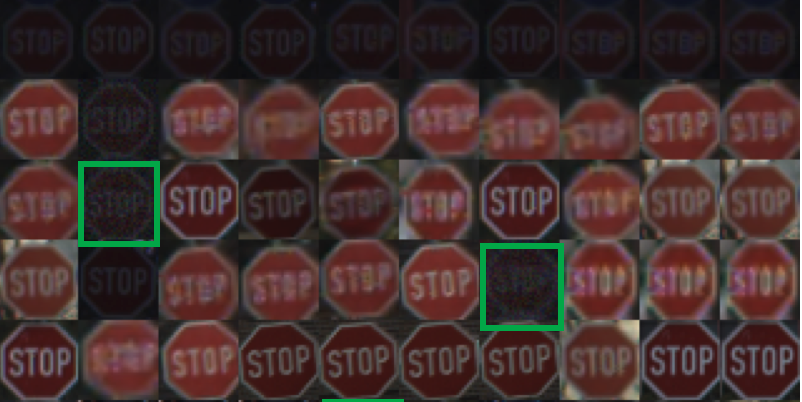
\includegraphics[width=.40\linewidth]{images/most_normalGtsrb}%
}\hspace{0.5cm}
\subfloat[Top 50 anomalous samples. \label{sfig:anomalousGtsrb}]{%
  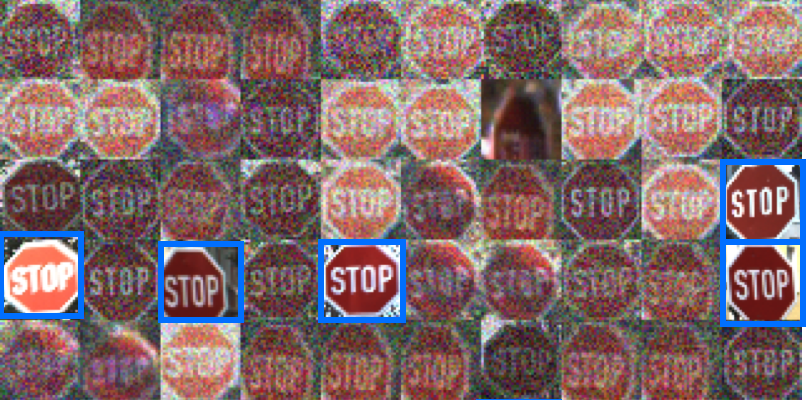
\includegraphics[width=.40\linewidth]{images/most_anomalousGtsrb}%
}
\caption{Most normal and anomalous stop signs detected by RCAE. Adversarial examples are highlighted in green, Normal samples are highlighted in blue}
\label{fig:gtsrbrcaeresults}
\end{figure*}
%  End of the Figure


% Results for Most anomalous and most normal images detected for GTSRB dataset
\begin{figure*}
\subfloat[Top 50 normal samples.. \label{sfig:normalGtsrb}]{%
  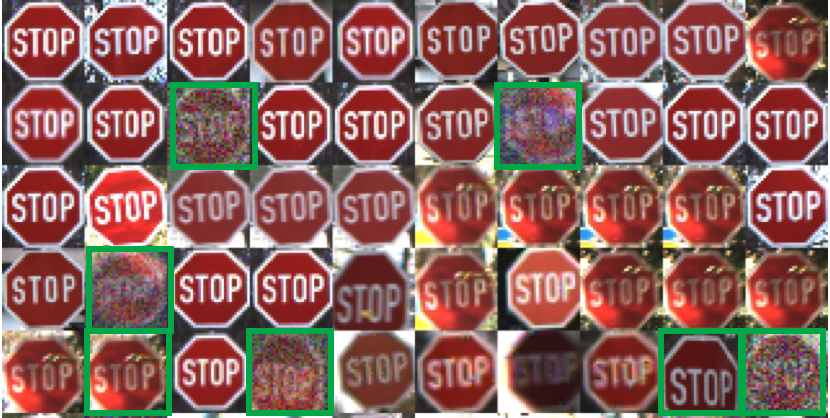
\includegraphics[width=.40\linewidth]{images/most_normalGtsrbocnn}%
}\hspace{0.5cm}
\subfloat[Top 50 anomalous samples. \label{sfig:anomalousGtsrb}]{%
  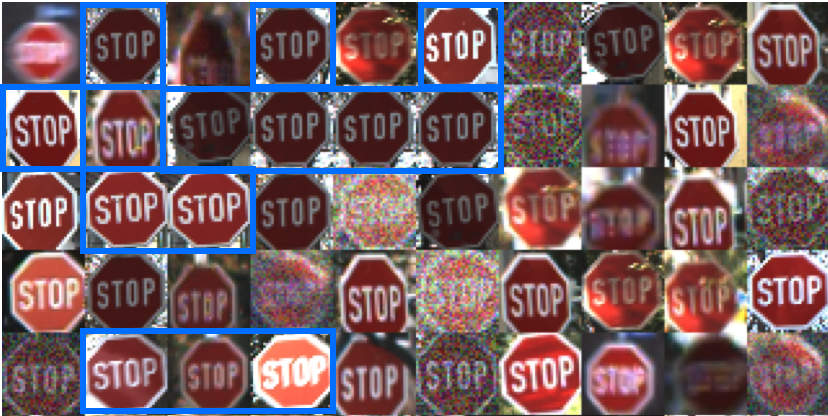
\includegraphics[width=.40\linewidth]{images/most_anomalousGtsrbocnn}%
}
\caption{Most normal and anomalous stop signs detected by OC-NN.  Adversarial examples are highlighted in green, Normal samples are highlighted in blue}
\label{fig:gtsrbocnnresults}
\end{figure*}
%  End of the Figure

% !TEX root=../main.tex
\section{Conclusion}
\label{sec:ocnn_conclusion}
In this paper, we have proposed a one-class neural network (OC-NN) approach for anomaly detection.
OC-NN uses a one-class SVM (OC-SVM) like loss function to train a neural network.
The advantage of OC-NN is that the features of the hidden layers are constructed for the specific
task of anomaly detection. This approach is substantially different from recently proposed
hybrid approaches which use deep learning features as input into an anomaly detector.  Feature
extraction in hybrid approaches is generic and not aware of the anomaly detection task. To learn
the parameters of the OC-NN network we have proposed a novel alternating minimization approach and
have shown that the optimization of a subproblem in OC-NN is equivalent to a quantile selection
% problem. Experiments on complex image and sequential data sets demonstrates that OC-NN is
% highly accurate. For future work, we would like to build and deploy an end to end system for anomaly
% detection based on OC-NN.







%Chapter-4 Unsupervised  DAD
% !TEX root=../main.tex
\chapter{Unsupervised Deep Anomaly Detection Methods}
\label{chpt:unsupervisedDAD}
\section{Introduction}

A common need when analysing real-world datasets is determining which instances stand out as being dramatically dissimilar to all others.
Such instances are known as \emph{anomalies}, and the goal of \emph{anomaly detection} (also known as \emph{outlier detection}) is to determine all such instances in a data-driven fashion~\cite{chandola2007outlier}.
Anomalies can be caused by errors in the data but sometimes are indicative of a new, previously unknown, underlying process;
in fact Hawkins~\cite{hawkins} defines an outlier as an observation that {\it deviates so significantly from other observations as to arouse suspicion that it was generated by a different mechanism.}

Principal Component Analysis (PCA) \cite{Hotelling:1933} is a core method for a range of statistical inference tasks, including anomaly detection.
The basic idea of PCA is that while many data sets are high-dimensional, they tend to inhabit a {low-dimensional manifold}.
PCA thus operates by (linearly) projecting data into a lower-dimensional space, so as to separate the {\em signal} from the {\em noise};
a data point which is far away from its projection is deemed as anomalous.

While intuitive and popular, PCA has limitations as an anomaly detection method.
Notably, it is highly sensitive to data perturbation: one extreme data point can completely change the orientation of the projection, often leading to the masking of anomalies.
A variant of PCA, known as a \emph{robust} PCA (RPCA) limits the impact of anomalies by using a clever decomposition of the data matrix~\cite{candes2010robust}.
We will discuss RPCA in detail in Section~\ref{sec:background},
but note here that it still carries out a linear projection,
and further cannot be used to make predictions on test instances;
that is, we cannot perform \emph{inductive} anomaly detection.

In this paper, we will relax the linear projection limitation of RPCA by using a deep and robust autoencoder~\cite{vincent2010stacked,Goodfellow-et-al-2016}.
The difference between RPCA and a deep autoencoder will be the use of a nonlinear activation function and the potential use of several hidden layers in the autoencoder.
While this modification is conceptually simple, we show it yields noticeable improvements in anomaly detection performance on complex real-world image data, where a linear projection cannot capture sufficient structure in the data.
Further, the robust autoencoder is capable of performing inductive anomaly detection, unlike RPCA.

\begin{comment}
Figure~\ref{mse} shows the output of using a robust and deep autencoder
to recover images. The data set consists of images of dogs where each
image has been corrupted with a small amount of noise. The proposed
autoencoder is able to reconstruct the dog images but fails to
properly reconstruct an image which has a dog and a boy. In fact,
the image of the dog with the boy was discovered as part of the
anomaly detection process using autoencoders.
\begin{figure}[!t]
	\centering
	\includegraphics[scale=0.5]{images/otherClass}
	\caption{Illustration of the  anomaly detection capability of deep inductive convolutional autoencoders.
		The data set consists of ``dog'' images (first column).
		Our proposed robust autoencoder decomposes an image $\X = \hat{\X} + \N$.
		The $\hat{\X}$ (second column) shows the reconstructed image and $\N$ (third column) shows the difference between the original and the reconstructed image.
		In the first row, a dog image is normal, while in the second row, an image of a flight  (an anomaly) is  reconstructed with high mean square error.}
	\label{mse}
	\vspace{-\baselineskip}
\end{figure}
\end{comment}

In the sequel,
we provide an overview of anomaly detection methods (Section~\ref{sec:related}), with a specific emphasis on matrix decomposition techniques
such as PCA and its robust extensions.
We then proceed to describe our proposed model based on autoencoders (Section~\ref{sec:method}),
and present our experiment setup and results (Section~\ref{sec:experiment-setup}, \ref{sec:experiment-results}).
Finally, we describe directions for future work (Section~\ref{sec:conclusion}).

% !TEX root=../main.tex
\section{Related Work}
\label{unsupervisedDAD:RelatedWork}

Consider a feature matrix $\X \in \Real^{N \times D}$,
where $N$ denotes the number of data points and $D$ the number of features for each point.
For example, $N$ could be the number of images in some photo collection, and $D$ the number of pixels used to represent each image.
The goal of anomaly detection is to determine which rows of $\X$ are anomalous, in the sense of being dissimilar to all other rows.
We will use $\X_{i :}$ to denote the $i$th row of $\X$.

%
\subsection{A tour of anomaly detection methods}

Anomaly detection is a widely researched topic in the data mining and machine learning community~\cite{chandola2007outlier,charubook}.
The two primary strands of research have been the design of novel algorithms to detect anomalies,
and the design \emph{efficient} means of discovering all anomalies in a large dataset.
In the latter strand, starting from the work of Bay and Schwabacher~\cite{bay03}, several optimisations have been proposed to discover anomalies in near linear time~\cite{Ghoting:2008}.

In the former strand, which is our primary focus, most emphasis has been on non-parametric methods like distance and density based outliers~\cite{knorr1997unified,breunig2000lof}.
For example, distance-based methods define a domain-dependent dissimilarity metric, and deem a point to be anomalous if it is relatively far away from its neighbours~\cite{Zhao:2009}.
Another popular approach is the one-class SVM, which learns a smooth boundary that captures the majority of probability mass of the data~\cite{Scholkopf:2001}.


In recent years,
matrix factorization methods for anomaly detection have become popular.
These methods provide a \emph{reconstruction matrix} $\hat{\X} \in \Real^{N \times D}$ of the input $\X$, and use the norm $\| \X_{i :} - \hat{\X}_{i :} \|_2^2$ as a measure of how anomalous a particular point $\X_{i :}$ is;
if the reconstruction is close to the input, then it is deemed normal;
else, anomalous.
We describe several popular examples of this approach, beginning with principal component analysis (PCA).



%
\subsection{PCA for anomaly detection}

PCA finds the directions of maximal variance of the data.
Supposing without loss of generality that the data matrix $\X$ has zero mean,
this may be understood as the result of a matrix factorisation \cite{Bishop:2006}:
\begin{equation}
	\label{eqn:pca}
	\min_{\W^T \W = \I, \Z} \| \X - \W \Z \|_F^2 = \min_{\U} \| \X - \X \U \U^T \|_F^2.
\end{equation}
Here,
the reconstruction matrix is $\hat{\X} = \X \U \U^T$,
where
$\U \in \Real^{D \times K}$ for some number of \emph{latent dimensions} $K \ll D$.
We can interpret $\X \U$ as a projection (or encoding) of $\X$ into a $K$-dimensional subspace,
with the application of $\U^T$ as an inverse projection (or decoding) back into the original $D$ dimensional space.


%
\subsection{Autoencoders for anomaly detection}

PCA assumes a linear subspace explains the data.
To relax this assumption, consider instead
\begin{equation}
	\label{eqn:autoencoder}
	\min_{\U, \V} \| \X - f( \X \U ) \V \|_F^2
\end{equation}
for some non-decreasing \emph{activation function} $f \colon \Real \to \Real$,
and $\U \in \Real^{D \times K}, \V \in \Real^{K \times D}$.
For the purposes of anomaly detection, one can define the reconstruction matrix as $\hat{\X} = f( \X \U ) \V$.

Equation \ref{eqn:autoencoder} corresponds to an autoencoder with a single hidden layer \cite{Goodfellow-et-al-2016}.
Popular choices of $f( \cdot )$ include the sigmoid $f( a ) = (1 + \exp(-a))^{-1}$ and the rectified linear unit or ReLU $f( x ) = \max(0, a)$.
As before, we can interpret $\X \U$ as an encoding of $\X$ into a $K$-dimensional subspace; however,
by applying a nonlinear $f( \cdot )$,
the projection is implicitly onto a nonlinear manifold.


%
\subsection{Robust PCA}

Another way to generalise PCA is to solve, for a tuning parameter $\lambda > 0$,
\begin{equation}
	\label{eqn:robust-pca}
	\min_{\S, \N} \| \S \|_* + \lambda \cdot \| \N \|_1 : \X = \S + \N,
\end{equation}
where $\| \cdot \|_*$ denotes the trace or nuclear norm $\| \X \|_* = \mathrm{tr}( (\X^T \X)^{1/2} )$,
and $\| \cdot \|_1$ the elementwise $\ell_1$ norm.
For the purposes of anomaly detection, one can define the reconstruction matrix $\hat{\X} = \X - \N = \S$.

Intuitively, Equation \ref{eqn:robust-pca} separates $\X$ into a signal matrix $\S$ and a noise matrix $\N$,
where the signal matrix has low-rank structure, and the noise is assumed to not overwhelm the signal for most of the matrix entries.
The trace norm may be seen as a convex relaxation of the rank function;
thus, this objective can be understood as a relaxed version of PCA.

Equation \ref{eqn:robust-pca} corresponds to robust PCA (RPCA)~\cite{candes2010robust}.
Unlike standard PCA, this objective can effortlessly deal with a single entry perturbed arbitrarily.
When $\lambda \to +\infty$, we will end up with $\N = \mathbf{0}, \S = \X$,
i.e.\, we will claim that there is no noise in the data, and so all points are deemed normal.
On the other hand, when $\lambda \to 0$, we will end up with $\N = \X, \S = \mathbf{0}$,
i.e.\, we will claim that there is no signal in the data, and so points with high norm are deemed anomalous.


%
\subsection{Direct robust matrix factorization}

Building upon RPCA,
Xiong et. al.~\cite{xiong2011direct} introduced the direct robust matrix factorization method (DRMF),
where for tuning parameters $K, e$ one solves:
\begin{equation}
	\label{eqn:drmf}
	\begin{aligned}
	\min_{\S, \N} \hspace{0.5cm} & \| \X - (\N + \S) \|_{F}^2 \colon \mbox{rank}(\S) \leq K, \|\N\|_{0} \leq e.
	\end{aligned}
\end{equation}
As before, the matrix $\N$ captures the anomalies and $\S$ captures the signal.
Unlike RPCA, one explicitly constraints $\S$ to be low-rank, rather than merely having low trace norm;
and one explicitly constraints $\N$ to have a maximal number of nonzeros, rather than merely having bounded $\ell_1$ norm.
The lack of convexity of the objective requires a bespoke algorithm for the optimisation.


%
\subsection{Robust kernel PCA}

Another way to overcome the linear assumption of PCA is the robust kernel PCA (RKPCA) approach of~\cite{Nguyen:2009}.
For a feature mapping $\Upphi$ into a reproducing kernel Hilbert space, and projection operator $\mathbf{P}$ of a point into the KPCA subspace, it is proposed to reconstruct an input $\mathbf{x} \in \Real^D$ by solving the pre-image problem
\begin{equation}
	\label{eqn:rkpca}
	\hat{\mathbf{x}} = \underset{\mathbf{z} \in \Real^D}{\mathrm{argmin}} \, E_0( \mathbf{x}, \mathbf{z} ) + C \cdot \| \Upphi( \mathbf{z} ) - \mathbf{P} \Upphi( \mathbf{z} ) \|^2,
\end{equation}
where $E_0$ is a robust measure of reconstruction error (i.e.\ not merely the Euclidean norm),
and $C > 0$ is a tuning parameter.
RKPCA does not explicitly handle gross outliers, unlike RPCA;
however, by choosing a rich feature mapping $\Upphi$, %(e.g.\ corresponding to a Gaussian kernel),
one can capture nonlinear anomalies.
This choice of feature mapping must be pre-specified, whereas autoencoder methods implicitly \emph{learn} a good mapping.

% !TEX root=../main.tex
\section{The Proposed Approach}
\label{sec:method}

We now present our robust (convolutional) autoencoder model for anomaly detection.
The method can be seen as an extension of robust PCA to allow for a nonlinear manifold that explains most of the data.

%
\subsection{Robust (convolutional) autoencoders}

Let $f \colon \Real \to \Real$ be some non-decreasing {activation function}.
Now consider the following objective, which combines the salient elements of Equations \ref{eqn:autoencoder} and \ref{eqn:robust-pca}:
\begin{equation}
	\label{eqn:robust-ae}
	\min_{\U, \V, \N} \| \X - (f(\X \U) \V + \N) \|_F^2 + \frac{\mu}{2} \cdot (\| \U \|_F^2 + \| \V \|_F^2) + \lambda \cdot \| \N \|_1,
\end{equation}
where $f( \cdot )$ is understood to act elementwise, and $\lambda, \mu > 0$ are tuning parameters.
This is a form of \emph{robust autoencoder}:
one encodes the input into the latent representation $\Z = f( \X \U )$,
which is then decoded via $\V$.
The additional $\N$ term captures gross outliers in the data, as with robust PCA.
For the purposes of anomaly detection, we have reconstruction matrix $\hat{\X} = f(\X \U) \V$.

When $\lambda \to +\infty$, we get $\N = \mathbf{0}$, and the model reduces to a standard autoencoder (Equation \ref{eqn:autoencoder}).
When $\lambda \to 0$, then one possible solution is $\N = \X$ and $\U = \V = \mathbf{0}$, so that the model memorises the training data.
For intermediate $\lambda$, the model augments a standard autoencoder with a noise absorption term that endows robustness.

More generally, Equation \ref{eqn:robust-ae} can be seen as an instance of
\begin{equation}
	\label{eqn:robust-cae}
	\min_{\theta, \N} \| \X - (\hat{\X}( \theta ) + \N) \|_F^2 + \frac{\mu}{2} \cdot \mathrm{\Omega}( \theta ) + \lambda \cdot \| \N \|_1,
\end{equation}
where $\hat{\X}( \theta )$ is some generic predictor with parameters $\theta$, and $\mathrm{\Omega}( \cdot )$ a regularisation function.
Observe that we could pick $\hat{\X}( \theta )$ to be a convolutional autoencoder~\cite{Jain:2008,vincent2010stacked}, which would be suitable when dealing with image data;
such a model will be studied extensively in our experiments.
Further, the regulariser $\mathrm{\Omega}$ could involve more general matrix norms, such as the $\ell_{1,2}$ norm \cite{Huang:2010}.


%
\subsection{Training the model}
\label{sec:training}

The objective function of the model of Equation \ref{eqn:robust-ae}, \ref{eqn:robust-cae} is non-convex, but unconstrained and sub-differentiable.
There are several ways of performing optimisation.
For example, for differentiable activation $f$, one could compute sub-gradients with respect to all model parameters and apply backpropagation.
However, to leverage existing advances in training deep networks, we observe that:
\begin{itemize}
	\item For fixed $\N$, the objective is equivalent to that of a standard (convolutional) autoencoder on the matrix $\X - \N$.
	Thus, one can optimise the parameters $\theta$ using any modern (stochastic) optimisation tool for deep learning that exploits gradients, such as Adam \cite{kingma2014adam}.

	\item For fixed $\theta$ (i.e.\, $\U, \V$ in the standard autoencoder case), the objective is
	$$ \min_{\theta, \N} \| \N - (\X - \hat{\X}( \theta )) \|_F^2 + \lambda \cdot \| \N \|_1, $$
	which trivially solvable via the soft thresholding operator on the matrix $\X - \hat{\X}( \theta )$ \cite{Bach:2011}, with solution
	$$ \N_{ij} =
	\begin{cases}
		(\X - \hat{\X}( \theta ))_{ij} - \frac{\lambda}{2} & \text{ if } (\X - \hat{\X}( \theta ))_{ij} > \frac{\lambda}{2} \\
		(\X - \hat{\X}( \theta ))_{ij} + \frac{\lambda}{2} & \text{ if } (\X - \hat{\X}( \theta ))_{ij} < -\frac{\lambda}{2} \\
		0 & \text{ else. }
	\end{cases}
	$$
\end{itemize}
We thus alternately optimise $\N$ and $\theta$ until the change in the overall objective is below some threshold.
The use of stochastic optimisation for the first step, and the simplicity of the optimisation for the second step, means that we can easily train the model where data arrives in an online or streaming fashion.


%
\subsection{Predicting with the model}

One convenient property of our model is that the anomaly detector will be inductive, i.e.\ it can generalise to unseen data points.
One can interpret the model as learning a robust representation of the input, which is unaffected by gross noise;
such a representation should thus be able to accurately model any unseen points that lie on the same manifold as the data used to train the model.

Formally, given a new $\mathbf{x}_* \in \Real^D$, one simply computes $f( \mathbf{x}_*^T \U ) \V$ to score this point.
The larger $\| \mathbf{x}_* - \V^T f( \U^T \mathbf{x}_* ) \|_2^2$ is, the more likely the point is deemed to be anomalous.
We emphasise that such inductive predictions are simply not possible with the robust PCA method, as it estimates parameters for the $N \times D$ observations present in $\X$, with no means of generalising to unseen data.



%
\subsection{Connection to robust PCA}

While the robust autoencoder of Equation \ref{eqn:robust-ae} has clear conceptual similarity to robust PCA,
it may seem that choices such as the $\ell_2$ penalty on $\U, \V$ are somewhat arbitrarily used in place of the trace norm.
We now show how the objective can in fact be naturally derived as an extension of RPCA.

The trace norm can be represented in the variational form~\cite{recht2010guaranteed}
$ \| \S \|_* = \min_{\W \V = \S} \frac{1}{2} \cdot (\| \W \|_F^2 + \| \V \|_F^2). $
The robust PCA objective is thus equivalently
$$ \min_{\W, \V, \N} \frac{1}{2} \cdot (\| \W \|_F^2 + \| \V \|_F^2) + \lambda \cdot \| \N \|_1 : \X = \W \V + \N. $$
This objective has the disadvantage of being non-convex,
but the advantage of being amenable to extensions.
Pick some $\mu > 0$, and consider a relaxed version of the robust PCA objective:
$$ \min_{\W, \V, \N, \E} \| \E \|_F^2 + \frac{\mu}{2} \cdot (\| \W \|_F^2 + \| \V \|_F^2) + \lambda \cdot \| \N \|_1 : \X = \W \V + \N + \E. $$
Here, we allow for further systematic errors $\E$
which have low average magnitude.
We can equally consider the unconstrained objective
\begin{equation}
	\label{eqn:rpca-v2}
	\min_{\W, \V, \N} \| \X - (\W \V + \N) \|_F^2 + \frac{\mu}{2} \cdot (\| \W \|_F^2 + \| \V \|_F^2) + \lambda \cdot \| \N \|_1
\end{equation}
This re-expression of robust PCA has been previously noted, for example in Sprechmann et al.~\cite{Sprechmann:2015}.
To derive the robust autoencoder from Equation \ref{eqn:rpca-v2}, suppose now that we constrain $\W = \X \U$.
This is a natural constraint in light of Equation \ref{eqn:pca}, since for standard PCA we factorise $\X$ into $\hat{\X} = \X \U \U^T$.
Then, we have the objective
$$ \min_{\U, \V, \N} \| \X - (\X \U \V + \N) \|_F^2 + \frac{\mu}{2} \cdot (\| \X \U \|_F^2 + \| \V \|_F^2) + \lambda \cdot \| \N \|_1. $$
Now suppose we modify the regulariser to only operate on $\U$ rather than $\X \U$:
$$ \min_{\U, \V, \N} \| \X - (\X \U \V + \N) \|_F^2 + \frac{\mu}{2} \cdot (\| \U \|_F^2 + \| \V \|_F^2) + \lambda \cdot \| \N \|_1. $$
This is again natural in the context of standard PCA, since there we have $\W = \X \U$ satisfying $\W^T \W = \I$.
Observe now that we have derived Equation \ref{eqn:robust-ae} for a linear activation function $f( x ) = x$.
The robust autoencoder thus extends this model by employing a nonlinear activation.


%
\subsection{Relation to existing models}

Our contribution is a nonlinear extension of RPCA for anomaly detection.
As noted above, the key advantages over RPCA are the ability to capture nonlinear structure in the data, as well as the ability to detect anomalies in an inductive setting.
The price we have to pay is the lack of convexity of the objective function, unlike RPCA;
nonetheless, we shall demonstrate that the model can be effectively trained using the procedure described in Section \ref{sec:training}.

Some works have employed deep networks for anomaly detection~\cite{Williams:2002,Zhai:2016},
but without explicitly accounting for gross anomalies.
For example, the recent work of \cite{Zhai:2016} employed an autoencoder-inspired objective to train a probabilistic neural network, with extensions to structured data;
the use of an RPCA-style noise matrix $\N$ may be useful to explore in conjunction with such methods.

Our method is also distinct to denoising autoencoders (DNA), wherein noise is explicitly added to instances~\cite{vincent2010stacked}, whereas we \emph{infer} the noise automatically.
The approaches have slightly different goals: DNAs aim to extract good features from the data, while our aim is to identify anomalies.

Finally, while nonlinear extensions of PCA-style matrix factorisation (including via autoencoders) have been explored in contexts such as collaborative filtering \cite{Lawrence:2009,Sedhain:2015}, we are unaware of prior usage for anomaly detection.

% !TEX root=../main.tex
\section{Experimental Setup}
\label{sec:unsup_experiment-setup}

In this section we show the empirical effectiveness of Robust Convolutional Autoencoder over the state-of-the-art methods on real-world data.
Our primary focus will be on non-trivial image datasets, although our method is applicable in any context where autoencoders are useful e.g.\ speech.

%\vspace{-0.3 cm}
\subsection{Methods compared}
%\vspace{-0.2 cm}
We compare our proposed Robust Convolutional Autoencoder (RCAE)
with the following  state-of-the art methods for anomaly detection:
\let\labelitemi\labelitemii
\begin{itemize}
	\item \textbf{Truncated SVD}, which for zero-mean features is equivalent to PCA. %We reused the code from
	%\url{http://scikit-learn.org/stable/modules/generated/sklearn.decomposition.TruncatedSVD.html}

	\item \textbf{Robust PCA (RPCA)}~\cite{candes2010robust}, as per Equation \ref{eqn:robust-pca}.

	\item \textbf{Robust kernel PCA (RKPCA)}~\cite{Nguyen:2009}, as per Equation \ref{eqn:rkpca}.

   	\item \textbf{Autoencoder (AE)}~\cite{bengio2009learning}, as per Equation \ref{eqn:autoencoder}.

   	\item \textbf{Convolutional Autoencoder (CAE)}, a convolutional autoencoder without any accounting for gross anomalies i.e. Equation \ref{eqn:robust-cae} where $\lambda = +\infty$.

   	\item \textbf{Robust Convolutional Autoencoder (RCAE)}, our proposed model as per Equation \ref{eqn:robust-cae}.
\end{itemize}
We used TensorFlow \cite{abadi2016tensorflow} for the implementation of AE, CAE and RCAE\footnote{\url{https://github.com/raghavchalapathy/rcae}}.
For RPCA and RKPCA,
we used
publicly available implementations\footnote{\url{http://perception.csl.illinois.edu/matrix-rank/sample_code.html}}\footnote{\url{http://www3.cs.stonybrook.edu/~minhhoai/downloads.html}}.

%\vspace{-0.3 cm}
\subsection{Datasets}
%%\vspace{-0.2 cm}
We compare all methods on three real-world datasets:
\begin{itemize}
	\item {\tt restaurant}, comprising video background modelling and activity detection consisting of snapshots of restaurant activities~\cite{xiong2011direct}.
	\item {\tt usps}, comprising the USPS handwritten digits~\cite{hull1994database}.
%	\item {\tt escalator}, comprising Surveillance camera subway station activities~\cite{becker2011templates}
	\item {\tt cifar-10} consisting of 60000 $32\times32$ colour images in 10 classes, with 6000 images per class~\cite{krizhevsky2009learning}.
\end{itemize}
For each dataset, we perform further processing to create a well-posed anomaly detection task, as described in the next section.

\subsection{Evaluation methodology}

As anomaly detection is an unsupervised learning problem, model evaluation is challenging.
For the {\tt restaurant} dataset, there are no ground truth anomalies, and so we perform a qualitative analysis by visually comparing the anomalies flagged by various methods, as done in the original robust PCA paper~\cite{candes2010robust}.

For the other two datasets,
we follow a standard protocol (see e.g.~\cite{xiong2011direct}) wherein anomalies are explicitly identified in the training set.
We can then evaluate the predictive performance of each method as measured against the ground truth anomaly labels,
using three standard metrics:
\begin{itemize}
	\item the area under the precision-recall curve (AUPRC)

	\item the area under the ROC curve (AUROC)

	\item the precision at 10 (P@10).
\end{itemize}
AUPRC and AUROC measure ranking performance, with the former being preferred under class imbalance \cite{Davis:2006}.
P@10 measures classification performance, being the fraction of the top 10 scored instances which are actually anomalous.

For $\tt{CIFAR-10}$,
the labelled dataset is created by combining 5000 images of dogs and 50 images of cats;
a good anomaly detection method should thus flag the cats to be anomalous.
Similarly,
for $\tt{usps}$,
the dataset is created by
a mixture of 220 images of \lq1\rq s, and 11 images of \lq7\rq as in~\cite{xu2010robust}.
Details of the datasets are summarised in Table \ref{tbl:datasets}.

\begin{table}[!t]
	\centering
	\renewcommand{\arraystretch}{1.25}
	\setlength{\tabcolsep}{6pt}
	%\scalebox{0.85}{
	\begin{tabular}{@{}llll@{}}
		\toprule
		\toprule
		Dataset & \# instances & \# anomalies & \# features \\
		\toprule
		{\tt restaurant} & 200 & Unknown (foreground) & 19200 \\
		%		{\tt escalator}  & 200 & 50 & 20800 \\
		{\tt usps} 		 & 231 & 11 (\lq7\rq) & 256 \\
		{\tt cifar-10} 	 & 5000 & 50 (cats) & 1024 \\
		\bottomrule
	\end{tabular}
	%}
	%\vspace{0.1 cm}
	\caption{Summary of datasets used in experiments.}
	\label{tbl:datasets}
	%\vspace{-\baselineskip}
\end{table}

Additionally,
we also test the ability of our model to perform denoising of images,
as well as detecting inductive anomalies.


\subsection{Network parameters}

Although we have observed that deeper RCAE networks tend to achieve better image reconstruction performance, there exist four fold options related to network parameters to be chosen:
(a) number of convolutional filters, (b) filter size, (c) strides of convolution operation and (d) activation applied.
We tuned via grid search additional hyper-parameters, including the number of hidden-layer nodes $H \in \{3, 64, 128\}$, and regularisation $\lambda$ within range ${[0, 100]}$.
The learning, drop-out rates and regularization parameter $\mu$ were sampled from a uniform distribution in the range $[0.05, 0.1]$.
The embedding and initial weight matrices were all sampled from the uniform distribution within range $[-1, 1]$.


\section{Experimental Results}
\label{sec:unsup_experiment-results}

In this section, we present experiments for three scenarios:
(a) non-inductive anomaly detection,
(b) inductive anomaly detection, and
(c) image denoising.

%\vspace{-0.3 cm}
%%%
\subsection{Non-inductive anomaly detection results}

We present results on the three datasets described in Section \ref{sec:experiment-setup}.


%%%
\subsubsection{{(1) {\tt restaurant} dataset}}
We work with the {\tt restaurant} video activity detection dataset~\cite{xiong2011direct},
and consider the problem of inferring the background of videos via removal of (anomalous) foreground pixels.
Estimating the background in videos is important for tasks such as anomalous activity detection.
It is however difficult because of the variability of the background (e.g. due to lighting conditions) and the presence of foreground objects such as moving objects and people.

For this experiment, we only compare the RPCA and RCAE methods, owing to a lack of ground truth labels.

\textbf{Parameter settings}.
For RPCA, rank $K$ = 64 is used.

Per the success of the Batch Normalization architecture~\cite{ioffe2015batch} and Exponential Linear Units~\cite{clevert2015fast}, we have found that convolutional+batch-normalization+elu layers provide a better representation of convolutional filters.
Hence, in this experiment the RCAE adopts four layers of (conv-batch-normalization-elu) in the encoder part and four layers of  (conv-batch-normalization-elu) in the decoder portion of the network.
RCAE network parameters such as (number of filter, filter size, strides) are chosen to be (16,3,1) for first and second layers and (32,3,1) for third and fourth layers of both encoder and decoder layers.

\begin{figure}[!t]
	\centering
	\subfigure[RCAE.]{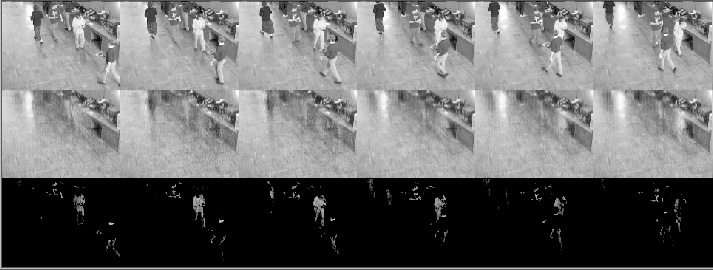
\includegraphics[scale=0.325]{images/Restaurant/CAE_worst.jpg}}
	\subfigure[RPCA.]{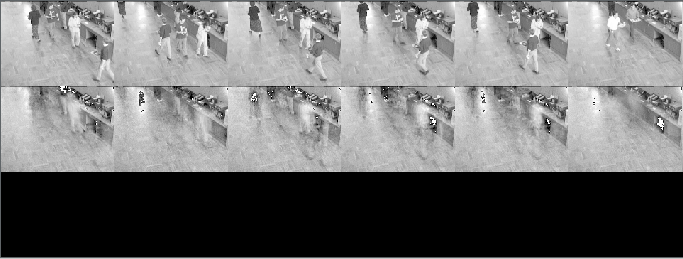
\includegraphics[scale=0.325]{images/Restaurant/RPCA_worst.jpg}}
	\caption{Top anomalous images containing original image (people walking in the lobby) decomposed into background (lobby) and foreground (people), {\tt restaurant} dataset.}
	\label{fig:results-restaurant}
\end{figure}

%\vspace{-0.3 cm}
\textbf{Results}.
While there are no ground truth anomalies in this dataset, a qualitative analysis reveals RCAE to outperforms its counterparts in capturing the foreground objects.
Figure~\ref{fig:results-restaurant} compares the top 6 most anomalous images for RCAE and RPCA.
We see that the most anomalous images contain high foregound activity (which are recognised as anomalous).
Visually, we see that the background reconstruction produced by RPCA contains a few blemishes in some cases, while for RCAE the backgrounds are smooth.


%%%
\subsubsection{{(2) {\tt usps} dataset}}
From the {\tt usps} handwritten digit dataset,
we create a dataset
with a mixture of 220 images of \lq1\rq s, and 11 images of \lq7\rq, as in~\cite{xu2010robust}.
Intuitively, the latter images are treated as being anomalous, as the corresponding images have different characteristics to the majority of the training data. Each image is flattened as a row vector, yielding a 231 $\times$ 256 training matrix.

\textbf{Parameter settings}.
For SVD and RPCA methods, rank $K = 64$ is used.
For AE, the inputs are flattened images as a column vector of size 256,
and the hidden layer is a column vector of size  64 (matching the rank $K$).

For DRMF, we follow the settings of~\cite{xu2010robust}.
For RKPCA, we used a Gaussian kernel with bandwidth $0.01$, a cost parameter $C = 1$, and requested $60\%$ of the KPCA spectrum (which roughly selects 64 principal components).

For RCAE, we set two layers of convolution layers with the filter number to be 32, filter size to be 3$\times$3, with number of strides as $1$ and  rectified linear unit (ReLU) as activation with max-pooling layer of dimension 2$\times$2.

\textbf{Results}.
From Table~\ref{tbl:anomaly-results-summary}, we see that it is a near certainty for all \lq7\rq\, are accurately identified as outliers.
Figure~\ref{fig:usps-anomalies} shows the top anomalous images for RCAE, where indeed the \lq7\rq's are correctly placed at the top of the list.
By contrast, for RPCA there are also some \lq1\rq's placed at the top.

\begin{figure}[!t]
	\centering
	\subfigure[RCAE.]{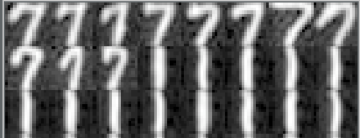
\includegraphics[scale=0.9]{usps-anomalies-crop}}
	\quad
	\subfigure[RPCA.]{\includegraphics[scale=0.29]{rpca_usps}}
	\caption{Top anomalous images, {\tt usps} dataset.}
	\label{fig:usps-anomalies}
	%\vspace{-\baselineskip}
\end{figure}

\begin{table*}[!t]
	\centering
	\renewcommand{\arraystretch}{1.25}
	\resizebox{0.99\linewidth}{!}{
	\subfigure[{\tt usps}]{
		\begin{tabular}{lccc}
			\toprule
			\toprule
			\textbf{Methods} & \textbf{AUPRC} & \textbf{AUROC} & \textbf{P@10} \\
			\midrule
			RCAE  & \cellcolor{gray!25}{0.9614 $\pm$ 0.0025}&\cellcolor{gray!25}{0.9988$\pm$ 0.0243}&\cellcolor{gray!25}{0.9108 $\pm$ 0.0113} \\
			\midrule
			CAE & 0.7003 $\pm$ 0.0105 & 0.9712 $\pm$ 0.0002 & 0.8730 $\pm$ 0.0023\\
			AE  & 0.8533 $\pm$ 0.0023 & 0.9927 $\pm$ 0.0022 & 0.8108 $\pm$ 0.0003 \\
			\midrule
			RKPCA & 0.5340 $\pm$ 0.0262 & 0.9717 $\pm$ 0.0024 & 0.5250 $\pm$ 0.0307 \\
			DRMF  & 0.7737 $\pm$ 0.0351 & 0.9928 $\pm$ 0.0027 & 0.7150 $\pm$ 0.0342 \\
			RPCA  & 0.7893 $\pm$ 0.0195 & 0.9942 $\pm$ 0.0012 & 0.7250 $\pm$ 0.0323\\
			SVD   & 0.6091 $\pm$ 0.1263 & 0.9800 $\pm$ 0.0105 & 0.5600 $\pm$ 0.0249 \\
			\bottomrule
	\end{tabular}}%
	\quad
	\subfigure[{\tt cifar-10}]{
		\begin{tabular}{ccc}
			\toprule
			\toprule
			\textbf{AUPRC} & \textbf{AUROC} & \textbf{P@10} \\
			\midrule
			\cellcolor{gray!25}{0.9934 $\pm$ 0.0003}&\cellcolor{gray!25}{0.6255 $\pm$ 0.0055} &\cellcolor{gray!25}{0.8716 $\pm$ 0.0005} \\
			\midrule
			0.9011 $\pm$ 0.0000 & 0.6191 $\pm$ 0.0000 & 0.0000 $\pm$ 0.0000 \\
			0.9341 $\pm$ 0.0029 & 0.5260 $\pm$ 0.0003 & 0.2000 $\pm$ 0.0003 \\
			\midrule
			0.0557 $\pm$ 0.0037 & 0.5026 $\pm$ 0.0123 & 0.0550 $\pm$ 0.0185 \\
			0.0034 $\pm$ 0.0000 & 0.4847 $\pm$ 0.0000 & 0.0000 $\pm$ 0.0000 \\
			0.0036 $\pm$ 0.0000 & 0.5211 $\pm$ 0.0000 & 0.0000 $\pm$ 0.0000 \\
			0.0024 $\pm$ 0.0000 & 0.5299 $\pm$ 0.0000 & 0.0000 $\pm$ 0.0000 \\
			\bottomrule
	\end{tabular}}%
	}

	\caption{Comparison between the baseline (bottom four rows) and state-of-the-art systems (top three rows). Results are the mean and standard error of performance metrics over 20 random training set draws. Highlighted cells indicate best performer.}
	\label{tbl:anomaly-results-summary}
	%\vspace{-0.2in}
\end{table*}

\subsubsection{{(3) {\tt cifar-10} dataset}}
We create a dataset with anomalies
by combining 5000 random images of dogs and 50 images of cats, as illustrated in Figure~\ref{fig:results-cifar}.
In this scenario the cats are anomalies, and the goal is to detect all the cats in an unsupervised manner.

\textbf{Parameter settings}.
For SVD and RPCA methods, rank $K = 64$ is used.
We trained a three-hidden-layer autoencoder (AE) (1024-256-64-256-1024 neurons).
The middle hidden layer size is set to be same as rank $K = 64$, %(same as number of components used in SVD and RPCA),
and the model is trained using Adam~\cite{kingma2014adam}.
The decoding layer uses sigmoid function in order to capture the nonlinearity characteristics from  latent representations produced by the hidden layer.
Finally, we obtain the feature vector for each image by obtaining the latent representation from the hidden layer.

For RKPCA, we used a Gaussian kernel with bandwidth $5 \cdot 10^{-8}$, a cost parameter $C = 0.1$, and requested $55\%$ of the KPCA spectrum (which roughly selects 64 principal components).
The RKPCA runtime was prohibitive on the full sample (see Sec \ref{sec:runtime}), so we resorted to a subsample of 1000 dogs and 50 cats.

The RCAE architecture in this experiment is same as for {\tt restaurant}, containing
four layers of  (conv-batch-normalization-elu) in the encoder part
and four layers of  (conv-batch-normalization-elu) in the decoder
portion of the network. RCAE network parameters such as (number of filter, filter size, strides) are chosen to be (16,3,1)  for first and second layers and (32,3,1) for third and fourth layers of both encoder and decoder.

\begin{figure}[!t]
	\centering
	\subfigure[RCAE.]{\includegraphics[scale=0.95]{images/CIFAR_10/CAE_worst_inductive_crop}}
	\subfigure[RPCA.]{\includegraphics[scale=0.95]{images/CIFAR_10/RPCA_worst_inductive_crop}}
	\caption{Top anomalous images, %along with background and foreground,
	{\tt cifar-10} dataset.}
	\label{fig:results-cifar}
\end{figure}

\textbf{Results}.
From Table \ref{tbl:anomaly-results-summary},
RCAE clearly outperforms all existing state-of-the art methods in anomaly detection.
Note that basic CAE, with no robustness (effectively $\lambda = \infty$), is also outperformed by our method, indicating that it is crucial to explicitly handle anomalies with the $\N$ term.

Figure~\ref{fig:results-cifar} illustrates the most anomalous images for our RCAE method, compared to RPCA.
Owing to the latter involving learning a linear subspace, the model is unable to effectively distinguish cats from dogs;
by contrast, RCAE can effectively determine the manifold characterising most dogs, and identifies cats to be anomalous with respect to this.


%%%%%%%%%
\subsection{Inductive anomaly detection results}

We conduct an experiment to assess the detection of \emph{inductive} anomalies.
Recall that this is a capability of our RCAE model, but not e.g. RPCA.
We consider the following setup:
we train our model on 5000 dog images, and then evaluate it on a test set comprising 500 dogs and 50 cat images.
As before, we wish all methods to accurately determine the cats to be anomalies.

\begin{figure}[!t]
	\centering
	\subfigure[RCAE.]{\includegraphics[scale=0.31]{images/CIFAR_10/caeInductiveAnomalies_crop.jpg}}
	\subfigure[CAE.]{\includegraphics[scale=0.95]{images/CIFAR_10/caeInductiveAnomalies_crop_new.jpg}}
	\caption{Top inductive anomalous images, {\tt cifar-10} dataset.}
	\label{fig:results-cifar-inductive}
\end{figure}


Table~\ref{tbl:inductive-anomaly-results} summarises the detection performance for all the methods on this inductive task.
The lower values compared to Table~\ref{tbl:anomaly-results-summary} are indicative that the problem here is more challenging than anomaly detection on a single dataset;
nonetheless, we see that our RCAE method manages to convincingly outperform both the SVD and AE baselines.
This is confirmed qualitatively in Figure~\ref{fig:results-cifar-inductive}, where we see that RCAE correctly identifies many cats in the test set as anomalous, while the basic
%AE
CAE
method suffers.

\begin{table}[!t]
	\centering
	\renewcommand{\arraystretch}{1.25}
	\caption{Inductive anomaly detection results on {\tt cifar-10}. Note that RPCA and DRMF are inapplicable here. Highlighted cells indicate best performer.}
	\resizebox{0.99\linewidth}{!}{
	\begin{tabular}{@{}lccccc@{}}
		\toprule
		\toprule
		& \textbf{SVD} & \textbf{RKPCA} & \textbf{AE} & \textbf{CAE} & \textbf{RCAE} \\
		\toprule
		\bf{AUPRC} & 0.1752 $\pm$ 0.0051 & 0.1006 $\pm$ 0.0045 & 0.6200 $\pm$ 0.0005 & 0.6423 $\pm$ 0.0005 & \cellcolor{gray!25}{0.6908 $\pm$ 0.0001} \\
		\bf{AUROC} & 0.4997 $\pm$ 0.0066 & 0.4988 $\pm$ 0.0125 & 0.5007 $\pm$ 0.0010 & 0.4708 $\pm$ 0.0003 & \cellcolor{gray!25}{0.5576 $\pm$ 0.0005} \\
		\bf{P@10}  & 0.2150 $\pm$ 0.0310 & 0.0900 $\pm$ 0.0228 & 0.1086 $\pm$ 0.0001 & 0.2908 $\pm$ 0.0001 & \cellcolor{gray!25}{0.5986 $\pm$ 0.0001} \\
		\bottomrule
	\end{tabular}
	}
	\label{tbl:inductive-anomaly-results}
\end{table}


%%%
\subsection{Image denoising results}

Finally, we test the ability of the model to de-noise images, which is a form of anomaly detection on individual pixels (or more generally, features).
In this experiment, we train all models on a set of 5000 images of dogs from {\tt cifar-10}.
For each image, we then add salt-and-pepper noise at a rate of 10\%.
Our goal is to recover the original image as accurately as possible.

Figure~\ref{fig:results-cifar-injection} illustrates that the most anomalous images in the presence of noise
contain images of the variations of dog class images (e.g. containing person's face).
Further, Figure \ref{fig:denoising-results} illustrates for various methods the mean square error between the reconstructed and original images.
RCAE effectively suppresses the noise as evident from the low error.
The improvement over raw CAE is modest, but suggests that there is benefit to explicitly accounting for noise.

%\vspace{-0.3 cm}
\begin{figure}[!t]
	\centering
	\subfigure[RCAE.]{\includegraphics[scale=0.95]{images/CIFAR_10/CAE_worst_crop.jpg}}
	\subfigure[RPCA.]{\includegraphics[scale=0.95]{images/CIFAR_10/RPCA_worst_crop.jpg}}
	\caption{Top anomalous images in original form (first row), noisy form (second row),
	image denoising task on {\tt cifar-10}.}
	\label{fig:results-cifar-injection}
\end{figure}

\begin{figure}[!t]
	\centering
	\includegraphics[scale=0.5]{images/cifar_10_mse.pdf}
	\caption{Illustration of the mean square error boxplots obtained for various models on image denoising task, {\tt cifar-10} dataset.
		In this setting, RCAE suppresses the noise and detects the background and foreground images effectively.}
	\label{fig:denoising-results}
	%\vspace{-\baselineskip}
\end{figure}


%%%
\subsection{Comparison of training times}
\label{sec:runtime}

We remark finally that our RCAE method is comparable in training efficiency to existing methods.
For example, on the small-scale {\tt restaurant} dataset, it takes 1 minute to train RPCA,
and 8.5 minutes to train RKPCA,
compared with 10 minutes for our RCAE method.
The ability to leverage recent advances in deep learning as part of our optimisation (e.g.\ training models on a GPU) is we believe a salient feature of our approach.

We note that while the RKPCA method is fast to train on smaller datasets, on larger datasets it suffers from the $O(n^2)$ complexity of kernel methods;
for example, it takes over an hour to train on the {\tt cifar-10} dataset.
It is plausible that one could leverage recent advances in fast approximations of kernel methods~\cite{Lopez-Paz:2014}, and studying these would be of interest in future work.
Note that the issue of using a fixed kernel function would remain, however.

% !TEX root=../main.tex
\section{Conclusion}
\label{sec:conclusion}

We have extended the robust PCA model to the nonlinear autoencoder setting.
To the best of our knowledge, ours is the first approach which is \emph{robust}, \emph{nonlinear} and \emph{inductive}.
The robustness ensures that the model is not over-sensitive
to anomalies;
the nonlinearity helps discover potentially more
subtle anomalies;
and being inductive makes it possible
to deploy our model in a live setting.

While autoencoders are a powerful mechansim for data representation
they suffer from their ``black-box'' nature. There is a growing
body of research on outlier description, i.e., explain the reason
why a data point is anomalous. A direction of future reason is
to extend deep autoencoders for outlier \emph{description}.



% Group Anomaly detection using DGM
% DGMs
\section[Deep Generative Models]{Group Anomaly Detection using Deep Generative Models \footnote{Joint paper where deep generative models are applied for detecting group anomalies. I specialise in formulating the deep generative models for group anomaly detection while Eddie specialise and describe the area of group anomaly detection.}
} \label{sec:dgm}
%\section{Introduction}
This chapter proposes deep generative models (DGMs) for solving the static group anomaly detection (GAD) problem. GAD is a non-trivial problem for many real-world applications especially for more complicated group distributions in image datasets.  Images can be considered as groups of pixels or visual features however it is difficult to characterise the statistical properties of images.  Xiong et al. \cite{FGM} propose a novel GAD method applied to image data  however we attempt to improve these results by applying DGMS as they are successfully applied in many high-dimensional datasets %
  \cite{schlegl2017unsupervised,xu2018unsupervised,an2015variational}.
      The GAD problem in image datasets is useful and applicable to similar real-world challenges where group distributions are more complex and difficult to characterise.

  Figure \ref{fig:GAD} depicts examples of  group anomalies where the innermost circle contains images exhibiting regular behaviours whereas the outer circle conveys group anomalies.
% For example, if regular groups represent cat images then tiger images are point-based  group anomalies while a rotated cat is a distribution-based group anomaly (rotated cat features).
 { Figure \ref{fig:GAD} (a) displays  anomalous  tiger images
as well as $180^\circ$ rotation of cat images. %with rotated distributions of visual cat features.
}  Plot (b) illustrates irregular mixtures of cats and dogs in a single image while plot (c) portrays anomalous images stitched  from different scene categories of cities, mountains and coastlines. %regular images involve  while the outer circle contains stitched images from different scenes.
Our image data experiments will mainly focus on detecting group anomalies in these scenarios.


 \begin{figure}[h]
%\includegraphics[scale=0.38]
\includegraphics[scale=0.5,%width=8.5cm, height=9.8cm,
trim=0.5cm 0.2cm 0.5cm 0.8cm]
%{inputGADAnomalies}
{GADExample}
\centering
\caption{ Examples of point-based and distribution-based group anomalies in our image data experiments. The regular group behaviours represents images in the inner concentric circle while the outer circle contains images that are group anomalies. %Mean embedding vector $\mu$ characterises the expected group pattern.
}
\label{fig:GAD}
\end{figure}



%%ASK1 {Challenges} in Image Application
%Even though the GAD for image datasets may seem like a straightforward comparison of images, many complications and challenges arise.
 Many additional complications and challenges arise in GAD for image data.
 As there is a dependency between the location of pixels in a high-dimensional space, appropriate features in an image are difficult to extract. An effective detection of group anomalies requires an adequate characterisation of images for model training.   Image quality is affected by factors include low resolution, poor illumination intensity, different viewing angles, different scaling and so on. % Another issue is that ground truth labels are usually unavailable for training or evaluation purposes so anomaly injection is usually applied.
 Pre-processing, feature extraction and other techniques may resolve some of these challenges.


In order to detect  group anomalies in various image applications, we propose using  deep generative models (DGMs).
The main contributions of this chapter are: %\vspace{-1mm}
\begin{itemize}
\item We formulate DGMs for the GAD problem  using a group reference function.   Although DGMs have been applied in various image applications, they have not been applied for GAD. % of detecting group anomalies.
\item  A comparison study is conducted  on both  synthetic and real-world datasets to demonstrate the effectiveness of  DGMs as compared to other GAD techniques. % that detect point-based anomalous images.
%\item {\bf Scalability:} DNN  can be rapid and scalable compared to other ...
\vspace{1mm}
\end{itemize}


\begin{comment}
Figure~\ref{mse} shows the output of using a robust and deep autoencoder
to recover images. The data set consists of images of dogs where each
image has been corrupted with a small amount of noise. The proposed
autoencoder is able to reconstruct the dog images but fails to
properly reconstruct an image which has a dog and a boy. In fact,
the image of the dog with the boy was discovered as part of the
anomaly detection process using autoencoders.
\begin{figure}[!t]
	\centering
	\includegraphics[scale=0.5]{otherClass}
	\caption{Illustration of the  anomaly detection capability of deep inductive convolutional autoencoders.
		The data set consists of ``dog'' images (first column).
		Our proposed robust autoencoder decomposes an image $\X = \hat{\X} + \N$.
		The $\hat{\X}$ (second column) shows the reconstructed image and $\N$ (third column) shows the difference between the original and the reconstructed image.
		In the first row, a dog image is normal, while in the second row, an image of a flight  (an anomaly) is  reconstructed with high mean square error.}
	\label{mse}
	\vspace{-\baselineskip}
\end{figure}
\end{comment}

The rest of the chapter is organised as follows. An overview of related work is provided (Section~\ref{DGM:RelatedWork}) and preliminaries for understanding approaches for detecting  group anomalies are described in Section~\ref{sec:preliminaries}.
We formulate the GAD problem and then proceed to elaborate on our proposed solution that involves deep generative models (Section~\ref{sec:method}).
Our experimental setup and key results are presented in Section~ \ref{sec:experiment-setup}  and Section ~\ref{sec:experiment-results} respectively.
Finally, Section~\ref{sec:conclusion} provides a summary of our findings. % as well as recommends future directions for GAD research.

% !TEX root=../main.tex
\section{Related Work} \label{DGM:RelatedWork}
GAD is an emerging area  of research where most state-of-the-art techniques have been more recently developed.  While group anomalies are briefly discussed in anomaly detection surveys such as Chandola et al. \cite{Chandola} and Austin \cite{Hodge},  
  Yu et al. \cite{SurveySocialMedia} elaborates on GAD techniques where group memberships are not previously known.  
   {  Recently Toth and Chawla \cite{MySurvey} provide a comprehensive overview of GAD methods as well as a detailed  description of detecting temporal changes in groups over time. 
}
We focus on group anomalies in image applications where group memberships are known a priori. 

Previous studies on image anomaly detection % involving image   applications 
can be understood in terms of group anomalies. 
%Anomaly detection has been  previously studied in a variety of image classification applications. 
Quellec et al.  \cite{mammo} examine mammographic images  where point-based group anomalies represent potentially cancerous regions. Perera and Patel \cite{chairs} learn features from a collection of images containing regular chair objects and detect point-based group anomalies where chairs have abnormal shapes, colors and other irregular characteristics. On the other hand, Xiong et al. \cite{FGM} detect distribution-based group anomalies that are stitched images from scene categories (inside city, mountain or coast). %At a pixel level,   Xiong et al. \cite{MGM} apply GAD methods to detect anomalous galaxy clusters with irregular proportions of RGB pixels. 
We emphasise detecting distribution-based group anomalies rather than point-based anomalies in our subsequent  image applications.

The discovery of group anomalies is of interest to a number of diverse domains.   
  Muandet et al.	\cite{OCSMM} investigate GAD for physical phenomena in high energy particle physics where Higgs bosons are observed as slight excesses in a collection of collision events rather than individual  events. Xiong et al. \cite{FGM} analyse fluid dynamics  where a group anomaly represents unusual vorticity and turbulence in  fluid motion.  % In topic modeling,  Soleimani and Miller \cite{ATD} characterise documents by topics and anomalous clusters of documents are discovered by their irregular  topic mixtures. 
   By incorporating additional information from pairwise connection data, Yu et al. \cite{GLAD} find potentially irregular communities of co-authors in various research communities.
Thus there are many GAD application other than image anomaly detection.
 

A  related discipline to image anomaly detection is video anomaly detection where many DGMs are applied.  
 Sultani  et al.  \cite{survideos1} detect real-world anomalies such as burglary, fighting, vandalism and so on from  CCTV footage using deep learning methods.  %Many techniques involving deep learning architectures have been applied to detect temporal changes in a video surveillance application.    
% In a review, Kiran et al. \cite{survideos2} compare DGMs with different  convolution architectures for  video anomaly detection applications. 
Recent work ~\cite{schlegl2017unsupervised,xu2018unsupervised,an2015variational} illustrate the effectiveness of generative models for high-dimensional anomaly detection. Although, there are existing works that apply DGMs in image-related applications, we leverage  autoencoders for DGMs  to detect group anomalies in a variety of image experiments. 
 


% !TEX root=../main.tex
\section{Preliminaries} \label{sec:preliminaries}
In this section, state-of-the-art GAD techniques  as well as DGMs are described.  

\subsection{Mixture of Gaussian Mixture (MGM) Models  }
\label{sec:mgmm} 

A hierarchical generative approach MGM is proposed by Xiong et al. \cite{MGM} for GAD. The data generating process in MGM  assumes that groups follow different types of Gaussian mixtures. % where different types of regular mixture proportion are  possible.
 Visual features are extracted from images then an anomalous group is characterised by an irregular mixture of visual features.  MGM is useful for distinguishing multiple types of group behaviours however poor results are obtained when group observations do  not appropriately follow the assumed generative process.

\subsection{One-Class Support Measure Machines (OCSMM)}
\label{sec:ocsmm}
 Muandet et al. \cite{OCSMM} propose the discriminative method OCSMM to maximise the margin that separates regular and anomalous group behaviours.    Each image is characterised by extracted visual features then OCSMM applies mean embedding functions and separates groups using a parameterised hyperplane.  OCSMM classifies groups as regular or anomalous however careful model  selection is required.   

\subsection{One-Class Support Vector Machines (OCSVM) }
\label{sec:ocsvm}
 If a group can be  reduced into a  single vector then pointwise anomaly detection methods such as OCSVM % from Sch{\"o}lkopf et al.
  \cite{OCSVM} are applicable.    We follow a bag of features approach in Azhar et al. \cite{SIFT-OCSVM}, where $k$-means is applied to extracted visual features and centroids are clustered into histogram intervals before implementing OCSVM.  OCSVM separates data using a parametrised hyperplane similar to OCSMM however it may not accurately detect group anomalies if  initial group characterisations are inadequate.  


\subsection{Deep Generative Models  (DGMs)}
\label{sec:adversarialAE}
This section  describes %the mathematical background of
 DGMs that are applied for the GAD problem. %used for outlier detection.
Consider  $M$ groups  where the $m$th group is denoted as input $G_m$ with a reconstructed output ${\hat G}_m$.  Firstly an autoencoder consists of  encoder $f_\phi$ to embed  inputs to latent variables %representation
 and  decoder $g_\psi$ which reconstructs inputs.  Autoencoders aim to reduce reconstruction error between inputs and ouputs with 
${ L_r(G_{m},\hat G_{m} )} = ||{ G_m - \hat G_m }||^2  \hspace{0.5cm}  %\mbox{where } G_m \in \mathbb{R}^{N \times V}
$.  
%\label{eqn:aeloss} \end{equation}
Reconstruction errors are treated as anomaly scores where groups with significantly high errors are considered anomalous. 

% Variational autoencoder
\subsubsection{Variational Autoencoders (VAE)}
\label{sec:Vautoencoders}
 Using variational inference (VI),   variational autoencoders (VAE)~\cite{Kingma2013}  
 infer latent variables $z$ that are produced by encoder $f_\phi$ with  assumed prior  $P(G_m)$. The core idea is to learn $P(z)$ from $P(z|G_m)$ %where reconstruction error
with loss function 
\begin{equation}
{ L(G_m,\hat G_m)} = { L_r(G_m,\hat G_m)} + KL(f_\phi(z|G_m)\, || \, g_\psi(z))  %\hspace{0.5cm}  G_m \in \mathbb{R}^{N \times V}
\label{eqn:vaeloss}
\end{equation}
In order to optimise Kullback-Leibler (KL) divergence, VAE parametrises groups by vectors of means and standard deviations ($\boldsymbol \mu$,$\boldsymbol \sigma$).  
A new sample  is generated from parameters ($\boldsymbol \mu$,$\boldsymbol \sigma$)  and  
  decoder $g_\psi$ reconstructs group inputs.   VAE utilises reconstruction probabilities~\cite{an2015variational} or reconstruction error to compute anomaly scores.

\subsubsection{Adversarial Autoencoders (AAE)}
\label{sec:aae}
One of the main limitations of VAE is lack of closed-form analytical solution for the KL divergence term except for few distributions. Adversarial autoencoders (AAE)~\cite{makhzani2015adversarial} avoid using KL divergence by adopting adversarial learning, to characterise broader set of distributions.   Firstly AAE infers latent representation $z$  according to generator network $f_\phi(z|G_m)$ and decoder $g_\psi$ reconstructs input %with $\hat G_m$.
  from $z$.  The weights of encoder $f_\phi$ and decoder $g_\psi$ are updated by backpropagating the reconstruction error between $ G_m$ and $\hat G_m$. 
Secondly discriminator $D$ receives $z$ and %$z \sim f_\phi(z|G_m)$ and  
$z' \sim P(z)$ then computes reconstruction scores  with $D(z)$ and $D(z')$ respectively. %The loss incurred is minimised by backpropagating through the discriminator to update its weights. 
The loss functions for autoencoder (or generator) $L_G$ and %is composed of reconstruction errors along with the loss for
 discriminator $L_D$ are given by  
\begin{equation}
\begin{aligned}
{L_G} = \frac{1}{M'} \sum_{m=1}^{M'} \log D(z_m) \mbox{ \;  and \; } L_D = -\frac{1}{M'} \sum_{m=1}^{M'} \big [\log D(z'_m)+ \log(1- D(z_m)) \big ]
\end{aligned}
\label{eqn:aaeloss}
\end{equation}
where $M'$ is the minibatch size %while $z$ represents the latent code generated by encoder 
and $z'$ is a sample generated from the true prior $P(z)$.

% !TEX root=../main.tex
\section{Problem and Model Formulation} \label{sec:method}
%\subsection
{\bf Problem Definition:} 
{  The following formulation follows the problem definition introduced in %Toth and Chawla \cite{MySurvey}
Section \ref{Sec:Problem}.  
Suppose groups %$\mathcal{G} = \big\{  {\bf G}_m \big\} _{ m=1 }^M  $
$ \big\{  {\bf G}_1, {\bf G}_2,\dots, {\bf G}_M \big\}   $ are observed where $M$ is the number of groups and the $m$th group has group size  
$N_m$ with $V$-dimensional observations, that is 
 ${\bf G}_m = \big( X_{mnv}\big)
 \in \mathbb{R}^{N_m \times V} $. 
} 
 In GAD, the statistical properties of the $m$th group is captured by a characterisation function denoted by $f:  \mathbb{R}^{N_m \times V} \to \mathbb{R}^{D}$ where $D$ is the dimensionality on a transformed feature space. After a characterisation function is applied to a training dataset,  group information is combined using an aggregation function $g: \mathbb{R}^{M \times D} \to \mathbb{R}^{D}$.  A group reference is composed of characterisation and aggregation functions applied with 
\begin{align}
\mathcal{G}^{(ref)} = g \Big[ \big\{ f({\bf G}_{m} ) \big\}_{m=1}^M \Big]
\label{eqn:Gref}
\end{align}
Then a distance metric $d(\cdot,\cdot) \ge 0  $ is applied to measure the deviation of a particular group from the group reference function. The distance score $  d\Big(\mathcal{G}^{(ref)}  , {\bf G}_{m} \Big )$  quantifies the deviance of the $m$th group from the expected group pattern where larger values are associated with more anomalous groups.  
Group anomalies are effectively detected when characterisation function $f$ and aggregation function $g$  respectively capture properties of group distributions and appropriately combine information into a group reference. For example in an variational autoencoder setting, an encoder function $f$ characterises mean and standard deviation  of group distributions whereas {  decoder function $g$ reconstructs the original sample.
 %with $f\big( {\bf G}_m \big) = ( {\mu}_m,{\sigma}_m)   $ for $ m = 1,2,\dots,M $.
 Further descriptions of functions $f$ and $g$ for VAE and AAE are provided in Algorithm \ref{algo:gadVae}.
 }
 
  

\vspace{4mm}
% Algorithm
\begin{algorithm}[t]
\DontPrintSemicolon
\SetAlgoLined
\SetKwInOut{Input}{Input}\SetKwInOut{Output}{Output}
\Input{ Groups $  \big\{  { \bf G}_1, { \bf  G}_2,\dots,  {\bf  G}_M \big \}  $  where  ${\bf G}_m  =\big( X_{mnv}\big) \in \mathbb{R}^{N_m \times V} $
%\big( X_{ij}\big) Set of points \bf{X} = ${\{x_1,...,x_N\}}$, known groups $\mathcal{G} = \big( {\bf G}(m)  \big)_{ m \in \{ 1,2,\dots,M \} }  $}
}
\BlankLine
\Output{Group anomaly scores \textbf{S}  }
\BlankLine
%$f_\phi,g_\psi \gets $
Train AAE and VAE to obtain encoder $f_\phi$ and decoder $g_\psi$    \;
\BlankLine
  \Begin{
        \Switch{C}{
            \Case{(VAE)}{
%              \For{(m = 1 to M)}{
 %   			\BlankLine
      				$(\mu_m,\sigma_m) \sim f_\phi(z|{\bf G}_m)$  for $m=1,2,\dots,M$ \;
  %              }
           $(\mu,\sigma) = \frac{1}{M}\sum_{m=1}^{M}      (\mu_m,\sigma_m$)\;
               \BlankLine
    draw a sample from $z \sim \mathcal{N}(\mu,\,\sigma)$\;
  %  reconstruct sample using decoder $\mathcal{G}^{(ref)}=    g_\psi(\mathcal{G}|z)$\;
            }
            \Case{(AAE)}{
%                 \For{(m = 1 to M)}{
%     			\BlankLine
%       				$z_m =  f_\phi(G_m)$\;
%                     }
          draw a latent representation $z \sim f_\phi(z|{\bf G}_m)$ \; for $m=1,2,\dots,M$
           }
          }
             \For{(m = 1 to M)}{
              reconstruct sample using decoder $\mathcal{G}^{(ref)}=    g_\psi( {\bf G}_m|z)$\;   
            compute the score
        ${ s}_m =d\Big(\mathcal{G}^{(ref)}, {\bf G}_{m}   \Big ) $

        \BlankLine
    }
     sort scores in descending order  
     \textbf{S}$= \{s_{(M)} >\dots>s_{(1)} \}$\;
     %$\{s_{(m)} \}_{m=1}^M  $
%     \; with  $s_{(M)} >s_{(M-1)}  > ...>s_{(1)} $\;
higher scores indicate more anomalous groups
%    groups with higher scores,  are more anomalous.\;  
     % that are further away from $\mathcal{G}^{(ref)}$ 
   
        \textbf{return S}
    }
\caption{Group anomaly detection using deep generative models}
\label{algo:gadVae}
\end{algorithm}


%
\subsection{Training the model}
\label{sec:training}
The variational and adversarial autoencoder are trained according to the objective function given in Equation ~(\ref{eqn:vaeloss}), (\ref{eqn:aaeloss}) respectively. The objective functions of DGMs are optimised using the standard backpropagation algorithm. Given known  group memberships, AAE is fully trained on input groups to obtain a  representative group reference $\mathcal{G}^{(ref)}$ described in Equation (\ref{eqn:Gref}). While in case of VAE, $\mathcal{G}^{(ref)}$ is obtained by drawing samples using mean and standard deviation parameters that are inferred from group distributions as illustrated in Algorithm~\ref{algo:gadVae}.

%
\subsection{Predicting with the model}
In order to identify  group anomalies, the distance of a group from  the group reference   $\mathcal{G}^{(ref)}$ is computed. The output scores are sorted according to descending order where groups that are furthest from $\mathcal{G}^{(ref)}$ are considered most anomalous. One convenient property of DGMs is that the anomaly detector will be inductive, i.e.  it can generalise to unseen observations. One can interpret the model as learning a robust representation of  group distributions. An appropriate characterisation of groups results in more accurate detection  where any unseen  observations  either  lie within the reference group manifold or deviate from the expected group pattern. % within that group.







\section{Experimental Setup}  \label{sec:experiment-setup} 
% !TEX root=../main.tex
In this section, we show the empirical effectiveness of deep generative models (DGMs) over the state-of-the-art methods on real-world data. Our primary focus is on non-trivial image datasets, although our method is applicable in any context where autoencoders are useful e.g. speech, text.

\subsection{Methods compared}
 We evaluate our proposed  technique using DGMs with  state-of-the art GAD methods. Our comparison study  for detecting group anomalies involves:
\let\labelitemi\labelitemii
\begin{itemize}

	\item \textbf{Mixture of Gaussian Mixture (MGM)  Model}, as per~\cite{MGM}.
	\item \textbf{One-Class Support Measure Machines (OCSMM)}, as per~\cite{OCSMM}.
	\item \textbf{One-Class Support Vector Machines (OCSVM)}, as per~\cite{OCSVM}.
 	\item \textbf{Variational Autoencoder (VAE)}~\cite{doersch2016tutorial}, as per Equation (\ref{eqn:vaeloss}).
	\item \textbf{Adversarial Autoencoder (AAE)}~\cite{makhzani2015adversarial}, as per Equation (\ref{eqn:aaeloss}).
\end{itemize}

We used Keras~\cite{chollet2015keras}, TensorFlow \cite{abadi2016tensorflow} for the implementation of AAE and  VAE~\footnote{\url{https://github.com/raghavchalapathy/gad}}. MGM \footnote{\url{https://www.cs.cmu.edu/~lxiong/gad/gad.html}}, OCSMM
\footnote{\url{https://github.com/jorjasso/SMDD-group-anomaly-detection}}
and OCSVM 
\footnote{\url{
https://github.com/cjlin1/libsvm}}
are applied using publicly available code. %\footnote{\url{http://perception.csl.illinois.edu/matrix-rank/sample_code.html}}\footnote{\url{http://www3.cs.stonybrook.edu/~minhhoai/downloads.html}}.

%\vspace{-0.3 cm}
\subsection{Datasets}
%%\vspace{-0.2 cm}
Our data experiments are conducted on the following datasets: % (as illustrated in Figure \ref{fig:GAD}):
\begin{itemize}
{  \item {\tt synthetic} data follows Muandet et al. \cite{OCSMM} where regular groups are generated by bivariate Gaussian distributions while anomalous groups have  rotated covariance matrices. }
	\item {\tt cifar-10}~\cite{krizhevsky2009learning} consists of $32\times32$ color images over 10 classes with 6000 images per class.
    \item {\tt scene} image data following Xiong et al. ~\cite{FGM} where anomalous images are stitched from different scene categories.
 {  \item {\tt Pixabay}~\cite{pixabayImages} is used to obtain tiger images as well as images of cats and dogs together. These images are  rescaled to match dimensions of cat images in {\tt cifar-10} dataset. 
 }
 \end{itemize} 
The real-world data experiments %using {\tt cifar-10}  and {\tt scene}  data 
are previously illustrated in Figure~\ref{fig:GAD}. 
 
 

\subsection{Parameter Selection} 
We now briefly discuss the model and parameter selection for applying techniques in GAD applications.  A pre-processing stage is required for state-of-the-art GAD methods when dealing with images %. Firstly images are converted to grayscale and 
where feature extraction methods such as SIFT \cite{sift} or HOG \cite{hog}  represent images as a collection of visual features. %  After the feature extraction stage,  principal component analysis reduces visual features for each image to 2 dimensions.
In MGM, the number of regular group behaviours $T$ and number of Gaussian mixtures $L$ are selected using information criteria.  The kernel bandwidth smoothing parameter  in OCSMM \cite{OCSMM} is chosen as $  \mbox{median}\big\{ || {\bf G}_{m,i} -{\bf G}_{l,j} ||^2 \big\} $ for all $i,j \in \{1,2,\dots,N_m \}$ and $m,l \in {1,2,\dots,M}$ where $ {\bf G}_{m,i} $ represents the $i$th observation in the $m$th group.  In addition, the parameter for expected  proportions of anomalies in  OCSMM and OCSVM is set to the true value in the respective datasets. 
%Although we have observed that deeper adversarial, variational  autoencoder networks tend to achieve better group anomaly detection performance, there exist four fold options related to network parameters to be chosen:

When applying VAE and AAE, there are four existing  network parameters that require careful selection;
(a) number of convolutional filters, (b) filter size, (c) strides of convolution operation and (d) activation function. We tuned via grid search of additional hyper-parameters  including the number of hidden-layer nodes $H \in \{3, 64, 128\}$ and regularisation  $\lambda$ within range ${[0, 100]}$. The learning drop-out rates and regularisation parameter $\mu$ were sampled from a uniform distribution in the range $[0.05, 0.1]$. The embedding and initial weight matrices are all sampled from uniform distribution within range $[-1, 1]$.

\section{Experimental Results}
\label{sec:experiment-results}
In this section, we explore a variety of GAD experiments. As anomaly detection is an unsupervised learning problem, model evaluation is highly challenging. {  We employ anomaly injection where known group anomalies are injected into  real-world image datasets. The performances of DGMs are evaluated against state-of-the-art GAD methods using area under precision-recall curve (AUPRC) and area under receiver operating characteristic curve (AUROC) metrics. AUPRC  is  more appropriate  than AUROC for binary classification under class imbalanced datasets such as in GAD applications~\cite{Davis:2006}.
However in the following experiments, a high AUPRC score usually indicates the effectiveness of accurately identifying regular groups while AUROC accounts for the false positive rate of detection methods. %detection of group anomalies
}

\subsection{Synthetic Data: Rotated Gaussians }
Firstly we generate synthetic data where
regular behaviour consists of  bivariate Gaussian samples while anomalous groups have rotated covariance structures. %$\big({X}_{i1}(t),{X}_{i2}(t) \big)_{i=1}^N \sim \mathcal{N}\big ({\boldsymbol \mu(t)},\boldsymbol \Sigma(t) \big)$. In this experiment,
We generate synthetic data with number of groups $M=550$ and $M=5050$. 50 anomalous groups are injected with correlation $\rho =-0.7$ while the rest of the regular group distributions have  correlation $\rho =0.7$.  The mean vectors are randomly sampled from uniform distributions %with $  \mu_1(t), \, \mu_2(t) \sim \mathcal{U}(0,1)$ for $t \in [1,T]$.
 while covariances of group distributions are given by
 \begin{equation}
  \boldsymbol\Sigma_m=\left\{
  \begin{array}{@{}ll@{}}
  \;
\begin{pmatrix}
     0.2 & 0.14 \\
  0.14 & 0.2
  \end{pmatrix}, & m=1,2,\dots,500 \\[5mm]
  \;  \small \begin{pmatrix}
     0.2 & -0.14 \\
  -0.14 & 0.2
  \end{pmatrix}, &m=501,502,\dots,550 \end{array}\right.
    \label{changecovariance}
\end{equation}
with each group having $N_m = 1536$ observations.
{  Since we configured the proposed DGMs with an architecture suitable  for $32\times 32$ pixels for 3 dimensions (red, green, blue), our dataset is constructed such that each group has bivariate observations with a total of $N_m \times 2 = 3072$ values. }

% Equivalently, this GSP over $[1,T/2]$ has a linear correlation between observations of $\rho =0.5$ whereas there is an increase in   correlation  with $\rho =0.95$ for $(T/2,T]$. \\
% detecting tigers within cats


\textbf{Parameter settings}:
GAD methods are applied on the raw data with various parameter settings.
MGM is trained with $T=1$ regular scene types and $L=3$ as the number of Gaussian mixtures. The expected proportion of group anomalies as true proportion in OCSMM and OCSVM is set to  $\nu = 50/M$ where $M= 550$ or $M= 5050$. In addition, OCSVM is applied by treating each group as a single high-dimensional vector.

\textbf{Results}: Table \ref{tbl:syn} illustrates the results of detecting distribution-based group anomalies for different { number of groups}. For smaller {  number of groups} $M= 550$, state-of-the-art GAD methods achieve a higher performance  than DGMs however for a larger training set with $M= 5050$, deep generative models achieve the highest performance. This conveys that DGMs require larger {  number of group} observations in order to train an appropriate model. { AAE and VAE attain similar results for both synthetic datasets.}

\begin{table*}
    \centering
    \scalebox{1}{
    \begin{tabular}{|c|c|c|c|c|c|c|}
        \hline
        \multirow{2}{*}{Methods} &
        \multicolumn{2}{c|}{\bf { M=550}} &
            \multicolumn{2}{c|}{\bf { M=5050}}
        \\
        \cline{2-5}
        &AUPRC & AUROC &AUPRC & AUROC
          \\
        \hline
        AAE &$0.9060$ &$0.5000$ &\cellcolor{gray!25}$1.0000$ &\cellcolor{gray!25}$1.0000$ \\
        VAE &$0.9001$ &$0.5003$ &\cellcolor{gray!25}$1.0000$&\cellcolor{gray!25}$1.0000$ \\
%         CAE &$0.9070$ &$0.5019$ &$0.9989$&$0.9979$\\
        \midrule
        MGM&\cellcolor{gray!25}$0.9781$ &\cellcolor{gray!25}$0.8180$
           &$0.9978$ &$0.8221$\\
        OCSMM&$0.9426$ &$0.6097$%  &$0.0000$
                  &$0.9943$ &$0.6295$
        \\
        OCSVM&$0.9211$ &$0.5008$&$0.9898$ &$0.5310$%  &$0.0000$
        \\
        \hline
\end{tabular}}
       \vspace{2mm}
        \caption{Results for detecting rotated Gaussian distributions in synthetic datasets where % the first two rows contains deep generative models (AAE and VAE) while other techniques are state-of-the-art GAD methods.
        AAE and VAE attain poor detection results for smaller datasets while they achieve highest performances (as highlighted in gray) for a larger number of groups.  }
    \label{tbl:syn}
\end{table*}

\subsection{Detecting tigers within cat images }
\label{sec:tigerDetect}
%In this section we provide empirical results produced by DNN on synthetic and real data. We show that DNN outperforms several sate-of-the-art competitors in the group anomaly detection task.
Firstly we explore the detection of point-based group anomalies (or image anomalies) by injecting 50 anomalous images of tigers among 5000 cat images.
From Figure~\ref{fig:GAD} (a), the visual features of cats are considered as regular behaviour while  characteristics of tigers are anomalous. The goal is to correctly detect images of tigers (point-based group anomalies) in an unsupervised manner.

\textbf{Parameter settings}:
In this experiment, HOG extracts visual features as inputs for GAD methods. MGM is trained with $T=1$ regular cat type and $L=3$ as the number of mixtures. Parameters in OCSMM and OCSVM are set to  $\nu$ = 50/5050 and OCSVM is applied with $k$-means ($k=40$). Following the success of the Batch Normalisation architecture~\cite{ioffe2015batch} and Exponential Linear Units (elu)~\cite{clevert2015fast}, we have found that convolutional+batch-normalisation+elu layers for DGMs provide a better representation of convolutional filters. Hence, in this experiment the autoencoder of both AAE and VAE adopts four layers of (conv-batch-normalisation-elu) in the encoder part and as well as in the decoder portion of the network. AAE network parameters such as (number of filter, filter size, strides) are chosen to be (16,3,1) for first and second layers while (32,3,1) for third and fourth layers of both encoder and decoder layers. The middle hidden layer size is set to be same as rank $K = 64$ and the model is trained using Adam~\cite{kingma2014adam}. The decoding layer uses sigmoid function in order to capture the non-linearity characteristics from  latent representations produced by the hidden layer.  Similar parameter settings are selected for DGMs in subsequent experiments.


{
\textbf{Results}:
From Table  \ref{tablesummary}, AAE attains the highest AUROC value of 0.9906 while OCSMM achieves a AUPRC of 0.9941. MGM, OCSMM, OCSVM are associated with high AUPRC as  regular groups are correctly identified but their low AUROC scores indicate poor detection of group anomalies. Figure  \ref{fig:results-cifar} (a) further investigates the top 10 anomalous images detected by these methods and finds that AAE correctly detects all images of tigers while OCSMM erroneously captures regular cat images.
}


% detecting cats with dogs
\subsection{Detecting cats and dogs }
We further investigate GAD  %of distribution-based group anomalies
where images of a single cat and dog are considered as regular groups while  images with both cats and dogs are distribution-based group anomalies.   The constructed dataset consists of 5050 images; 2500 single cats, 2500 single dogs and 50 images of  cats and dogs together. % Examples of anomalous images containing  cats and dogs together are previously illustrated in Figure~\ref{fig:GAD}(B).
As previously illustrated in Figure~\ref{fig:GAD} (b), our goal is to detect all images with irregular mixtures of cats and dogs in an unsupervised manner.

% Results for Detecting Cats and Rotated Cats along with detecting Cats together with Dogs.
\textbf{Parameter settings}:
In this experiment, HOG extracts visual features as inputs for GAD methods.
MGM is trained with $T=2$ regular cat type and $L=3$ as the number of mixtures while  OCSVM is applied with $k$-means ($k=30$).

{
\textbf{Results}:
Table  \ref{tablesummary} highlights (in gray) that AEE achieves the highest  AUPRC and AUROC values. %AAE and VAE achieve similar detection performances with AUROC of 1 and 0.9999 respectively. %%%  Why are they similar? Can we know?
Other state-of-the-art GAD methods attain high AUPRC however AUROC values are relatively low. From Figure  \ref{fig:results-cifar} (a), the top 10 anomalous images with both cats and dogs are correctly detected by AAE while OCSMM erroneously captures regular cat images. In fact, OCSMM incorrectly but consistently detects regular cats with similar results to subsection~\ref{sec:tigerDetect}.

}







\subsection{Discovering rotated entities }
We now explore the detection of distribution-based group anomalies with  5000  regular cat images and 50 images of rotated cats. As illustrated in Figure~\ref{fig:GAD} (a), images of rotated cats are anomalous  compared to regular images of cats. Our goal is to detect all rotated cats in an unsupervised manner.

\textbf{Parameter settings}:
In this experiment involving rotated entities, HOG extracts visual features  because SIFT is rotation invariant. MGM is trained with $T=1$ regular cat type and $L=3$ mixtures  while OCSVM is applied with $k$-means ($k=40$).  %For the DGMs, the network parameters follows similar settings to subsection \ref{sec:tigerDetect}. % previous experiment of detecting tigers within cats images.

{
\textbf{Results}:
 In  Table  \ref{tablesummary}, AAE and VAE achieve the highest AUROC with AAE having slightly better detection results. MGM, OCSMM and OCSVM achieve a high AUPRC but low AUROC. Figure \ref{fig:results-rotatedcatsandscene} (a) illustrates the  top 10 most anomalous groups where AAE correctly detects images containing rotated cats while MGM incorrectly identifies regular cats as anomalous. }


\begin{figure}[!t]
     \begin{subfigure}[b]{1\textwidth}
   \centering
   {\includegraphics[scale=0.50]%{catswithrotatedcats}}
{Tigers}}
\caption{Tigers within cat images from {\tt cifar-10} dataset.}
        \end{subfigure}%
        \hfill
        \vspace{2mm}
     \begin{subfigure}[b]{1\textwidth}
\centering
   {\includegraphics[scale=0.50]{CatsAndDogs}}
\caption{Images of cats and  dogs within single cat and dog images using {\tt cifar-10} dataset.}
        \end{subfigure}%
    \caption{
    Top 10 anomalous groups are presented for AAE and the best GAD method respectively where red boxes outlining images represent true group anomalies.
    %Red boxes around images  represent correctly detected group anomalies as shown in (a) and (b).
    AAE  has an accurate detection of anomalous tigers injected into the {\tt cifar-10} dataset as well as for anomalous images of both cats and dogs. On the other hand, OCSMM consistently but erroneously identifies similar cat images as the most anomalous groups.
    }
    \label{fig:results-cifar}
\end{figure}




% Detecting Stitched scene images.
\subsection{Detecting stitched scene images}
A scene image dataset is also explored where %the two datasets described in Section \ref{sec:experiment-setup}.
 100 images from each category ``inside city”, ``mountain" and ``coast”. 66 group anomalies are added where images are stitched from  two scene categories. % These 300 images are randomly divided: 80\% are used for training and the rest for testing.
% We created anomalies by stitching random regular images from two  categories.
Illustrations are provided in Figure~\ref{fig:GAD} (c) where a stitched image may contain half coast and half city street view. These anomalies are challenging to detect since they have the same local features as regular images however as a collection, they are anomalous.  Our objective is detect stitched scene images in an unsupervised manner.

\textbf{Parameter settings}:
State-of-the-art GAD methods utilise SIFT feature extraction in this experiment. MGM is trained with $T=3$ regular scene types and $L=4$ Gaussian mixtures while %. The expected proportion of group anomalies as true proportion in OCSMM and OCSVMM is set to  $\nu$ = 66/366 where
OCSVM is applied with $k$-means ($k=10$). The scene image dimensions are rescaled
to enable the application of an identical architecture for DGMs as implemented in previous experiments. %
The parameter settings for both AAE and VAE  follows setup as described in Section~\ref{sec:tigerDetect}.

{
\textbf{Results}:
In Table  \ref{tablesummary}, OCSMM achieves the highest AUROC score  %attains the highest performance with AUROC of 0.7162  while AAE has a AUPRC of 0.9449.
%Many GAD methods outperform DGMs in this experiment as
while DGMs are less effective in detecting distribution-based group anomalies in this experiment. We suppose that this is because  only $M=366$ groups are available for training in the  {\tt scene} dataset as  compared to $M=5050$ groups in previous experiments.  Figure  \ref{fig:results-rotatedcatsandscene}   (b) displays the top 10 most anomalous images where OCSMM achieves a better detection results % of distribution-based group anomalies
than AAE.
}

\begin{figure}[!t]
    \centering
 \begin{subfigure}[b]{1\textwidth}
\centering
   {\includegraphics[scale=0.47]{RotatedCats}}
\caption{Rotated cats  amongst regular cats in the {\tt cifar-10} dataset. }
 \end{subfigure}%
 \hfill \vspace{2mm}
 \begin{subfigure}[b]{1\textwidth}
\centering
 {\includegraphics[scale=0.5]{Scene}}
\caption{Stitched Images amongst the {\tt scene} dataset.}
        \end{subfigure}%
   \caption{Top 10 anomalous groups are presented where red boxes outlining images  represent true group anomalies in the given datasets. AAE performs well in (a) with number of groups $M=5050$ however does not effectively detect group anomalies in (b) where number of groups is $M=366$.  MGM is unable to correctly detect any rotated cats while OSCMM is able to group anomalies in the {\tt scene} dataset.
   }
    \label{fig:results-rotatedcatsandscene}
\end{figure}



\subsection{ Results Summary and Discussion}

Table  ~\ref{tablesummary} summarises the performance of detection methods in
%DGMs and state-of-the-art GAD methods for
 our experiments.
AAE usually achieves better results than VAE as AAE has the  advantage of the embedding coverage in the latent space~\cite{makhzani2015adversarial}.  AAE enforces a better mapping of input variables to embedding space and hence captures more robust input features.
DGMs have a significantly worse performance on  {\tt synthetic} and {\tt scene} datasets due to the small number of groups. A high detection performance is achieved for larger number of groups with {\tt cifar-10} and {\tt Pixabay} data experiments.
 Overall, given a sufficient number of group observations for training, DGMs are effective in detecting group anomalies however poor detection occurs for datasets with a small number of groups.







\begin{table*}
   % \centering
        \setlength{\tabcolsep}{1.2mm}
    \scalebox{1}{
    \begin{tabular}{|c|c|c|c|c|c|c|c|c|c|c|}

        \hline
        \multirow{2}{*}{Methods} &
        \multicolumn{2}{c|}{\bf {\small    Tigers }}  &
                \multicolumn{2}{c|}{\bf {\small Cats and Dogs }} &
                \multicolumn{2}{c|}{\bf {\small Rotated Cats}} &
                                  \multicolumn{2}{c|}{\bf {\small Scene }} \\[1mm]
        \cline{2-9}
     &AUPRC & AUROC        & AUPRC & AUROC      &AUPRC & AUROC        & AUPRC & AUROC
        \\
        \hline
        \multirow{4}{*}{}
        AAE& $0.9449$ &\cellcolor{gray!25} $0.9906$
         &\cellcolor{gray!25}$1.0000$ &\cellcolor{gray!25}$1.0000$
            &\cellcolor{gray!25}$1.0000$ &\cellcolor{gray!25}$1.0000$
        & \cellcolor{gray!25} 0.9449 & 0.5906
        \\
          %      AAE\cite{chalapathy2017robust}&\cellcolor{gray!25}$1.0000$ &\cellcolor{gray!25}$1.0000$
                %&\cellcolor{gray!25}$1.0000$                   &\cellcolor{gray!25}$1.0000$ &\cellcolor{gray!25}$1.0000$%&\cellcolor{gray!25}$1.0000$           \\
%         CAE & &
%         &$0.9998$ &$0.9999$
%          &$0.9999$ &$0.9999$
%         & &
%         \\
        VAE&$0.9786$ &$0.9092$ % &$0.9997$
               &$0.9998$ &$0.9999$
        &$0.9999$ &$0.9999$%&$0.9999$
                  &$0.8786$ &$0.3092$
        \\
        \midrule
        MGM & $0.9881$ & $0.5740$
        &0.9906 & 0.5377
        &$0.9919$ &$0.6240$ % &$0.0000$
               &0.8835 & 0.6639
        \\
        OCSMM
             &\cellcolor{gray!25} $0.9941$ &$0.6461$%  &$0.0000$
        & 0.9930 & 0.5876
        &$0.9917$ &$0.6128$%  &$0.0000$
             &$0.9140$ &\cellcolor{gray!25} $0.7162$%  &$0.0000$
        \\
        OCSVM
        & 0.9909 & 0.5474
        & 0.9916 & 0.5549
        &$0.9894$ &$0.5568$%  &$0.0000$
        & 0.8650 & 0.5733
        \\
        \hline
\end{tabular}}
       \vspace{2mm}
        \caption{Summary of results for various data experiments where first two rows contains deep generative models and other techniques are state-of-the-art GAD methods. The highest values of performance metrics are shaded in gray.}
    \label{tablesummary}
\end{table*}


{\bf Comparison of training times:}
\label{sec:runtime}
We add a final remark about applying the proposed DGMs on  GAD problems in terms of computational time and training efficiency.
For example, including the time taken to calculate SIFT features on the small-scale {\tt scene} dataset, MGM takes 42.8 seconds for training, 3.74 minutes to train OCSMM and 27.9 seconds for OCSVM. In comparison, the computational times for our AAE and VAE are  6.5 minutes and 8.5 minutes respectively. %All the experiments involving DGMs were conducted on a MacBook Pro equipped with an Intel Core i7 at 2.2 GHz, 16 GB of RAM (DDR3 1600 MHz).
 The ability to leverage recent advances in deep learning as part of our optimisation (e.g. training models on a GPU) is  a salient feature of our approach. We also note that MGM and OCSMM are faster to train on small-scale datasets however they suffer from at least $O(N^2)$ complexity for total number of observations $N$. %; for example, it takes over an hour to train on the {\tt cifar-10} dataset.
It is plausible that one could leverage recent advances in fast approximations of kernel methods~\cite{Lopez-Paz:2014} for OCSMM and studying these would be of interest in future work.










% !TEX root=../main.tex
%By modeling images as group anomalies
\section{Conclusion} 
\label{sec:conclusion} 
Group anomaly detection (GAD) is a challenging area of research especially when dealing with complex group distributions such as image data. In this chapter, we clearly formulate deep generative models (DGMs)  for  detecting group anomalies.   %Although DGMs have been previously applied in various image applications, we formulate DGMs such as VAE and AAE for solving the GAD problem using certain characterisation and group reference functions.  
 DGMs outperform state-of-the-art GAD techniques in many experiments involving both synthetic and real-world image datasets however DGMs require a large number of group observations for model training. To the best of our knowledge, we are the first to formulate and apply DGMs to the problem of detecting group anomalies. A future direction for research involves using recurrent neural networks  to detect  temporal changes in a group of time series. 
 






% Ending
 \chapter{Discussion} \label{chpt:disc}
 % Data Description 
 % Many domains 
 % Useful 
 % draw from intro
From previous chapters, we have reviewed group deviation detection methods with their application to a variety of datasets. 
%In GAD and GCD problems,   ground truth labels are usually unavailable when analysing data. 
Table \ref{Tab:GAD_Summary}  summarises  different datasets that have been used to evaluate GAD methods where anomaly injection is usually employed while other datasets contain known group anomalies. For dynamic GCD techniques, Table \ref{Tab:GCD_Summary} highlights that since  ground truth labels are unavailable in most cases, detected group changes are interpreted based on domain knowledge.
Synthetically generated data is also useful for  evaluating methods % such as in Muandet et al. \cite{OCSMM}, Xiong et al. \cite{FGM} and Yu et al. \cite{GLAD}. In these simulations,   
where regular behaviour is generated from an underlying distribution and group deviations follow different distributions. 
 
 
 A comparison study may be conducted for evaluating various group deviation detection techniques. In static GAD applications, the proposed method DGMs may be compared with OCSMM,  SMDD, LDA, MGM, FGM on the first five datasets in Table \ref{Tab:GAD_Summary}. When dealing with image data, GAD methods require additional pre-processing to extract visual features than are not required by DGMs. From Table \ref{Tab:GCD_Summary}, the GT$\Delta$ algorithm may be compared to WSARE and MSSD for only detecting temporal changes in the location parameter of a GSP. 
 It is also important to note that naturally occurring group anomalies in data may occur when applying anomaly injection on real-world applications. For example, anomalies naturally occur in the SDSS data such that more anomalous galaxy clusters are injected into the dataset for valid evaluation. Proper evaluation and careful construction of group deviation data is essential for a better understanding of GAD and GCD techniques.  
 \begin{table}[H]%
{
\begin{center}
 \scalebox{0.9}{
 	\tabcolsep=0.2cm 	\renewcommand{\arraystretch}{0.8}
\begin{tabularx}{\linewidth}{p{3cm}p{11cm}p{2cm}p{2cm} }%{cccccccccc }%\begin{tabular}{cccccccc} 
 \hline\\[-4mm]
 Datasets &  Description %&  Methods 
   \\[1mm] \hline\\[-4mm]  \hline \\[-4mm]
{ $\mbox{Sloan Digital}$ $\mbox{Sky Survey } $ $\mbox{(SDSS)}$ \cite{MGM,OCSMM,SMDD} }  &   { \it Regular groups} : Spatial clusters of galaxies.  % with each cluster contains about 10-50 galaxies. 
 \newline   { \it Anomaly injection}: Groups are generated randomly sampling features from different galaxies.  %  &  Standard GAD 
\\ \hline \\[-4mm]
$\mbox{High Energy}$ $\mbox{Particle Physics} \, \cite{OCSMM}$  & 
{ {\it Regular groups}: Collisions with
only background signals. \newline  {\it Anomaly injection}: Groups  with  Higgs boson collision events. } %  & Standard GAD
\\ \hline \\[-4mm]
Scene Image Data \cite{FGM} &   {\it Regular groups}: Images from different scene categories. \newline %'mountain', 'coast', and 'inside city'. 
{\it Anomaly injection}:  Images are stitched from different scene categories. 
%  &  Standard GAD 
\\ \hline \\[-4mm]
 {\tt cifar-10} Dataset~\cite{krizhevsky2009learning} &  {\it Regular groups}: Images from the category of cats. \newline %'mountain', 'coast', and 'inside city'. 
{\it Anomaly injection}:  Anomalous images such as tigers or cats and dogs together are obtained from  Pixabay~\cite{pixabayImages}.  %rescaled to match the image dimension of cats. 
\\ \hline \\[-4mm]
$\mbox{JHU Turbulence}$ Database $\mbox{Cluster}$ \cite{FGM}   &  {  {\it Regular groups}: Groups of velocities due to fluid motion.  \newline {\it Unknown Anomalies}: Groups are detected based on irregular velocity distributions. }
\\ \hline \\[-4mm]
Scientific $\mbox{Publications}$ \cite{GLAD} &  { {\it Regular groups}: Inferred clusters using  academic papers (bag of words) and co-authorship  (network). \newline 
{\it Anomaly Injection}: Clusters with papers whose topics originate from a variety of  domains.}
\\ \hline \\[-4mm]
20-Newsgroup Corpus \cite{ATD} & {\it Regular behaviour}: Collection of regular topics in training set. \newline {\it  Known Anomalies}: Known clusters of documents whose topics are anomalous. 
%& ATD
\\ \hline \\[-4mm]
 $ \mbox{Reuters Corpus}$ \cite{ATD} &  {  {\it Regular behaviour}: Collection of documents with regular topics in the training set. \newline {\it  Known Anomalies}: 
Known clusters of documents whose topics are anomalous.  }  %& ATD
\\ \hline \\[-4mm]  
WEBSPAM-UK20063 \cite{ERACD}
&  {   {\it Regular behaviour}: Collection of features extracted from a web host  graph. \newline {\it Unknown Anomalies}:  Clusters of spammers with an extreme combination of features. } %& ERACD  
\\ \hline \\[-4mm]
$\mbox{IMDB dataset}$ \cite{ERACD} &
 { {\it Regular behaviour}: Collection of regular actor and neighbourhood features. \newline {\it Unknown anomalies}:
Clusters contain extremely ranked actors with an irregular mixture of features.} %& ERACD 
\\[2mm]
\hline \\[-8mm]
	\end{tabularx}
	}
	\end{center}
	\caption{  A summary of datasets used to evaluate GAD techniques by comparing regular group behaviours with anomaly injection, known anomalies and unknown anomalies. }
 \label{Tab:GAD_Summary}
 }
\end{table}


 
{ 
 \begin{table}[H]
  { 
\begin{center}
 \scalebox{0.9}{
 	\tabcolsep=0.2cm 	\renewcommand{\arraystretch}{0.8}
\begin{tabularx}{\linewidth}{p{3.5cm}p{10cm}p{2cm}p{2cm} }%{cccccccccc }%\begin{tabular}{cccccccc} 
 \hline\\[-4mm]
 Datasets &  Description %&  Applicable Methods 
   %\\[1mm] \hline\\[-4mm] 
   \\[1mm] \hline\\[-4mm]  \hline \\[-4mm]
%& GLAD 
%\\ \hline \\[-4mm]
 US Senate \newline Voting \cite{GLAD} & {\it Regular GSP}:
  { Inferred clusters using  voting records of senators and their connections over time. \newline {\it  Unknown time of group change}: An abrupt change is detected in role mixture proportions of senator clusters.}
%& DGLAD, GLAD 
\\ \hline \\[-5mm]
Enhanced \newline Vegetation \newline Index (EVI) Data \cite{GLETS} &
 {   {\it Regular GSP}: EVI time series representing forest coverage.\newline {\it Unknown time of group change}: Significant decrease in EVI values indicating forest fires in certain geographical areas.}
% & GLETS 
\\ \hline \\[-5mm]
Stock Price Data  \cite{GLETS} & 
{\it Regular GSP}:   Prices of real estate stocks. \newline {\it Unknown time of group change}: A group disbands with increased variability in time series. 
%& GLETS  
\\ \hline \\[-5mm]
Emergency \newline Department \newline Database
 \cite{WSARE} {\footnotemark[6]} & 
 {  {\it Regular GSP}:  Demographic groups of patients admitted to the emergency department. \newline {\it Unknown time of group change}: Outbreak of potential epidemic for a particular group.}
%& WSARE
\\ \hline \\[-5mm]
NASA Solar Flare Video  \cite{NASA} & 
{\it Regular GSP}: Monitoring regular solar activity. \newline {\it Known time of group change}: Emergence of solar flare. 
%& GLETS  
\\ \hline \\[-4mm]

	\end{tabularx}
	}
	\end{center}
    \vspace{-4mm}
 \raggedright {\footnotemark[6]} 
It is difficult to obtain ground truth labels for the ED database such that  Wong et al. \cite{WSARE} resort to evaluating WSARE using a simulated dataset.
	\caption{  A summary of  datasets used to evaluate dynamic GCD techniques where the time of group change is usually unknown. }
 \label{Tab:GCD_Summary}
 }
\end{table}
}


 
 
 
 
 Table \ref{Tab:GADtechniques} summarises group deviation detection techniques in terms of the four key components as  described in Section \ref{Sec:Problem}. Discriminative methods OCSMM and SMDD respectively  optimise a classification threshold based on a parametrised hyperplane and minimum volume set  whereas GLETS requires a user defined threshold.   Generative models such as  AAE, VAE, LDA, MGM, FGM, GLAD and DGLAD produce scores where groups with  highest scores are subjectively chosen as group deviations. AAE and VAE have similar characterisation functions however the generative process has different assumptions.    In hypothesis tests GT$\Delta$, ATD, ERACD and WSARE, a group deviation is detected when a $p$-value is less than a statistical threshold  while MSSD  sequentially evaluates  whether test statistics over time  are greater than an estimated critical value.  
 
 
 
\begin{table}[H]%
 \hspace{-1cm}
\tabcolsep=0.01cm 
	\renewcommand{\arraystretch}{1.2}
\scalebox{0.85}{
\begin{tabular}{ccccccc }
\hline\\[-3mm]
  Methods  %${\bf G}_{test}$ & ${\bf G}_{train}$ 
  & $f_1({\bf G}_{train})$  &  $f_2({\bf G}_{test})$ & Measure $ \mathcal{D}\big(f_1 ({\bf G}_{train}) , f_2({\bf G}_{test} )\big )$& Sign & Threshold $\epsilon $
  \\[2mm] \hline\\[-2mm]  
   OCSMM & ${\bf w}= \displaystyle \sum_{m=1}^M \alpha_m  \mu_{\mathbb{P}_m}  $& $\mu_{\mathbb{P}_m}$  &  $  \big\langle {\bf w},\mu_{\mathbb{P}_m } \big \rangle_\mathcal{H}  $ & $>$ &  $ \rho$ \\[5mm]
   SMDD  & ${\bf c}=\displaystyle \sum_{m=1}^M \alpha_m \mu_{\mathbb{P}_m} $& $\mu_{\mathbb{P}_m}$ &  $|| \mu_{\mathbb{P}_m }-  {\bf c} ||^2_\mathcal{H}  $ & $<$ &  $   R^2 $ \\[5mm]  
\small LDA, MGM   &\multirow{ 2}{*}{  $\Theta $} &  \multirow{ 2}{*}{ $Z_m$ } & 
\multirow{ 2}{*}{  $ - E_{Z_{m}} [\ln P({Z}_{m} | \Theta) ] $} &  \multicolumn{ 2}{l}{ \multirow{ 2}{*}{\small Select highest scores}  } \\ 
 \small FGM, GLAD & & & \\[2mm]
%FGM  &    & $\Theta=\{\alpha,\beta,\gamma\}$ &   &    \\[2mm]
%GLAD &    & $\Theta=\{\alpha,\phi,\theta, B\}$ &   &    \\[2mm]
\multirow{ 2}{*}{  ATD}  % =\sum_{m \in \mathcal{C}} \ln P (m | \mathcal{M}_1 ) $
 &  \multirow{ 2}{*}{  $ \displaystyle l_0(\mathcal{C})$ }%= \sum_{m \in \mathcal{C}}  \ln P(m| \mathcal{M}_0) $
 & \multirow{ 2}{*}{  $ \displaystyle l_1(\mathcal{C})$ } &  $ \displaystyle \frac{1} {B+1} \sum_{b=1}^B \Big[I \Big(b : \mathcal{S}(\mathcal{C}_b) > \mathcal{S}(\mathcal{C}) \Big)+1 \Big] $ & \multirow{ 2}{*}{$<$} & \multirow{ 2}{*}{ $\alpha$} \\[2mm]
 & & & where $ \mathcal{S}(\mathcal{C}) = {l_1 (\mathcal{C}) -l_0 (\mathcal{C})} $   & \\[5mm]
ERACD  % & $\big ( X^{(m)}_{ij}\big) \in \mathbb{D}^{N_m \times V} $ & ${\bf X}=  ( {X}_{ij}\big) \in \mathbb{D}^{N \times V}$  
&  $|{\bf X}_{v}  (r^*) | $ &  $| \mathcal{C}_{v}  (r^*) | $ 
  & $\displaystyle \sum_{n = |\mathcal{C}_v (r^*) | |} ^ {\min(| {\bf X}_v (r^*) |,| \mathcal{C}| )}  P (n, N,|{\bf X}_{v}  (r^*)|,|\mathcal{C}  | )$
& $<$ & $\alpha/V$
\\[5mm]
DGM (VAE) & $ g_\psi(\mathcal{G}|z) $ & $ (\mu_m,\sigma_m) %= f_\phi(z|G_m) 
$ & $\mathcal{D}(g_\psi(\mathcal{G}|z),G_m) $ &  \multicolumn{ 2}{l}{ \multirow{ 2}{*}{\small Select highest scores}  }   
\\[2mm]
& \multicolumn{ 3}{l}{
where $z \sim \mathcal{N}(\mu,\,\sigma)$ and 
$(\mu,\sigma)=\displaystyle\frac{1}{M} \sum_{m=1}^M (\mu_m,\sigma_m)$ } 
& \\ 
% $(\mu,\sigma) = \frac{1}{M}\sum_{m=1}^{M}      (\mu_m,\sigma_m$)\;
    %  reconstruct sample using decoder $\mathcal{G}^{(ref)}=    g_\psi(\mathcal{G}|z)$\;
DGM (AAE) & $ g_\psi(\mathcal{G}|z) $ & $ (\mu_m,\sigma_m) % = f_\phi(z|G_m) 
$ & $\mathcal{D}(g_\psi(\mathcal{G}|z),G_m) $ & %\multirow{ 2}{*}{Select highest scores}   
\multicolumn{ 2}{l}{ \multirow{ 2}{*}{\small Select highest scores}  }
\\
& where   $z \sim f_\phi(z|\mathcal{G})$                     
& & & 
  \\[4mm]
 \hline\\
 DGLAD  &   $\theta_m(t-1)$  &   $\theta_m(t)$   & $|| \theta_m(t) -\theta_m(t-1) ||$
  & \multicolumn{ 2}{l}{ \small 
  Select highest scores  } 
  
  \\[2mm]
 GLETS 
&   $H({\bf G}_{train}) $ &  $ H({\bf G}_{test}) $  & $ \displaystyle \frac{ H({\bf G}_{test})}{H({\bf G}_{train}) }   $ 
& $>$ & $th$ %\multirow{2}{*}{$th$} 
\\[3mm]
&  \multicolumn{3}{l}{ 
 where $  H({\bf G}_{train}) = \displaystyle -\frac{1}{N'}\sum_{n=1}^{N'} \ln \Big(  \frac{1}{{N'}}\sum_{n'=1}^{N'}  \exp\big[-d({\bf X}_{n}(t),{\bf X}_{n'}(t),[\tau,\tau+a] )\,\big ] \Big)  $} &  \\[6mm]
 WSARE & $O_{past}$  & $O_{today}$ & $\displaystyle  \frac{1}{B} \sum_{b=1}^ B I ( \tilde{p}_b > \tilde{p} )  $ &$<$ & $\alpha_{FDR}$   \\[4mm]
 MSSD  & $\{ \mu_n(T) \}_{n=1}^{N'} $  & $\{ \mu_n(\tau) \}_{n=1}^{N'}  $  
 & $ \displaystyle Z_{\tau,T}=\sum_{n=1}^{N'} g\Big( \frac{  
\big( T \mu_n(T) - \tau \mu_n(\tau) \big) }{(T-\tau)^{1/2} }
% \bigg(  \sum_{t=1}^T   X_{n}(t) -  \sum_{t=1}^\tau   X_{n}(t) \bigg) 
 \, , \, p_0  \Big) $ % \max_{0\le \tau \le T} \sum_{n=1}^N (\tau-s)^{-1/2} \Big(S_{\tau n} - S_{\tau n} \Big) $
& $>$ & $b$% \multirow{3}{*}{$b$ } 
 \\[2mm]
&  \multicolumn{3}{l}{
  where $ \displaystyle \mu_n(\tau) = \sum_{t=1}^\tau    X_{n}(t) $ \, and \, $ g(u,p_0)= \displaystyle\ln \Big(1-p_0+p_0 \exp\Big[\frac{(u^+)^2}{2}\Big]\Big)$ } 
   %\left\{ \begin{array}{ll} \ln \big(1-p_0+p_0 \exp[(u^+)^2/2]\big) \\ (u^+)^2/2 + \ln p_0 \end{array} \right. $  
& \\[5mm]
GT$\Delta$ & $\phi \big[\{ { \boldsymbol \alpha} { (\, t\, ) } \}_{t \in \mathcal{T}_{r}}   \big] $ & $ \, {\boldsymbol \alpha}( \, \tau \, )$ & $   \mathcal{D}\Big(\,   \phi \big[\{ { \boldsymbol \alpha} { (\, t\, ) } \}_{t \in \mathcal{T}_{r}}   \big], \, {\boldsymbol \alpha}( \, \tau \, )   \Big)  $
&$>$&$\epsilon_{\theta,k}$ 
\\[2mm]
\hline
 \end{tabular}
 }
%\end{center}
\smallskip
\caption{Summary of key components for state-of-the-art group deviation detection techniques. The first half of the table describes static GAD techniques while the remaining part provides  details of dynamic GCD methods.  }
 \label{Tab:GADtechniques}
\end{table} 





  


We also compare the computational complexity of group deviation methods for static and dynamic applications. % We do not include the computational complexity of DGMs because it depends on the chosen architecture as well as the number of steps for backpropagation. 
When group memberships are known a priori, DGMs have higher computational complexity than state-of-the-art GAD methods. 
In GCD applications, GT$\Delta$ has the lowest computational complexity especially when dimension $V$ of time series is relatively small.   
 Generally when group memberships are unknown, methods incur a larger computational complexity. The computational complexity of ATD accounts for applying the parsimonious topic model \cite{PTM} however the overall computation of ATD is more expensive with bootstrapping and clustering procedures.  Similarly, the computational complexity of ERACD is given for the exact algorithm however an heuristic approximation is also proposed in Dai et al. \cite{ERACD}. The inference approach of generative models  impacts computational complexity as variational inference is applied in GLAD  while DGLAD utilises Monte Carlo sampling. 
 %MGM is inferred by variational inference while Gibbs sampling is applied in FGM.   
%Both GLAD and DGLAD include additional network information where  GLAD parameters are inferred by variational inference while DGLAD is computed using Monte Carlo sampling. 
%Since ATD is a supervised method and does not involve , 
%We also note that the computational complexity of ATD accounts for  applying the parsimonious topic model \cite{PTM} however the overall computation of ATD is more expensive with bootstrapping and clustering procedures.
 
\begin{table}[H]
  { 
\begin{center}
 \scalebox{0.95}{
 	\tabcolsep=0.2cm 	\renewcommand{\arraystretch}{0.9}
\begin{tabular}{cccccccc} 
 \hline\\[-4mm]
 Techniques & Group Memberships   &     Computational Complexity 
    \\[1mm] \hline\\[-4mm] % \hline\\[-5mm] 
	OCSMM 	\cite{OCSMM} &  Known   
	 & {$O\big( N^2 V^3 M^2 \big)$} \\ 
	SMDD  \cite{SMDD} &  Known   &  	  {$O\big( N^2 V^3 M^2 \big)$} \\ 
LDA	\cite{LDA}&	 Known 
 & $ O\big(N^2 K I \big)$ 
\\ 
MGM \cite{MGM} &	Known &        $O\big(N^2 K J I \big)$ \\ 
	 FGM	\cite{FGM}&	Known  & $O\big(N+MVI+JKI \big) $ \\ 
	 {DGM}  &	Known  &   $O\big(N^3 M \big)$\\ 	  
	   GLAD \cite{GLAD}  & Unknown   &        $O\big(N^3 M K I \big)$\\
   	ATD  	 \cite{ATD}  	& Unknown &  	 $O\big( K^2 M NI +KNI  \big) $   	 \\ 
	ERACD		\cite{ERACD}  &   Unknown  &   $O\big( N \log K + N^3 \log N  \big)$\\[2mm]    \hline \\[-5mm]
 {DGLAD}  \cite{GLAD} &  Unknown   & $ %\scriptstyle
 \; O\big(I [N' TMV +N' M^2 +N'K+TM] \big) $ & \\ 
	 GLETS 	 \cite{GLETS}&	Unknown  & $O\big(a N'^2 \big)$\\ 
	 WSARE 	 \cite{wong-rule} &   Known          &     $O\big(N'T+ T\log T \big)$\\
	  MSSD \cite{xie2013} &	Known  &       $O\big(N'T^2 \big)$\\  
	 {  GT$\Delta$} & Known &     $O\big(N'VT \big)$\\  
	  \hline \\[-8mm]
	\end{tabular}
	}
	\end{center}
	\raggedright
%Data inputs are either known groups $G_m = (X_{mnv})$ for $m=1,\dots, M$, data instances with unknown group structures $(X_{\cdot nv})$ or equivalent notations for time dependent data. 
Data may involve the number of data instances $N$, number of stochastic processes $N'$, dimensions  $V$, groups $M$, types of groups  $J$, topics $K$, time observations $T$, window size $a$ and iterations $I$. % to further reduce computation. 
	\caption{   A summary of computational complexity for different  group deviation techniques where the first half of the table  describes static GAD methods while the second half represents dynamic GCD techniques.  \\ 
	}
 \label{Tab:Computation}
 }
\end{table}


% !TEX root=../main.tex
\section{Conclusion}
\label{sec:ocnn_conclusion}
In this paper, we have proposed a one-class neural network (OC-NN) approach for anomaly detection.
OC-NN uses a one-class SVM (OC-SVM) like loss function to train a neural network.
The advantage of OC-NN is that the features of the hidden layers are constructed for the specific
task of anomaly detection. This approach is substantially different from recently proposed
hybrid approaches which use deep learning features as input into an anomaly detector.  Feature
extraction in hybrid approaches is generic and not aware of the anomaly detection task. To learn
the parameters of the OC-NN network we have proposed a novel alternating minimization approach and
have shown that the optimization of a subproblem in OC-NN is equivalent to a quantile selection
% problem. Experiments on complex image and sequential data sets demonstrates that OC-NN is
% highly accurate. For future work, we would like to build and deploy an end to end system for anomaly
% detection based on OC-NN.






%--- Bibliography -------------------
%\addcontentsline{toc}{chapter}{\bibname}
\bibliographystyle{SETUP/thesis_bib}
\bibliography{MyBibFile,outlier}


%=== End Thesis ========================================
%\end{thesis}
\end{document}
